\textit{This chapter is based on a joint research with Cecilia García-Peñalosa (Aix-Marseille University) and Tanguy van Ypersele (Aix-Marseille University).}\\
\vspace{1em}\\
\noindent \textbf{Abstract}: The increase in employment polarization observed in a number of high-income economies has coincided with a reduction in inter-generational mobility. This paper uses data for two British cohorts that entered the labour market at two points in time that differed considerably in terms of the structure of employment to re-examine the drivers of mobility. 
We differ from the existing literature in two aspects. First, we focus on employment categories rather than income, thus obtaining dynamics that can be understood in terms of changes in the structure of employment. Second, we argue that understanding inter-generational dynamics requires considering how individuals move from their entry jobs into other employment categories, i.e. understanding intra-generational mobility. 
The data indicate that occupational changes over the individual’s career are an important source of mobility, with large shares of those in low-paying (respectively, middling) occupations moving into middling (resp. high-paying) ones. When we compare the two cohorts we find that these two sources of mobility have declined for the younger cohort and that, whatever the initial occupation, parental income has become more important in leading to occupational upgrading. 
Moreover, the impact of parental income increased the most in the regions where the share of middling employment fell the most, suggesting that increased employment polarization may be one of the factors behind the observed decline in mobility.\\
\vspace{1em}\\
\noindent\textbf{Keywords:} Inter-generational mobility, Job polarization.\\
\noindent\textbf{JEL Codes:} J62, J21, J24.

\clearpage
\chaptertoc{}

\pagebreak

\begin{refsection}
    
    \section{Introduction}\label{chap2-introduction}
    A recent literature has documented a decline in income and social mobility in the last decades of the 20th century that has strengthened the link between individuals' origins and their socio-economic outcomes; see, for example, \citet{Blanden2007Accounting} for the UK and \citet{Chetty2020Race} for the US.
%Understanding what has driven such a decline is therefore crucial to policy makers in order to reassert equality of opportunity. 
Existing work has proposed several explanations for the reduction in mobility, focusing, for example, on educational investments, non-cognitive skills, or the impact of geographical location, yet little attention has been paid to the role of the structure of employment. This is surprising given that the decrease in mobility has taken place roughly at the same time as labour markets in high-income economies witnessed an increase in employment polarization. Since the 1980s, the share in total employment of low- and high-paying occupations has increased at the expense of that of middling occupations,\footnote{See, for example, \citet{Autor2003Skill}, \citet{Autor2006Polarization}, \citet{Goos2007Lousy}, \citet{Dustmann2009Revisiting}, \citet{Goos2009Job}, and \citet{Cortes2016Middle} on the extent of polarization.} raising the question of whether individuals from less well-off backgrounds can still climb the social ladder as the middle rungs become scarce. 

This paper bridges the gap between the literature on social mobility and that on employment polarization. To do so, we depart from existing work in two respects. First, mobility is not defined in terms of income, as the literature tends to do;\footnote{While economists have tended to examine income mobility (e.g. \citealt{Blanden2007Accounting}, \citealt{Blanden2013Intergenerational}, \citealt{Chetty2014Land}), the literature on social mobility focuses on the analysis of socio-economic class. See \citet{Erikson1992Constant}, as well as \citet{Chan2007Class} and \citet{Erikson2010Social} for a discussion on social class and inter-generational mobility in the United-Kingdom.} rather we focus on occupations and define occupational categories in line with the employment polarization literature (see, for example, \citealt{Goos2014Explaining}). This allows us to identify whether the increased impact of parental income is being driven by how family background affects occupational outcomes. Second, while existing work on inter-generational mobility focuses on the correlation between parental characteristics and the outcomes of mature children, we argue that it is important to disentangle changes in mobility that are due to the \textit{intra-generational} component ---defined as the transition between the entry job and the job when mature--- from those due to the initial job that individuals hold. This change of emphasis allows us to examine whether the impact of parental income is correlated to changes in the structure of employment, thus raising the question of whether polarization has been one of the causes of the decline in mobility. 

We start our analysis by developing a simple model with two employment periods and three occupations, in which individuals differ both in parental income and innate ability. The latter is not initially observable by firms but may be observed at the end of the first period of employment. Crucially, we argue that different occupations have different informational contents. In particular, we suppose that while high-paying and middling jobs reveal the ability of the individual, low-paying jobs do not. 

We consider, for simplicity, only two levels of parental income such that when individuals are young those with low-parental income are initially randomly allocated to either low-paying or middling jobs, and those with high parental income to high-paying or middling jobs. In the second period, ability is revealed making those from poor households and with high ability switch occupations with those from rich households and with low ability. In this context, the availability of middling jobs is the key element determining the extent of mobility. With only a small number of middling jobs, the majority of those from low-income backgrounds will start their careers in low-paying jobs. Because only the few that are initially in middling jobs can reveal that they are of high ability, only a few individuals with low-income parents will be promoted into high-paying occupations and as a consequence few of those who started in high-paying occupations will be demoted. The result will be a lower degree of mobility than when middling jobs are plentiful.

The core of our analysis is an empirical assessment of occupational mobility which uses data from two mature British cohorts, the National Child Development Study (NCDS58) and the British Cohort Study (BCS70). The surveys cover individuals born in, respectively, 1958 and 1970 for whom we have full activity histories along with parental income. These data have been widely used to address the extent of mobility in the UK and existing work indicates that parent-child income mobility has declined for the younger cohort as compared to the older one.\footnote{See for example \citet{Blanden2007Accounting}, \citet{Nicoletti2007Intergenerational}, and \citet{Blanden2013Intergenerational}, as well as the work by sociologists such as \citet{Goldthorpe2007Intergenerational} and \citet{Erikson2010Social}.} Because we are interested in the structure of employment, we define four occupational categories, low-paying, middling and high-paying jobs, in line with the employment polarization literature, as well as a category including those out-of-work. The data also allows us to consider occupational outcomes both at the start of the individual's career\footnote{The ages at which interviews take place for the two cohorts are not identical. Both were interviewed at 42 years of age but differ in the ages of the earlier interviews, with those born in 1958 (resp. 1970) having an interview at age 23 (resp. 26). We use these ages to measure early-career occupations.} as well as when workers are mature, i.e. at age 42, and hence to consider occupations at different stages of the work-life.

Existing work on mobility has taken two approaches, either focusing on the correlation between the child's income or social status at around 40-years of age and that of the parent or examining lifetime dynamics independently of parental background.\footnote{See \citet{Jantti2015Income} for a review.} Our empirical framework aims to disentangle changes in social mobility that are due to the \textit{intra-generational} component ---defined as the transition between the entry job and the job when mature--- from those due to the \textit{inter-generational} component. We proceed in two steps, estimating first the impact of parental income on the child's first-period occupation and then the effect of first-period occupation on the occupation at age 42, as well as whether there is any remaining direct effect of parental income. We can hence ask whether the decline in mobility observed over the period is due to a greater impact of parental background on entry jobs or if the change has occurred mainly through differences in transition probabilities over the child's lifetime. 

Our focus is the comparison between the results for the 1958 cohort and those for the 1970 cohort. Our data indicate that the polarization that has been observed at the aggregate level also appears when we consider the employment structure for each cohort, indicating that those born in 1958 entered the labour market when middling jobs were plentiful, while those born in 1970 faced greater employment polarization. Moreover, the change in the structure of employment has been particularly marked regarding first-period occupations. To further understand the relationship between polarization and mobility, we measure both at the regional level. We consider differences in the impact of parental income on occupational outcomes (i.e. the degree of \emph{immobility}) across large regions, and construct for each region a measure of employment polarization for each cohort using data from the Labour Force Survey so as to compute the change in the extent of polarization faced by the two cohorts. This allows us to correlate the change in \emph{immobility} and the change in the share of middling employment at the regional level in order to ask whether these two variables have moved together. 

Our analysis provides three main results. The first concerns the fact that intra-generational mobility is an essential aspect of the observed correlation between parent and child outcomes. We find that for both cohorts individuals face a large likelihood of changing occupational category over their career. Notably, around 23\% and 30\%, respectively, of those initially in low-paying and middling occupations are in high-paying occupations when they are 42. In fact, for those two groups, less than half of those who were in each occupational category when young are in the same one as mature workers, with both the probabilities of moving upwards and downwards being large. Persistence is much higher for those starting in the best-paid jobs, but nevertheless, a third of them experience downwards mobility. Our results hence imply that it is important to understand career dynamics in order to explain the transmission of economic outcomes across generations.

Second, we find that the increased impact of family background on children's incomes identified in previous work also appears when we focus on occupations.\footnote{A few studies have considered occupational mobility, notably \citet{Long2013Intergenerational} who take a three-generation perspective, and \citet{Bell2018Land} who use recent British data. The occupational categories used are however not the same as those found in the employment polarization literature. For example,  \citet{Long2013Intergenerational} build four categories: white-collar, farmer, skilled and semi-skilled, and unskilled. \citet{Bell2018Land} use narrow occupational categories that they rank by median wages.} Moreover, the reduction in mobility is apparent at all the stages that determine an individual’s occupation when mature, as both the effect of parental income on first-period occupation and that on the job when mature controlling for initial occupation have become stronger for the younger cohort. These results raise the question of what are the implications of the disappearance of middling jobs for mobility. On the one hand, fewer individuals have access to those jobs when young, and those who do tend to come from better-off backgrounds; on the other, whether those in middling jobs move to high-paying occupations is more dependent on parental income for the younger than for the older cohort. The overall outcome are increased differences in intra-generational mobility according to family background. For those at the top of the parental-income distribution, upwards mobility during the working life has risen by about 5 percentage points, both for those starting in low-paid or middling jobs; in contrast it has declined by around 8 percentage points for those from less well-off families, irrespective of what job they initially held. That is, we observe that the possibility of career progression has become more dependent on parental background.

Lastly, when we exploit the regional dimension of our data we find a correlation between mobility and polarization which appears both over time and in the cross-section. At the individual level, our results indicate that the effect of parental income on occupational outcomes is stronger for individuals that---when young--- lived in areas with greater job polarization, indicating that a possible reason for the observed decline in mobility across the two cohorts is the disappearance of middling jobs.  
We then consider differences in \emph{immobility} across large regions and find that regions that have experienced a greater decline in the share of middling jobs are also those in which the impact of parental income has increased the most. These correlations are indicative that the disappearance of middling jobs may be one of the reasons behind the observed decline in mobility.

Our work is related to three strands of literature. 
First, it contributes to the literature on the determinants of inter-generational mobility which has extensively documented the parent-child dynamics in income and social class.\footnote{See, for example, \citet{Nicoletti2007Intergenerational}, \citet{Kopczuk2010Earnings}, \citet{Blanden2013Intergenerational}, \citet{Long2013Intergenerational}, and  \citet{Chetty2014United}, \citet{Chetty2017Fading} for work on inter-generational income mobility and \citet{Erikson1992Constant}, \citet{Chan2007Class}, \citet{Goldthorpe2007Intergenerational}, and \citet{Erikson2010Social} on social class.} Much of the focus has been on how individual characteristics affect income dynamics across generations, notably education,  non-cognitive skills and personality traits, and the quality of the neighborhood.\footnote{See \citealt{Bjorklund2012Important}, \citealt{Blanden2014Education}, \citealt{Blanden2016Educational}, \citealt{Crawford2016Higher}, and \citealt{Neidhofer2018Educational} on education, \citealt{Chetty2020Race} ) on race, and \citealt{Heckman2006Effects}, \citealt{Blanden2007Accounting}, \citealt{Heckman2013Understanding}, and \citealt{Chetty2014Land}) on other childhood outcomes.} Yet little attention has been paid to the importance of early labour market experiences. This paper hence provides a bridge between the literatures on \textit{inter-generational} and \textit{intra-generational} mobility by focusing on access to jobs at the beginning of the career and the subsequent career dynamics, and shows that understanding \textit{intra-generational} mobility is essential to understand an individual's outcome when mature. 

Our paper is particularly close to the recent literature that has identified a reduction in income mobility and an increased role of parental background, notably in the US and the UK. Part of this effect seems to operate through education. For example, for the UK, \citet{Blanden2004Family} and \citet{Gregg2010Family} find a rising impact of parental income on children's educational attainment. More recent work, such as \citealt{Chetty2014United} has shown the importance of the location where the individual grew up for inter-generational income dynamics. Our contribution lies in showing that the increased importance of parental income also appears when we focus on occupational categories, and that this operates in part through a stronger influence of family background on the probabilities of moving from one occupation to another.

Lastly, our paper adds to our understanding of the consequences of employment polarization. Much of this literature has used search models and taken a macroeconomic approach to understand the causes and consequences of polarization. The role of routine-biased technological change has been at the center of the debate. Starting with \citet{Autor2003Skill}, these analyses maintain that advances in information and communication technology affected the structure of employment because the tasks that computers are good at performing are concentrated around a set of middle skills that have a considerable ``routine'' component.\footnote{See also \citet{Goos2014Explaining}, \citet{Caines2017Complex}, \citet{Lordan2018People}, and \citet{Acemoglu2020Robots}, i.a..} The tasks approach which assigns skills to tasks based upon comparative advantage has been fruitful in creating a framework that allows us to understand the allocation of labour both within and across countries, and its implications for the structure of employment and wages. Our paper departs from this literature by proposing a model based on the idea that tasks also differ in the possibilities they give individuals to transmit information to firms about their (initially) unobservable ability. As a result, different occupations will have a different potential to reveal individuals' skills, with important implications for occupational dynamics.

Concerning the consequences of polarization, economists have mainly focused on the distribution of earnings,\footnote{This literature has grown rapidly over the past decade. See, amongst others, \citet{Autor2013Growth}, \citet{Beaudry2016Great}, \citet{Caines2017Complex}, \citet{Ross2017Routine}, \citet{Barany2018Job}. and \citet{Longmuir2020Routinization}.} although there is some work on its impact on educational attainment or the labour supply  (\citealt{Spitz-Oener2006Technical}; \citealt{Verdugo2020Labour}). The task approach introduced by \citet{Autor2003Skill} implies that biased technological change results in both the polarization of employment and a change in wages, and much work has been devoted to trying to understand to what extent polarization has driven observed increases in earnings inequality.\footnote{The widespread view is that indeed the changing structure of employment has resulted in increased earnings dispersion; see the overview in \citet{Acemoglu2011Skills}. Some authors nevertheless disagree; see \citet{Hunt2019Employment}.} Surprisingly, the question of whether employment polarization affects mobility has been largely ignored. To our knowledge, the only exception is \citet{Hennig2021Labor}, who examines the relationship between the structure of employment and income mobility. He builds a model in which the disappearance of routine jobs results in a polarization of education and lower inter-generational mobility, predictions that are shown to be consistent with patterns of inter-generational income mobility in the US. In his framework, the occupation of mature workers is determined exclusively by their educational choice; we hence complement his work by adding an analysis of job-to-job transitions. We show that these transitions are essential to understand mobility and, when we turn to regional data, that they are correlated with the increase in polarization across cohorts. 

The paper is organised as follows. We start by presenting a simple model of the effect of employment polarization on occupational mobility. Section \ref{chap2-data} presents the cohort data and describes the structure of employment for the two cohorts along with their occupational dynamics. We discuss our empirical specification in Section \ref{chap2-specification}, which distinguishes between the effect of parental income on initial occupations and on the transition across occupations during the individual's worklife. Section \ref{chap2-mobility} focuses on the patterns of occupational mobility, examining the changes that have occurred across the two cohorts. The final step in our analysis, provided in Section \ref{chap2-regional}, is to estimate mobility at the regional level and provide evidence on the correlation across regions between the extent of job polarization and changes in mobility. Section \ref{chap2-conclusion} concludes.

    
    \section{Theoretical framework} \label{chap2-model}
    We start by developing a simple theoretical setup that relates polarization to mobility. We consider three types of jobs $j = \{1,2,3\}$, which can be interpreted, respectively, as low-paying, middling and high-paying jobs. Parents transfer human capital to their children and the latter’s productivity, and hence allocation to jobs, is determined both by transmitted human capital and innate (and initially unobservable) ability. Children’s entry jobs will be determined by parental background, but as their ability is revealed, they may move up or down the job ladder. The aim of the model is to illustrate how mobility changes as the share of middling jobs falls.

\subsection{Workers' skills and family background} \label{chap2-model-workers}

We suppose that there are two types of parental background, which we denote by low-income ($L$) and high-income ($H$). The difference between the two groups can encompass income or human capital; what is important for our purposes is that children of $H$-parents have more initial human capital than those of $L$-parents, whether through direct transmission or the possibility of accessing better schools or more years of education. We denote by $z_i$ the share of parents with background $i = \{L,H\}$, with $z_H + z_L = 1$.

Individuals also differ in their innate ability, which will be high with probability $\pi$ and low otherwise, and is assumed not to depend on parental type. Ability is assumed to have no effect on first-period productivity but will affect that in the second period. Ability is potentially observable---by the individual and by the firm---at the end of the first period. We suppose that the individual can always observe her ability but has no way of truthfully revealing it to the firm. Our key assumption is that whether ability is observed by the firm depends on the type of job that the individual performed in the first period. In particular, we suppose that ability is observed by the firm if the individual worked in middling or high-paying occupations but not if she worked in a low-paying occupation. \footnote{The underlying idea is that the simple tasks performed in this kind of occupation make it impossible to infer how capable the individual will be in other types of occupations. Alternatively, we could have considered the possibility that certain jobs allow for the accumulation of human capital which is complementary with ability, while others do not.} 

Assuming that parental type perfectly determines the initial skills of the child, the human capital of an individual in the first period is simply $h_L$ or $h_H$ for those with low- and high-income parents, respectively, and there will be a share $z_L$  and $z_H$ of young individuals of each type. Second period productivity is supposed to depend on both parental background and ability. We denote by $\underline{h}_i$, respectively $\overline{h}_i$, the second-period human capital of an individual of type $i$ that is of low, respectively high, ability. The resulting productivities are ranked as follows: $\underline{h}_L < \underline{h}_H < \overline{h}_L < \overline{h}_H$, implying that while parental background matters, high ability individuals are always more productive than those with low ability irrespective of family background. 

\subsection{The structure of employment} \label{chap2-model-structure}

Denote the share of low-paying jobs by $q_1$, the share of middling jobs by $q_2$, and the share of high-paying jobs by $q_3$. . Since the wage of high-paying (resp. middling) jobs is greater than that of middling (resp. low-paying) jobs, employers fill jobs of each type with the most skilled worker available. 
The model can present various allocations of individuals across occupations depending on parameter values. We focus in a particular case which illustrates the mechanism we have in mind. To do so we make two assumption on parameter values:
\begin{assumption}\label{chap2-ass:threshold-skill-p1}
We suppose that the share of low-income parents, $z_L$, satisfies $1-q_3 > z_L > q_1$.
\end{assumption}
Assumption \ref{chap2-ass:threshold-skill-p1} ensures that in the first period some individuals from both high- and low-income parental backgrounds are in occupation 2.
\begin{assumption}\label{chap2-ass:threshold-skill-p2}
We suppose that the share of high-ability individuals, $\pi$, satisfies $ \frac{q_3}{1-q_1} > \pi > 1- \frac{q_1}{z_L-q_1} $.
\end{assumption}
Assumption \ref{chap2-ass:threshold-skill-p2} characterizes the second period allocations. It ensures that (i) not all low-ability individuals from low-income households work in occupation 1 and (ii) some low-ability individuals from high-income household work in occupation 3. 

\subsection{The allocation of labour} \label{chap2-model-allocation}

Employers fill jobs sequentially according to the worker's human capital. Table \ref{chap2-tab:init-prb-p1} summarizes, under Assumption \ref{chap2-ass:threshold-skill-p1}, the distributions of jobs in the first period. The distribution of jobs and skills in the population are such that only workers with low-income (resp. high-income) parents are initially in low-paid (resp. high-paid) occupations, while both types of individuals are found in middling jobs in the first period.

\begin{table}[!htb]
    \centering
    \caption{First-period allocation of labour}
    \label{chap2-tab:init-prb-p1}
    \begin{threeparttable}
        \setlength{\tabcolsep}{12pt}
        \setlength{\extrarowheight}{6pt}
        \begin{tabular}{r|c|c}
            & $L$ & $H$ \\
            \midrule
            Low-paying & $q_1$ & $0$ \\
            Middling & $z_L - q_1$ & $z_H - q_3$ \\
            High-paying & $0$ & $q_3$
        \end{tabular}
    \end{threeparttable}
\end{table}

In the second period, the allocation of individuals across jobs depends on three factors: parental background, ability, and the occupation in which the individual worked in the first period. Notably, the latter matters because of our assumption that ability is not revealed for those in low-paying occupations. 

Consider those who start in low-paying occupations and for whom ability is not revealed. Firms will attribute them their expected productivity which is given by $\widehat{h}_L\equiv (1-\pi )\underline{h}_{L}+\pi \overline{h}_{L}$. We assume this expression to satisfy $ \underline{h}_{L} < \widehat{h}_L < \underline{h}_{H} $. That is, those who have worked in low-paying occupations have an expected skill level above the low-ability $L$-parent workers that worked in middling occupations but below that of low-ability $H$-parent individuals. The distribution of expected skills is then
\begin{equation*}
    h=\left\{ 
        \begin{array}{cc}
            \underline{h}_{L} & (1-\pi )(z_{L}-q_1) \\ 
            \widehat{h}_L & q_{1} \\ 
            \underline{h}_{H} & (1-\pi )z_{H} \\ 
            \overline{h}_{L} & \pi (z_{L}-q_1) \\ 
            \overline{h}_{H} & \pi z_{H}
        \end{array}
    \right.  
\end{equation*}

We can now consider the allocation of workers to occupations in the second period. Under Assumptions \ref{chap2-ass:threshold-skill-p1} and \ref{chap2-ass:threshold-skill-p2}, low-paying jobs are filled with individuals from low-income households, while middling and high-paying jobs contain workers from both low- and high-income households (see Appendix \ref{chap2-app-model} for the details). Let $P_i(k)$ be the probability that an individual of background $i$ is in occupation $k$ in the second period. 
Table \ref{chap2-tab:uncond-prb-p2} summarizes these probabilities.
\begin{table}[!htb]
    \centering
    \caption{Second-period allocation of labour}
    \label{chap2-tab:uncond-prb-p2}
    \begin{threeparttable}
        \setlength{\tabcolsep}{12pt}
        \setlength{\extrarowheight}{6pt}
        \begin{tabular}{r|c|c}
                        & $L$ & $H$ \\
            \midrule
            Low-paying  & $\frac{q_{1}}{z_{L}}$ & $0$ \\
            Middling    & $(1-\pi)\left(1-\frac{q_1}{z_L}\right) $ & $1- \pi - \frac{q_{3}-\pi (1-q_{1})}{z_{H}}$ \\
            High-paying & $\pi \left(1-\frac{q_1}{z_L}\right)$ & $\pi +\frac{q_{3}-\pi (1-q_{1})}{z_{H}}$
        \end{tabular}
    \end{threeparttable}
\end{table}

Changes in $q_{1}$ and $q_{3}$ have both direct and indirect effects. The direct effects stem from the fact that there are more or fewer jobs of type $k$ available; the indirect ones are due to the information friction that prevents the ability of certain workers from being revealed. Consider, for example, the occupational outcomes of individuals with low-income parents. A higher value of $q_1$ increases the likelihood that they work in low-paying occupations simply because there are more of these positions, which would tend to increase the share of $L$-workers in low-paying occupations and decrease that in middling occupations. Yet the share of $L$-workers in high-paying occupations also falls in response  to a higher value of $q_{1}$ due to the indirect effect stemming from the different information content of the various jobs. A higher value of $q_{1}$ implies that in the first period fewer $L$-workers were in occupation 2 and hence fewer of them revealed that they are high ability, thus reducing the share of $L$-workers that manage to move to high-paying occupations.

The second-period allocation of workers from high-income families depends on both $q_{1}$ and $q_{3}$. A higher share of high-paying jobs, $q_{3}$, will tend to increase the probability of working in type-3 occupations by allowing some low-ability individuals from wealthy households to have access to those jobs. But the extent to which this happens depends on $q_{1}$. A higher value of $q_{1}$ implies that fewer $L$-worker have revealed to be of high-ability and hence fewer of them will have moved from occupation 2 to occupation 3. More high-paying jobs are hence available to be filled by low-ability $H$-workers. These results indicate that the information content of middling jobs plays a key role in shaping the allocation of employment of mature workers. In Appendix \ref{chap2-app-model} we examine in detail the extent to which this results are driven by the direct effect of job availability or by the information friction. What is interesting for our purposes is that while the direct effect does not allow for an improvement in the allocation of workers to jobs, the effect of the information friction does. The friction implies that there are individuals in high-paying whose productivity is lower than that of others that are in low-paying or middling occupations.


\subsection{Transition probabilities}

Table \ref{chap2-tab:uncond-prb-p2} captures the extent of inter-generational mobility, which in turn depends both on the effect of parental background on entry positions and on the probabilities of moving across occupations between periods 1 and 2. The latter, which we can think of as intra-generational mobility, can be computed as the probability $P_i(k|j)$ that an individual of parental background $i$ and initial occupation $j$ ends in occupation $k$ when mature. Table \ref{chap2-tab:trans-prb} summarizes the transition probabilities.  
\begin{table}[!htb]
    \setlength{\tabcolsep}{6pt}
    \setlength{\extrarowheight}{8pt}
    \caption{Transition probabilities across occupations}\label{chap2-tab:trans-prb}
    \centering
    \begin{tabular}{rcccc}
    \toprule
        & & End 1 & End 2 & End 3\\\midrule
         \multirow{2}{*}{L-workers} & Initial 1 & $1-(1-\pi)\frac{z_{L}-q_1}{q_1}$ & $(1-\pi )\frac{z_{L}-q_1}{q_{1}}$ & 0 \\
         & Initial 2 & $1-\pi$ & 0 & $\pi$ \\
         \midrule
         \multirow{2}{*}{H-workers} & Initial 2 & 0 & $1-\pi$ & $\pi$\\
         & Initial 3 & 0 & $1 - \pi - \frac{q_3 - \pi (1-q_{1}) }{q_{3}}$ & $\pi + \frac{q_3 - \pi (1-q_{1}) }{q_{3}}$\\
         \bottomrule
    \end{tabular}
\end{table}

Recall that those from an $L$-background are randomly allocated across occupations 1 and 2 in the first period. Those who start in 2 will either move upwards or downwards depending on their revealed ability but independently of the distribution of occupations. The outcome for those who start their careers in 1 depends on $q_1$, with a higher share of low-paying jobs leading to lower upwards mobility (i.e. into middling occupations) for this group. 

Consider now $H$-workers and note that, by Assumption \ref{chap2-ass:threshold-skill-p2}, $q_3 - \pi (1-q_{1})>0$. For those who started in middling occupation, whether or not they move into high-paying occupations depends exclusively on their ability, so that they have a probability $\pi$ (resp. $1-\pi$) or being in occupation 3 (resp. 2) in the second period. For those who started in occupation 3, the likelihood of downwards mobility depends on both $q_1$ and $q_3$, with higher values of either resulting in a lower probability that (low-ability) $H$-workers move downwards.

\subsection{The impact of polarization} \label{chap2-model-polarization}

We can now consider how polarization affects inter-generational mobility. We define \textit{polarization} as a simultaneous increase in $q_{1}$ and $q_{3}$ at the expense of $q_{2}$. For ease of exposition, we suppose that the share of the two occupations increases by the same amount and that there is no change between the two periods of an individual's active life.\footnote{Other scenarii are possible and would make the model richer, notably by allowing for different degrees of polarization when individuals are young and when they are mature.}

Polarization affects both entry jobs and the transition probabilities (intra-generational mobility), which together will shape the extent of inter-generational mobility. We consider the impact on each in turns, recalling, as discussed above, that changes in the structure of employment have both a direct and an indirect effect. Greater polarization has only the direct effect on the first-period allocation of labour, and, as can be seen in Table \ref{chap2-tab:init-prb-p1}, it increases in a mechanical way the share of individuals with low-income (resp. high-income) parents that are in low-paying (resp. high-paying) occupations. That is, greater polarization implies a stronger influence of parental income on the occupations of young agents. 

The transition probabilities across occupations are affected by both the availability of jobs when individuals are mature and by the fact that the number of $L$-background individuals who were in middling occupations determines how many of them will experience upwards mobility. As can be seen from Table \ref{chap2-tab:trans-prb}, an increase in $q_1$, $q_3$, or both reduces the likelihood to escape the initial occupation, thus causing more intra-generational persistence. 

Since in our framework first-period occupations depend only on parental income, higher intra-generational persistence undermines inter-generational mobility. To see this, we turn now to the probabilities of being in the various occupations when mature as given by Table \ref{chap2-tab:uncond-prb-p2}. There are various ways of measuring inter-generational mobility. To capture it in a simple way, we measure it by the advantage that parental background gives in terms of accessing the various occupations. We hence define \textit{inter-generational mobility} as the gap between $H$-workers and $L$-workers in the probability of being in each occupation, that is, $\Delta P(k) = P_H(k)-P_L(k)$, where the relevant probabilities are given in Table \ref{chap2-tab:uncond-prb-p2}.

Figure \ref{chap2-fig:theory-proba-gap} presents the relationship between mobility and polarization.
\begin{figure}[!tb]
    \centering
    \caption{Probability gap in second-period occupations between $H$ and $L$ background according to change in $q_1$ and $q_3$}
    \label{chap2-fig:theory-proba-gap}
    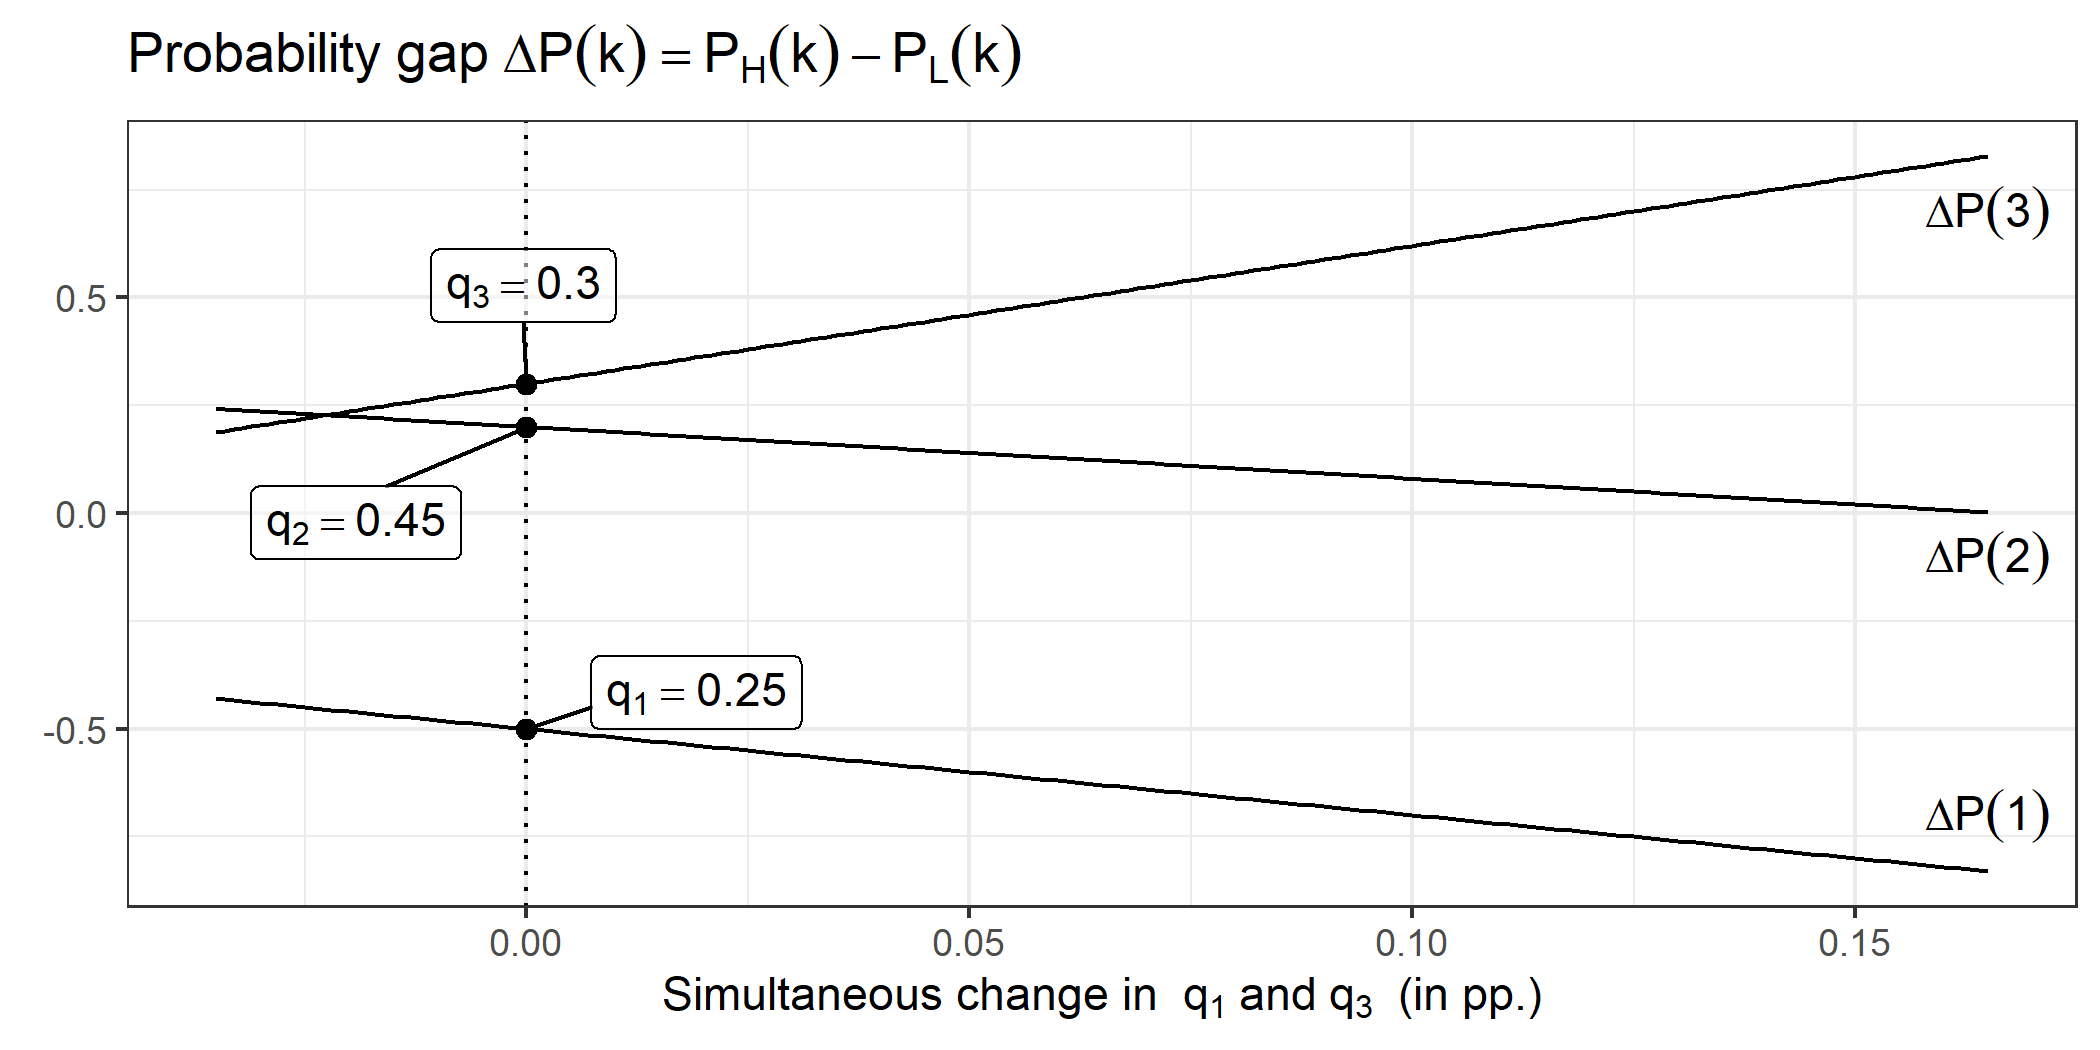
\includegraphics[width=\linewidth]{chap2/graphic/theory-proba-gap.png}
	\vspace{-3em}
	\justify\singlespacing\footnotesize{\textit{Notes:} This figure presents the probability gap in second-period occupations between children from $H$ and $L$ parental income, i.e. $\Delta P(k)$, according to changes in the share of low- and high-paying jobs, i.e. $q_1$ and $q_3$.
	Changes in $q_1$ and $q_3$ are of equal magnitude and at the expense of $q_2$ since $q_1+q_2+q_3=1$.
	Parameters of the model are set such that $z_L = 0.5$, $z_H = 0.5$, and $\pi = 0.25$. The dotted line represents the baseline occupational distribution where $q_1=0.3$, $q_2=0.45$, and $q_3=0.25$.}
\end{figure}
The initial distribution of occupations is assumed to be such that 25\% of workers are in low-paying, 45\% in middling, and 30\% in high-paying occupations. These are figures close to those found in the data, as we will see below. To capture polarization we increase simultaneously $q_{1}$ and $q_{3}$ by the same amount, reducing $q_2$ until only 15\% of workers are in middling occupations (and 40\% and 45\% in $q_1$ and $ q_3$ respectively). The horizontal axis depicts the change in $q_{1}$ and $q_{3}$ in percentage points.

The figure indicates that as polarization increases the advantage in accessing high-paying occupation that those from high-income background have relative to those from low-income households rises. The opposite occurs with low-paying occupations, where the relative likelihood of being in such jobs (which is negative, as only $L$-workers are employed in occupation 1) grows in absolute value with polarization. $H$-workers also have an advantage in being in occupation 2 for low level of polarization, but this advantage falls as $q_1$ and $q_3$ increase, and for high levels of polarization there are more $L$-workers than $H$-workers in middling jobs. The reason for this is that as $q_1$ increases, fewer high-ability $L$-workers manage to move to high-paying occupations, raising their likelihood to be in middling occupations and increasing the number of high-paying jobs available for low-ability $H$-workers. \footnote{In the Appendix we examine separately the effect of changes in $q_1$ and $q_3$ and show that an increase in either of them tends to raise the probability gap between the two types of workers.}

Our results imply a negative relationship between the extent of polarization and the degree of occupation mobility. Greater employment polarization---as measured by an increase in $q_{1}$ and $q_{3}$---reduces mobility by making the distribution of occupations of mature workers more dependent on parental background. This relationship could exist both over time or across locations. If two cohorts of workers face different degrees of polarization when they enter the labour market, we expect to find a lower degree of mobility for the one that experienced a lower share of middling jobs. Similarly, when comparing workers in two geographical areas, we expect to find lower mobility for those based in the location where polarization is greatest.
    
    \section{Data and employment polarization} \label{chap2-data}
    \subsection{Sample and variables}

We use two mature British cohort studies that have been widely used by economists and sociologists to examine the extent of mobility in the UK. The National Child Development Study (NCDS58) is a cohort of individuals born during a given week in March 1958. The British Cohort Study (BCS70) is composed of individuals born during a given week in April 1970. Cohort members were born in England, Scotland, Wales and Northern Ireland and participated in several interviews at different points in time over their life. 
\begin{figure}[!tb]
    \centering
    \caption{Dates of interviews}
    \label{chap2-fig:interviews}
    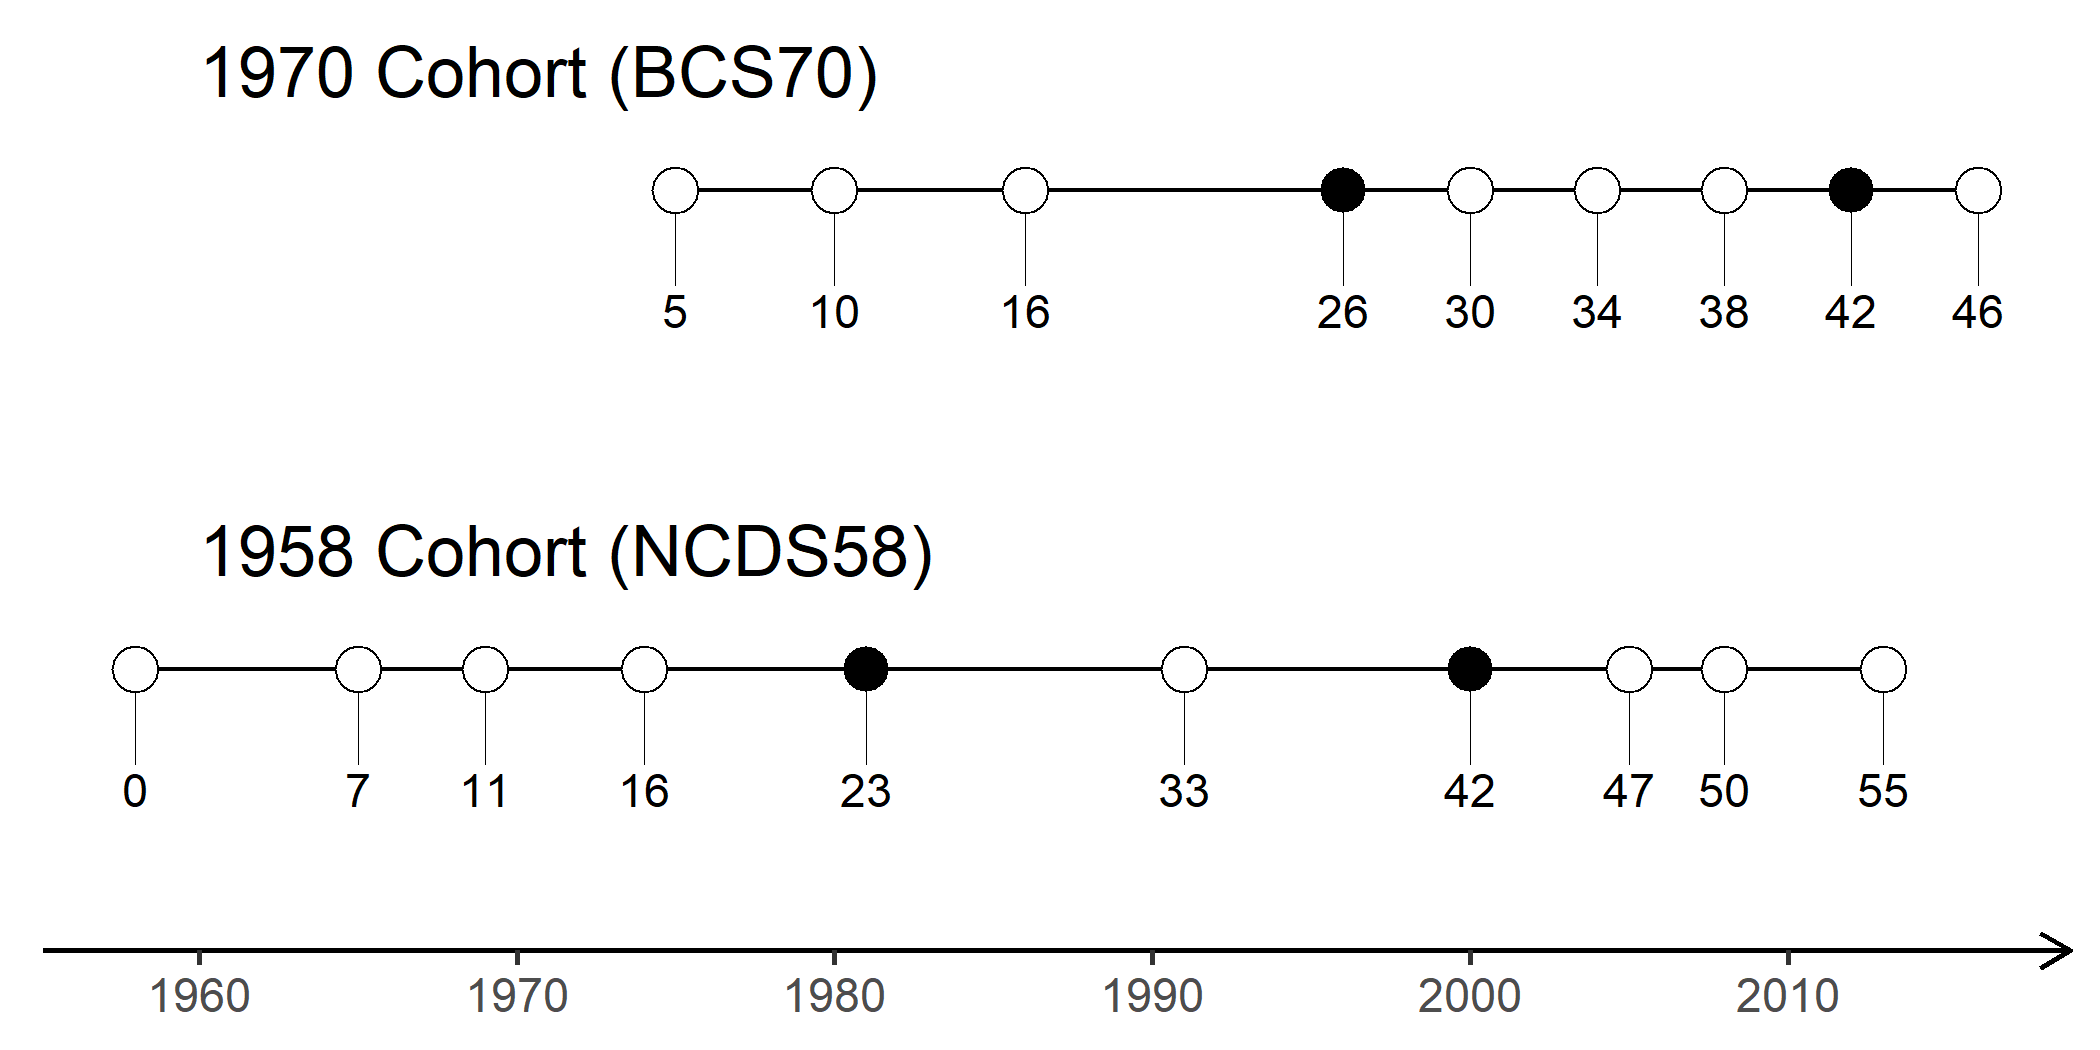
\includegraphics[width=\linewidth]{chap2/graphic/itw-date-spreadpol.png}
	\vspace{-3em}
	\justify\singlespacing\footnotesize{\textit{Notes:} This figure presents the dates at which individuals in the BCS70 and NCDS58 cohorts may have been interviewed and the corresponding years. Black circles represent the first and second periods we consider in the analysis for both cohorts.}
\end{figure}
Figure \ref{chap2-fig:interviews} presents all the interviews at which cohort members were interviewed and the corresponding year.

\textbf{Periods.} We define the first period as the year of interview closest to that in which the individual was 25 years-old, the age usually considered as that of entry into the labour market. Those in the NCDS58 cohort are observed at age 23 and those in the BCS70 cohort at age 26. Both cohorts are interviewed at age 42, which we define as the second period.

\textbf{Income and wages.} We have information on parental income, which is provided when the child was 16 years-old for both cohorts. For the BCS70 cohort, it is also available when the child was 10. Thus, when both are available, we take the average of the two observations; otherwise we use the single one we observe.\footnote{\cite{Blanden2013Intergenerational} show that the observed increase in the role of parental income to determine child's income is not driven by the poor measurement of permanent income in the 1958 cohort.} In order to adjust both for inflation, aggregate income growth and changes in the dispersion of income, parental income is standardized, so that for both cohorts it has mean zero and a variance of 1 (see Table \ref{chap2-tab:stat-indiv} for the summary statistics).

For children, we observe wages, which are reported at each wave. We adjust for inflation using the consumer price index provided by the \href{https://www.ons.gov.uk/economy/inflationandpriceindices}{UK Office for National Statistics}. The resulting monetary variables are all expressed in 1970 British pounds. 

% International Standard Classification of Occupations 1988 (ISCO-88)
\textbf{Occupational categories.} Both cohorts studies provide the full activity histories to the nearest month from which we can derive the ISCO-88 occupations.\footnote{Cohort data provide 3-digit occupations in the \href{https://www.hesa.ac.uk/support/documentation/occupational/soc90}{Standard Occupational Classification 1990 (SOC90)} and the \href{https://www.hesa.ac.uk/support/documentation/occupational/soc2000}{Standard Occupational Classification 2000 (SOC2000)}. We can derive ISCO-88 occupations by using the files from \href{http://www.camsis.stir.ac.uk/occunits/distribution.html}{CAMSIS project} which cover both SOC occupational unit codes and translations into ISCO-88.}
We aggregate ISCO-88 occupations into three categories: high-paying, middling and low-paying occupations. This classification follows the job-polarization literature and is consistent with that used in \cite{Goos2014Explaining} and \cite{Mahutga2018Job}.\footnote{A large body of literature on social mobility relies on the National Statistics Socio-Economic Classification (NS-SEC), starting with \cite{Erikson1992Constant} and \cite{Rose1998ESRC}. However, such classification uses a definition of routine occupations that does not match that used in the job-polarization literature. For instance, the NS-SEC considers that an employee in the 3-digit occupation \textit{Bar staff (622)} has a routine occupation. However, it cannot be considered as a routine job following the definition of \cite{Autor2003Skill} who define this type of job as a non-routine interactive job. We hence chose not to rely on the NS-SEC for our analysis.} Table \ref{chap2-tab:data-isco88} in the appendix presents the classification.  For completeness, we also include a fourth category---individuals who are out-of-work. This category groups those out of the labour force, those who are unemployed, and those in full-time study. Table \ref{chap2-tab:stat-cohper} displays the shares of the various activity status and occupational categories in the cohort data.

As has been shown in previous work, occupational categories are closely related to remuneration levels, and we document this for our cohort data in the appendix. Table \ref{chap2-tab:stat-pay} reports the average weekly pay by occupation, and displays the expected correlation between occupations and pay. 

\textbf{Location.} Since individuals give their address at each interview, we also have their location history. We focus on the region of residence at the age of 16 because it is the age at which the parental income variable is defined. The classification is prior to 1994 and thus uses the Government Offices for the Regions (GORs). We therefore rely on the Standard Statistical Regions (SSR).\footnote{For England, this is the highest sub-national division, while the other countries in Britain consists of a single region. The regions are (in alphabetical order): East Anglia, East Midlands, North, North West, Scotland, South East, South West, Wales, West Midlands, and Yorkshire and Humberside.} Table \ref{chap2-tab:stat-location} reports the share of cohort members in each region for both periods.

Once we restrict the data to those individuals for whom we have the key characteristics, i.e. parental income and occupations, our sample consists of 6,780 individuals in the NCDS58 and 7,983 in the BCS70, as reported in Table \ref{chap2-tab:stat-indiv}.

\textbf{The Labour Force Survey.} As a complementary dataset we use the Labor Force Survey (LFS). The LFS provides data on both labour market status and region of residence. It has the advantage of containing a much larger number of observations (see Appendix \ref{chap2-app-data-LFS} for the details), and allows us to compare the changes in the occupational structure in the cohort data with those from a larger sample, as well as to compute measures of polarization at the regional level.


\subsection{The structure of employment}

% Contribution - alternative view of polarization to the usual snapshot
Before proceeding to our empirical analysis, we consider the extent to which the two cohorts experienced different degrees of polarization. We start by looking at the change in the distribution of occupations at ages 23/26 and 42 for both cohorts, reported in Figure \ref{chap2-fig:stat-occ}.\footnote{We report the proportion of individuals in each occupation for the two cohorts in Tables \ref{chap2-tab:proba-group4-abs} and \ref{chap2-tab:proba-group5-abs} in the appendix.} In the first period there is an increase across cohorts in the probability of working in a high- and low-paying occupation and a decline in that of working in a middling-paying occupation. When we consider the occupations at age 42, the changes are of smaller magnitude, and the main difference across the two cohorts is a reduction in the share of middling jobs that has been offset by high-paying ones. These changes are consistent with the literature on polarization in the UK that shows a considerable decline in middling jobs, and an increase in the other two categories, which is particularly large for high-paying jobs (see Figure \ref{chap2-fig:lfs-national} in the appendix). The differences between the first and second period distributions are interesting for our purposes, as they raise the question of whether polarization in the first period matters even when the changes in the distribution of employment are small for mature individuals. 
\begin{figure}[!tb]
    \centering
    \caption{Occupation distribution across cohorts}
    \label{chap2-fig:stat-occ}
    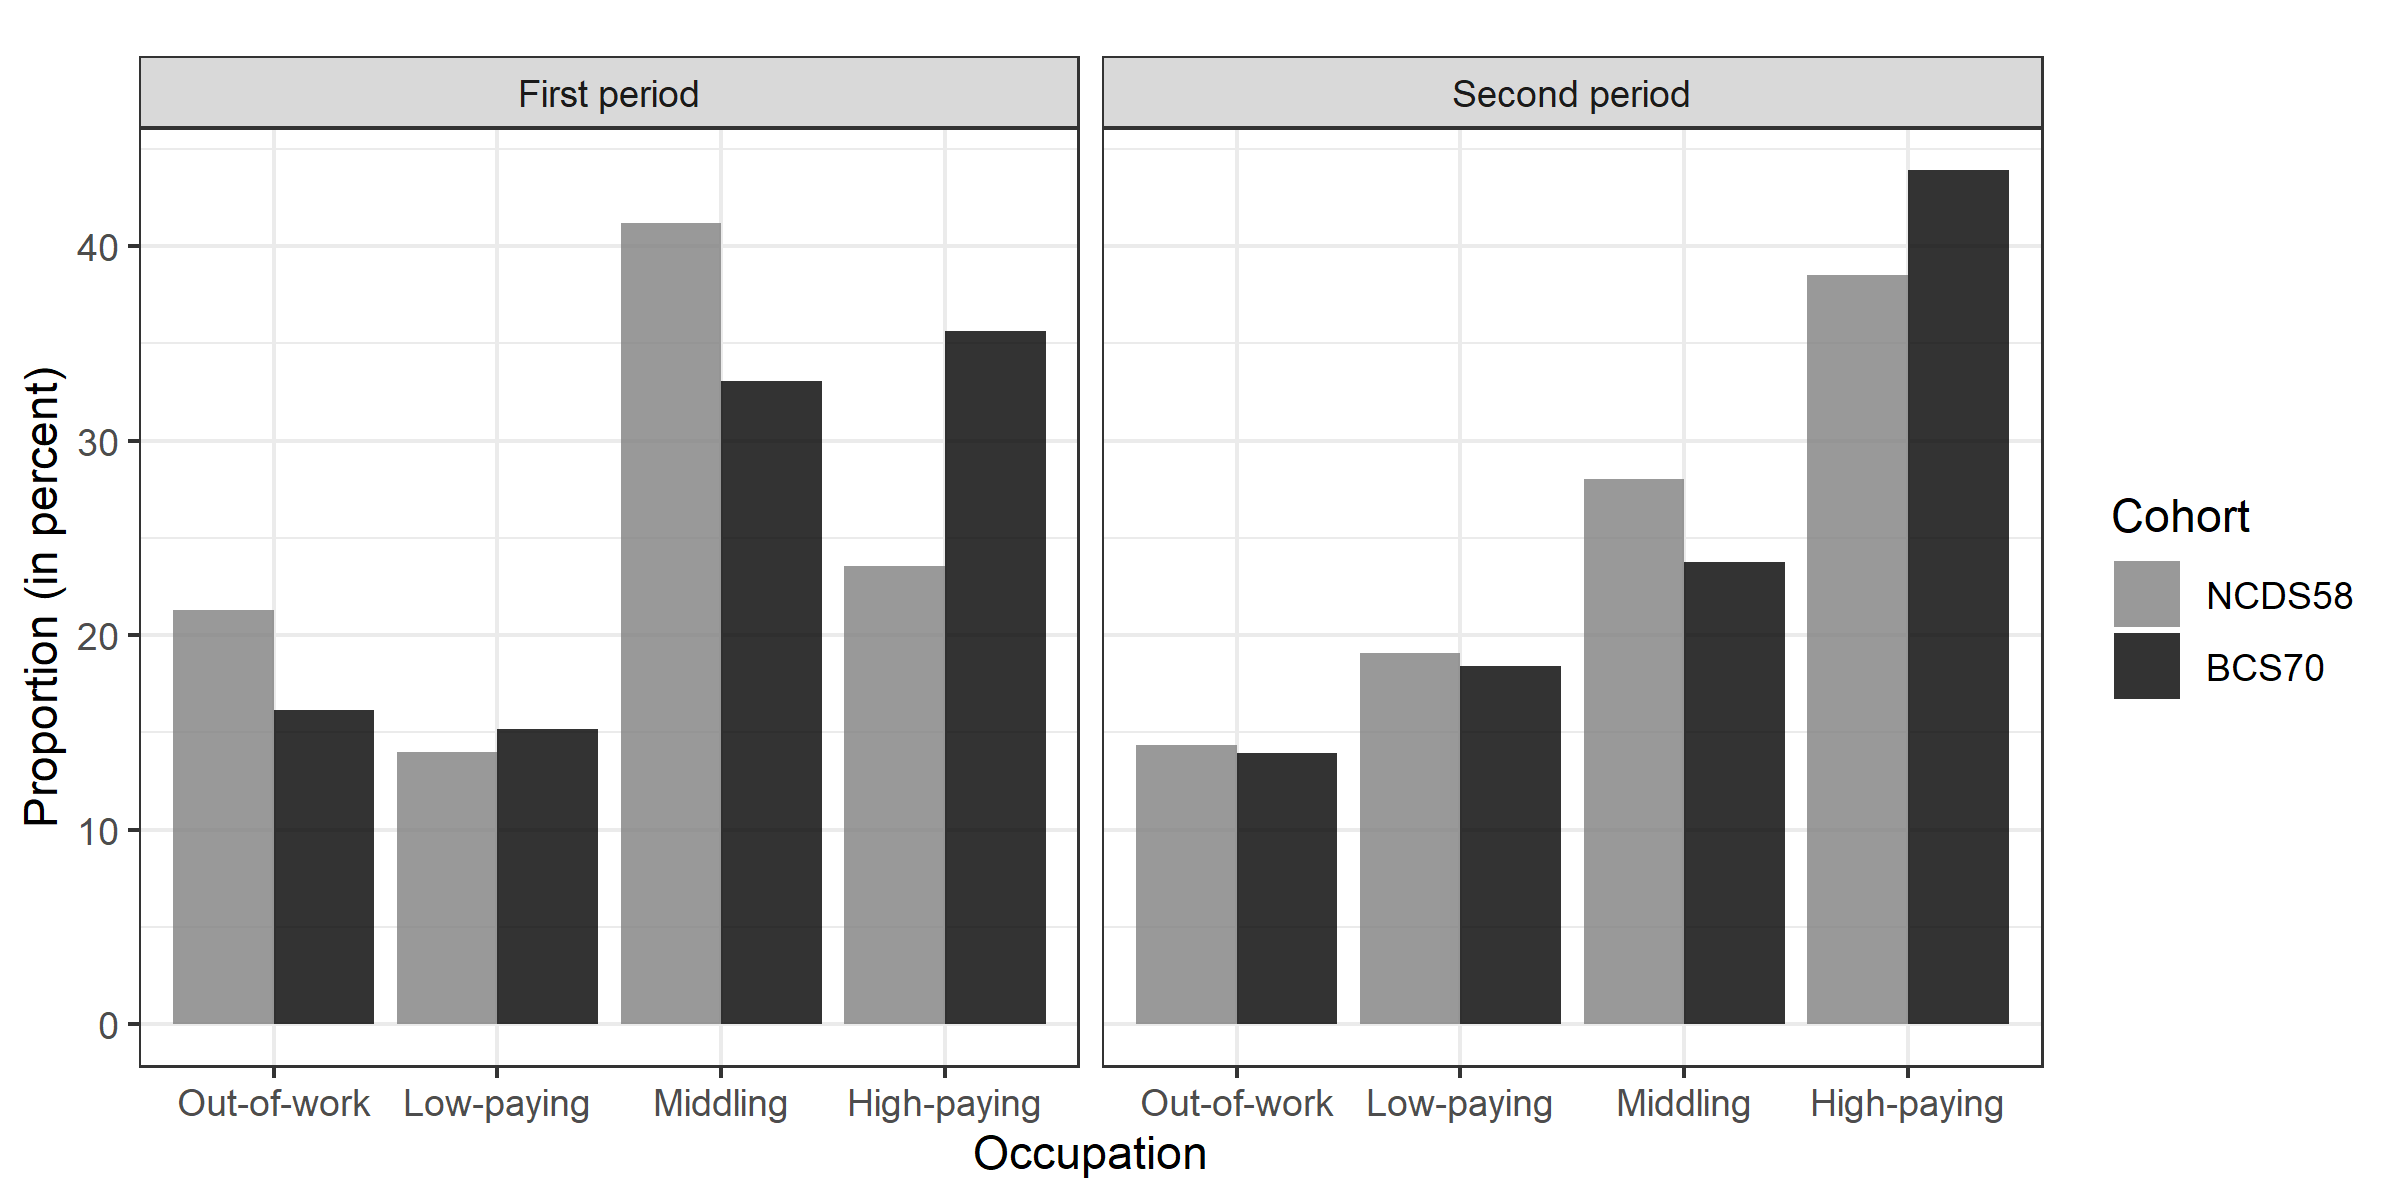
\includegraphics[width=\linewidth]{chap2/graphic/stat-occ.png}
	\vspace{-3em}
	\justify\singlespacing\footnotesize{\textit{Notes:} This figure reports the proportion of individuals, expressed in percent, in each type of occupation (out-of-work, low-paying, middling, high-paying) for the NCDS58 and BCS70 cohorts according to the period.}
\end{figure}
To better understand these dynamics, Figure \ref{chap2-fig:polarize-isco88-both} in the Appendix performs a similar exercise using the ISCO-88 categories, and shows a clear pattern of polarization, which has been particularly large for young individual.

As an alternative way of thinking about polarization we examine how occupations with either different average pay or  ``routine task intensity'' (RTI) have changed across the two cohorts, reported in Figure \ref{chap2-fig:polarize-both-p1}. The left panel depicts the change in the share of individuals in each occupation when young and plots it against the average pay in that occupation (for young individuals of the 1970 cohort). The occupations are depicted by both their code and a geometric symbol, were the latter indicate whether they are in our category of low-paying (circle), middling (triangle) or high-paying (square) occupations. As can be seen from the fitted curve, there is a U-shaped relationship between weekly pay and the change in the share of the occupation, with both those with low and those with high remuneration gaining employment shares at the expense of those in the middle.
\begin{figure}[!tb]
    \centering
    \caption{Change in the probability of being in each ISCO-88 occupation in the first period}
    \label{chap2-fig:polarize-both-p1}
    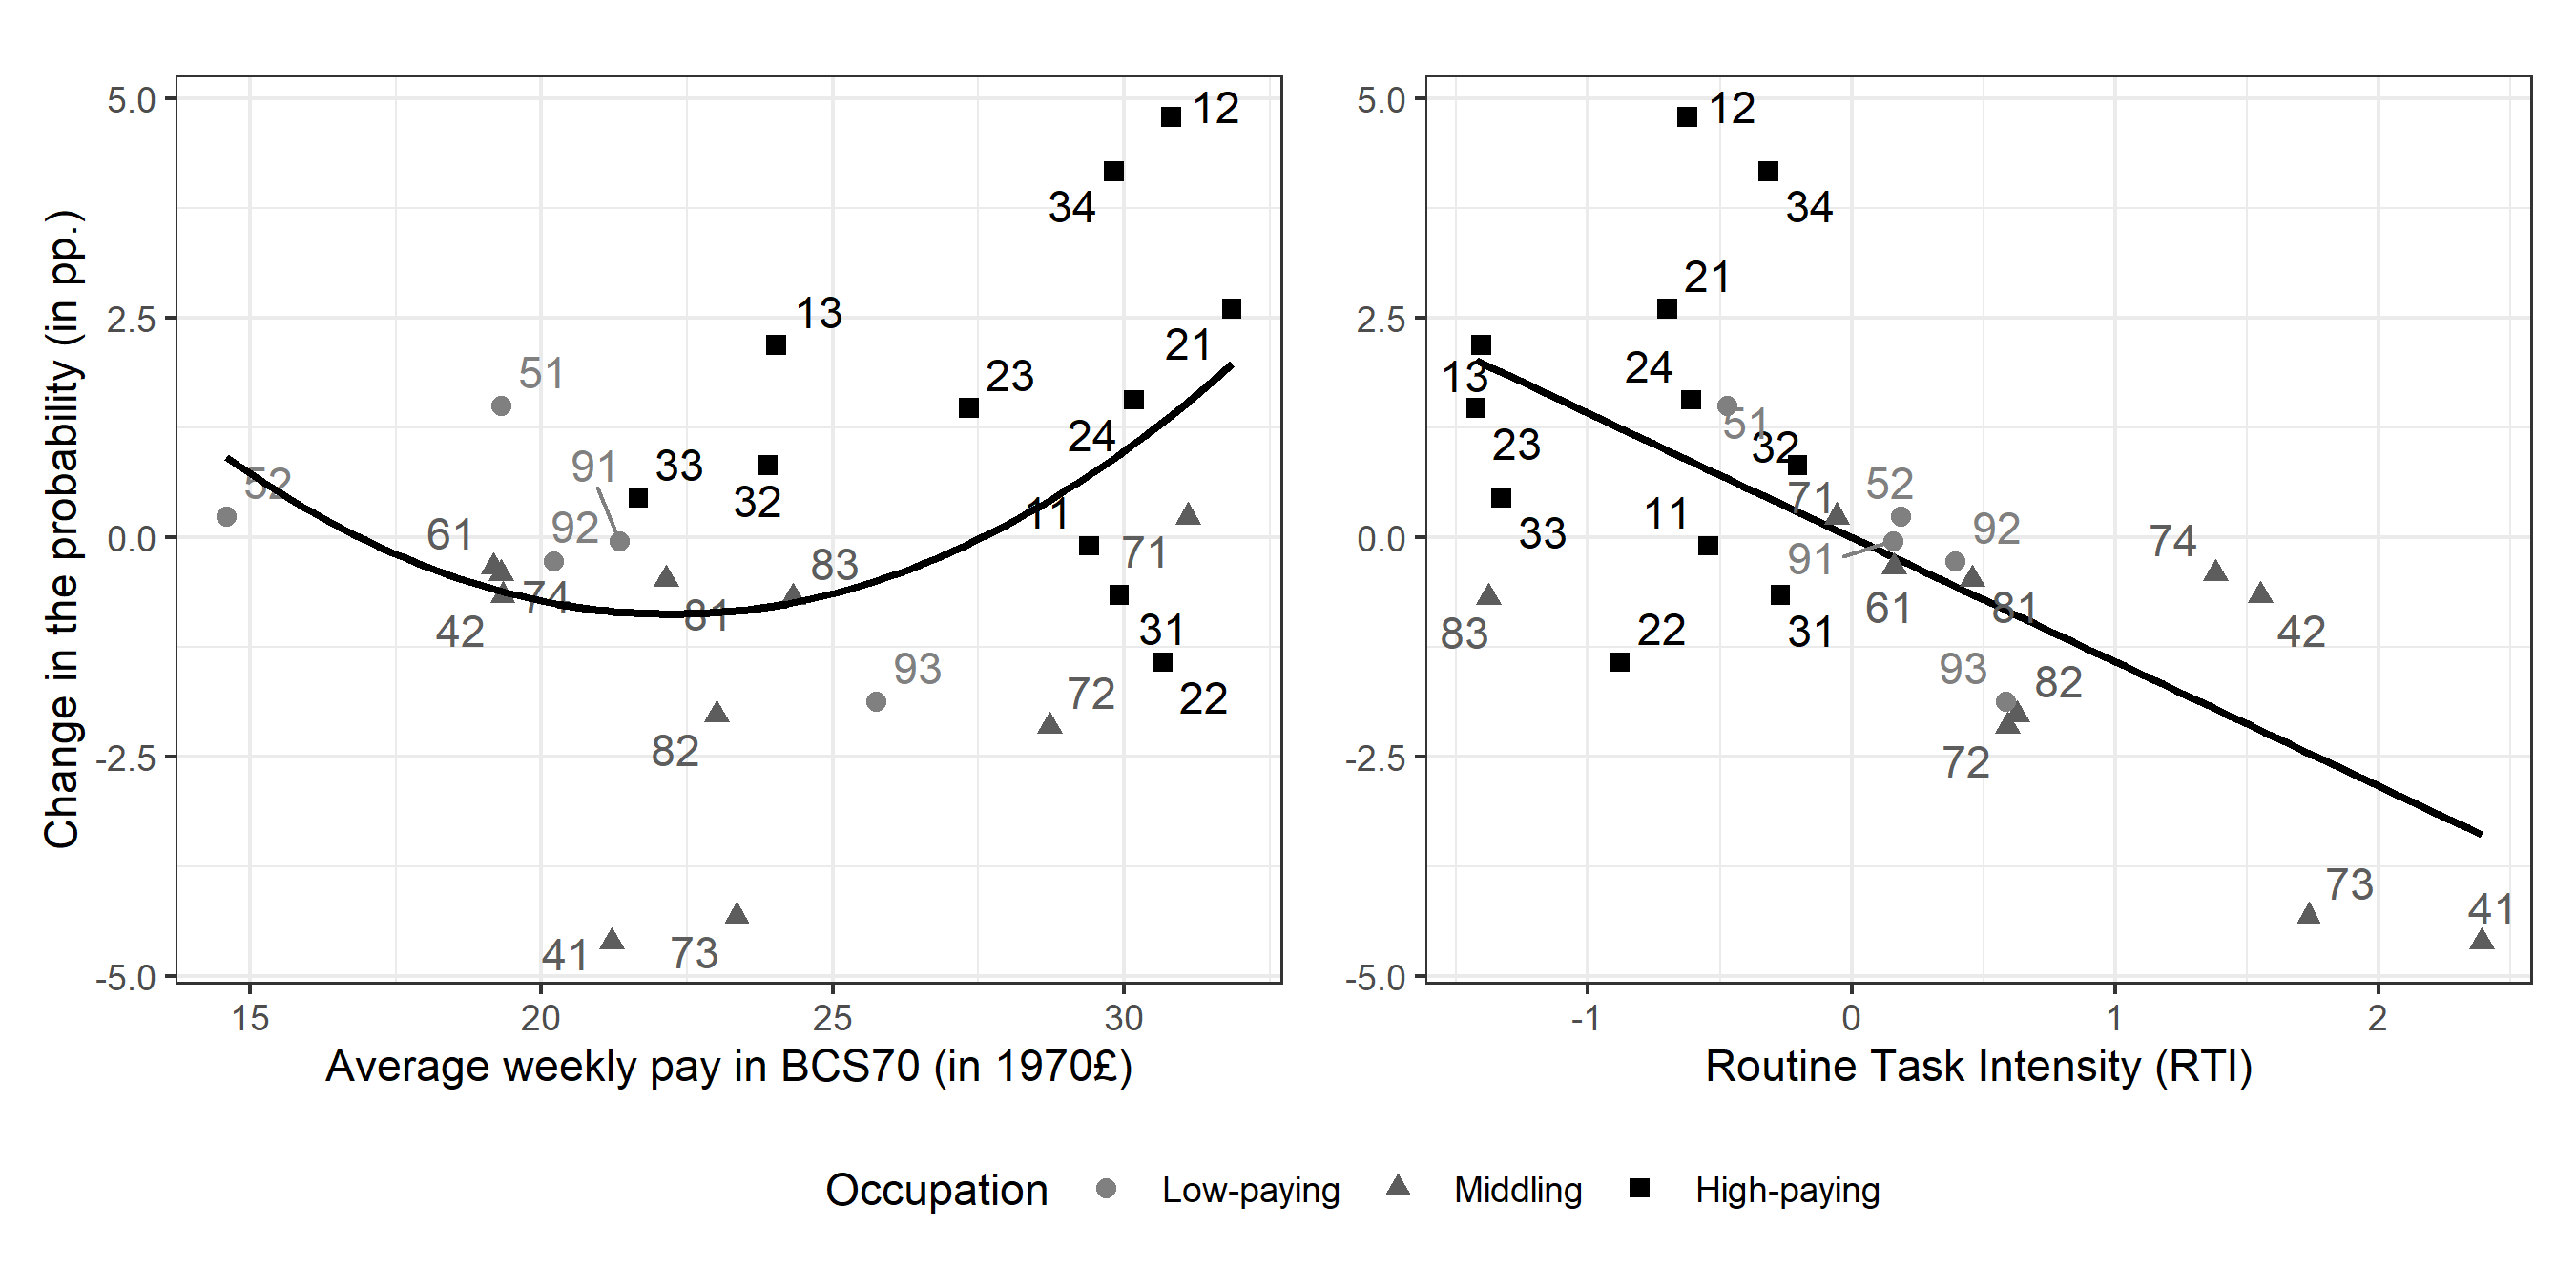
\includegraphics[width=\linewidth]{chap2/graphic/polarize-both-p1.png}
	\vspace{-3em}
	\justify\singlespacing\footnotesize{\textit{Notes:} The left-hand side panel of the figure presents the U-shaped relationship between the difference, expressed in percentage points, between the BCS70 and NCDS58 cohorts in terms of probability of being in each ISCO-88 occupation in the first period and the average weekly pay, expressed in 1970\pounds, in this occupation for the BCS70 cohort. The right-hand side panel shows the negative relationship between the difference, expressed in percentage points, between the BCS70 and NCDS58 cohorts in terms of probability of being in each ISCO-88 occupation in first period and the Routine Task Intensity (RTI) index from \cite{Mahutga2018Job}.}
\end{figure}
The right panel plots the change in the share of each occupation for young individuals against the RTI index provided by \cite{Mahutga2018Job}. The downward slopping line in Figure \ref{chap2-fig:polarize-both-p1} corresponds to the fitted curve implied by the data, and indicates that the change is negatively correlated with the degree of routinization. 

The various pieces of evidence in this section thus indicate that the strong polarization identified in cross-sectional data by previous work is also present when we focus on two specific cohorts. Routine intensity seems to be highly correlated with changes in the share of occupations, with low RTI ones having gained share and those with high RTI having lost it. Moreover, polarization appears whether we use the RTI index to categorize occupations or when we look at average weekly pay.

\subsection{Occupational dynamics} \label{chap2-dynamics}

While the literature on inter-generational mobility has traditionally focused on the outcomes of children when they are mature, we are interested in the occupational dynamics through which individuals reach a particular outcome. To illustrate why this is important, Table \ref{chap2-tab:proba-group4-cdt} reports the conditional probabilities of switching occupations between age 23/26 and age 42.\footnote{To understand why the probability of moving from out-of-work into a high-paying occupation is so high, recall that the former category includes those in education. Conditional probabilities in which we consider those in education as separate category, hence not included in out-of-work, are reported in the appendix, and display the expected (large) difference between those in education and the rest of those out-of-work; see Table \ref{chap2-tab:proba-group5-cdt-short}.}

\begin{table}[!tb]
    \centering
    \caption{Conditional probabilities of changing occupations}
    \label{chap2-tab:proba-group4-cdt}
    \begin{threeparttable}
        \small
        
\begin{tabular}{lrrrrrrrr}
\toprule
\multicolumn{1}{c}{} & \multicolumn{4}{c}{BCS70} & \multicolumn{4}{c}{NCDS58} \\
\cmidrule(l{3pt}r{3pt}){2-5} \cmidrule(l{3pt}r{3pt}){6-9}
Occupation & Out & Low & Mid & High & Out & Low & Mid & High\\
\midrule
Out-of-work & 33.8 & 25.3 & 14.5 & 26.4 & 27.4 & 24.7 & 20.7 & 27.3\\
Low-paying & 13.6 & 45.1 & 17.5 & 23.8 & 16.3 & 40.0 & 20.3 & 23.4\\
Middling & 10.5 & 13.8 & 44.9 & 30.8 & 10.4 & 15.4 & 43.4 & 30.8\\
High-paying & 8.3 & 8.2 & 11.0 & 72.6 & 8.5 & 8.1 & 12.3 & 71.2\\
\bottomrule
\end{tabular}

        \begin{tablenotes}[flushleft]
            \footnotesize{\item \textit{Notes}: This table shows the probability, expressed in percent, of being in each second-period occupation (columns) conditional on the first-period occupation (rows) for individuals in the NCDS58 and BCS70 cohorts.}
        \end{tablenotes}
    \end{threeparttable}
\end{table}

The table shows that there is a considerable degree of mobility across occupations over the individual's lifetime, i.e. of intra-generational mobility. Individuals who start their careers in low-paying and middling occupations have probabilities of staying there of around 40\% and a substantial likelihood of moving upwards. Notably, 30.8\% of those initially in middling occupations have a job in high-paying occupations by age 42 for both cohorts. In contrast, persistence is high for those who start in high-paying occupations, over 70\%. The transition probabilities are remarkably similar across cohorts, in particular those of moving into a high-paying occupation. The most significant differences come from the outcomes of those who start either out of work or in low-paying occupations. In both cases, those in the younger cohort face a lower probability of being in a middling occupation when mature (lower by 5.8 and 2.5 pp., respectively) which translates into higher odds of remaining in the occupation of origin. 

These figures indicate that the occupational outcomes of mature individuals depend both on their initial occupations and on the transitions across occupations, and raise the question of whether a reduction in the share of middling jobs can be a break to mobility. If mobility occurs partly through individuals progressing up the income ladder during their careers, the disappearance of middling jobs can have important consequences. On the one hand, a large proportion of those who are in high-paying occupations at age 42 start their careers in middling occupations. If fewer individuals are in such occupations when young, as indicated by Figure \ref{chap2-fig:stat-occ}, then there will be fewer individuals that can move into high-paying jobs. On the other, those who start in low-paying occupations have access to fewer middling jobs and hence are more likely to stay in their initial occupations. The importance of such changes for mobility will depend on the extent to which parental background matters for entry into each occupation and for the subsequent dynamics.

    
    \section{Empirical specification} \label{chap2-specification}
    Our analysis proceeds in two steps. The first consists in examining how an individual's occupation is affected by parental background. As we will detail in the next subsection, we suppose that this impact can potentially occur both through the effect on the child's initial occupation and on her occupation as a mature worker. In a second step, we consider regional patterns of mobility and assess to what extent regional differences in polarization are correlated to observed mobility patterns at the regional level.

\subsection{The determinants of individual mobility} \label{chap2-specification1}

In order to understand the effect of parental income on occupational dynamics we start by estimating its impact on the child's probability to start her career in each occupation $j\in J = \{O, L , M, H\}$, where the possible occupations are out-of-work ($O$), low-paying ($L$), middling ($M$) and high-paying ($H$). We define the out-of-work occupation as the baseline occupation category. Let $p_j$ be the probability to start in occupation $j = \{L , M, H\}$ which is given by the following multinomial logistic model:
\begin{equation}\label{chap2-eq:emp-multi1}
    \log\left(\frac{p_j}{p_O}\right) = \alpha_{1j} + \beta_{1j} Y^p + \gamma_{1j} X,
\end{equation}
where $Y^p$ is parental income, and $X$ are individual characteristics (in our baseline specifications simply gender). Parental income is log-standardized. All terms will be interacted with a dummy that equals one for those in the 1970 cohort (BCS70) and zero otherwise. Cross-term coefficients hence represent the change across cohorts in the effect of the variable on the child's initial occupation. In the appendix, we also report the estimation of the four binomial logistic models that characterize the multinomial one.

We next consider the determinants of the probability of being in occupation $k \in K = \{O, L , M, H\}$ at age 42. The simplest specification is to consider a specification of the form
\begin{equation}\label{chap2-eq:emp-multi2}
    \log\left(\frac{p_k}{p_O}\right) = \alpha_{2k} + \beta_{2k} Y^p + \gamma_{2k} X,
\end{equation}
which captures how parental income determines the occupational outcome of the mature child. This expression is consistent with the approach usually found in the literature on inter-generational mobility in which only the labour market outcome of the mature worker is considered. In contrast, intra-generational analyses have focused on how incomes evolve over the individual's working life. We hence consider the following specification: 
\begin{equation}\label{chap2-eq:emp-multi3}
    \log\left(\frac{p_k}{p_O}\right) = \alpha_{3k} + \sum_{j} \eta_{kj} \mathbb{1}_{j} + \beta_{3k} Y^p + \gamma_{3k} X,
\end{equation}
where $\mathbb{1}_{j}$ is a dummy variable that equals one when the individual was in occupation $j\in J$ when young. As before, we estimate second-period equations with a multinomial model and separately for the four occupations using binomial logistic regressions, which we report in the appendix.

The expression in equation (\ref{chap2-eq:emp-multi3}) shares with the literature on intra-generational mobility the idea that individual's may change position in the income ladder and that it is important to understand how those dynamics operate. It differs from existing approaches in two respects. First, we focus on occupational mobility over the lifetime, rather than income mobility; second, we control for parental income as a potential factor that can influence the extent to which the child changes occupations over time. Equation (\ref{chap2-eq:emp-multi3}) then adds to the literature on intra-generational mobility by allowing parental income to have an impact on lifetime occupational changes, and to that on inter-generational mobility by allowing the effect of parental income on the occupation of mature workers to occur both through their initial occupation and through the likelihood of transition to other jobs.  

Our empirical strategy makes two important choices. The first is not to consider education decisions and to focus exclusively on the direct impact of parental income. The alternative approach would be to consider a three-step setup in which parental income determines education, which then determines first-period occupation, which in turn determines the second-period job.\footnote{A large literature has considered the role of education for social mobility, and in particular examined to what extent the influence of parental background takes place through educational achievement. Examples of this literature are \cite{Blanden2004Family}, \cite{Blanden2014Education}, \cite{Blanden2016Educational}, \cite{Gregg2010Family} and \cite{Major2018Social}.} The advantage of the latter approach is that it would allow us to infer how much of the parental-income advantage operates through education and how much is a direct effect; the drawback is that educational attainment is correlated with unobservable characteristics, notably ability but also the type of school attended, hence the effect that we may be attributing to years of education could be capturing other aspects, whether innate or related to parental background.\footnote{See \cite{harmon2003returns} for a discussion of the difficulty of differentiating between the returns to education and those to (innate or socially-acquired) ability.} We hence focus exclusively on the two occupational outcomes, although we perform the three-step analysis in Appendix \ref{chap2-app-education}.

Second, we have chosen to use a multinomial logistic model considering the four possible occupational outcomes and where our reference outcome is being out-of-work. It is important to note that the transition from this category into the three employment occupations occurs with roughly equal probabilities. Notably, for the NCDS58 (BSC70) the probability of transiting from out of work to low- and high-paying occupations was, respectively, 24.7 pp. (25.3 pp.) and 27.3 pp. (26.4 pp.), i.e. of very similar magnitude. The likelihood to move into middling occupations was somewhat lower (20.7 and 14.5 pp.) but of comparable magnitude; see Table \ref{chap2-tab:proba-group4-cdt} above.

\subsection{Mobility and regional polarization}

The second step of our analysis consists in exploring the relationship between the observed changes in the role of parental income and polarization. We do so by examining whether changes in regional mobility are correlated to changes in the extent of polarization at the regional level. To do so we run a multinomial regression at the regional level for the determinants of the probability of being in occupation $k \in K = \{O, L , M, H\}$ at age 42. We do not compute first-period mobility and conditional second-period mobility because of sample sizes, as in many regions we have only a small number of individuals moving across certain occupations between first and second period. The equation we estimate is hence
\begin{equation}\label{chap2-eq:regocc-multi2}
    \log\left(\frac{p^r_k}{p^r_O}\right) = \alpha^r_{k} + \beta^r_{k} Y^p + \gamma^r_{k} X,
\end{equation}
where \emph{r} denotes the region. We hence use individual data to estimate 10 coefficients $\beta^r_{k}$ that capture the impact of parental income on occupational outcomes in each of the regions.

As we will see below, our estimates indicate that the dynamics of the impact of parental income vary across regions, with the change across generations being much larger in some than in others. The last step in our analysis is hence to construct a measure of regional polarization and compute its correlation with our regional estimates. To capture changes in mobility in region $r$, we consider the between-cohort change in the role of parental income for being in occupation $k$, namely, $\Delta\beta_k^r$. We hence compute the correlation between mobility and polarization by running the regression
\begin{equation}\label{chap2-eq:reg-multi2}
    \Delta\beta_k^r = \delta_{k} + \eta_{k} \Delta Pol^r,
\end{equation}
where $Pol^r$ is a measure of polarization at the regional level for a particular cohort and $\Delta Pol^r$ its change across cohorts. The measure of polarization will be constructed using the Labour Force Survey in order to have larger regional samples than those provided by the cohort data \footnote{The measure of polarization used is discussed is detail in section \ref{chap2-regional} below, and Appendix \ref{chap2-app-data-LFS} gives details on the data used.} 








    
    \section{Patterns of mobility} \label{chap2-mobility}
    \subsection{Initial occupations} \label{chap2-initial}

We start by estimating the impact of parental income on the child's first-period occupations, before considering the occupation of mature individuals in the next section. We estimate equation \eqref{chap2-eq:emp-multi1} and report the results in the appendix, those for the binomial logits are reported in Table \ref{chap2-tab:occ-bi1-base} and the multinomial results in Table \ref{chap2-tab:occ-multi1-base}.  Logit coefficients are hard to interpret, hence to visualize the results Figure \ref{chap2-fig:occ-multi1-pinc} displays the probability to be in each occupation when young as a function of parental income.
\begin{figure}[!tb]
    \centering
    \caption{First-period occupation probability according to parental income}
    \label{chap2-fig:occ-multi1-pinc}
    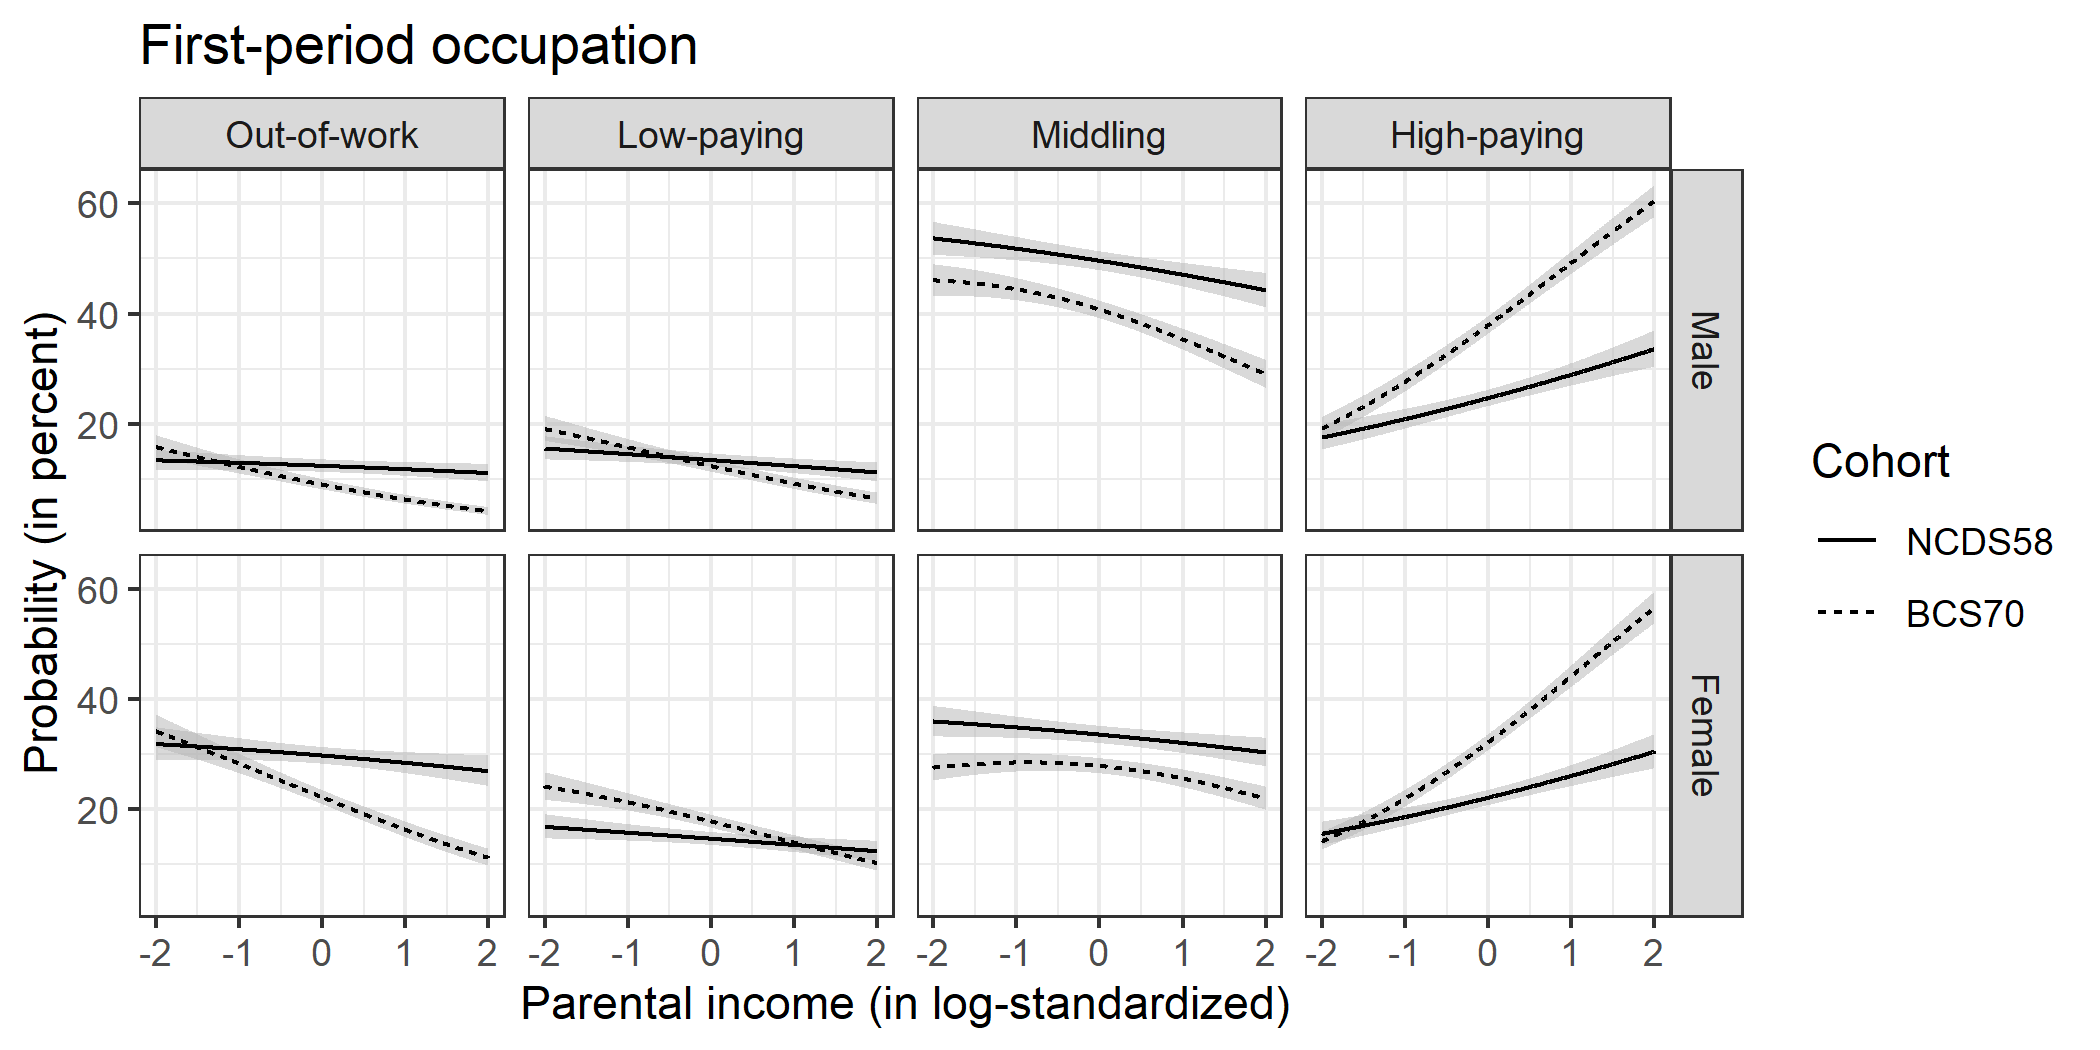
\includegraphics[width=\linewidth]{chap2/graphic/occ-multi1-pinc.png}
    \vspace{-3em}
	\justify\singlespacing\footnotesize{\textit{Notes:} This figure presents the probability, expressed in percent, of being in each type of occupation (out-of-work, low-paying, middling, high-paying) in first period according to parental income, in log-standardized.
	Probabilities are computed for males and females in both cohorts according to the multinomial logistic regression reported in Table \ref{chap2-tab:occ-multi1-base} in the appendix.}
\end{figure}
The probabilities are computed according to the multinomial logistic regression, but the results are qualitatively equivalent when using the binomial estimates. The probabilities are reported separately for the two cohorts and for the two genders; the four columns depict the four possible outcomes, starting with out-of-work occupations on the left.

Consider first the outcomes for the 1958 cohort, depicted by the continuous lines. Parental income is a key determinant of initial occupation, with high income increasing the probability to be in a high-paying occupation and reducing that of being in a middling or low-paying one. There is no effect on the probability of being out-of-work (see also Table \ref{chap2-tab:occ-bi1-base}), a result that is not surprising given the various outcomes included in this category. Note also that the effect of family background is particularly large for high-paying occupations. The levels vary across men and women, with women being more likely than men to be out-of-work and less likely to be in any of the three types of employment.

The impact of parental income on the various probabilities for the 1970 cohort are depicted by the dashed lines. Starting with men, Table \ref{chap2-tab:occ-multi1-base} reports large changes across cohorts in the coefficients on the direct effect of parental income, which are captured in the figures. For example, the coefficient doubles for high-paying occupations, increasing from 0.21 to 0.41, a result that is reflected in the large increase in the slope of the schedule that we observe in the two right panels. There are various possible explanations for this. Obviously, the effect could be operating through education which has become more dependent on parental background (see Appendix \ref{chap2-app-education} for a discussion). Other explanations are that non-cognitive skills have become more important and that they are positively associated with the household’s income, or parental income could be a proxy for the child’s social network, either its size or ‘quality’, which in turn has become more important in determining access to jobs.\footnote{For example, \cite{Blanden2007Accounting}, using the same data as us, show a strengthening of the relationship between parental income and non-cognitive skills between both cohorts. \cite{Major2018Social} emphasize the changing role of education and the increasing importance of the "extra-investments" made by upper-middle class families. For the US, \cite{Chetty2014Land} show that neighborhood characteristics are extensively correlated with mobility.}

As expected, the probability of being in a middling occupation has fallen for all individuals, irrespective of family background. The decline has been greater the higher parental income is. Together with the previous result this indicates that as the share of high-paying jobs increased, those from high-income households are more likely to go into high-paying jobs at the expense of middling ones. The probability of being in a low-paying occupation has pivoted around the mean, with those at the bottom (resp. top) of the parental income distribution being more (resp. less) likely to be in that occupation in the 1970 than in the 1958 cohort. The schedule for being out of work displays a steeper slope, with a decline in the probability of being in this category for all men except those at the very bottom of the parental income distribution.

Consider now the schedules for women. Starting from the right, we can see that women experienced a large decline in the likelihood of being out-of-work, consistent with the increase in female labour force participation observed over the period. Yet, the reduction is strongly correlated to parental income, even more so than for men. The probability of being in a low-paying occupation has increased at virtually all points of the distribution---except at the very top---indicating that much of the increase in female participation occurred through access to low-paying jobs. The probability of being in middling occupations has declined for the younger cohort, as is the case for men. Interestingly, for women the schedule is non-monotonic. At the bottom of the parental income distribution, an increase be income raises the probability of being in middle occupations, with the effect then turning negative. This seems to indicate that in the lower segment of the parental income distribution, an increase in income confers women a occupational advantage, allowing them to access middling rather than low-paying jobs. As is the case for men, the slope of the schedule for high-paying occupations has increased sharply across the two cohorts.

These patterns indicate that parental income conferred a greater advantage for those born in 1970 as compared to those born in 1958. Much of the change was driven by reduced entry into middling occupations, which was offset by a greater likelihood to in in a high-paying (resp. low-paying) occupation for those coming from households at the top (resp. bottom) of the parental income distribution.

\subsection{Mature occupations} \label{chap2-mature}

We turn now to the probability of being in occupation $k$ at age 42. Recall that we suppose that as well as depending on parental income, the occupation of mature workers depends on their job at the start of their career. We hence consider both an expression that does not include the effect of initial occupations, as given by equation \eqref{chap2-eq:emp-multi2}, and one in which they are included, as in equation \eqref{chap2-eq:emp-multi3}. The former specification is equivalent to those usually found in the literature.

As before, we estimate this equation both separately for the four occupations as well as in a multinomial regression. The full results are reported in Tables \ref{chap2-tab:occ-multi23-base} and \ref{chap2-tab:occ-bi23-base} in the appendix, while Table \ref{chap2-tab:occ-multi2-short} summarizes the multinomial results for the baseline regression, in which we do not consider the effect of initial occupations.
\begin{table}[!tb]
    \centering
    \caption{Second-period occupation probability}
    \label{chap2-tab:occ-multi2-short}
    \begin{threeparttable}
        \setlength{\tabcolsep}{18pt}
        \begin{tabular}{l D{.}{.}{5.3} D{.}{.}{5.5} D{.}{.}{5.5}}
\toprule
 & \multicolumn{3}{c}{Multinom. logit - Dep. var.: Second-period occ.} \\
\cmidrule(lr){2-4}
 & \multicolumn{1}{c}{Low-paying} & \multicolumn{1}{c}{Middling} & \multicolumn{1}{c}{High-paying} \\
\midrule
Par. inc.              & 0.01   & 0.04       & 0.19^{***} \\
                       & (0.04) & (0.04)     & (0.04)     \\
Par. inc. $\times$ BCS & 0.05   & 0.15^{***} & 0.36^{***} \\
                       & (0.06) & (0.05)     & (0.05)     \\
\midrule
Num. obs. & \multicolumn{1}{c}{14763} & \multicolumn{1}{c}{14763} & \multicolumn{1}{c}{14763}\\
\bottomrule
\end{tabular}

        \begin{tablenotes}[flushleft]
            \footnotesize{\item\textit{Notes}: 
            % Stars and SE
            $^{***}p<0.01$; $^{**}p<0.05$; $^{*}p<0.1$. Standard errors between parentheses. 
            % Baseline outcome
            Out-of-work occupation in second period is the base outcome of the multinomial logistic regression.
            % Referent group
            Male in the NCDS58 cohort in out-of-work occupation in first period is the referent group. 
            % Variables details
            Parental income in logarithm and then standardized at the cohort level. 
            % Control variables
            Control variables in all regressions include Intercept, BCS cohort, Female and Female $\times$ BCS; see Table \ref{chap2-tab:occ-multi23-base} in the appendix for these coefficients.}
        \end{tablenotes}
    \end{threeparttable}
\end{table}

As before, the reference category are those out of work. Parental income has a large impact on occupational outcomes at age 42, with the coefficient for high-paying jobs almost doubling across cohorts. This result is in line with the extensive work that has found an increased correlation in parent-child incomes, as discussed in the introduction. While a one-standard-deviation increase in parental income used to raise the odds to be in a high-paying occupation by 21\% for the older cohort, this same increase raises the odds by 73\% for the younger one.\footnote{These coefficients are obtained by taking the exponential of the change in log odds, i.e. $\exp(0.19) = 1.209$ and $\exp(0.19+0.36) = 1.733$.} 

To illustrate the relationship between parental income and occupational dynamics, Figure \ref{chap2-fig:occ-multi2-pinc} reports the probabilities of being in each occupational category at age 42 as a function of parental income, for both genders.
\begin{figure}[!tb]
    \centering
    \caption{Second-period occupation probability according to parental income}
    \label{chap2-fig:occ-multi2-pinc}
    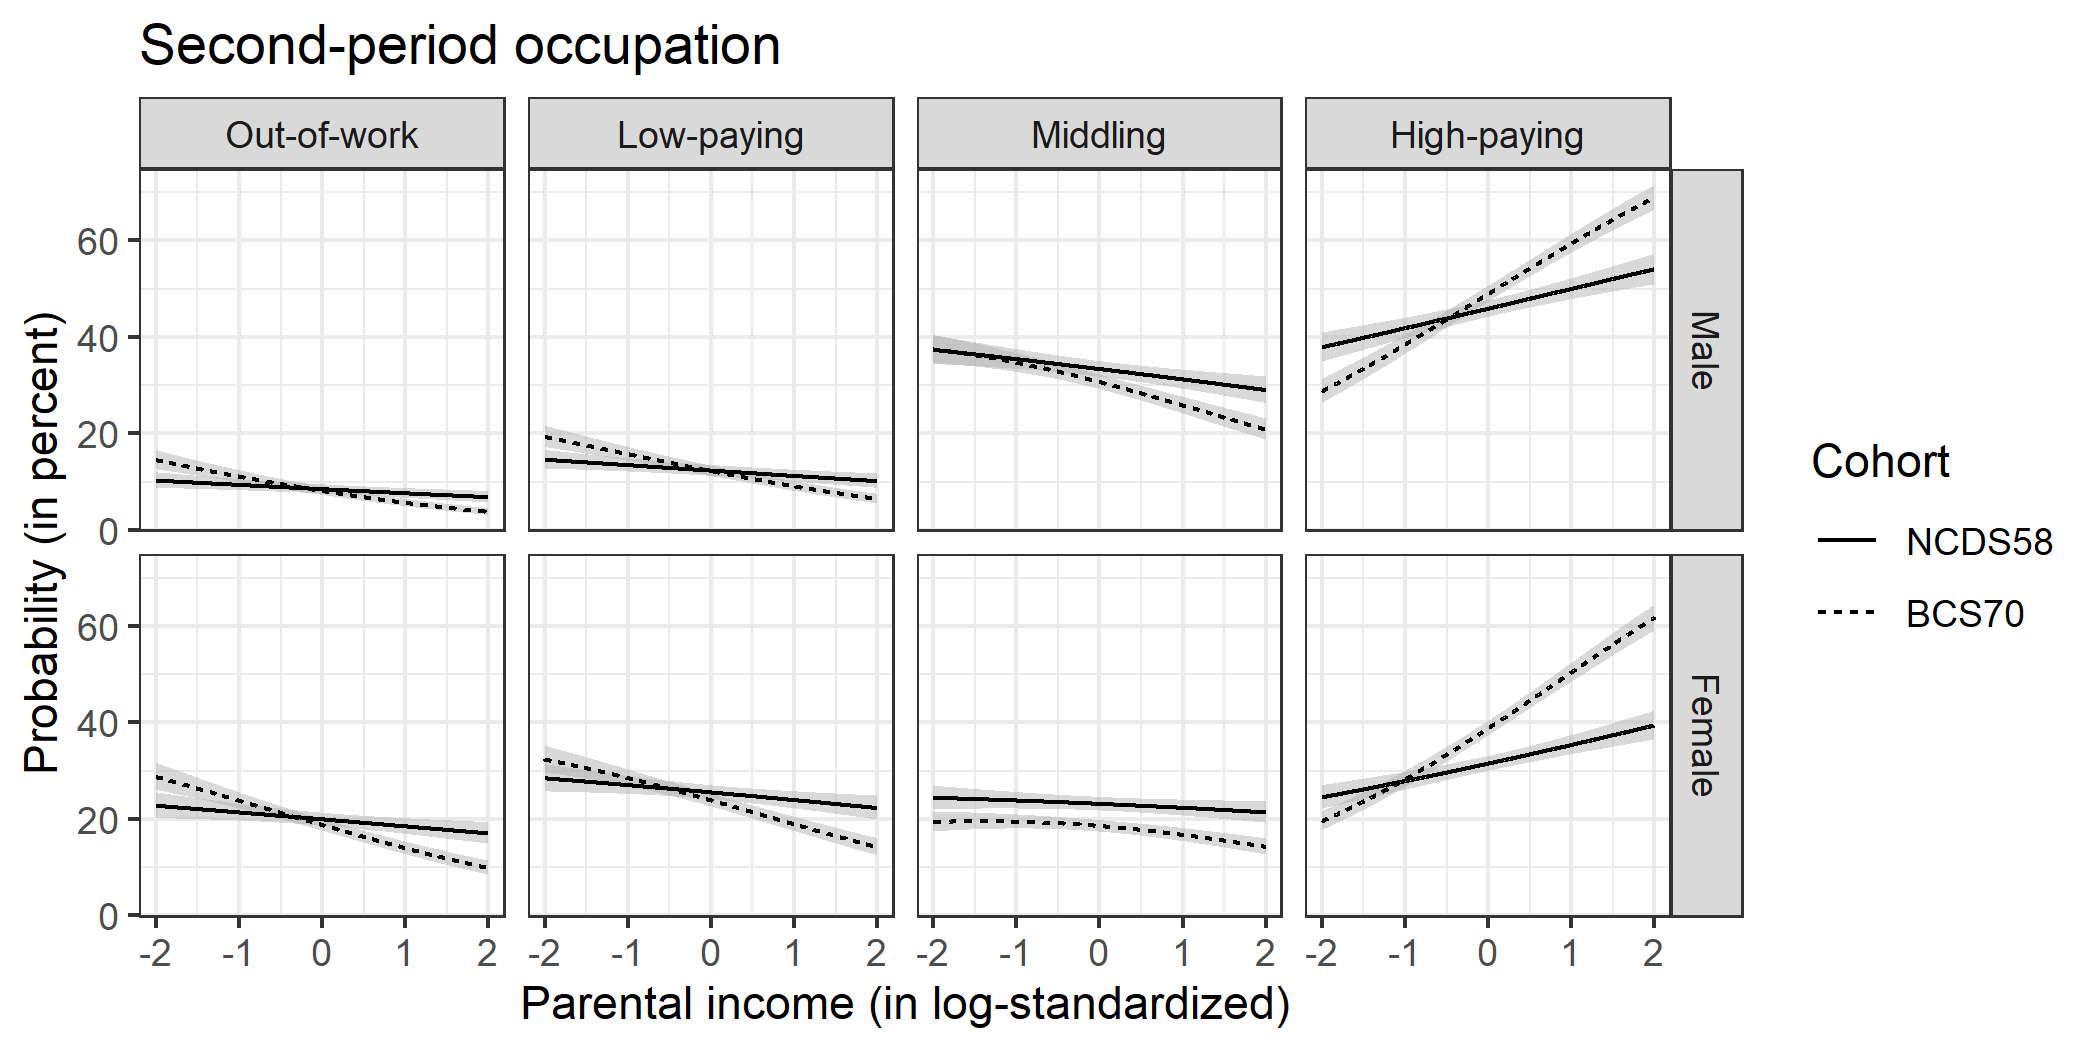
\includegraphics[width=\linewidth]{chap2/graphic/occ-multi2-pinc.png}
    \vspace{-3em}
	\justify\singlespacing\footnotesize{\textit{Notes:} This figure presents the probability, expressed in percent, of being in each type of occupation (out-of-work, low-paying, middling, high-paying) in second period according to parental income, in log-standardized.
	Probabilities are computed for males and females in both cohorts according to the multinomial logistic regression reported in Table \ref{chap2-tab:occ-multi23-base} in the appendix.}
\end{figure}
As for initial occupations, coming from a better-off background increases the probability of being in a high-paying occupation and reduces all others. The main difference with our results for initial occupations is the crossing of several of the probability schedules. Consider the probability of being in a high-paying occupation; we can ask whether individuals from all backgrounds have benefited from the increase in the share of such jobs across the two cohorts. Figure \ref{chap2-fig:occ-multi1-pinc} indicates that, as far as initial occupations are concerned, this is the case, with even those men at the bottom of the parental-income distribution (i.e. 2 standard deviations below the average) exhibiting a larger probability of being in a high-paying job for the younger than for the older cohort. In contrast, we can see in Figure \ref{chap2-fig:occ-multi2-pinc} that by age 42 only those from sufficiently well-off households have reaped the benefits of the expansion in high-paying jobs. Men whose parents had an income 0.5 standard-deviations below the average had the same probability of being in a high-paying occupation in both cohorts; those with lower parental income, experienced a lower probability if born in 1970 than if born in 1958.

Figure \ref{chap2-fig:occ-multi2-pinc} is reminiscent of the analysis in \cite{Major2018Social}, who show, using the same data, that the effect of parental income on the probabilities of being in the various quintiles of the income distribution has increased across the two cohorts (see \cite{Major2018Social}, Figures 0.1 and 0.2). Our results indicate, not surprisingly, that the occupational structure is behind the observed changes in income mobility and closely mimic their findings when we consider the probabilities of being in each of the four occupations for each decile in the parental-income distribution (see Figure \ref{chap2-fig:occ-multi2-quant-male} in Appendix \ref{chap2-app-additional}).


\subsection{From initial to mature occupations} \label{chap2-intra}

The marked change in the overall effect of parental income across the two generations can be due to changes in either how parental income impacts initial occupations or in its effect on mobility during the child's career, i.e. on intra-generational mobility. As we have seen above, the influence of parental background on the former has become stronger; we turn next to whether coming from a better-off background also changes the extent to which, given her initial occupation, an individual progresses over her career.

Table \ref{chap2-tab:occ-multi23-base} in Appendix \ref{chap2-app-logit} reports the multinomial results when we introduce initial occupations in the regressions for occupation at 42 and we provide a graphical analysis in Figure \ref{chap2-fig:occ-multi3-pinc-male}. The figure displays the difference, expressed in percentage points, in the probability of being in each second-period occupation (out-of-work, low-paying, middling, high-paying) conditional on first-period occupation between the BCS70 and the NCDS58 cohorts. 
\begin{figure}[!tb]
    \centering
    \caption{Change in second-period occupation probability conditional on first-period occupation and parental income (male only)}
    \label{chap2-fig:occ-multi3-pinc-male}
    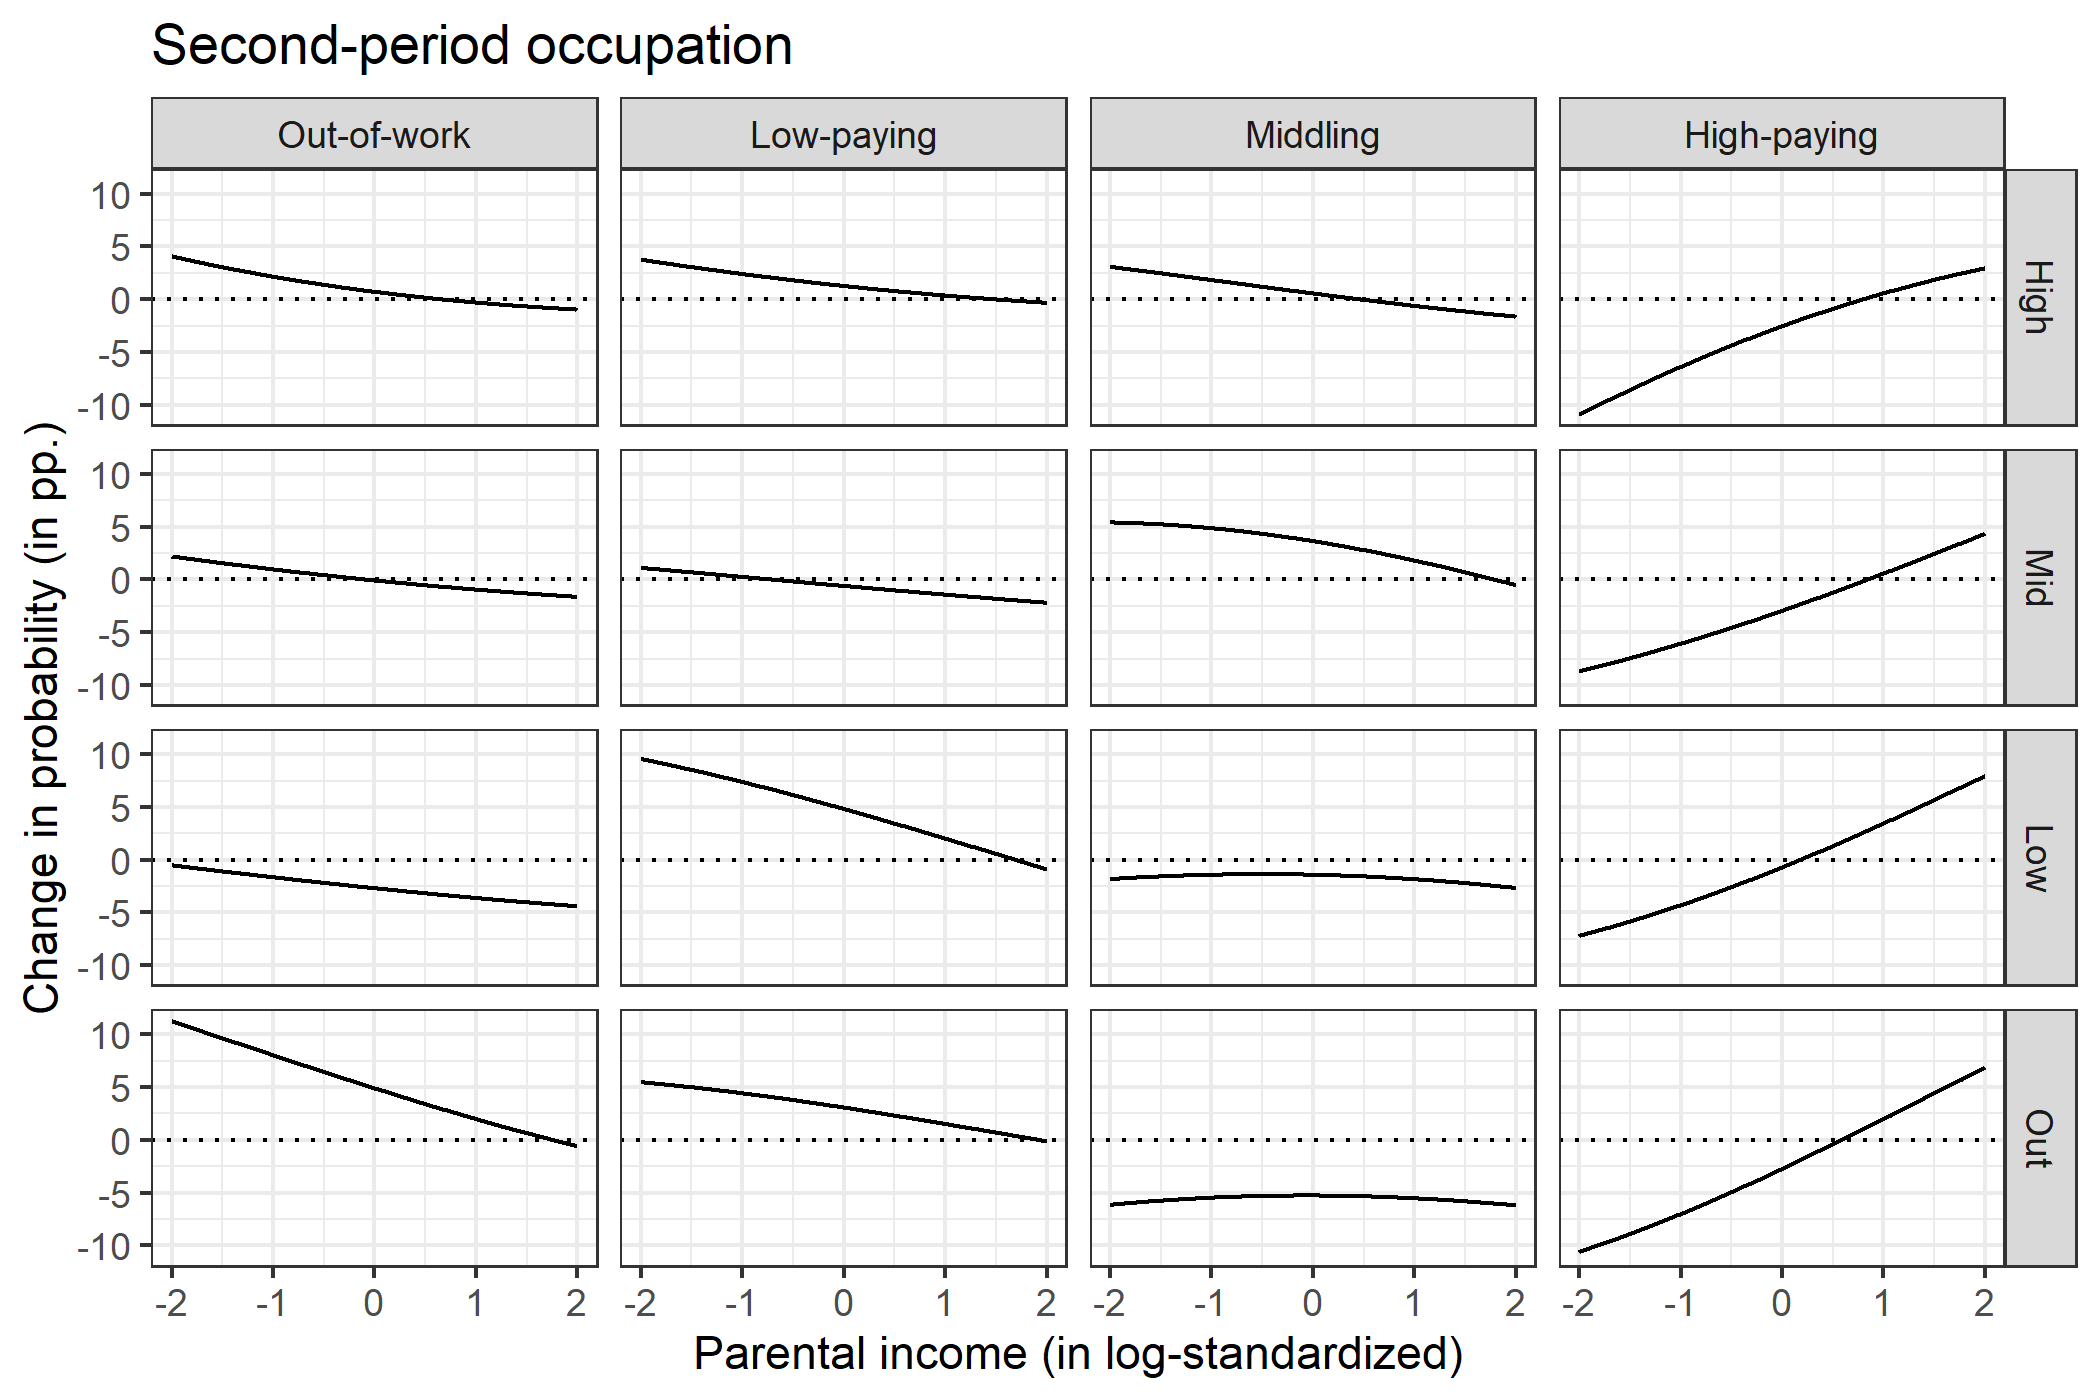
\includegraphics[width=\linewidth]{chap2/graphic/occ-multi3-pinc-male.png}
    \vspace{-3em}
    \justify\singlespacing\footnotesize{\textit{Notes:} This figure presents the difference, expressed in percentage points, between the BCS70 and the NCDS58 cohorts in terms of probability of being in each type of second-period occupation (out-of-work, low-paying, middling, high-paying), conditional on the first-period occupation, according to parental income, in log-standardized.
    Probabilities are computed for males in both cohorts according to the multinomial logistic regression reported in columns (2) of Table \ref{chap2-tab:occ-multi23-base}}
\end{figure}
Each panel represents the gap across cohorts in a particular transition probability for various levels of (standardized) parental income, with positive values implying that the younger cohort has a greater probability of moving from occupation $j$ to occupation $k$, and vice versa. The reported changes are those for men, with the equivalent figure for women provided in appendix \ref{chap2-app-additional}---see Figure \ref{chap2-fig:occ-multi3-pinc-female}.

Consider first individuals at the mean of the distribution. The probability of being in a middling occupation in late career has increased by almost 3.7 pp. for those who started in such occupation but declined for those starting in low-paying occupations or out of work. This indicates a reduction in upwards mobility for those starting in the least well-paid categories. For example, for those who were initially out-of-work, the probability of remaining there has increased by 4.92 pp., and although the probability of being in a high-paying occupation at 42 has slightly increased (by 0.71 pp.), this has occurred at the expense of a large decline in the likelihood of moving into low-paying or middling jobs. The fourth column of graphs, reporting changes in the probability of being in a high-paying occupation, indicates that---for those with mean parental income---the probability of being in such an occupation has fallen irrespective of the initial job. The change is small for those starting in low-paying occupations (-0.71 pp.) but larger for the other three initial occupations, with values between -2.5 and -2.9 pp. This is a surprising finding given that the share of such jobs rose by 5.4 pp.

These changes hide large differences depending on parental background. Consider the changes in the probability of being in a high-paying occupation across cohorts. For those at the top and the bottom of the parental income distribution the changes are large and of opposite sign. Notably, for those who came from a household with parental income 2-standard-deviations below the mean there is a reduction in the probability of attaining the top occupations, irrespective of the initial occupation, which is of considerable magnitude, between 7.2 and 11 pp.. Note that even those who started in high-paying occupations are now less likely to remain there if parental income is low. In contrast, when parental income is 2-standard-deviations above the mean, there is an increase in the likelihood of remaining in or moving to the top, with those who started in a low-paying occupation experiencing a particularly large increase, by 8 pp. 

The second important pattern observed in the data is a dichotomy that appears for those who started in a low-paying occupation. Their probability of moving to a middling occupation has fallen, but the alternative outcome depends on parental income. For those at the bottom of the distribution, the likelihood of remaining in a low-paying occupation has increased (by  4.8 pp. for those with average parental income and by 9.6 pp. for those at -2 standard deviations). In contrast, for those at the top of the parental income distribution the decline in mobility into middling jobs has been accompanied by a greater probability of moving into a high-paying occupation. The natural progression in which individuals would move from low-paying into middling occupations as their careers evolved seems to have weakened, and has been replaced by higher probabilities of either staying in the occupation of origin or jumping up to a high-paying one, with the transition probabilities being strongly dependent on parental income. An equivalent pattern is found when considering those who started in middling occupations, with those at the top (bottom) of the parental income distribution being more likely to be in high-paying (low-paying) jobs in the younger than in the older cohort. 

\subsection{Intra-generational mobility and parental income}

In order to provide a compact measure of mobility, we define three possible outcomes for the second period. Downward mobility is defined as ending up in a category with lower average pay than the individual's initial category; persistence consists of remaining in the same category, and upwards mobility occurs when the individual moves to a category with higher average pay. Hence for those starting in a low-paying occupation, downward mobility occurs if they are out-of-work at age 42, and upwards mobility if they are in a middling or high-paying occupation. 

The upwards/downwards intra-generational mobility measures are depicted graphically in Figure \ref{chap2-fig:persist-both}, in which we plot the \emph{change} in the three probabilities (of moving up, remaining in, and moving down with respect to the initial occupation) for different deciles of the parental income distribution; see also Table \ref{chap2-tab:mob-pinc-both} in the appendix.
\begin{figure}[!tb]
    \centering
    \caption{Change in intra-generational mobility across cohorts}
    \label{chap2-fig:persist-both}
    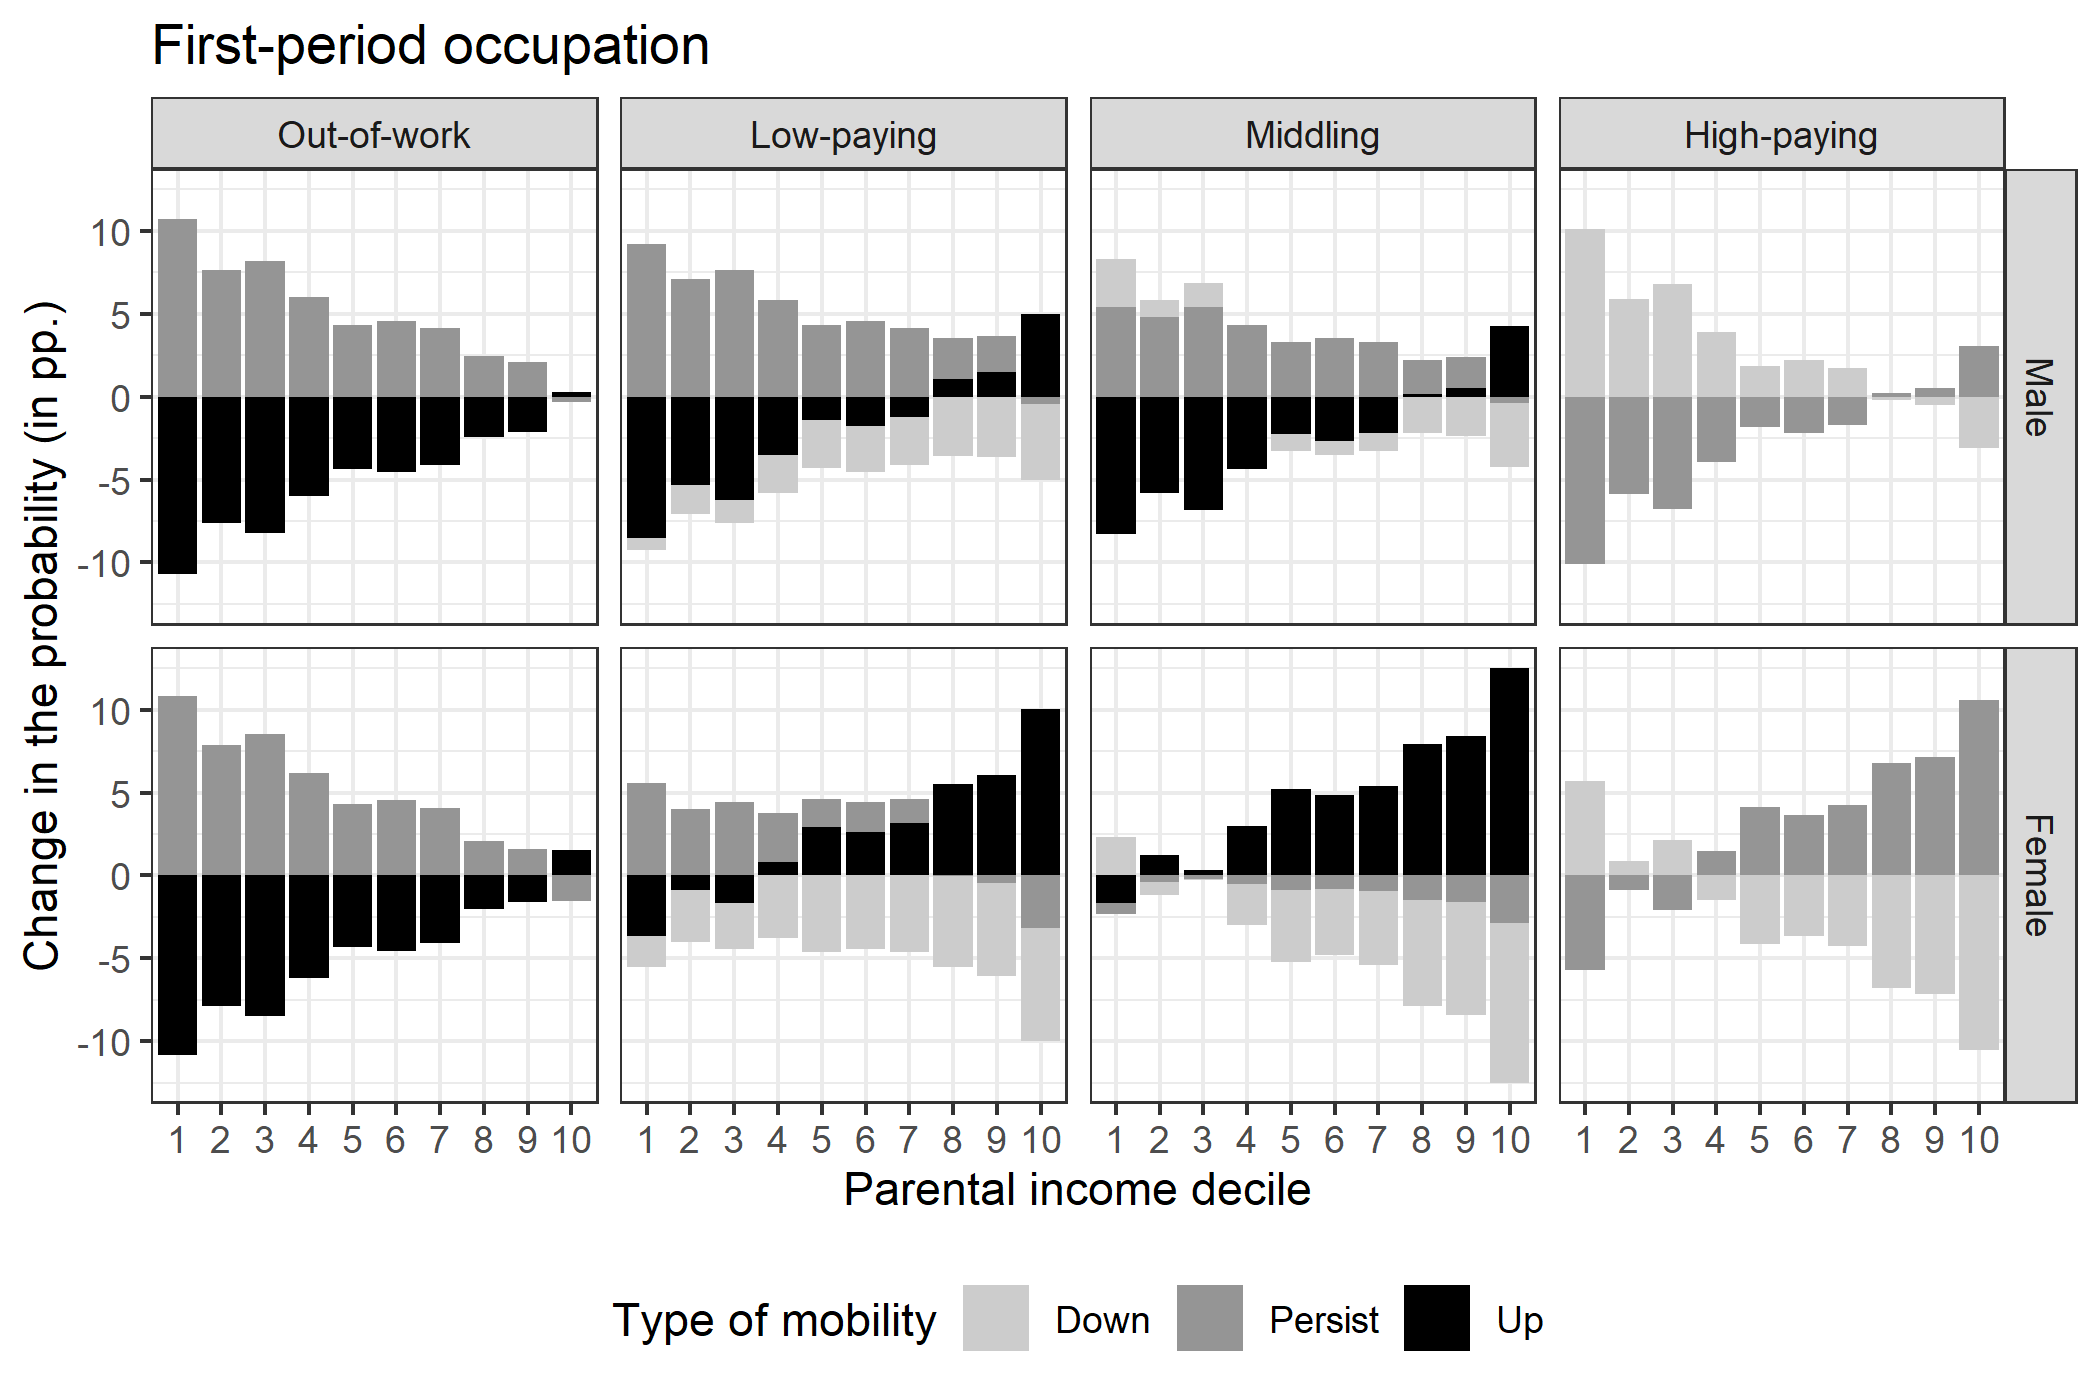
\includegraphics[width=\linewidth]{chap2/graphic/persist-both.png}
    \vspace{-3em}
    \justify\singlespacing\footnotesize{\textit{Notes:} This figure presents the difference, expressed in percentage points, between the BCS70 and the NCDS58 cohorts in terms of type of mobility (down, persist, up) conditional on the first period occupation (out-of-work, low-paying, middling, high-paying) according to the decile of the parental income distribution.
    Probabilities are computed for males and females at each parental income decile, according to the multinomial logistic regression reported in columns (2) of Table \ref{chap2-tab:occ-multi23-base} in the appendix.}
\end{figure}

Consider first those who started in high-paying occupations. The two possible occupational dynamics are to move downwards (depicted in light grey) or to remain in a high-paying occupation (depicted in dark grey). Those born to parents in the top decile are 3 pp. more likely to stay in that occupation and 3 pp. less likely to move into a lower-income occupation in the 1970 cohort than those born in 1958. The reverse effect appears for those at the bottom of the parental income distribution, with those in the bottom decile being 10 pp. more (less) likely to experience downwards mobility (remain in the occupation). The reduction in persistence falls as we move up the parental income distribution, with the sign reversing for the 9th and 10th deciles. The figure displays what we could call a \emph{polarization of mobility}, whereby for those in the middle of the distribution there have been only moderate changes in mobility, while at the extreme the changes have been large, although in opposite directions for those at the bottom and at the top. 

An equivalent pattern is observed for those that start their careers in middling occupations. Those at the bottom of the parental distribution witnessed sharp declines in upwards mobility and higher persistence and likelihood of moving down, with the size of the changes declining as we move along the income distribution. The pattern is reversed from the 8th decile, with the likelihood of moving upwards increasing across cohorts for the top three deciles. The polarization of mobility is also apparent for those starting in low-paying occupations for whom the probability of moving into middling or high-paying occupations increases only for the top three deciles. Lastly, for those initially out-of-work, only those in the top decile of the parental income distribution witness an increase in the likelihood of upwards mobility. Note that for those in the bottom decile the magnitudes of the change are large: the probability of staying has increased by 10 pp., which is offset by an equivalent decline in the probability of moving upwards. Overall these results indicate that the change in the structure of employment has been accompanied by a polarization of intra-generational mobility, with the probabilities of moving across occupations changing in opposite directions depending on whether individuals had parents at the top or at the bottom of the income distribution.

Not surprisingly, the dynamics for women differ considerably from those for men, as women of the older cohort where much less likely to occupy middling and especially high-paying occupations. The bottom panels of Figure \ref{chap2-fig:persist-both} capture, however, the advantage that parental income gives in providing the means for upwards mobility. Irrespective of parental income, women starting in a high-paying occupation (resp. middling) have a greater probability of remaining there (moving upwards) for the younger cohort. This is not surprising in view of the occupational upgrading experienced by women of the younger cohort. In contrast, for those who started in low-paying occupations, a polarization appears, although the turning point occurs for lower parental incomes than in the case of men (4th decile), indicating the tension between the general occupational upgrading of women and the decline in mobility observed for workers coming from a less well-off background. The results for those out of work broadly mimic those for men. Overall, despite the differences due to women's increased access to all occupations, these figures confirm the increased importance of parental income for intra-generational mobility.


    
    \section{Mobility and polarization at the regional level}\label{chap2-regional}
    \subsection{Regional polarization}

The geography of mobility has received considerable attention over the past few years,\footnote{See \cite{Chetty2014Land} and \cite{Bell2018Land} amongst others.} and in this section we turn to exploring the regional dimension of our data. We focus on two aspects, both of which address the hypothesis that the observed increase in the impact of parental income on occupational outcomes is related to the polarization of employment. The next subsection considers whether the reduction in mobility that we have identified appears when we replace the cohort dummies by a measure of the extent of polarization that individuals faced in their region when they were young. It hence asks if the cohort dummies are capturing the differences in the structure of the labour market over time. Our second strategy consists in estimating the impact of parental income on occupational outcomes at the regional level in order to get regional measures of mobility. We then ask whether there is a correlation between the changes over time in regional mobility and the increase in polarization at the local level.

Our data have information on 10 regions and hence do not allow us to identity the very local effects that other work has observed.\footnote{\cite{Chetty2014Land} focus on considerably smaller locations in their analysis for the US. For the UK, \cite{Bell2018Land} consider a dataset with the 32 NUTS2 regions but which does not have information on parental income.} For both analyses we need to construct a measure of polarization at the regional level, but we are impaired by the fact that sample sizes at the regional level are small and thus measures of regional polarization based on our cohort data may not capture well the actual changes in the structure of employment. In order to have a more representative sample we use data from the Labour Force Survey (LFS) to build polarization measures. 

When computing the extent of polarization we face two concerns. First, as shown in the appendix, the share of middling employment has fallen in all regions, but whether this has occurred at the expense of low-paying or high-paying occupations varies. For this reason, rather than focusing exclusively on the share of middling jobs we consider changes in the share of jobs in all three occupations. Second, we need to define the job market that individuals in our dataset were facing and measure the extent of polarization in that particular market. To do so we consider the distribution of employment for the relevant age cohorts in the LFS. We hence suppose that members of a cohort are in competition for jobs with individuals that were born in the 5 years before and 5 years after them. That is, for the NCDS58 cohort we consider individuals born between 1953 and 1963, and for the BCS70 those born between 1965 and 1975. We measure the share of employment in each year between the initial and final period that we use for each cohort, and compute the average over the whole period in which each cohort has been exposed to employment changes. That is, for the NCD58 we consider the structure of employment between 1981 and 2000, for the BCS70 between 1996 and 2012. We then measure the extent of polarization as changes in the occupational shares obtained for the 1953-63 cohorts and those for the 1965-75 ones. Appendix \ref{chap2-app-data-LFS} gives details on the LFS data and our measures of polarization, and shows that all regions exhibited an increase in polarization (see Figure \ref{chap2-fig:lfs-change}).


\subsection{Individual outcomes and regional employment patterns}

Several factors may be behind the increased importance of parental income for occupational outcomes across cohorts. Here we explore the possibility that employment polarization is one of these factors. To do so, we substitute the cohort dummy used in our regressions by our measure of regional polarization. We use the region in which the individual lived at age 16, and measure polarization in that region as the share of middling employment in the year in which the individuals are 23/26.

Table \ref{chap2-tab:regocc-multi2A-short} displays the results obtained from the multinomial regression, regression, with the first three columns reporting again the estimates when we use the cohort dummies (i.e. those in Table \ref{chap2-tab:occ-multi2-short} above), and the last three columns those in which we substitute the dummies for the share of non-middling jobs and this share interacted with parental income (both standardized). The regressions also include a region fixed effect. We focus on the effect of the share of non-middling employment as an increase in its value can be interpreted as an increase in polarization. \footnote{Results using jointly the low- and high-paying employment shares are reported in Table \ref{chap2-tab:regocc-multi2B-short} in the appendix. We also used alternative measures of polarization using data on only the initial year measure of polarization for each cohort (1981 and 1996) rather than the average over the working-life and found equivalent results to those reported here (results not reported).} 
\begin{table}[!tb]
    \centering
    \caption{Second-period occupation probability according to share of non-middling occupations in the region at the age 16}
    \label{chap2-tab:regocc-multi2A-short}
    \resizebox*{\textwidth}{!}{
    \begin{threeparttable}
        \setlength{\tabcolsep}{0pt}
        \begin{tabular}{l D{.}{.}{5.3} D{.}{.}{5.5} D{.}{.}{5.5} D{.}{.}{5.3} D{.}{.}{5.5} D{.}{.}{5.5}}
\toprule
 & \multicolumn{6}{c}{Multinomial logit - Dep. var.: Second-period occupation} \\
\cmidrule(lr){2-7}
 & \multicolumn{3}{c}{(1)} & \multicolumn{3}{c}{(2)} \\
\cmidrule(lr){2-4}\cmidrule(lr){5-7}
 & \multicolumn{1}{c}{Low} & \multicolumn{1}{c}{Mid} & \multicolumn{1}{c}{High} & \multicolumn{1}{c}{Low} & \multicolumn{1}{c}{Mid} & \multicolumn{1}{c}{High} \\
\midrule
BCS cohort                        & 0.05   & -0.03      & 0.11       &        &            &            \\
                                  & (0.11) & (0.09)     & (0.09)     &        &            &            \\
Non-Middling share                &        &            &            & 0.07   & 0.02       & 0.17^{***} \\
                                  &        &            &            & (0.06) & (0.05)     & (0.05)     \\
Parental income                   & 0.01   & 0.04       & 0.19^{***} & 0.04   & 0.11^{***} & 0.35^{***} \\
                                  & (0.04) & (0.04)     & (0.04)     & (0.03) & (0.03)     & (0.03)     \\
Par. inc. $\times$ BCS            & 0.05   & 0.16^{***} & 0.36^{***} &        &            &            \\
                                  & (0.06) & (0.05)     & (0.05)     &        &            &            \\
Par. inc. $\times$ Non-Mid. share &        &            &            & -0.00  & 0.04^{*}   & 0.11^{***} \\
                                  &        &            &            & (0.03) & (0.02)     & (0.02)     \\
\midrule
Num. obs. & \multicolumn{1}{c}{14763} & \multicolumn{1}{c}{14763} & \multicolumn{1}{c}{14763} & \multicolumn{1}{c}{14763} & \multicolumn{1}{c}{14763} & \multicolumn{1}{c}{14763}\\
\bottomrule
\end{tabular}

        \begin{tablenotes}[flushleft]
            \footnotesize{\item\textit{Notes}: 
            % Stars and SE
            $^{***}p<0.01$; $^{**}p<0.05$; $^{*}p<0.1$. Standard errors between parentheses. 
            % Baseline outcome
            Out-of-work occupation in second period is the base outcome of the multinomial logistic regression.
            % Referent group
            Male in the NCDS58 cohort is the referent group in (1), while male is the referent group in (2).
            % Variables details
            Parental income in logarithm and then standardized at the cohort level. 
            Non-middling share corresponds to the share of occupations that are not middling, hence, low-paying and high-paying, in total employment in the region at age 16. The shares has been standardized for the interpretability of coefficients when interacted with parental income.
            % Control variables
            Control variables in (1) include Intercept, Female and Female $\times$ BCS, while control variables in (2) include Intercept, Female and Female $\times$ Non-Mid. share. %; see Table \ref{chap2-tab:tobefilled} in the appendix for these coefficients.
            }
        \end{tablenotes}
    \end{threeparttable}
    }
\end{table}

The coefficients of interest have the expected sign. A higher share of non-middling employment is associated with a greater average probability of being in a high-paying occupation, as we would expect given the greater availability of these jobs. There is no significant effect on the other employment categories, implying that higher polarization does not affect the allocation of workers between out-of-work, low-paying jobs and middling jobs. Parental income has, as expected, a positive impact on the likelihood to be in middling and high-paying jobs, and the interaction terms indicate that as polarization increases the effect of background becomes stronger. To gauge the magnitude of these effects, we average the (standardized) share of middling employment across regions for each cohort, obtaining that for the NCDS58 (resp. BCS70) it is 0.845 standard deviations below (above) the mean. Using these figures, the coefficients on column (6) imply that a one standard deviation increase in parental income raised the probability of being in a high-paying occupation by 0.14 pp. for the older cohort and by 0.44 for the younger one. These values are close to those obtained in our core specification (column (3)) of 0.19 and 0.55, indicating that using the differences in polarization across cohorts yield effects that are close to those obtained with the cohort dummy. 


\subsection{Regional mobility} 

Our final step consists in exploiting the cross-sectional variation in the regional data to consider the correlation between regional mobility and polarization. We start by running the same multinomial regressions as in equation \ref{chap2-eq:emp-multi3} but at the regional level.\footnote{We do not compute first-period mobility and conditional second-period mobility because of sample sizes, as in many regions we have only a small number of individuals moving across certain occupations between first and second period.} Table \ref{chap2-tab:reg-multi2-short} presents the coefficients on parental income obtained when we regress second period occupation on parental income. As before, we need to recall that these are the coefficients relative to the probability of being out-of-work (see also Figures \ref{chap2-fig:reg-multi2-pinc-male} and \ref{chap2-fig:reg-multi2-pinc-female} in the appendix).

\begin{table}[!tb]
    \centering
    \caption{Probability of second-period occupation by region}
    \label{chap2-tab:reg-multi2-short}
    \resizebox*{!}{\dimexpr\textheight-2\baselineskip\relax}{
    \begin{threeparttable}
        \centering
        \setlength{\tabcolsep}{12pt}
        \begin{tabular}{l D{.}{.}{3.5} D{.}{.}{3.5} D{.}{.}{3.5}}
\toprule
 & \multicolumn{3}{c}{Multi. logit - Dep. var.: Second-period occupation} \\
\cmidrule(lr){2-4}
 & \multicolumn{1}{c}{Low-paying} & \multicolumn{1}{c}{Middling} & \multicolumn{1}{c}{High-paying} \\
\midrule
\midrule
 East Anglia (N = 904) & & & \\
\midrule
Par. inc.              & 0.04       & -0.00       & 0.13        \\
                       & (0.15)     & (0.14)      & (0.14)      \\
Par. inc. $\times$ BCS & -0.10      & 0.31        & 0.57^{**}   \\
                       & (0.25)     & (0.26)      & (0.26)      \\
\midrule
 East Midlands (N = 1066) & & & \\
\midrule
Par. inc.              & 0.06       & 0.12        & 0.17        \\
                       & (0.15)     & (0.15)      & (0.15)      \\
Par. inc. $\times$ BCS & 0.45^{**}  & 0.44^{**}   & 0.92^{***}  \\
                       & (0.22)     & (0.21)      & (0.21)      \\
\midrule
 North (N = 1037) & & & \\
\midrule
Par. inc.              & -0.04  & -0.08       & 0.02        \\
                       & (0.15) & (0.14)      & (0.14)      \\
Par. inc. $\times$ BCS & 0.07   & 0.34        & 0.58^{***}  \\
                       & (0.22) & (0.22)      & (0.21)      \\
\midrule
 North West (N = 1810) & & & \\
\midrule
Par. inc.              & 0.12       & 0.06        & 0.32^{***}  \\
                       & (0.11)     & (0.10)      & (0.11)      \\
Par. inc. $\times$ BCS & -0.01      & 0.32^{**}   & 0.35^{**}   \\
                       & (0.16)     & (0.15)      & (0.15)      \\
\midrule
 Scotland (N = 1489) & & & \\
\midrule
Par. inc.              & 0.03   & 0.13        & 0.14        \\
                       & (0.12) & (0.12)      & (0.12)      \\
Par. inc. $\times$ BCS & 0.18   & 0.17        & 0.52^{***}  \\
                       & (0.18) & (0.18)      & (0.17)      \\
\midrule
 South East (N = 3718) & & & \\
\midrule
Par. inc.              & 0.01       & 0.06        & 0.17^{**}   \\
                       & (0.09)     & (0.08)      & (0.08)      \\
Par. inc. $\times$ BCS & -0.06      & 0.02        & 0.26^{**}   \\
                       & (0.11)     & (0.11)      & (0.11)      \\
\midrule
 South West (N = 1141) & & & \\
\midrule
Par. inc.              & -0.10      & 0.05        & 0.17        \\
                       & (0.16)     & (0.16)      & (0.16)      \\
Par. inc. $\times$ BCS & 0.08       & -0.02       & 0.31        \\
                       & (0.21)     & (0.21)      & (0.21)      \\
\midrule
 Wales (N = 821) & & & \\
\midrule
Par. inc.              & -0.23  & -0.16       & -0.07      \\
                       & (0.17) & (0.16)      & (0.16)     \\
Par. inc. $\times$ BCS & 0.34   & 0.27        & 0.62^{***} \\
                       & (0.24) & (0.23)      & (0.22)     \\
\midrule
 West Midlands (N = 1495) & & & \\
\midrule
Par. inc.              & 0.04   & 0.12        & 0.63^{***}  \\
                       & (0.12) & (0.12)      & (0.14)      \\
Par. inc. $\times$ BCS & 0.09   & 0.12        & -0.08       \\
                       & (0.17) & (0.17)      & (0.18)      \\
\midrule
 Yorkshire and Humberside (N = 1282) & & & \\
\midrule
Par. inc.              & 0.03   & -0.05       & 0.02        \\
                       & (0.14) & (0.12)      & (0.12)      \\
Par. inc. $\times$ BCS & 0.06   & 0.21        & 0.53^{***}  \\
                       & (0.19) & (0.17)      & (0.17)      \\
\bottomrule
\end{tabular}

        \begin{tablenotes}[flushleft]
            \footnotesize{\item \textit{Notes}: 
            % Stars and SE
            $^{***}p<0.01$; $^{**}p<0.05$; $^{*}p<0.1$. Standard errors between parentheses. 
            % Baseline outcome
            Out-of-work occupation in second period is the base outcome of the multinomial logistic regression.
            % Referent group
            Male in the NCDS58 cohort is the referent group.
            % Variables details
            Parental income in logarithm and then standardized at the cohort level.
            % Control variables
            Control variables in all regressions include Intercept, BCS cohort, Female and Female $\times$ BCS.}
        \end{tablenotes}
    \end{threeparttable}
    }
\end{table}

These regressions allow us to make two inferences. First, we can ask whether the changes in occupational mobility observed across cohorts at the national level also took place at the regional level and are not the result of the population reallocating across regions with different mobility patterns. When we split the data we find that for the vast majority of regions (7/10) parental income exhibits insignificant coefficients for the older cohort. Only in the North West, the South East and the West Midlands do we find a significant coefficient on parental income. Note, however, that out of the seven regions for which the coefficient is not significant, 4 of them have magnitudes close to the 0.19 point estimate we obtained at the national level. The lack of significance can then be due to a lack of statistical power given the limited number of observations (per region and also in certain region-occupation cells). For those born in 1970, the likelihood to be in a high-paying occupation exhibits systematically large and significant coefficients on parental income. Out of the 10 regions only two (South West and West Midlands) do not display a significant coefficient. In all the others, the magnitude of the effect is large, with the coefficient being at least twice as large for the younger as for the older cohort (eg. North West) and much larger in others. These results indicate that the increase in the importance of parental income across cohorts holds at the regional level.

Second, the estimates imply large variations in the degree of inter-generational income mobility across locations, with the probability of someone born in a household in the bottom quintile moving to the top quintile being three times higher in the most than in the least mobile locations. This raises the question of whether the magnitude of the changes in mobility is correlated to the degree of employment polarization observed at the regional level. 

To capture changes in mobility in region $r$, we consider the between-cohort change in the role of parental income for being in a high-paying occupation, namely, $\Delta\beta_H^r$. These coefficients correspond to the ``$\text{Par. Inc. }\times\text{ BCS}$'' coefficients in Table \ref{chap2-tab:reg-multi2-short}. The change in the extent of regional polarization is measured by the change across cohorts in regional polarization as measured from the LFS. Figure \ref{chap2-fig:regocc-absolute-high} displays the correlation between the two variables, with both measured in percentage points. The three panels report, in the horizontal axis, the changes in absolute value of the share of employment in each of the three categories. The actual changes are positive for high- and low-paying occupations and negative for middling ones, hence reporting the absolute value implies that for all three occupational categories moving from the left to the right of each graph implies an increase in polarization. The vertical axis displays the regional $\Delta\beta_{H}$ described above.
\begin{figure}[!tb]
    \centering
    \caption{Change in parental income coefficient for high-paying second-period occupation according to job polarization at the regional level}
    \label{chap2-fig:regocc-absolute-high}
    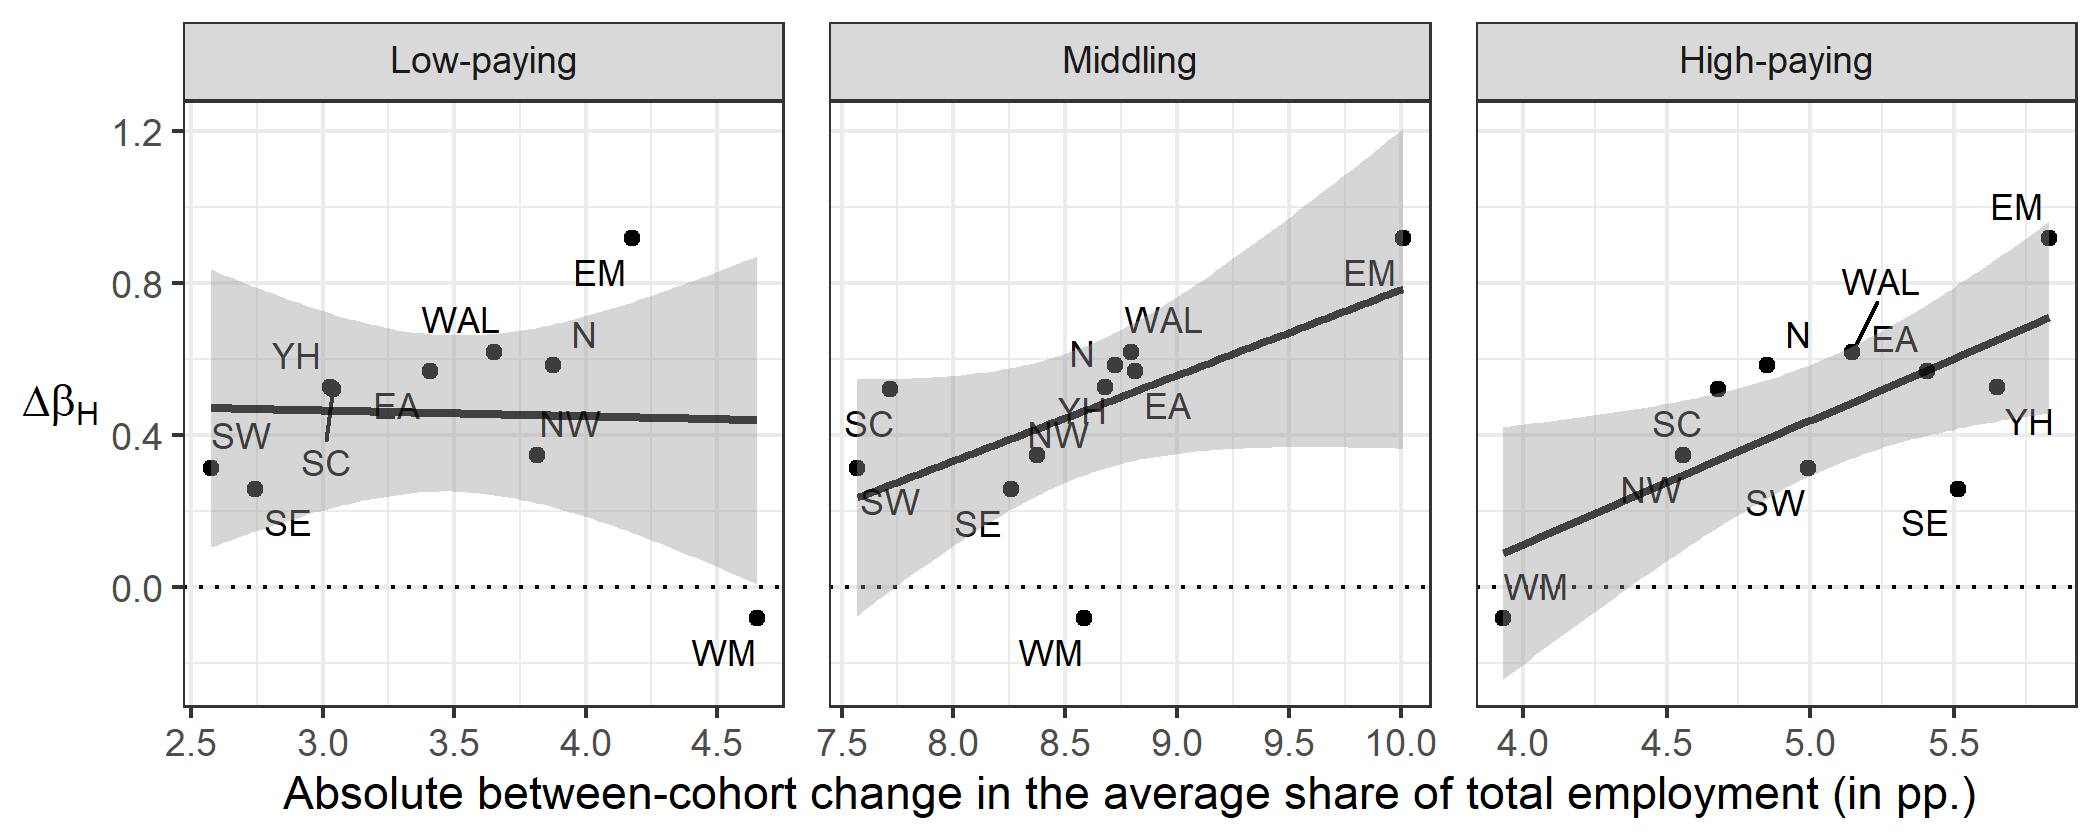
\includegraphics[width=\linewidth]{chap2/graphic/regocc-absolute-high.png}
    \vspace{-3em}
	\justify\singlespacing\footnotesize{\textit{Notes:} This figure presents the correlation across regions between the change in the parental income coefficient for the high-paying occupation in second period $\Delta\beta_H$ and the between-cohort change in absolute value in the average share of total employment of low-paying, middling, and high-paying occupations, in percentage points. Note that, by taking the absolute value of the change, we reversed the x-axis for the middling panels (middle column). Thus, regions on the left-hand (resp. right-hand) side of each panel are those where the polarization of employment has been lower (resp. larger).}
\end{figure}

Each dot represents one of the 10 regions, while the line corresponds to the linear regression line.\footnote{Figure \ref{chap2-fig:regocc-absolute-all} in the appendix presents equivalent graphs for the change in the coefficients on parental income in the probability of being in middling and low-paying occupations, namely, $\Delta\beta_{M}$ and $\Delta\beta_{L}$. We obtain broadly similar results in the two cases,} Consider the right-most graph. The upward slope indicates that regions where the share of high-paying occupations (in the relevant age group) increased the most are also the regions where the impact of parental income in accessing high-paying occupations rose the most. Similarly, the middle graph also displays an upwards-slopping schedule when we plot the magnitude of the change in the share of middling occupations against $\Delta\beta_{H}$, indicating that regions where the share of middling income jobs declined the most are also those where parental impact became strongest. The left-hand graph depicts the correlation between the change in the coefficient and the change in the share of low-paying occupations, and displays a flat schedule, which is driven by an outlier, the West-Midlands. Removing this observation, yields a positive correlation between the change in polarization and the change in the effect of parental income.

This subsection, together with the previous one, provide suggestive evidence that the increase in employment polarization may be a cause of the reduction in occupational mobility observed across the two cohorts. When we exploit the time dimension, we find that differences in the extent of polarization experienced by the two cohorts result in estimates of the impact of parental income that are close to those obtained when using cohort dummies. The cross-sectional evidence, in turn, indicates that when we estimate mobility measures by regions, the increases in \emph{immobility} that we observe are correlated with regional increases in polarization.





    
    \section{Conclusion} \label{chap2-conclusion}
    A vast literature has discussed the consequences of job polarization for wage inequality. In contrast, little is known about whether the change in the employment structure has also had an impact on social mobility. This paper raises such question using British data for two cohorts for which we have information for parents and children.

We start by developing a simple theoretical setup with three types of jobs and two levels of parental income. Parental background will affect the child's human capital so that the latter’s productivity is determined both by human capital and innate (and initially unobservable) ability. Children’s entry jobs will be determined by parental background, but as their ability is revealed, they may move up or down the occupational ladder. As the share of middle jobs disappears, the possibilities for mobility fall, thus leading to greater job persistence across generations.

The model highlights not only the importance of polarization for social mobility, but also the fact that transitions across occupations---i.e. intra-generational occupational dynamics---are an essential aspect of inter-generational mobility. Our empirical approach uses data on two British cohorts that are particularly suited for our purposes. First, the two cohorts, born 12  years apart, entered the labour market under substantially different conditions in terms of the structure of employment, with the latter cohort facing a much more polarized labour market. Second, we have data for children at various ages so that we can identify to what extent upwards mobility is driven by an improvement in the occupation at which children enter the labour market or by them going up the occupational ladder during their work-life. 

The data indicate that intra-generational occupational changes are an important source of mobility, with large shares of those starting in low-paying and middling occupations moving, respectively, to middling and high-paying jobs over their work lives. When we compare the two cohorts, we find that as the share of middling jobs has fallen these two sources of occupational mobility have weakened. Our results indicate that the role of parental income in determining occupations has increased, both for first-period occupations and for the transition towards better-paid occupations. For example, the fortunes of those who start in low-paying jobs differ considerably across generations. For the older cohort, a considerable fraction moved into middling jobs, but this probability has fallen markedly for the younger cohort. At the same time, the probability for those who start in low-paying jobs to move into high-paying jobs has remained roughly stable on average, but this average hides the fact that it has considerably increased for those with high-income parents and declined for those from low-income backgrounds. 

Although our data does not allow us to establish causality, the changes we identify are suggestive that as middling jobs have been eroded, parental income has become more important in determining occupational outcomes. Our analysis of regional mobility patterns finds that regions where employment polarization rose the most are also those where \emph{immobility} increased the most. These results hence suggest that the structure of employment affects not only the distribution of earnings but also the degree of occupational mobility. Moreover, they point towards the possibility that there is a transmission of polarization across generations, and that the increased importance of parental background may accumulate across generations creating a multiplier effect that over time accentuates the occupational distance across groups from different backgrounds. This is a question that we intend to pursue in future work. 
    
    \printbibliography[heading=subbibintoc]
    
    \clearpage
    \addsec{Appendices}
    \renewcommand{\thesubsection}{\thechapter.\Alph{subsection}}
    
    \subsection{Model derivations}\label{chap2-app-model}
    This appendix presents details on the model.

\subsubsection{The allocation of labour under imperfect information}

Under imperfect information, the second-period distribution of expected skills is given by
\begin{equation*}
    h=\left\{ 
    \begin{array}{cc}
    \underline{h}_{L} & (1-\pi )(z_{L}-q_1) \\ 
    \widehat{h}_L & q_{1} \\ 
    \underline{h}_{H} & (1-\pi )z_{H} \\ 
    \overline{h}_{L} & \pi (z_{L}-q_1) \\ 
    \overline{h}_{H} & \pi z_{H}%
    \end{array}%
    \right.  
\end{equation*}

Let $d_{1,2}$ (resp. $d_{2,3}$) be the threshold productivity between low-paying and middling jobs (resp. middling and high-paying jobs), i.e. $d_{1,2}$ is the skill for which individuals below this level are assigned to job type $1$. By construction, we have that $d_{1,2} \leq d_{2,3}$. Various scenarii are possible, and we focus on the case where low-paying jobs are filled with individuals from low-skill households, while middling and high-paying jobs contain workers from both low- and high-skill households. Assumption \ref{chap2-ass:threshold-skill-p2} ensures that this is the case. 

Under assumptions \ref{chap2-ass:threshold-skill-p1} and \ref{chap2-ass:threshold-skill-p2}, the
probability that an individual with parental background $i=\{L,H\}$ is in occupation $k\in\{1,2,3\}$ when mature, namely $P_j(k)$, is given by
\begin{align*}
    P_L(1) &=\frac{q_1}{z_L}, &&P_H(1) = 0,\\
    P_L(2) &=(1-\pi)\left(1-\frac{q_1}{z_L}\right), &&P_H(2) = 1- \pi - \frac{q_{3}-\pi (1-q_{1})}{z_{H}},\\
    P_L(3) &=\pi \left(1-\frac{q_1}{z_L}\right), &&P_H(3) = \pi +\frac{q_{3}-\pi (1-q_{1})}{z_{H}}.
\end{align*}
Note that Assumption \ref{chap2-ass:threshold-skill-p2} above imply that $q_{3}-\pi (1-q_{1})>0$. 

We can now consider how changes in $q_{1}$ and $q_{3}$ (at the expense of $q_{2}$) affect inter-generational mobility. As long as Assumptions \ref{chap2-ass:threshold-skill-p1} and \ref{chap2-ass:threshold-skill-p2} hold, we have that
\begin{itemize}
    \item An increase in $q_{1}$ increases the probability of being in occupation 1 and reduces those of being in occupations 2 and 3 for individuals from low-income households. For individuals from high-income households, it increases the probability of being in occupation 3 and reduces that of being in occupation 2.
    \item An increase in $q_{3}$ has no effect on the probabilities for individuals from low-skilled households. For individuals from high-income households, it increases the probability of being in occupation 3 and reduces that of being in occupation 2.
\end{itemize}

\subsubsection{The occupation distribution of mature workers under perfect information }

In this subsection we consider the way in which our assumption about the information content of occupations affects mobility. We compare the distribution of occupations obtained under this assumption with that in the case in which there is perfect information. Under perfect information, firms face a distribution of skills in which they know for all workers whether they are high or low ability as well as their family type. The distribution of observed second-period skills is then
\begin{equation*}
    h=\left\{ 
    \begin{array}{cc}
        \underline{h}_{L} & (1-\pi )z_{L} \\ 
        \underline{h}_{H} & (1-\pi )z_{H} \\ 
        \overline{h}_{L} & \pi z_{L} \\ 
        \overline{h}_{H} & \pi z_{H}%
    \end{array}%
    \right.  
\end{equation*}

Under assumptions \ref{chap2-ass:threshold-skill-p1} and \ref{chap2-ass:threshold-skill-p2}, the
probability that an individual with parental background $i=\{L,H\}$ is in occupation $k\in\{1,2,3\}$ when mature, namely $P^\prime_i(k)$, is given by
\begin{align*}
    P^\prime_L(1) &=\frac{q_1}{z_L}, &&P^\prime_H(1) = 0,\\
    P^\prime_L(2) &=1-\frac{q_1+q_3}{z_{L}}, &&P^\prime_H(2) = 1-\pi,\\
    P^\prime_L(3) &=\frac{q_{3}-\pi (1-z_{L})}{z_{L}}, &&P^\prime_H(3) = \pi.
\end{align*}
These expressions imply that for those born in high-income households, the probabilities of being in the various occupations are independent of the distribution of employment. For those born in low-income households, both $q_1$ and $q_3$ have an impact. An increase in either of them (i.e. greater polarization) would reduce the share of those born in low-income households that works in middling occupations, thus, increasing the likelihood of being employed in the other two types of jobs. Polarization can hence affect mobility also in the case of perfect information through a direct mechanical effects due to the availability of jobs. Note, however, that in this case there are no inefficiencies associated with the allocation of labour, and that whether those from L-households benefit is ambiguous as both their likelihood of being in high- and low-paying occupations increases.

Comparing these latter probabilities to those in Table \ref{chap2-tab:uncond-prb-p2} and given assumptions \ref{chap2-ass:threshold-skill-p1} and \ref{chap2-ass:threshold-skill-p2}, we can write
\begin{align*}
    P_L(1)-P_L^\prime(1) &= 0, \\
    P_L(2)-P_L^\prime(2) &=\frac{q_{3}-\pi
    (1-q_{1})}{z_{L}}>0, \\
    P_L(3)-P_L^\prime(3) &= -\frac{q_{3}-\pi
    (1-q_{1})}{z_{L}}<0, \\
    P_H(1)-P_H^\prime(1) &= 0, \\
    P_H(2)-P_H^\prime(2) &= -\pi -\frac{q_{3}-\pi(1-q_{1})}{z_{H}}<0, \\
    P_H(3)-P_H^\prime(3) &= \pi +\frac{q_{3}-\pi (1-q_{1})}{z_{H}}>0.
\end{align*}
When comparing to the case with perfect information, the \textit{information friction} implies that:
\begin{itemize}
    \item those who come from worse-off households experience no change in the probabilities of being in low-paying occupations, but a higher (lower) likelihood of being in a middling (high-paying) occupation;
    \item those who come from high-income households experience no change in the probabilities of being in low-paying occupations, but a lower (higher) likelihood of being in a middling (high-paying) occupation.
\end{itemize}
The information friction provides an inefficiency as under the friction we find in occupation 3 individuals that have a lower productivity that some of those in occupation 2, the former being low-ability individuals with high-income parents and the latter high-ability individuals with low-income parents. We can now consider how polarization affects the gaps due to the information friction. An increase in either $q_{1}$, or $q_{3}$, or both, will increase (decrease) the likelihood that individuals from high-income households are in occupation 3 (occupation 2) and decrease (increase) the likelihood that individuals from low-income households are in occupation 3 (occupation 2).

The model then highlights that although polarization will affect the extent of mobility even under perfect information, imperfect information strengthens the effect. Moreover, it creates an inefficiency as some workers occupying high-paying jobs have a lower productivity than certain that are in less well paid jobs, and the extent of this missallocation will be greater the more polarized the distribution of employment is.
    \clearpage
    \subsection{Data and summary statistics}\label{chap2-app-data}
    This appendix presents further details on the data as well as summary statistics, and provides additional tables and figures about the structure of employment and the extent of job polarization observed in the data. 

\subsubsection{Cohort studies}\label{chap2-app-data-cohort}

We start by describing additional variables that will be used in the robustness analysis. 

\textbf{Education.} We observe both child and parental education as time-invariant variables. To define the child education variable, we take the highest academic qualification ever obtained from the educational qualifications history.\footnote{There are 11 categories which are (from the lowest to the highest): no qualifications; less than O-level; less than 5 O-levels; 5+ O-levels; 1 A-level and less than 5 O-levels; 1 A-level and 5+ O-levels; 2+ A-levels and less than 5 O-levels; 2+ A-levels and 5+ O-levels; Sub degrees; Degree - lower grade; Degree - first and upper second grade; and Higher degree.} For parental education such information is not available, hence we use the age at which each parent left full-time education as a proxy. All education variables are ranked at the cohort level in peer-inclusive downward-looking ranking.\footnote{We follow \cite{Cowell2017Inequality} to define the peer-inclusive downward-looking ranking. It corresponds to the rank within the sample of an individual on the variable's dimension divided by the number of individuals in the sample. Peer-inclusive means that when two individuals have the same value for the variable they have the same rank, while downward-looking means that we attribute the value of 1 (respectively, 0) to the individual with the highest (respectively, lowest) value in the sample. An observation with a value of 0.3 means that 30\% of the sample has a lower or equal level of the variable. See, for example, \cite{Jenkins2021Inequality} for an application.} This approach is particularly suited to the period, given the massive expansion of secondary and higher education that occurred between the two cohorts; see Figures \ref{chap2-fig:stat-educ-child-short} and \ref{chap2-fig:stat-educ-parents}.

\textbf{Family characteristics.} A number of family characteristics are available in our data. Father's social class is provided at the age of 11 for the NCDS58 cohort and 10 for the BCS70 cohort. We refer to the Registrar General’s Social Classes (RGSC) that are defined with five categories: professional occupations (I); managerial and technical occupations (II); non-manual skilled occupations (III-N); manual skilled occupations (III-M); partly skilled occupations (IV); and unskilled occupations (V). We then rank father's social class at the cohort level in peer-inclusive downward-looking ranking according to the aforementioned list.

We also consider the number of siblings at the age of 16 for both cohorts, and create a dummy variable that equals one if the cohort member is the eldest child. An additional available variable is parents' interest in education. During interviews at the age of 11 (NCDS58) and 10 (BCS70), parents answered a question on their interest in their own child's education, with the following possible replies: very interested; moderate interest; little interest; and cannot say.

Table \ref{chap2-tab:stat-indiv} reports the summary statistics for the individual data. Given that the overall educational attainment of the population has increased considerably across the two cohorts, Figure \ref{chap2-fig:stat-educ-child-short} presents the distribution of the child's education for both cohorts. We have regrouped child education into four categories for ease of exposition. As expected, educational attainment has increased across the cohorts. The proportion of individuals with a higher degree has more than doubled. Figure \ref{chap2-fig:stat-educ-parents} presents the distributions of education for fathers and mothers.

\begin{table}[!htb]
    \centering
    \caption{Summary statistics - Individual data}
    \label{chap2-tab:stat-indiv}
    \begin{threeparttable}
        \setlength{\tabcolsep}{3pt}
        
\begin{tabular}{lrrrrrrrr}
\toprule
\multicolumn{1}{c}{} & \multicolumn{8}{c}{N = 14763} \\
\cmidrule(l{3pt}r{3pt}){2-9}
Variable & Mean & SD & Min & Q1 & Median & Q3 & Max & NA\\
\midrule
\multicolumn{9}{l}{\textit{Child}}\\
\midrule
\hspace{1em}BCS Cohort & 0.54 & 0.50 & 0.00 & 0.00 & 1.00 & 1.00 & 1.00 & 0\\
\hspace{1em}Female & 0.52 & 0.50 & 0.00 & 0.00 & 1.00 & 1.00 & 1.00 & 0\\
\hspace{1em}Education - Secondary & 0.75 & 0.43 & 0.00 & 1.00 & 1.00 & 1.00 & 1.00 & 216\\
\hspace{1em}Education - Sub degree & 0.03 & 0.16 & 0.00 & 0.00 & 0.00 & 0.00 & 1.00 & 216\\
\hspace{1em}Education - Degree & 0.16 & 0.36 & 0.00 & 0.00 & 0.00 & 0.00 & 1.00 & 216\\
\hspace{1em}Education - Higher degree & 0.06 & 0.24 & 0.00 & 0.00 & 0.00 & 0.00 & 1.00 & 216\\
\midrule
\multicolumn{9}{l}{\textit{Household}}\\
\midrule
\hspace{1em}Parental income & 30.31 & 14.59 & 1.47 & 19.27 & 27.87 & 37.55 & 115.35 & 0\\
\hspace{1em}Sibling size & 2.65 & 1.37 & 1.00 & 2.00 & 2.00 & 3.00 & 12.00 & 1771\\
\hspace{1em}Eldest child & 0.56 & 0.50 & 0.00 & 0.00 & 1.00 & 1.00 & 1.00 & 1771\\
\midrule
\multicolumn{9}{l}{\textit{Mother}}\\
\midrule
\hspace{1em}Age & 24.18 & 6.30 & 8.00 & 20.00 & 24.00 & 28.00 & 58.00 & 1566\\
\hspace{1em}Age left school & 16.34 & 1.49 & 13.00 & 15.00 & 16.00 & 17.00 & 22.00 & 1600\\
\hspace{1em}Int. in educ. - Very interested & 0.48 & 0.50 & 0.00 & 0.00 & 0.00 & 1.00 & 1.00 & 2289\\
\hspace{1em}Int. in educ. - Moderate interest & 0.32 & 0.47 & 0.00 & 0.00 & 0.00 & 1.00 & 1.00 & 2289\\
\hspace{1em}Int. in educ. - Cannot say & 0.11 & 0.32 & 0.00 & 0.00 & 0.00 & 0.00 & 1.00 & 2289\\
\hspace{1em}Int. in educ. - Little interest & 0.09 & 0.28 & 0.00 & 0.00 & 0.00 & 0.00 & 1.00 & 2289\\
\midrule
\multicolumn{9}{l}{\textit{Father}}\\
\midrule
\hspace{1em}Age & 27.16 & 7.08 & 11.00 & 22.00 & 26.00 & 31.00 & 67.00 & 2052\\
\hspace{1em}Age left school & 16.42 & 1.78 & 13.00 & 15.00 & 16.00 & 17.00 & 22.00 & 2170\\
\hspace{1em}Int. in educ. - Very interested & 0.37 & 0.48 & 0.00 & 0.00 & 0.00 & 1.00 & 1.00 & 2965\\
\hspace{1em}Int. in educ. - Moderate interest & 0.24 & 0.43 & 0.00 & 0.00 & 0.00 & 0.00 & 1.00 & 2965\\
\hspace{1em}Int. in educ. - Cannot say & 0.29 & 0.45 & 0.00 & 0.00 & 0.00 & 1.00 & 1.00 & 2965\\
\hspace{1em}Int. in educ. - Little interest & 0.11 & 0.31 & 0.00 & 0.00 & 0.00 & 0.00 & 1.00 & 2965\\
\hspace{1em}Social class & 3.02 & 0.93 & 1.00 & 2.00 & 3.20 & 3.20 & 5.00 & 3052\\
\hspace{1em}Occupation - High-paying & 0.27 & 0.44 & 0.00 & 0.00 & 0.00 & 1.00 & 1.00 & 2726\\
\hspace{1em}Occupation - Middling & 0.52 & 0.50 & 0.00 & 0.00 & 1.00 & 1.00 & 1.00 & 2726\\
\hspace{1em}Occupation - Low-paying & 0.17 & 0.37 & 0.00 & 0.00 & 0.00 & 0.00 & 1.00 & 2726\\
\hspace{1em}Occupation - Out-of-work & 0.04 & 0.20 & 0.00 & 0.00 & 0.00 & 0.00 & 1.00 & 2726\\
\bottomrule
\end{tabular}

        \begin{tablenotes}[flushleft]
            \footnotesize{\item \textit{Notes}: This table provides summary statistics for individual time-invariant data from the BCS70 and NCDS58 cohorts.}
        \end{tablenotes}
    \end{threeparttable}
\end{table}


\begin{table}[!htb]
    \centering
    \caption{Summary statistics - Location}
    \label{chap2-tab:stat-location}
    \begin{threeparttable}
        \setlength{\tabcolsep}{18pt}
        
\begin{tabular}{lrrrr}
\toprule
\multicolumn{1}{c}{} & \multicolumn{2}{c}{NCDS58} & \multicolumn{2}{c}{BCS70} \\
\cmidrule(l{3pt}r{3pt}){2-3} \cmidrule(l{3pt}r{3pt}){4-5}
Region & Age 23 & Age 42 & Age 26 & Age 42\\
\midrule
East Anglia & 3.8 & 4.7 & 4.7 & 4.6\\
East Midlands & 7.3 & 7.6 & 7.8 & 8.2\\
North & 7.4 & 7.4 & 6.4 & 6.2\\
North West & 12.5 & 11.9 & 12.2 & 12.2\\
Scotland & 11.9 & 11.7 & 9.5 & 9.6\\
South East & 32.2 & 30.4 & 34.0 & 32.0\\
South West & 8.9 & 10.5 & 9.6 & 10.3\\
Wales & 5.9 & 5.9 & 5.4 & 6.2\\
West Midlands & 10.1 & 9.8 & 10.3 & 10.6\\
\bottomrule
\end{tabular}

        \begin{tablenotes}[flushleft]
            \footnotesize{\item \textit{Notes}: This table presents the share of cohort members in each region, expressed in percent, for the NCDS58 and BCS70 cohorts when young and old.}
        \end{tablenotes}
    \end{threeparttable}
\end{table}

\begin{figure}[!htb]
    \centering
    \caption{Child education distribution}
    \label{chap2-fig:stat-educ-child-short}
    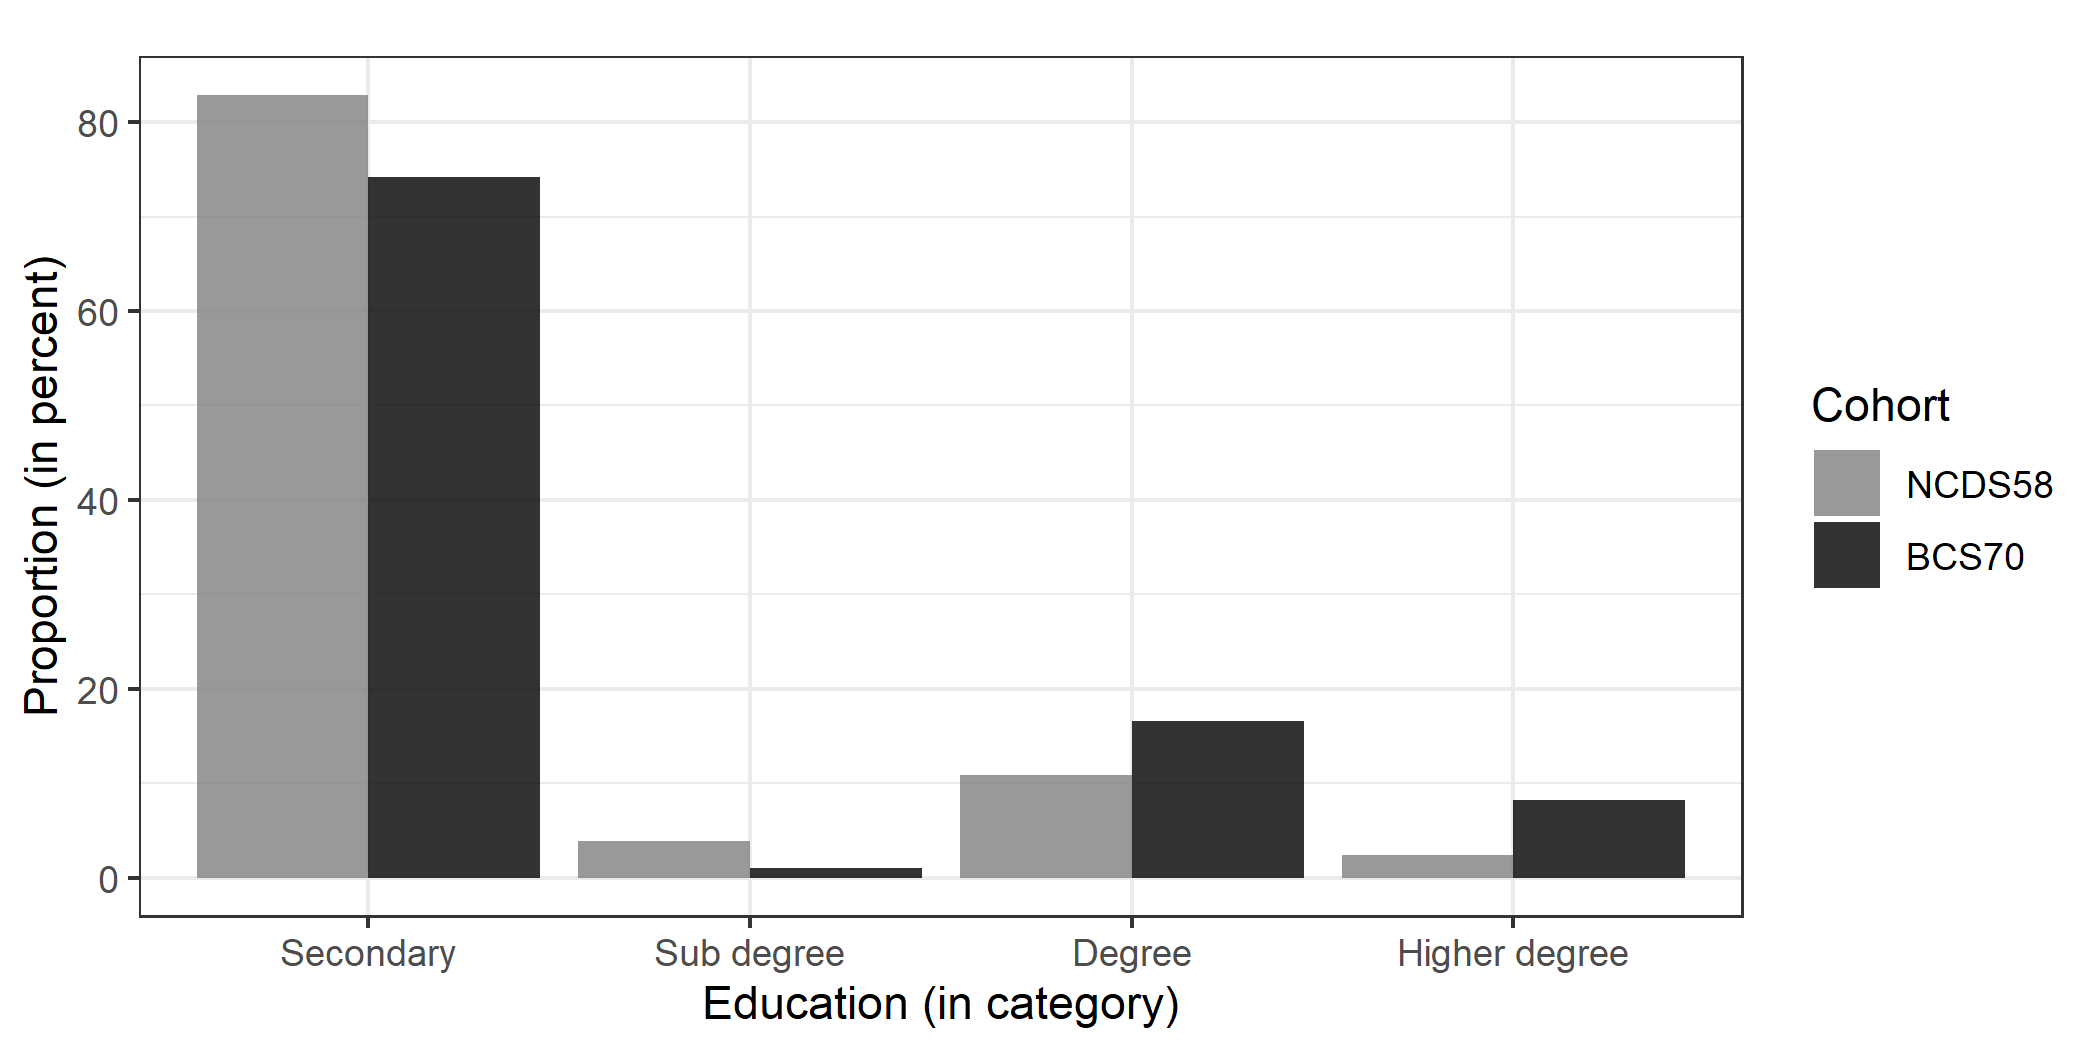
\includegraphics[width=\linewidth]{chap2/graphic/stat-educ-child-short.png}
	\vspace{-3em}
	\justify\singlespacing\footnotesize{\textit{Notes:} This figure presents the distribution of child education for the NCDS58 and BCS70 cohorts. Education corresponds to the highest academic qualification obtained by the child. Education levels are grouped into four categories for readability.}
\end{figure}

\begin{figure}[!htb]
    \centering
    \caption{Parental education distribution}
    \label{chap2-fig:stat-educ-parents}
    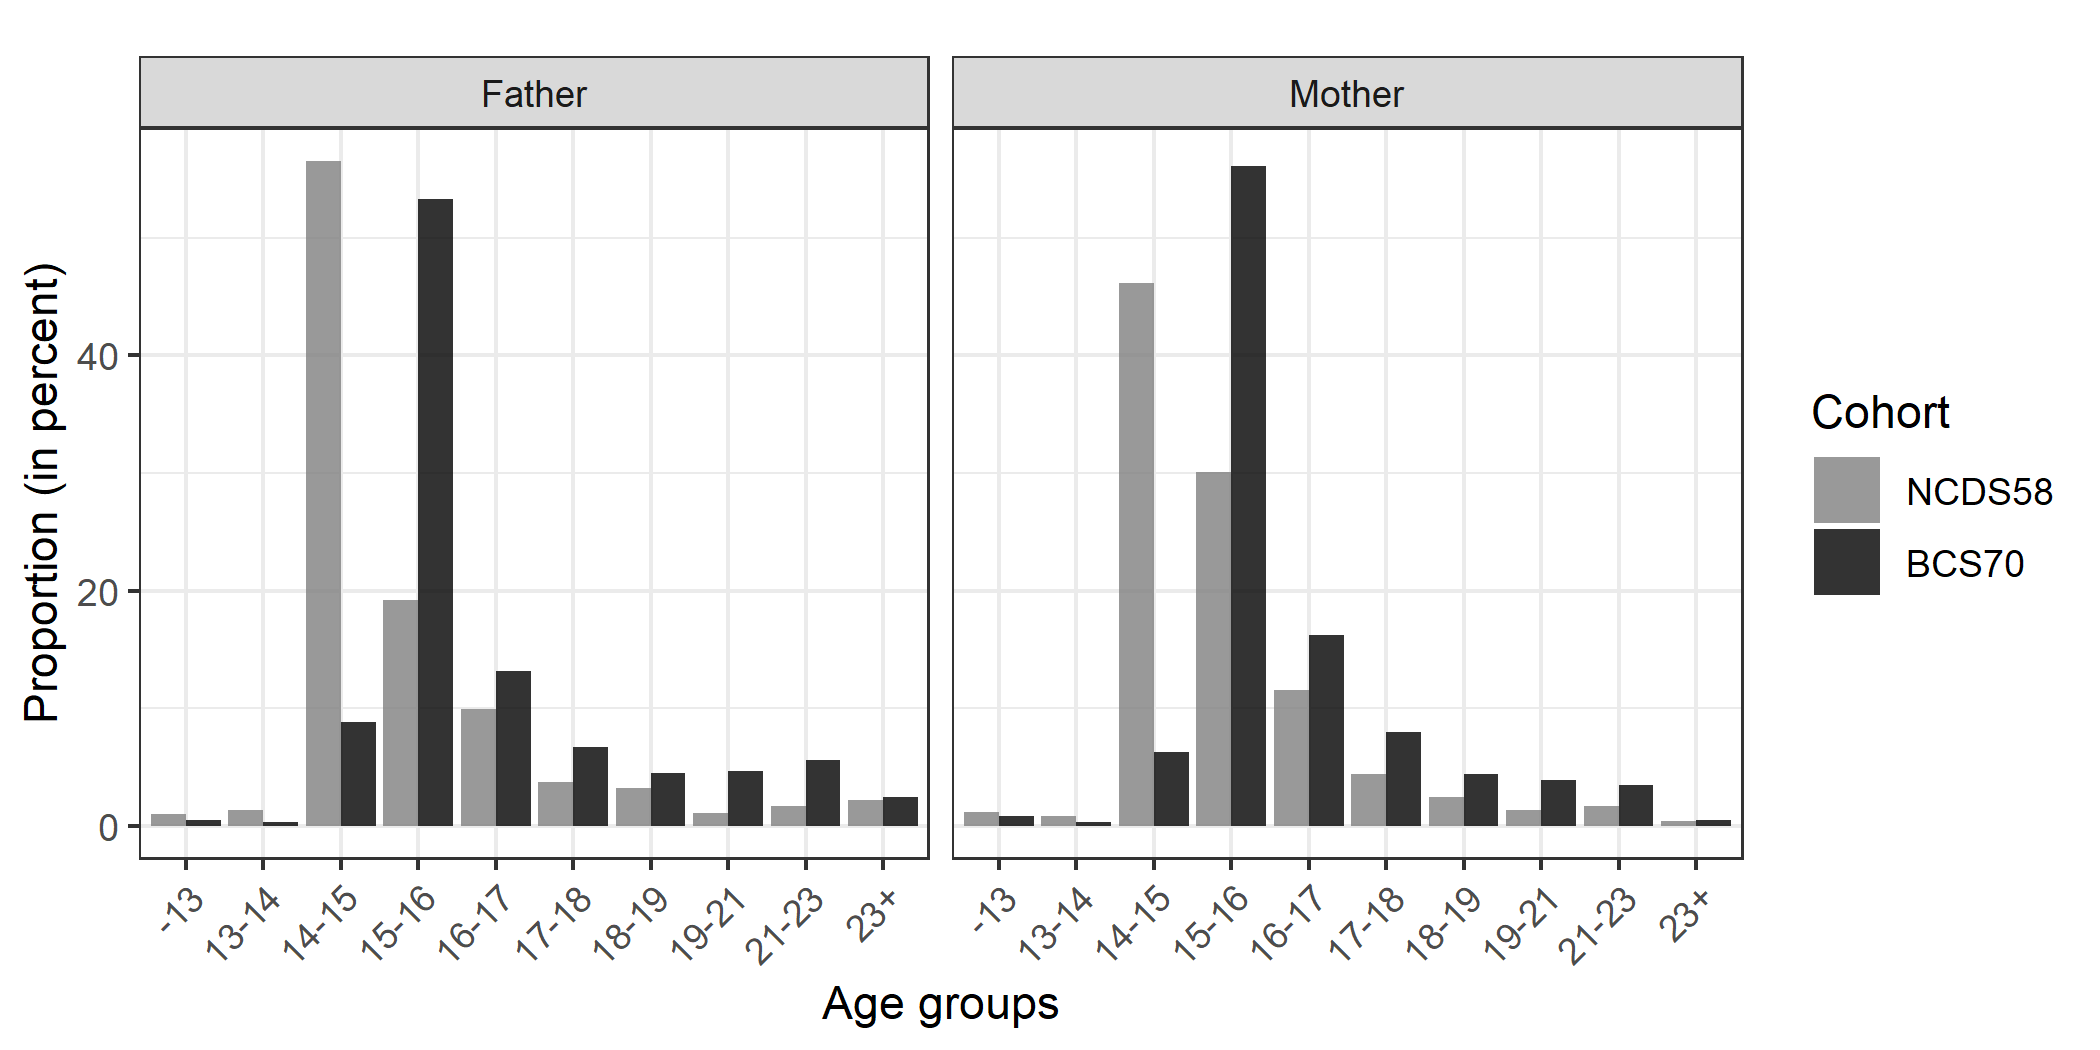
\includegraphics[width=\linewidth]{chap2/graphic/stat-educ-parents.png}
	\vspace{-3em}
	\justify\singlespacing\footnotesize{\textit{Notes:} This figure presents the distribution of parents' education for the NCDS58 and BCS70 cohorts. Parental education refers to the age at which parents left school that is used as a proxy. Education levels at the bottom and top are grouped for readability.}
\end{figure}

\textbf{Occupational structure.} In the data, occupations are reported according to e ISCO-88 categories. In Figure \ref{chap2-fig:stat-occ} we grouped occupations in three broad categories in line with the polarization literature, while Figure \ref{chap2-fig:polarize-isco88-both} performs a similar exercise using the original ISCO-88 categories. Occupations are depicted in light gray for those we place in the low-paying category, in dark grey for those in the middling category, and in black for high-paying ones. Although there are differences within the three broad categories, a clear pattern emerges both when we consider young and mature individuals. The change has been particularly large for young individual's occupations, for whom the reduction in the share of middling jobs has been marked. 

\begin{figure}[!htb]
     \centering
     \caption{Change in the probability of being in each ISCO-88 occupation in both periods}
     \label{chap2-fig:polarize-isco88-both}
     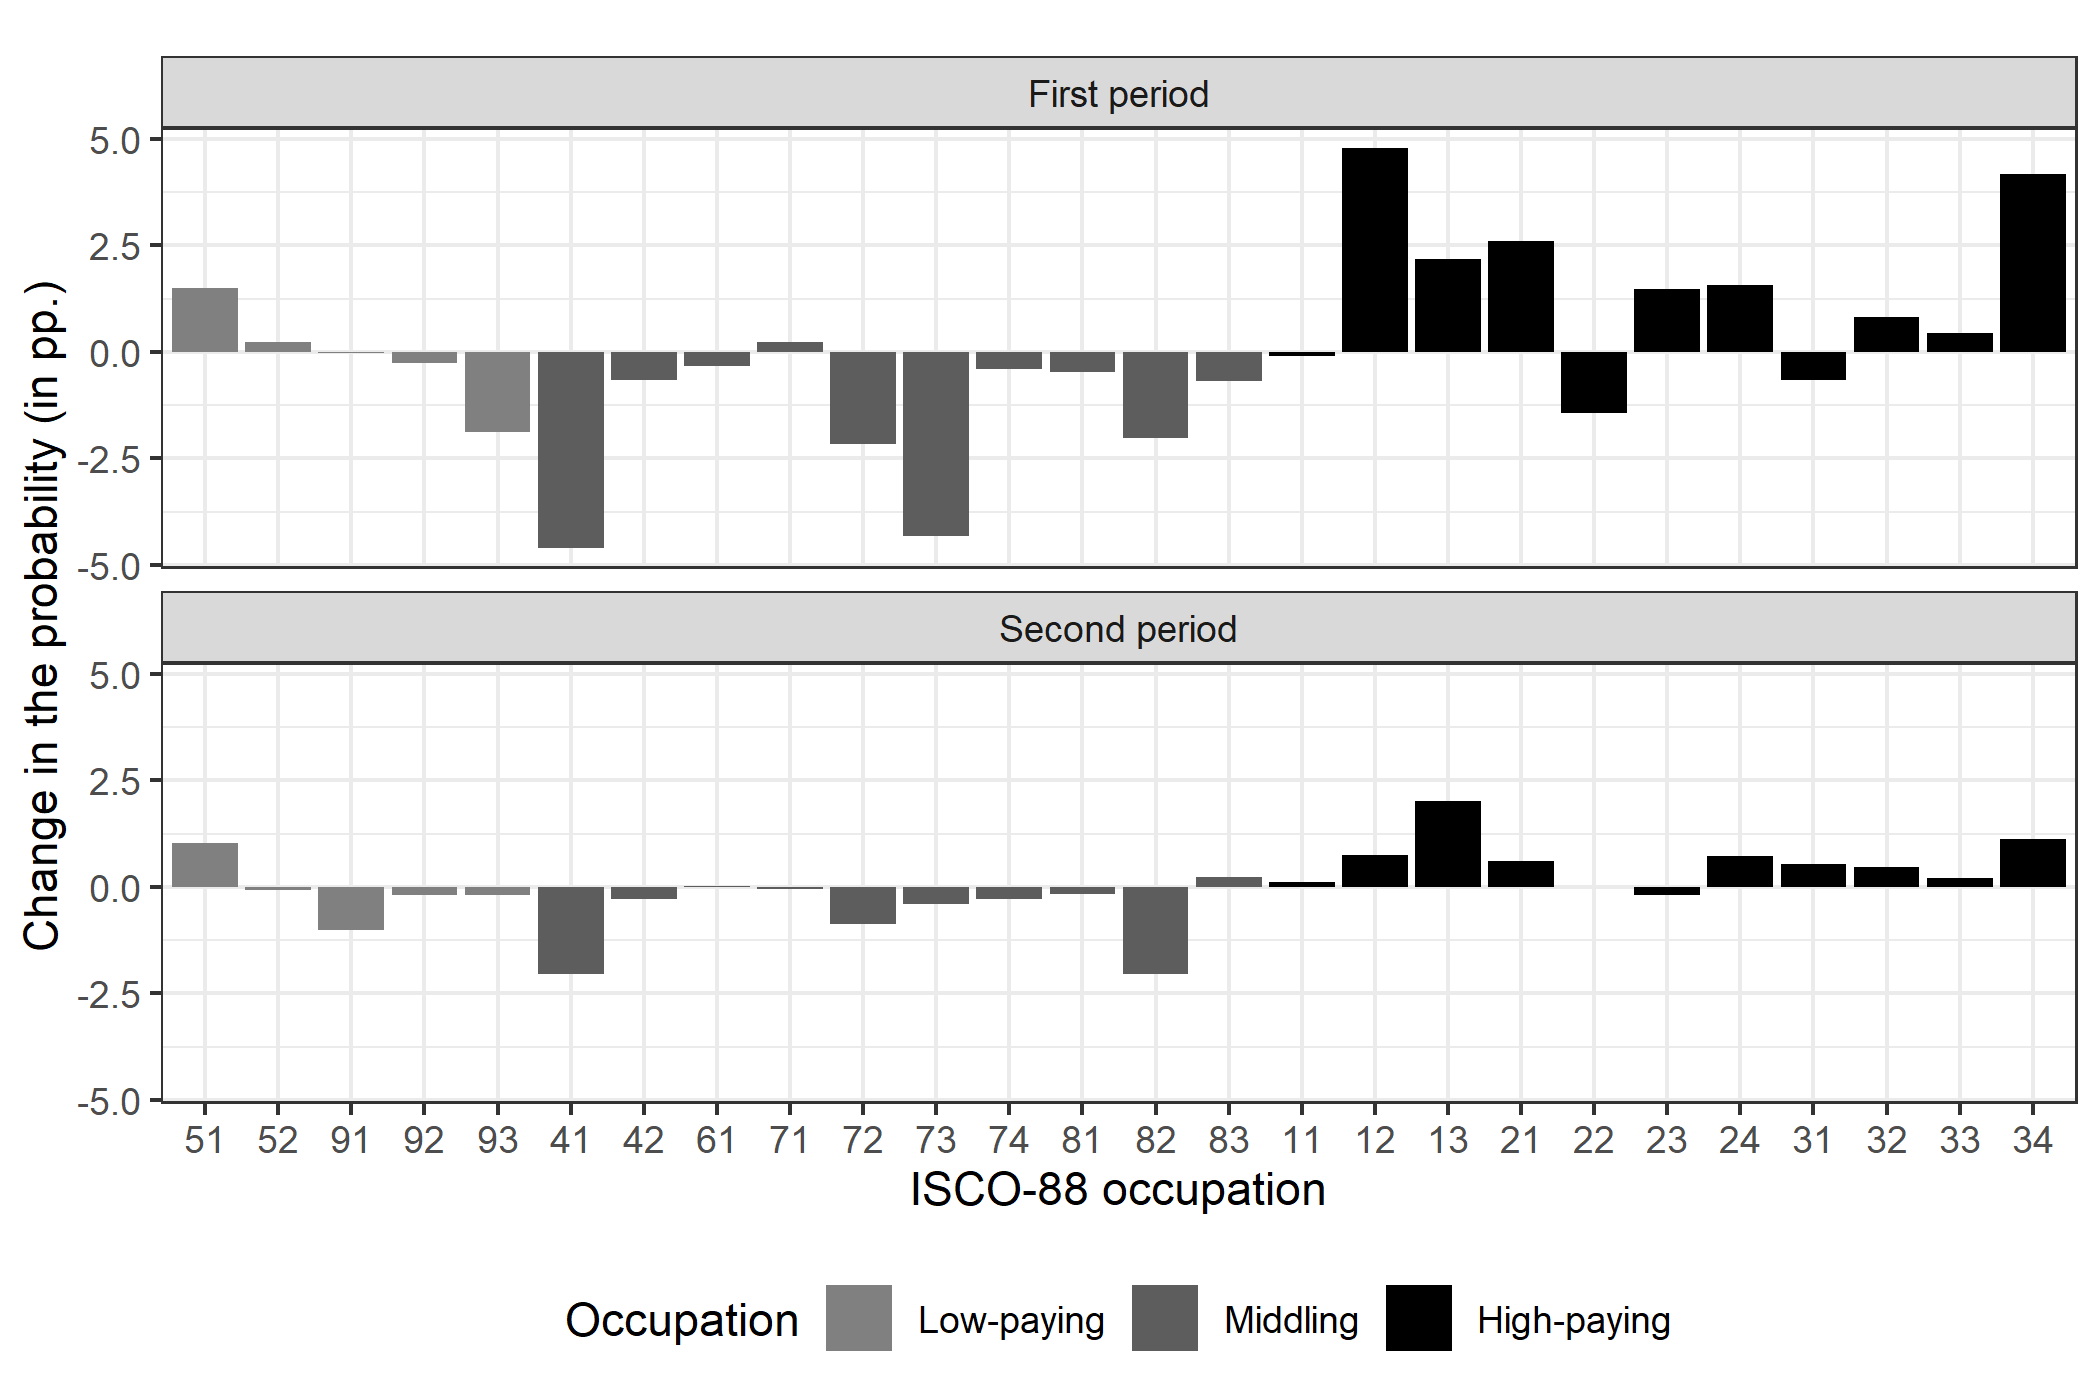
\includegraphics[width=\linewidth]{chap2/graphic/polarize-isco88-both.png}
 	\vspace{-3em}
 	\justify\singlespacing\footnotesize{\textit{Notes:} This figure presents the difference, expressed in percentage points, between the BCS70 and NCDS58 cohorts in terms of probability of being in each ISCO-88 occupation in both periods.}
\end{figure}


\subsubsection{The Labour Force Survey (1981-2012)}\label{chap2-app-data-LFS}

As a complementary dataset we use the Labor Force Survey (LFS). It is a random sampling of households living in the UK and collects data on labour market status and, since 1993, wages. The LFS was conducted every two years until 1983, then annually until 1992, and quarterly since then. It has the advantage of giving details on the occupation and industry in which individuals work, thus allowing us to take a snapshot of the structure of employment on a given year. The survey is intended to be representative of the whole population of the UK, and currently contains around 37,000 responding households in every quarter.

We use information from the LFS for the period 1981 to 2012, these being the years defined as the first-period for the older and the second-period for the younger cohorts. Initially the information is biannual, then annual from 1983 to 1992, and after that date we use data from the second quarter, as it is the one that most closely fits with the period over which annual interviews were conducted. The structure of the data allows us to define occupations in exactly the same way as for the cohort data and provides information on the region of employment.

Figure \ref{chap2-fig:lfs-national} shows the extent of job polarization at the national level using the LFS data. The share of middling jobs has declined by over 20 percentage points from 1981 to 2012. This reduction has been offset by an increase in the share of high-paying occupations by 16 percentage points over the same period, whereas the share of low-paying jobs has increased by 7 percentage points.
\begin{figure}[!htb]
    \centering
    \caption{Job polarization at the national level (The Labour Force Survey)}
    \label{chap2-fig:lfs-national}
    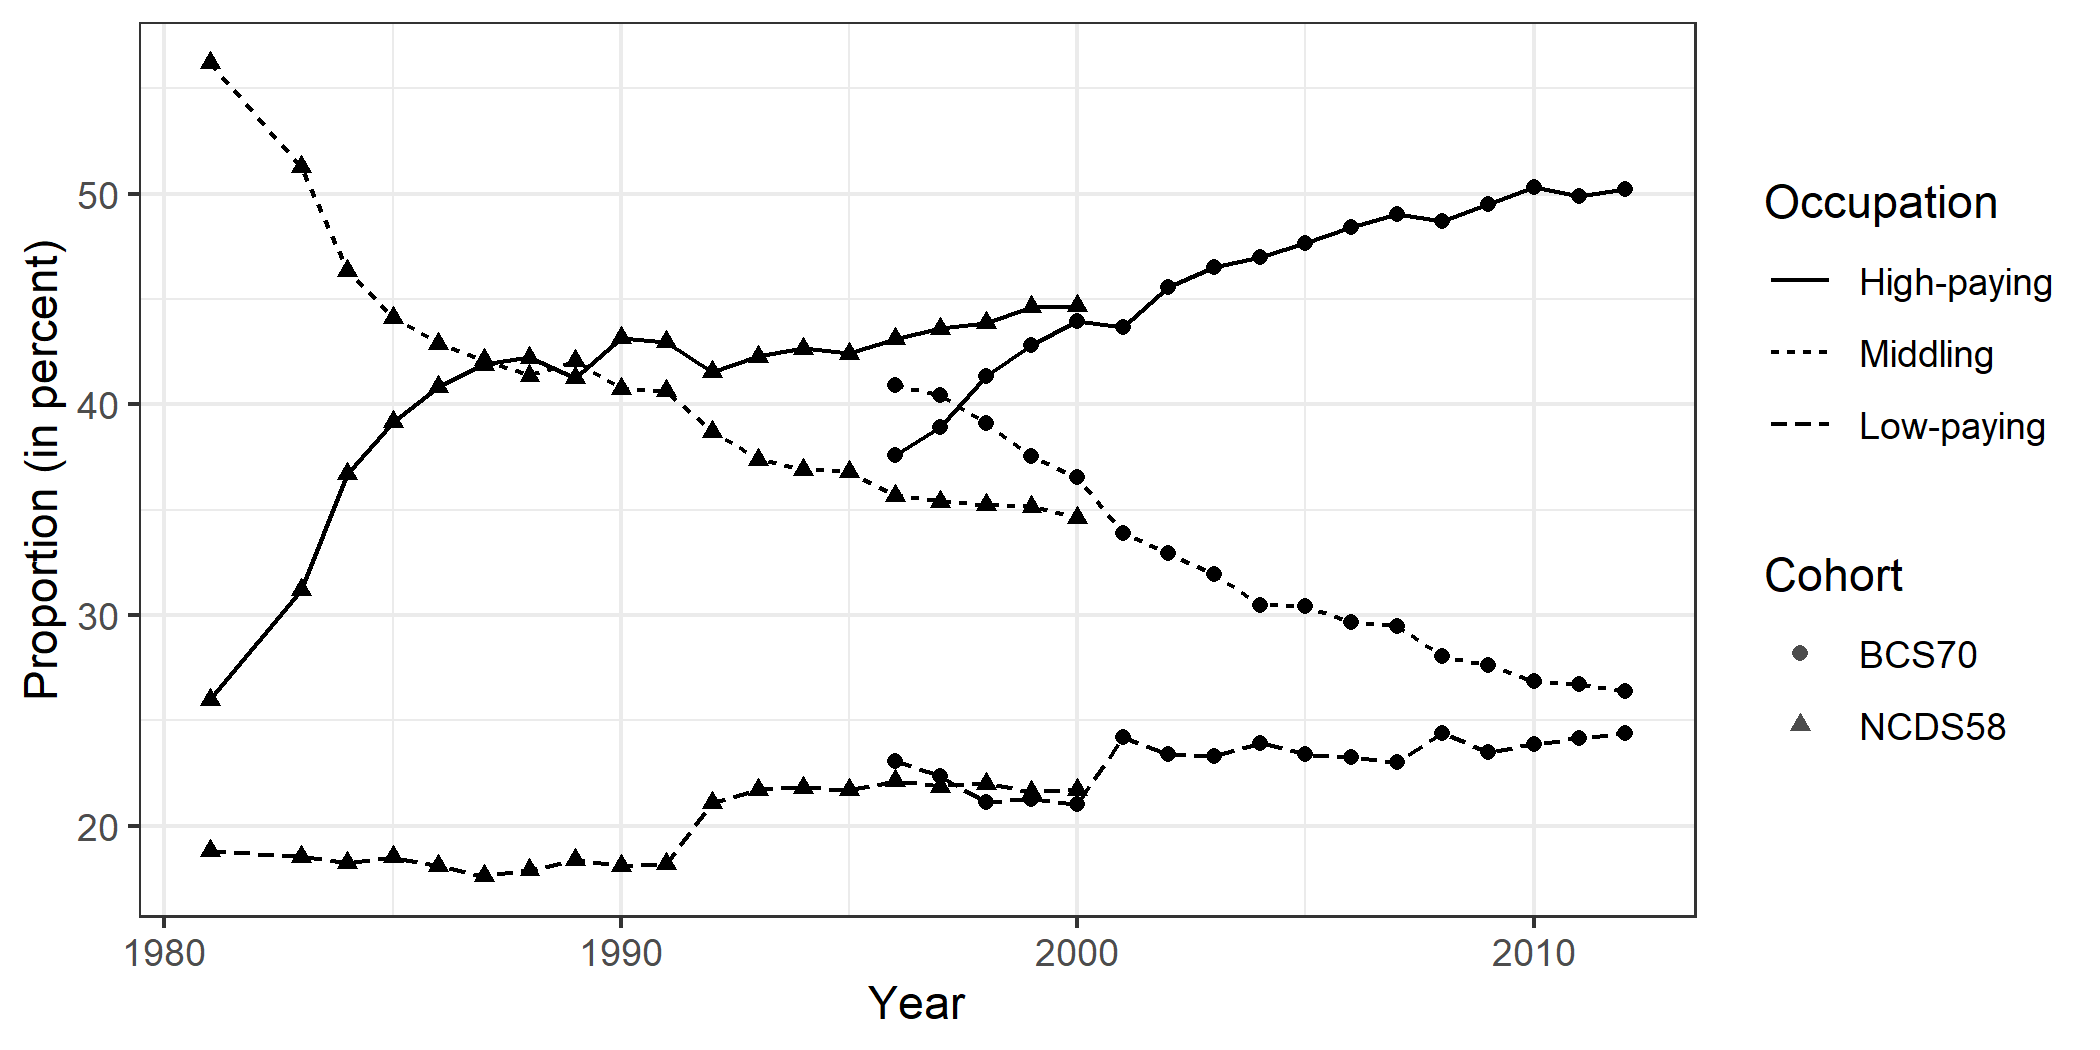
\includegraphics[width=\linewidth]{chap2/graphic/lfs-national.png}
	\vspace{-3em}
	\justify\singlespacing\footnotesize{\textit{Notes:} This figure presents the job polarization at the national level using the Labour Force Survey (LFS) data from 1981 to 2012. Curves represent the share of individuals in low-paying, middling, and high-paying occupations for the relevant age cohort in the LFS, i.e. from those born five years before to those born five years latter.}
\end{figure}

\begin{figure}[!htb]
    \centering
    \caption{Job polarization at the regional level over the lifecycle of both cohorts}
    \label{chap2-fig:lfs-regional}
    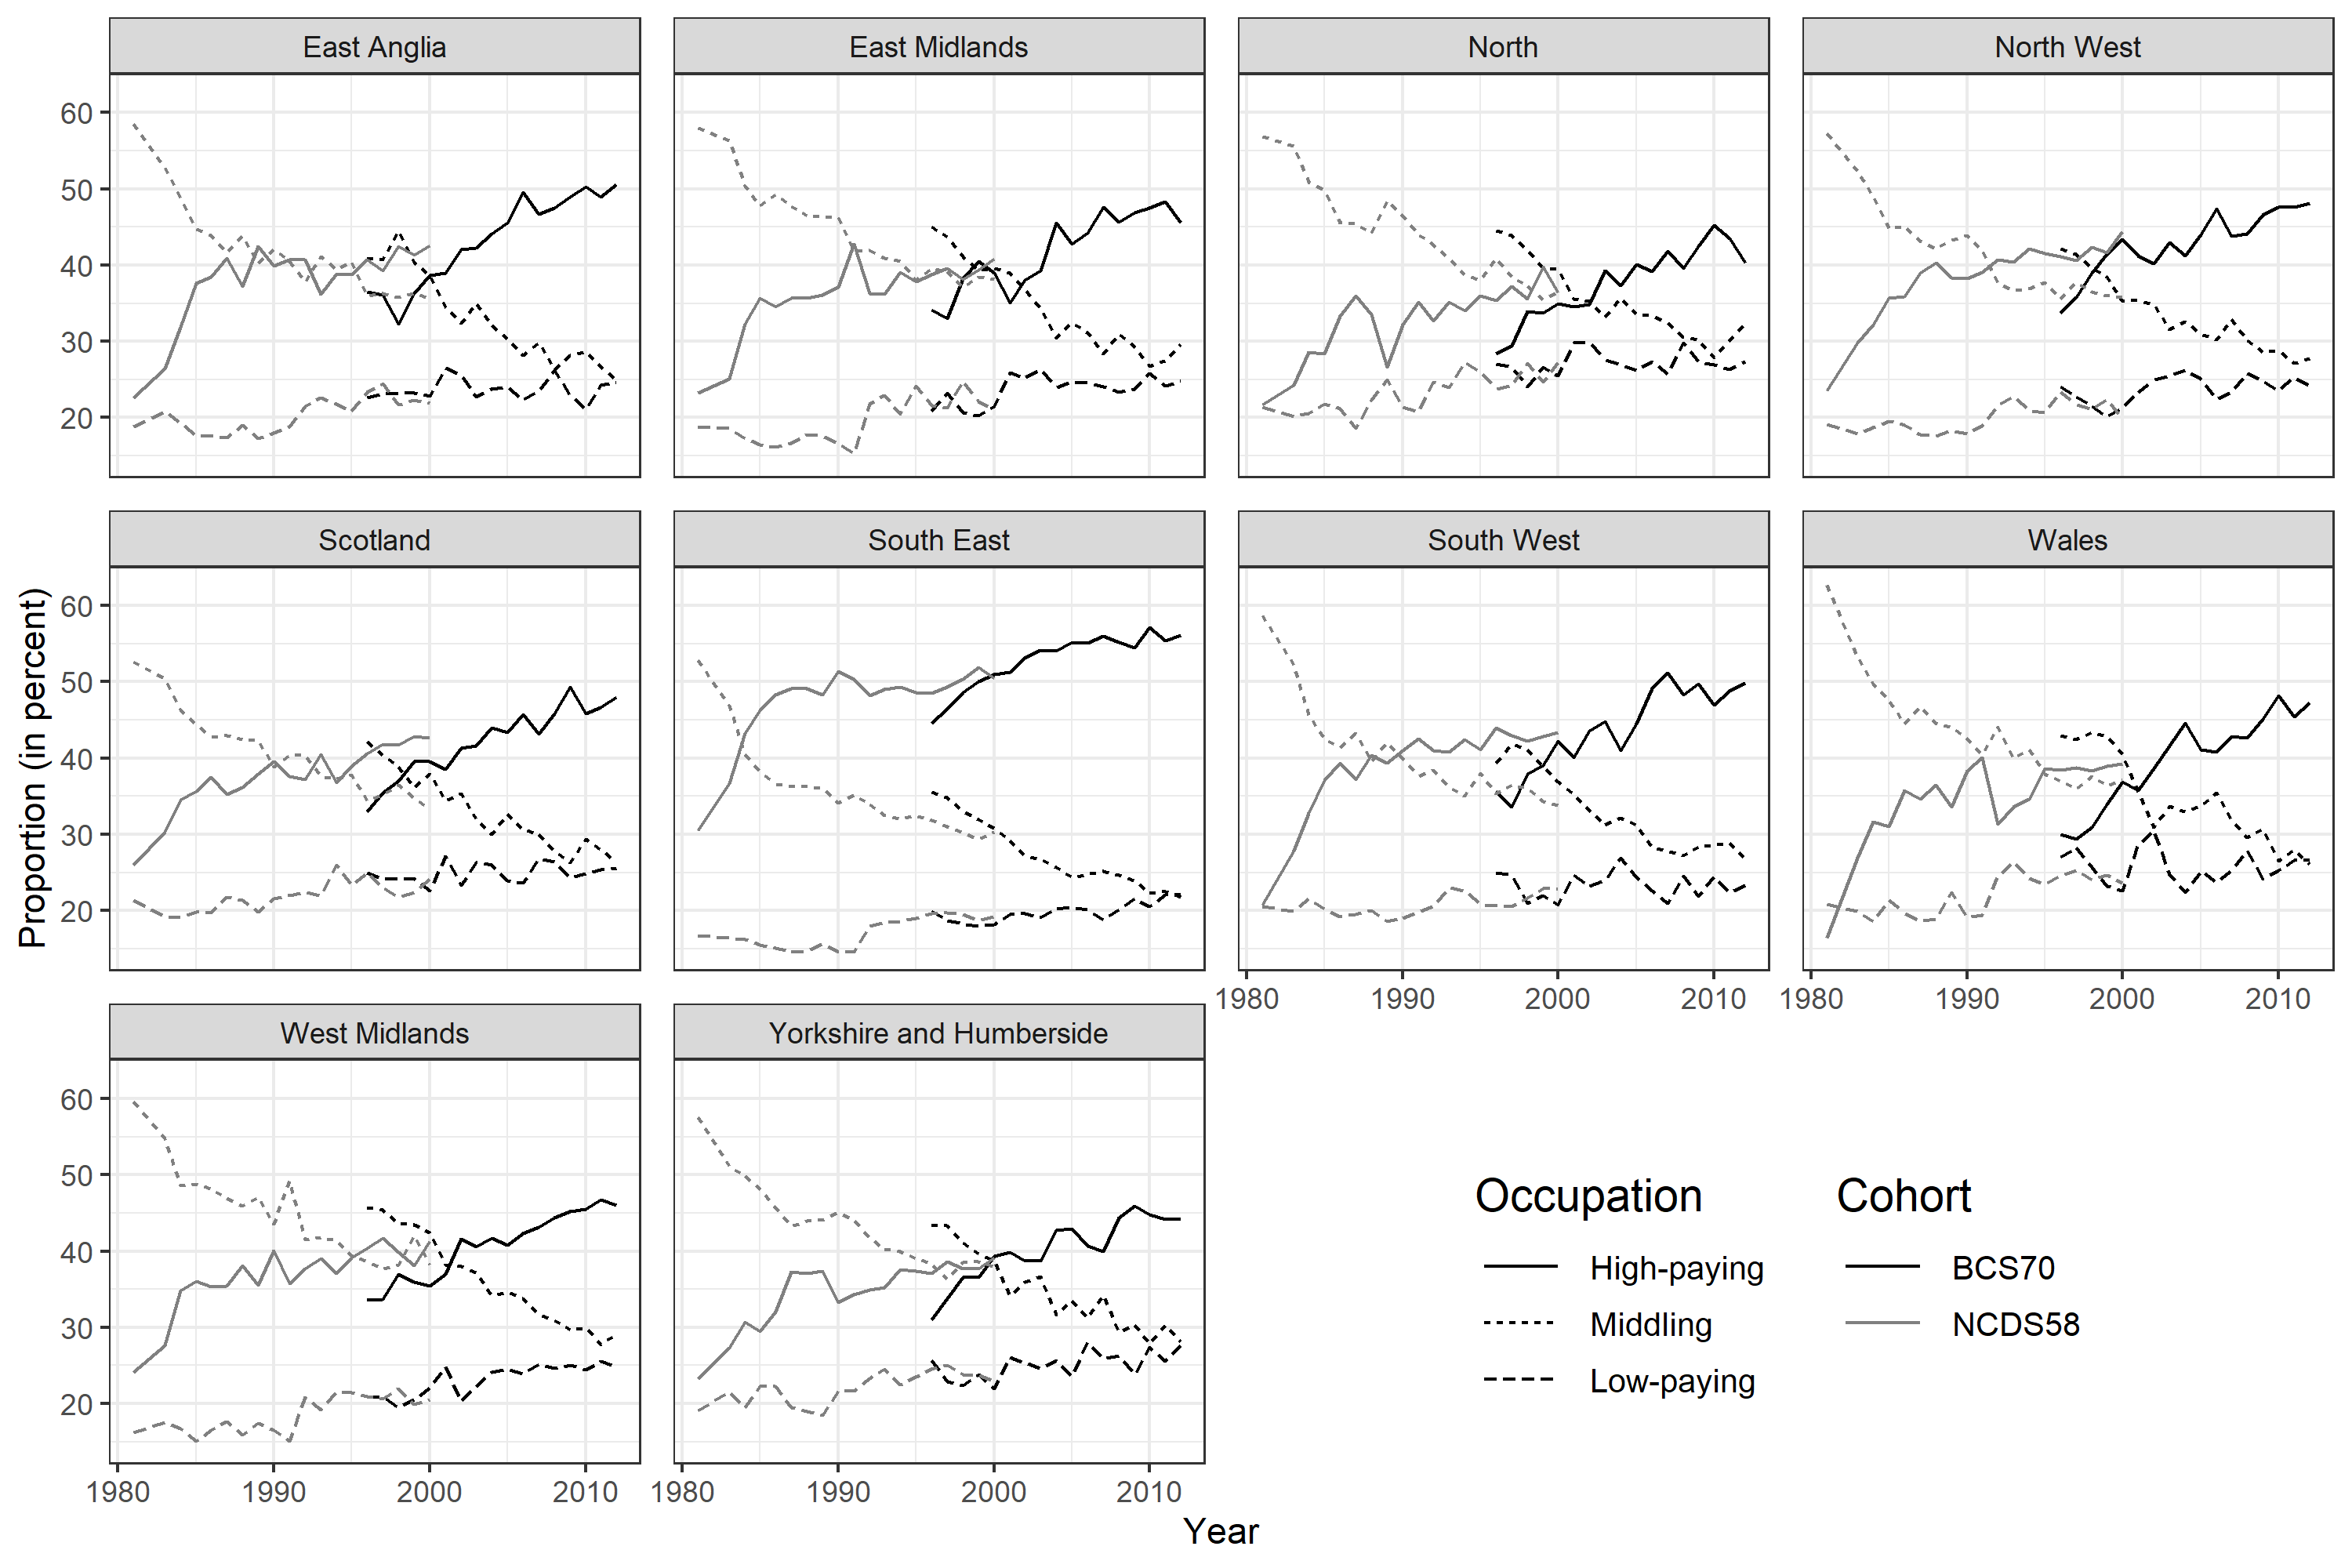
\includegraphics[width=\linewidth]{chap2/graphic/lfs-regional.png}
	\vspace{-3em}
	\justify\singlespacing\footnotesize{\textit{Notes:} This figure presents the job polarization at the regional level using the Labour Force Survey (LFS) data from 1981 to 2012. Curves represent the share of individuals in out-of-work, low-paying, middling, and high-paying occupations for the relevant age cohort in the LFS, i.e. from those born five years before to those born five years latter.}
\end{figure}

\subsubsection{Occupational classification}\label{chap2-app-data-classification}

Table \ref{chap2-tab:data-isco88} describes the classification of occupations that we use, providing an overview of ISCO-88 occupation codes along with the routine task intensities from \cite{Goos2014Explaining} and \cite{Mahutga2018Job}.
\begin{table}[!htb]
    \centering
    \begin{threeparttable}
        \caption{Overview of ISCO-88 occupation codes and routine task intensity}
        \label{chap2-tab:data-isco88}
        
\begin{tabular}{rlrr}
\toprule
\multicolumn{1}{c}{} & \multicolumn{1}{c}{} & \multicolumn{2}{c}{RTI} \\
\cmidrule(l{3pt}r{3pt}){3-4}
\textbf{Code} & \textbf{Occupation} & \textbf{GMS} & \textbf{LIS}\\
\midrule
\addlinespace[0.3em]
\multicolumn{4}{l}{\textbf{High-paying occupations}}\\
\hspace{1em}11 & Legislators and senior officials &  & -0.54\\
\hspace{1em}12 & Corporate managers & -0.75 & -0.62\\
\hspace{1em}13 & Managers of small enterprises & -1.52 & -1.41\\
\hspace{1em}21 & Physical, mathematical and engineering professionals & -0.82 & -0.70\\
\hspace{1em}22 & Life science and health professionals & -1.00 & -0.88\\
\hspace{1em}23 & Teaching professionals &  & -1.43\\
\hspace{1em}24 & Other professionals & -0.73 & -0.61\\
\hspace{1em}31 & Physical, mathematical and engineering associate professionals & -0.40 & -0.27\\
\hspace{1em}32 & Life science and health associate professionals & -0.33 & -0.20\\
\hspace{1em}33 & Teaching associate professionals &  & -1.33\\
\hspace{1em}34 & Other associate professionals & -0.44 & -0.32\\
\addlinespace[0.3em]
\multicolumn{4}{l}{\textbf{Middling occupations}}\\
\hspace{1em}41 & Office clerks & 2.24 & 2.39\\
\hspace{1em}42 & Customer service clerks & 1.41 & 1.55\\
\hspace{1em}61 & Skilled agricultural and fishery workers &  & 0.16\\
\hspace{1em}71 & Extraction and building trades workers & -0.19 & -0.06\\
\hspace{1em}72 & Metal, machinery and related trade work & 0.46 & 0.59\\
\hspace{1em}73 & Precision, handicraft, craft printing and related trade workers & 1.59 & 1.73\\
\hspace{1em}74 & Other craft and related trade workers & 1.24 & 1.38\\
\hspace{1em}81 & Stationary plant and related operators & 0.32 & 0.46\\
\hspace{1em}82 & Machine operators and assemblers & 0.49 & 0.63\\
\hspace{1em}83 & Drivers and mobile plant operators & -1.50 & -1.38\\
\addlinespace[0.3em]
\multicolumn{4}{l}{\textbf{Low-paying occupations}}\\
\hspace{1em}51 & Personal and protective service workers & -0.60 & -0.47\\
\hspace{1em}52 & Models, salespersons and demonstrators & 0.05 & 0.18\\
\hspace{1em}91 & Sales and service elementary occupations & 0.03 & 0.16\\
\hspace{1em}92 & Agricultural, fishery and related labourers &  & 0.39\\
\hspace{1em}93 & Laborers in mining, construction, manufacturing and transport & 0.45 & 0.58\\
\bottomrule
\end{tabular}

        \begin{tablenotes}[flushleft]
            \footnotesize{\item \textit{Notes}: This table provides an overview of ISCO-88 occupation codes and their corresponding Routine Task Intensity (RTI) from \cite{Goos2014Explaining} (GMS) and \cite{Mahutga2018Job} (LIS). Occupation groups (high-paying, middling and low-paying) correspond to those from \cite{Goos2014Explaining}, except for occupations 11, 23, 34, 61 and 92 that were removed from their analysis. We add these missing occupations to categories according to closest occupations, hence, relying on the 1-digit ISCO-88 classification.}
        \end{tablenotes}
    \end{threeparttable}
\end{table}
Table \ref{chap2-tab:stat-cohper} displays the shares of the various activity status and occupational categories.
\begin{table}[!htb]
    \centering
    \caption{Summary statistics - Cohort data per period}
    \label{chap2-tab:stat-cohper}
    \begin{threeparttable}
        % \setlength{\tabcolsep}{3pt}
        
\begin{tabular}{lrrrrrrrr}
\toprule
\multicolumn{1}{c}{} & \multicolumn{4}{c}{NCDS58 - N = 6780} & \multicolumn{4}{c}{BCS70 - N = 7992} \\
\cmidrule(l{3pt}r{3pt}){2-5} \cmidrule(l{3pt}r{3pt}){6-9}
\multicolumn{1}{c}{} & \multicolumn{2}{c}{First period} & \multicolumn{2}{c}{Second period} & \multicolumn{2}{c}{First period} & \multicolumn{2}{c}{Second period} \\
\cmidrule(l{3pt}r{3pt}){2-3} \cmidrule(l{3pt}r{3pt}){4-5} \cmidrule(l{3pt}r{3pt}){6-7} \cmidrule(l{3pt}r{3pt}){8-9}
Variable & Mean & SD & Mean & SD & Mean & SD & Mean & SD\\
\midrule
Activity - Employee & 0.74 & 0.44 & 0.74 & 0.44 & 0.78 & 0.42 & 0.72 & 0.45\\
Activity - Self-employed & 0.05 & 0.21 & 0.12 & 0.33 & 0.06 & 0.24 & 0.14 & 0.35\\
Activity - Unemployed & 0.05 & 0.23 & 0.02 & 0.14 & 0.02 & 0.16 & 0.02 & 0.14\\
Activity - in Education & 0.02 & 0.15 & 0.01 & 0.08 & 0.03 & 0.16 & 0.00 & 0.06\\
Activity - Inactive & 0.14 & 0.34 & 0.12 & 0.32 & 0.11 & 0.31 & 0.11 & 0.32\\
Occupation - High-paying & 0.24 & 0.42 & 0.39 & 0.49 & 0.36 & 0.48 & 0.44 & 0.50\\
Occupation - Middling & 0.41 & 0.49 & 0.28 & 0.45 & 0.33 & 0.47 & 0.24 & 0.43\\
Occupation - Low-paying & 0.14 & 0.35 & 0.19 & 0.39 & 0.15 & 0.36 & 0.18 & 0.39\\
Occupation - Out-of-work & 0.19 & 0.39 & 0.14 & 0.34 & 0.13 & 0.34 & 0.14 & 0.34\\
Occupation - in Education & 0.02 & 0.15 & 0.01 & 0.08 & 0.03 & 0.16 & 0.00 & 0.06\\
Pay & 19.06 & 7.23 & 30.35 & 24.20 & 25.21 & 16.47 & 36.01 & 25.54\\
\bottomrule
\end{tabular}

        \begin{tablenotes}[flushleft]
            \footnotesize{\item \textit{Notes}: This table provides summary statistics for individual time-variant data from the BCS70 and NCDS58 according to the period.}
        \end{tablenotes}
    \end{threeparttable}
\end{table}
Table \ref{chap2-tab:stat-pay} reports the average weekly pay by occupation in the cohort data. Weekly pay is more concentrated for young individuals than for mature ones, as wages tend to grow faster with age for those in high-paying occupations. The table indicates that the average pay has increased for every type of occupation between both cohorts. The change across cohort of pay at age 42 is roughly the same for the three categories, lying between 14 and 15\%. In contrast, for young individuals, the change has been much larger for those in high-paying occupations (50\%) than for the other two groups (13 and 20\%, respectively, in low-paying and middling occupations).

\begin{table}[!htb]
    \centering
    \caption{Average weekly pay by occupation (in 1970£)}
    \label{chap2-tab:stat-pay}
    \begin{threeparttable}
        \setlength{\tabcolsep}{18pt}
        \begin{tabular}{l D{.}{.}{3.3} D{.}{.}{3.3} D{.}{.}{3.3} D{.}{.}{3.3}}
\toprule
\multicolumn{1}{c}{} & \multicolumn{2}{c}{First period} & \multicolumn{2}{c}{Second period} \\
\cmidrule(l{3pt}r{3pt}){2-3} \cmidrule(l{3pt}r{3pt}){4-5}
Occupation & \multicolumn{1}{c}{NCDS58} & \multicolumn{1}{c}{BCS70} & \multicolumn{1}{c}{NCDS58} & \multicolumn{1}{c}{BCS70}\\
\midrule
Low-paying & 17.05 & 19.35 & 17.75 & 20.25\\
 & (0.30) & (0.61) & (0.39) & (0.37)\\
Middling & 19.60 & 23.42 & 25.26 & 29.07\\
 & (0.16) & (0.34) & (0.45) & (0.39)\\
High-paying & 19.51 & 29.23 & 40.82 & 46.64\\
 & (0.17) & (0.40) & (0.64) & (0.55)\\
\bottomrule
\end{tabular}

        \begin{tablenotes}[flushleft]
            \footnotesize{\item \textit{Notes}: This table presents the average weekly pay, expressed in 1970£, in each first- and second-period occupations for the NCDS58 and BCS70 cohorts. Standard errors between parentheses. We exclude the very bottom and top of the pay distribution for each cohort, i.e. pay which are below £1 and above £300.}
        \end{tablenotes}
    \end{threeparttable}
\end{table}

Occupations are also characterized by different educational requirements. Note, however, that a comparison across the two cohorts is not straight forward as the overall educational attainment of the population has increased, as seen in Figure \ref{chap2-fig:stat-educ-child-short}. Because of these changes, Table \ref{chap2-tab:stat-educ} reports average education by occupation using the peer-inclusive downward-looking ranking. As well as our three employment categories we also report the educational attainment of those who are not in employment, splitting this category into those in full time education and the rest of those who are out-of-work (unemployed or not participating).\footnote{In our data, child education is time invariant because we consider the highest qualification ever obtained. Although some individuals may still appear in the occupational category full-time education, their educational level is the one they will obtain in the future.} When we do not split this category we find that average education is rather high, this being the combination of the low attainment of those not participating or unemployed and the high attainment of those still in education.

\begin{table}[!htb]
    \centering
    \caption{Average education by occupations}
    \label{chap2-tab:stat-educ}
    \begin{threeparttable}
        \setlength{\tabcolsep}{18pt}
        \begin{tabular}{l D{.}{.}{3.3} D{.}{.}{3.3} D{.}{.}{3.3} D{.}{.}{3.3}}
\toprule
\multicolumn{1}{c}{} & \multicolumn{2}{c}{First period} & \multicolumn{2}{c}{Second period} \\
\cmidrule(l{3pt}r{3pt}){2-3} \cmidrule(l{3pt}r{3pt}){4-5}
Occupation & \multicolumn{1}{c}{NCDS58} & \multicolumn{1}{c}{BCS70} & \multicolumn{1}{c}{NCDS58} & \multicolumn{1}{c}{BCS70}\\
\midrule
Out-of-work & 0.55 & 0.51 & 0.54 & 0.54\\
 & (0.01) & (0.01) & (0.01) & (0.01)\\
Education & 0.89 & 0.79 & 0.84 & 0.62\\
 & (0.01) & (0.01) & (0.03) & (0.05)\\
Low-paying & 0.54 & 0.52 & 0.52 & 0.51\\
 & (0.01) & (0.01) & (0.00) & (0.00)\\
Middling & 0.58 & 0.54 & 0.55 & 0.53\\
 & (0.00) & (0.00) & (0.00) & (0.00)\\
High-paying & 0.74 & 0.72 & 0.73 & 0.70\\
 & (0.01) & (0.00) & (0.00) & (0.00)\\
\bottomrule
\end{tabular}

        \begin{tablenotes}[flushleft]
            \footnotesize{\item \textit{Notes}: This table presents the average education, expressed in peer-inclusive downward-looking ranking, in each first- and second-period occupations for the NCDS58 and BCS70 cohorts. Standard errors between parentheses.}
        \end{tablenotes}
    \end{threeparttable}
\end{table}

\subsubsection{Structure of employment}\label{chap2-app-data-structure}

Table \ref{chap2-tab:proba-group4-abs} presents the probability to be in each occupation at both periods, for both cohorts. The first-period probabilities indicate that BCS70-cohort individuals are about 7.9 pp. less likely to start in middling occupations, while they are about 12.4 pp. more likely to start their careers in a high-paying occupation. The probabilities with those in education in a separate category, hence not included in out-of-work, are reported in Table \ref{chap2-tab:proba-group5-abs}. Table \ref{chap2-tab:proba-group5-cdt-short} provides the probability of being in each second-period occupation conditional on the first-period occupation, isolating those in-education from the out-of-work. 

\begin{table}[!htb]
    \centering
    \caption{Probability of being in each occupation at both periods, for both cohorts (in percent)}
    \label{chap2-tab:proba-group4-abs}
    \begin{threeparttable}
        \setlength{\tabcolsep}{10pt}
        
\begin{tabular}{lrrrrrr}
\toprule
\multicolumn{1}{c}{} & \multicolumn{3}{c}{First period} & \multicolumn{3}{c}{Second period} \\
\cmidrule(l{3pt}r{3pt}){2-4} \cmidrule(l{3pt}r{3pt}){5-7}
Occupation & BCS70 & NCDS58 & $\Delta$ & BCS70 & NCDS58 & $\Delta$\\
\midrule
Out-of-work & 16.2 & 21.3 & -5.1 & 13.9 & 14.4 & -0.4\\
Low-paying & 15.2 & 14.0 & 1.2 & 18.4 & 19.1 & -0.7\\
Middling & 33.1 & 41.2 & -8.1 & 23.8 & 28.0 & -4.2\\
High-paying & 35.6 & 23.6 & 12.1 & 43.9 & 38.5 & 5.4\\
\bottomrule
\end{tabular}

        \begin{tablenotes}[flushleft]
            \footnotesize{\item \textit{Notes}: This table shows the probability, expressed in percent, of being in each first- and second-period occupation for the BCS70 and NCDS58 cohorts. Differences between both cohorts, expressed in percentage points, are reported in the last column of both periods.}
        \end{tablenotes}
    \end{threeparttable}
\end{table}

\begin{table}[!htb]
     \centering
     \caption{Probability to be in each occupation at both periods, isolating those in-education (in percent)}
     \label{chap2-tab:proba-group5-abs}
    \begin{threeparttable}
        % \small
        \setlength{\tabcolsep}{10pt}
        
\begin{tabular}{lrrrrrr}
\toprule
\multicolumn{1}{c}{} & \multicolumn{3}{c}{First period} & \multicolumn{3}{c}{Second period} \\
\cmidrule(l{3pt}r{3pt}){2-4} \cmidrule(l{3pt}r{3pt}){5-7}
Occupation & BCS70 & NCDS58 & $\Delta$ & BCS70 & NCDS58 & $\Delta$\\
\midrule
Out-of-work & 13.5 & 19.1 & -5.6 & 13.6 & 13.7 & -0.1\\
in-Education & 2.7 & 2.2 & 0.5 & 0.3 & 0.6 & -0.3\\
Low-paying & 15.2 & 14.0 & 1.2 & 18.4 & 19.1 & -0.7\\
Middling & 33.1 & 41.2 & -8.1 & 23.8 & 28.0 & -4.2\\
High-paying & 35.6 & 23.6 & 12.1 & 43.9 & 38.5 & 5.4\\
\bottomrule
\end{tabular}

        \begin{tablenotes}[flushleft]
            \footnotesize{\item \textit{Notes}: This table shows the probability, expressed in percent, of being in each first- and second-period occupation for the BCS70 and NCDS58 cohorts. Differences between both cohorts, expressed in percentage points, are reported in the last column of both periods.}
        \end{tablenotes}
    \end{threeparttable}
\end{table}

\begin{table}[!htb]
    \centering
    \caption{Conditional probabilities of changing occupations during the career, isolating those in-education (in percent)}
    \label{chap2-tab:proba-group5-cdt-short}
    \resizebox{\textwidth}{!}{
    \begin{threeparttable}
        
\begin{tabular}{lrrrrrrrrrr}
\toprule
\multicolumn{1}{c}{} & \multicolumn{5}{c}{BCS70} & \multicolumn{5}{c}{NCDS58} \\
\cmidrule(l{3pt}r{3pt}){2-6} \cmidrule(l{3pt}r{3pt}){7-11}
Occupation & Out & Educ & Low & Mid & High & Out & Educ & Low & Mid & High\\
\midrule
Out-of-work & 37.0 & 0.7 & 28.3 & 15.2 & 18.9 & 28.5 & 0.9 & 26.9 & 22.1 & 21.6\\
in-Education & 14.0 & 0.5 & 10.7 & 11.2 & 63.7 & 10.7 & 0.0 & 5.3 & 8.0 & 76.0\\
Low-paying & 13.3 & 0.3 & 45.1 & 17.5 & 23.8 & 15.8 & 0.5 & 40.0 & 20.3 & 23.4\\
Middling & 10.2 & 0.3 & 13.8 & 44.9 & 30.8 & 9.9 & 0.5 & 15.4 & 43.4 & 30.8\\
High-paying & 8.0 & 0.2 & 8.2 & 11.0 & 72.6 & 7.6 & 0.8 & 8.1 & 12.3 & 71.2\\
\bottomrule
\end{tabular}

        \begin{tablenotes}[flushleft]
            \footnotesize{\item \textit{Notes}: Conditional probabilities with people in education included in out-of-work are reported in the paper, see table \ref{chap2-tab:proba-group4-cdt}.}
        \end{tablenotes}
    \end{threeparttable}
    }
\end{table}

Figure \ref{chap2-fig:polarize-isco88-pay-p3} presents the change in the frequencies of second period occupation according to the average weekly pay for the BCS70 cohort. 
Figure \ref{chap2-fig:polarize-rtiLIS-p3} displays the negative relationship between the probability of being in each second-period occupation according to its routine task intensity.

\begin{figure}[!htb]
    \centering
    \caption{Change in the probability of being in an occupation in the second period and average weekly pay}
    \label{chap2-fig:polarize-isco88-pay-p3}
    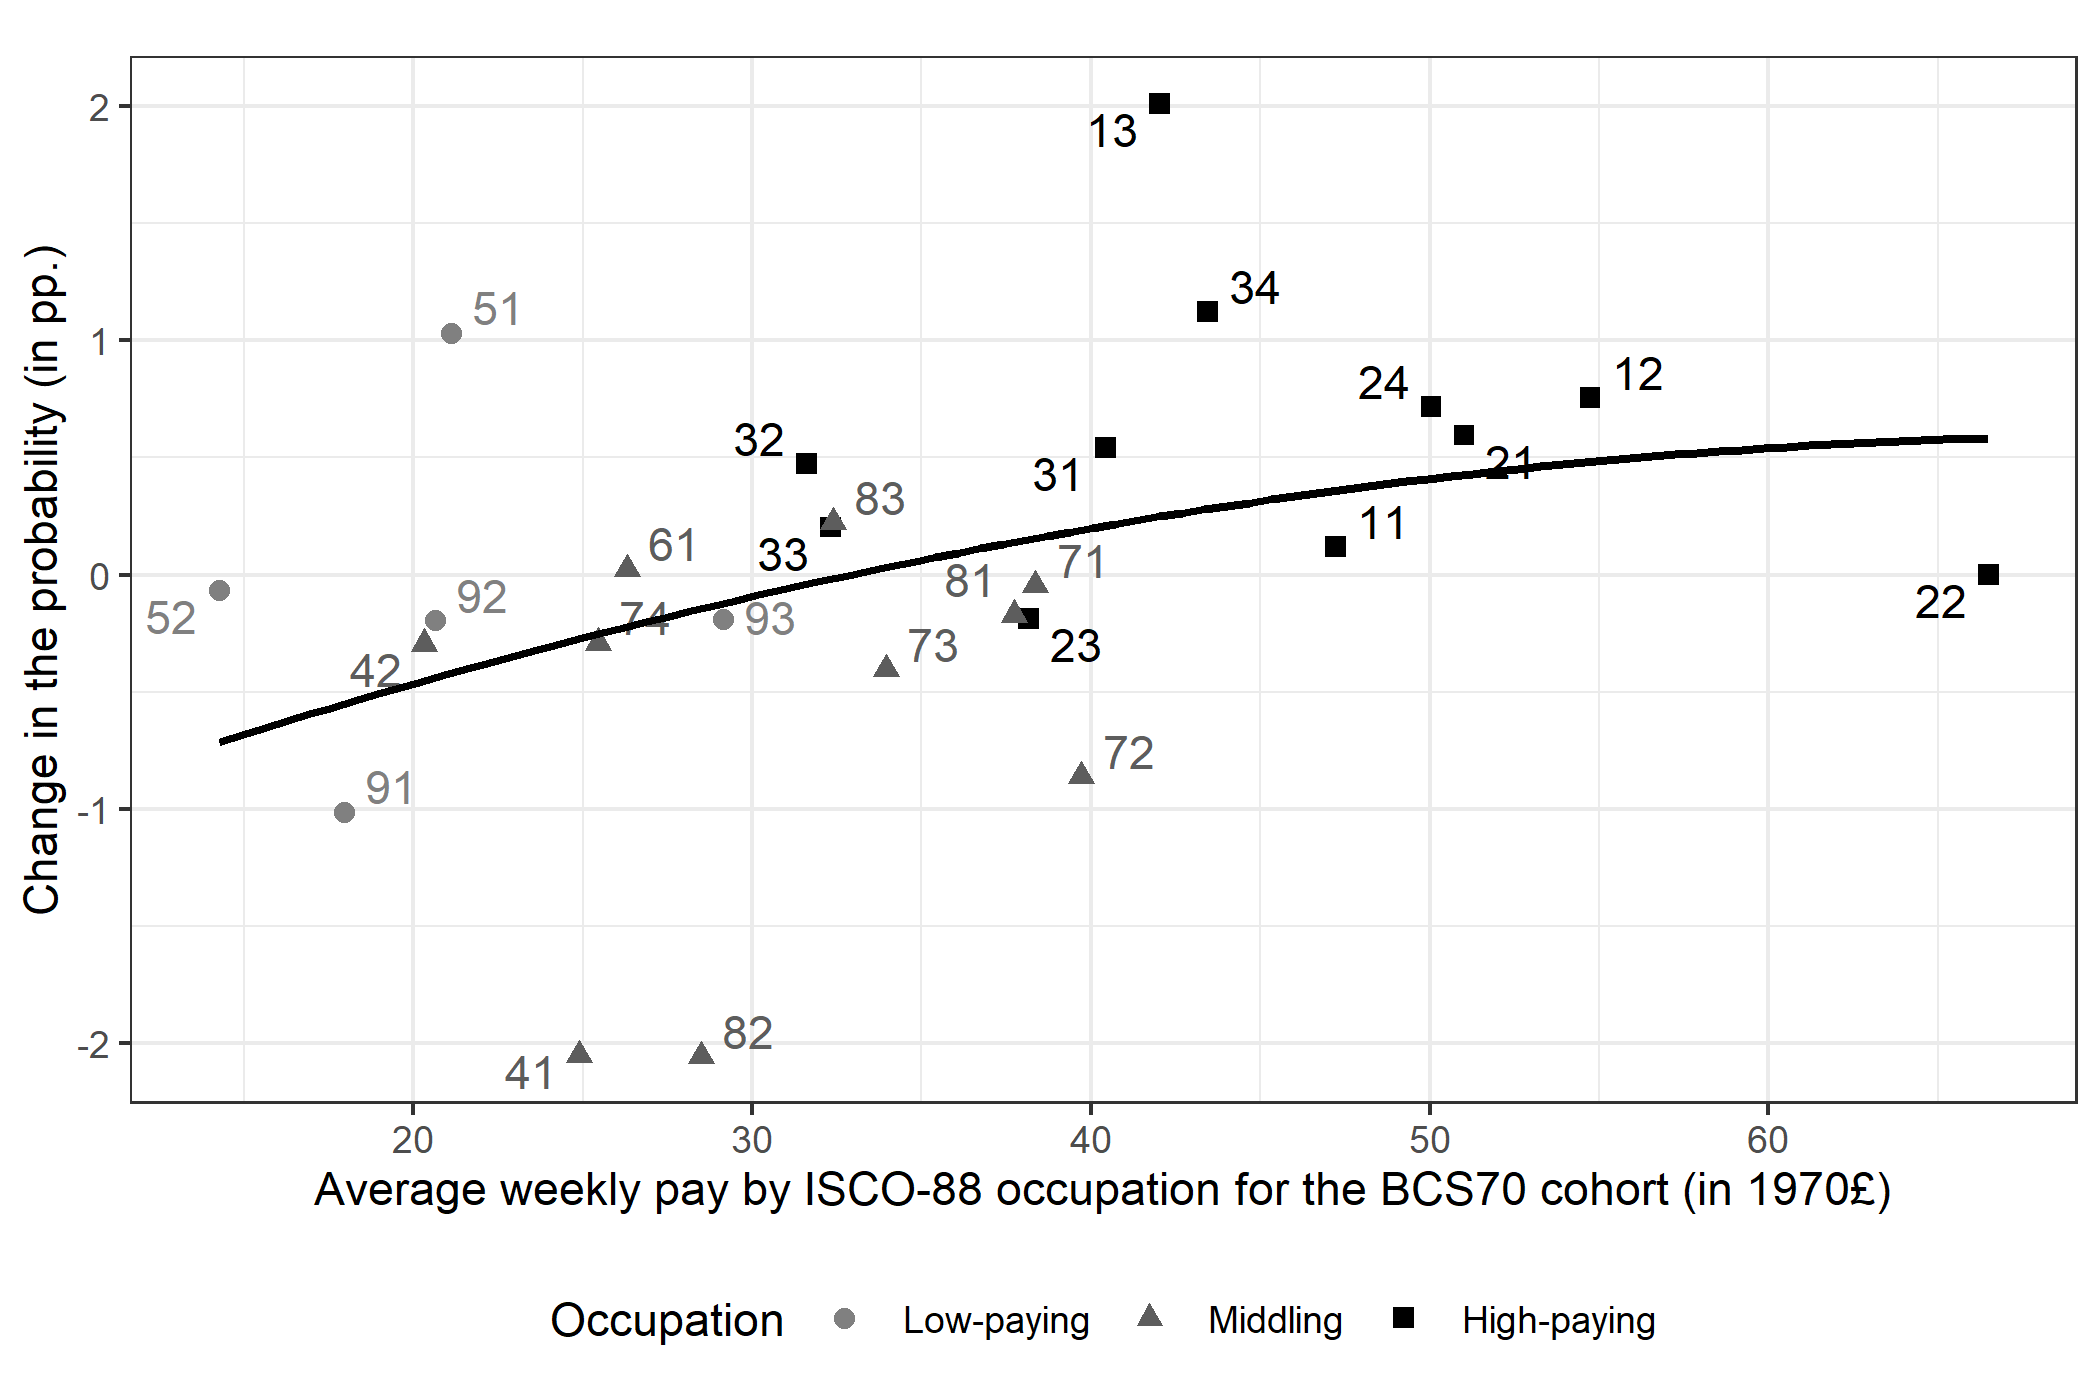
\includegraphics[width=\linewidth]{chap2/graphic/polarize-BCSpay-p3.png}
	\vspace{-3em}
	\justify\singlespacing\footnotesize{\textit{Notes:} This figure presents the positive relationship between the difference, expressed in percentage points, between the BCS70 and NCDS58 cohorts in terms of probability of being in each ISCO-88 occupation in second period and the average weekly pay, expressed in 1970£, in this occupation for the BCS70 cohort.}
\end{figure}

\begin{figure}[!htb]
    \centering
    \caption{Change in the probability of being in an occupation in the second period and routine task intensity}
    \label{chap2-fig:polarize-rtiLIS-p3}
    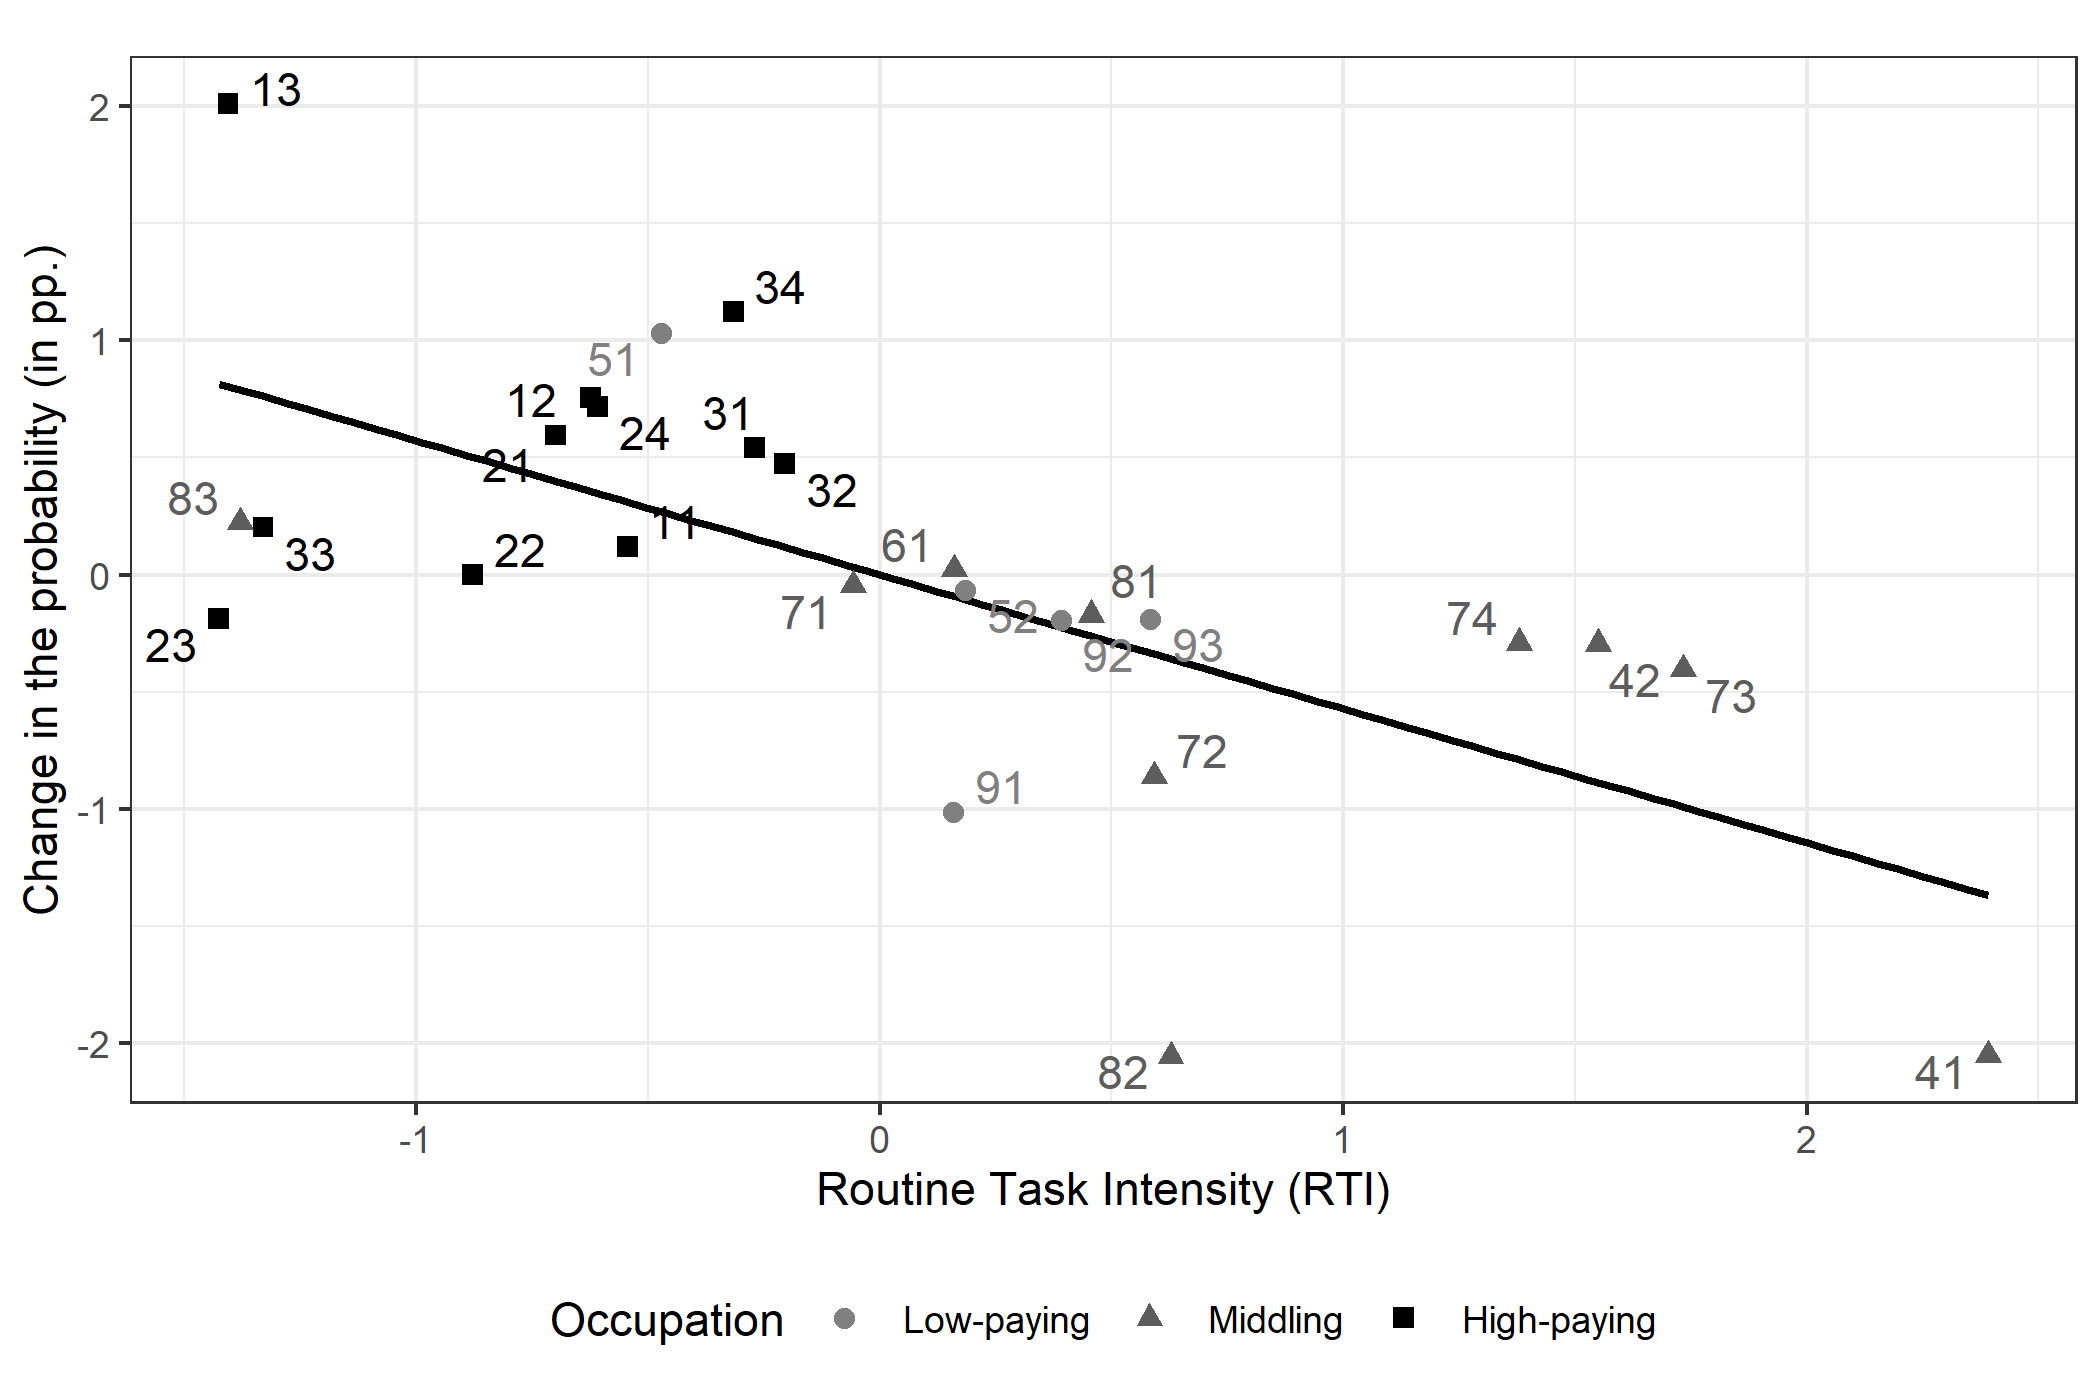
\includegraphics[width=\linewidth]{chap2/graphic/polarize-rtiLIS-p3.png}
	\vspace{-3em}
	\justify\singlespacing\footnotesize{\textit{Notes:} This figure shows the negative relationship between the difference, expressed in percentage points, between the BCS70 and NCDS58 cohorts in terms of probability of being in each ISCO-88 occupation in second period and the Routine Task Intensity (RTI) index from \cite{Mahutga2018Job}.}
\end{figure}

Lastly, Figure \ref{chap2-fig:lfs-change} reports the change in polarization in each of the regions obtained from the LFS.  

\begin{figure}[!htb]
    \centering
    \caption{Between-cohort change in the average share of total employment over the lifecycle of both cohorts (at the regional level)}
    \label{chap2-fig:lfs-change}
    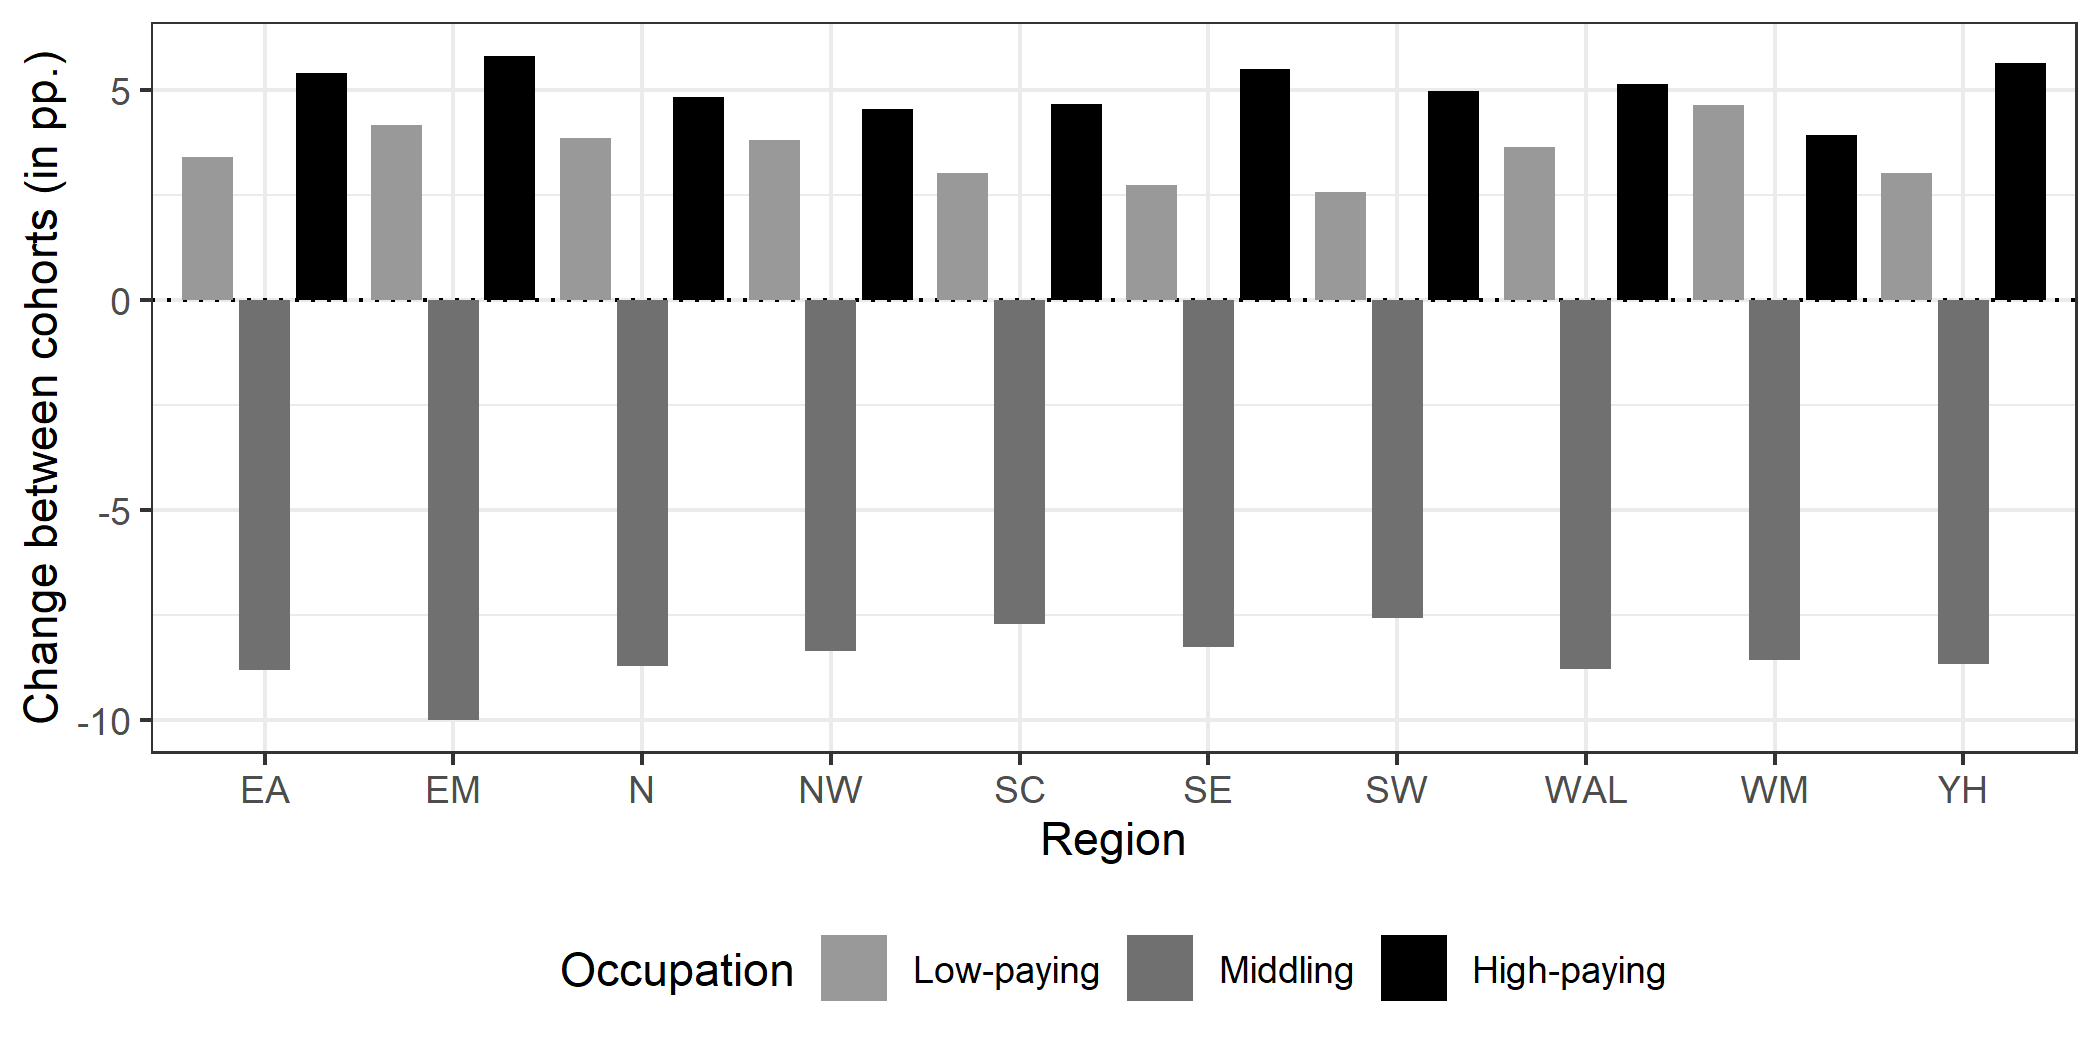
\includegraphics[width=\linewidth]{chap2/graphic/lfs-change.png}
	\vspace{-3em}
	\justify\singlespacing\footnotesize{\textit{Notes:} This figure presents the job polarization at the regional level using the Labour Force Survey data from 1981 to 2012.}
\end{figure}
    \clearpage
    \subsection{Logistic regressions}\label{chap2-app-logit}
    This appendix provides the regression tables for occupations under the multinomial and the binomial specifications of the logistic regressions. We also discuss the complementarity of both specifications to interpret coefficients as the the multinomial coefficients are relative to the baseline occupation category, namely, out-of-work.

\subsubsection{First-period occupation}

Table \ref{chap2-tab:occ-multi1-base} reports the coefficients of the \emph{multinomial} logistic regression from equation \eqref{chap2-eq:emp-multi1} for the first-period occupation. Table \ref{chap2-tab:occ-bi1-base} reports the coefficients regressions for the equivalent \emph{binomial} specification.

Each of these two estimation methods has advantages and disadvantages. Consider first the binomial logit in Table \ref{chap2-tab:occ-bi1-base}. Each regression compares the probability of being in occupation $j$ relative to the other three outcomes. In some cases, the regression is easy to interpret. For example, the regression for out-of-work compares this outcome relative to a composite of all three other occupations, i.e. being in employment. The coefficients on the Out-of-work column then tell us that for the NCDS58 cohort parental income had no effect on being out-of-work, while for the BCS70 it had a negative and significant effect. For low-paying occupations we find that parental income reduces the likelihood to be in the occupation, with the effect being three times as high for the BCS70 than for the NCDS58. The 4th column indicates that parental income increases the probability of being in a high-paying occupation (as compared to the other three outcomes) for both cohorts, although the coefficient is twice as high for the younger cohort. The interpretation of the regressions becomes harder for middling occupations as the alternative not-being-in-middling-occupations includes outcomes that are better and outcomes that are worse than middling. We find a moderate effect of parental income (-0.07) and no significant change across cohorts. Yet this may be the result of differential effects for moving up or down the occupational scale.

A solution to the above problem is to consider a multinomial logit, which compares the likelihood to be in each of the three employment categories to that of the reference group, out-of-work. The multinomial regressions have the advantage of considering simultaneously all the possible outcomes, yet they are harder to interpret as the coefficients represent odds relative to the omitted group. That is, when considering coefficients one needs to keep in mind the dynamics for the out-of-work outcome as captured by the Out-of-work column in Table \ref{chap2-tab:occ-bi1-base}. 

The results for the multinomial estimation reported in Table \ref{chap2-tab:occ-multi1-base} indicate that the likelihood to be in a high-paying occupation is strongly affected by parental income, with the coefficient doubling across cohorts (from 0.21 to 0.42). The insignificant coefficients on ``$\text{Par. Inc.}$'' indicate that, for the NCDS58 cohort, parental income does not give an advantage to get low-paying or middling jobs relative to being out of work. However, it does confer such an advantage for the younger cohort. The negative slopes reported in Figure \ref{chap2-fig:occ-multi1-pinc} are the combination of a large decline in the coefficient on parental income for those out-of-work (see the coefficient on ``$\text{Par. inc.}~\times~\text{BCS}$'' in the first column in Table \ref{chap2-tab:occ-bi1-base}) and the positive but smaller coefficients on the first two columns of Table \ref{chap2-tab:occ-multi1-base}.

\begin{table}[!htb]
    \centering
    \caption{Probability of being in each occupation at first period (multinomial)}
    \label{chap2-tab:occ-multi1-base}
    \begin{threeparttable}
        \centering
        \setlength{\tabcolsep}{15pt}
        \begin{tabular}{l D{.}{.}{5.5} D{.}{.}{5.5} D{.}{.}{5.5}}
\toprule
 & \multicolumn{3}{c}{Multinomial logit - Dep. var.: First-period occupation} \\
\cmidrule(lr){2-4}
 & \multicolumn{1}{c}{Low-paying} & \multicolumn{1}{c}{Middling} & \multicolumn{1}{c}{High-paying} \\
\midrule
Intercept              & 0.08        & 1.39^{***}  & 0.69^{***}  \\
                       & (0.07)      & (0.06)      & (0.06)      \\
BCS cohort             & 0.24^{**}   & 0.12        & 0.75^{***}  \\
                       & (0.10)      & (0.08)      & (0.09)      \\
Female                 & -0.79^{***} & -1.27^{***} & -0.99^{***} \\
                       & (0.09)      & (0.07)      & (0.08)      \\
Female $\times$ BCS    & 0.25^{**}   & -0.02       & -0.08       \\
                       & (0.12)      & (0.10)      & (0.11)      \\
Par. inc.              & -0.03       & -0.00       & 0.21^{***}  \\
                       & (0.04)      & (0.03)      & (0.04)      \\
Par. inc. $\times$ BCS & 0.10^{*}    & 0.22^{***}  & 0.41^{***}  \\
                       & (0.06)      & (0.05)      & (0.05)      \\
\midrule
Num. obs. & \multicolumn{1}{c}{14763} & \multicolumn{1}{c}{14763} & \multicolumn{1}{c}{14763}\\
\bottomrule
\end{tabular}

        \begin{tablenotes}[flushleft]
            \footnotesize{\item \textit{Notes}: 
            % Stars and SE
            $^{***}p<0.01$; $^{**}p<0.05$; $^{*}p<0.1$. Standard errors between parentheses. 
            % Baseline outcome
            Out-of-work occupation in first period is the base outcome of the multinomial logistic regression.
            % Referent group
            Male in the NCDS58 cohort is the referent group. 
            % Variables details
            Parental income in logarithm and then standardized at the cohort level.}
        \end{tablenotes}
    \end{threeparttable}
\end{table}

\begin{table}[!htb]
    \centering
    \caption{Probability of being in each occupation at first period (binomial)}
    \label{chap2-tab:occ-bi1-base}
    \begin{threeparttable}
        \centering
        % \setlength{\tabcolsep}{0pt}
        \begin{tabular}{l D{.}{.}{5.5} D{.}{.}{5.5} D{.}{.}{5.5} D{.}{.}{5.5}}
\toprule
 & \multicolumn{4}{c}{Binomial logit - Dep. var.: First-period occupation} \\
\cmidrule(lr){2-5}
 & \multicolumn{1}{c}{Out-of-work} & \multicolumn{1}{c}{Low-paying} & \multicolumn{1}{c}{Middling} & \multicolumn{1}{c}{High-paying} \\
\midrule
Intercept              & -1.96^{***} & -1.87^{***} & -0.02       & -1.12^{***} \\
                       & (0.05)      & (0.05)      & (0.03)      & (0.04)      \\
BCS cohort             & -0.37^{***} & -0.11       & -0.39^{***} & 0.62^{***}  \\
                       & (0.08)      & (0.07)      & (0.05)      & (0.05)      \\
Female                 & 1.10^{***}  & 0.10        & -0.67^{***} & -0.14^{**}  \\
                       & (0.06)      & (0.07)      & (0.05)      & (0.06)      \\
Female $\times$ BCS    & -0.04       & 0.31^{***}  & 0.08        & -0.10       \\
                       & (0.09)      & (0.10)      & (0.07)      & (0.07)      \\
Par. inc.              & -0.05       & -0.08^{**}  & -0.07^{***} & 0.22^{***}  \\
                       & (0.03)      & (0.03)      & (0.02)      & (0.03)      \\
Par. inc. $\times$ BCS & -0.29^{***} & -0.17^{***} & -0.04       & 0.27^{***}  \\
                       & (0.04)      & (0.04)      & (0.03)      & (0.04)      \\
\midrule
Pseudo R$^2$ & \multicolumn{1}{c}{0.05} & \multicolumn{1}{c}{0.01} & \multicolumn{1}{c}{0.02} & \multicolumn{1}{c}{0.04}\\
Log Likelihood & \multicolumn{1}{c}{-6687.29} & \multicolumn{1}{c}{-6085.09} & \multicolumn{1}{c}{-9482.35} & \multicolumn{1}{c}{-8664.53}\\
Num. obs. & \multicolumn{1}{c}{14763} & \multicolumn{1}{c}{14763} & \multicolumn{1}{c}{14763} & \multicolumn{1}{c}{14763}\\
\bottomrule
\end{tabular}

        \begin{tablenotes}[flushleft]
            \footnotesize{\item \textit{Notes}: 
            % Stars and SE
            $^{***}p<0.01$; $^{**}p<0.05$; $^{*}p<0.1$. Standard errors between parentheses. 
            % Referent group
            Male in the NCDS58 cohort is the referent group. 
            % Variables details
            Parental income in logarithm and then standardized at the cohort level.}
        \end{tablenotes}
    \end{threeparttable}
\end{table}

\subsubsection{Second-period occupation}

Table \ref{chap2-tab:occ-multi23-base} reports the coefficients of the \emph{multinomial} logistic regression for second-period occupation. Table \ref{chap2-tab:occ-bi23-base} reports the coefficients regressions for the equivalent \emph{binomial} specification.

The first three columns report the coefficients for the baseline regression discussed in the text. The next three consider the role played by initial occupation. For the interpretation of the impact of the first period occupations, we have to keep in mind that the omitted group are those out of work. Thus absolute coefficients are the difference in log-odds with respect to out-of-work young individuals (middle panel) and the coefficients for BCS70 indicate the change in the log-odds between both cohorts (bottom panel). The positive coefficients in the second panel indicate that being in either of these occupations when young increases the probability of being in employment at age 42. The figures display a considerable degree of persistence, with the coefficients on the diagonal being large and highly significant. Note that being in a middling-occupation when young implies not only a high probability of being in that occupation when mature (coefficient of 1.47) but also a high probability of moving to a high-paying occupation (coefficient of 0.82). 

When we compare the impact of initial occupation across the cohorts (bottom panel) there are only two significant changes. First, we see a considerable improvement in the outcomes for those who started in a low-paying occupation, for whom the odds of being out-of-work fell for the younger cohort. Second, for those who started in middling occupations, persistence increased considerably. This contrasts with the finding that persistence did not increase for those in high-paying occupations. 


\begin{table}[!htb]
    \centering
    \caption{Probability of being in each occupation in the second period (multinomial)}
    \label{chap2-tab:occ-multi23-base}
    \resizebox*{\textwidth}{!}{
    \begin{threeparttable}
        \setlength{\tabcolsep}{0pt}
        \begin{tabular}{l D{.}{.}{5.5} D{.}{.}{5.5} D{.}{.}{5.5} D{.}{.}{5.5} D{.}{.}{5.5} D{.}{.}{5.5}}
\toprule
 & \multicolumn{6}{c}{Multinomial logit - Dep. var.: Second-period occupation} \\
\cmidrule(lr){2-7}
 & \multicolumn{3}{c}{(1)} & \multicolumn{3}{c}{(2)} \\
\cmidrule(lr){2-4}\cmidrule(lr){5-7}
 & \multicolumn{1}{c}{Low} & \multicolumn{1}{c}{Mid} & \multicolumn{1}{c}{High} & \multicolumn{1}{c}{Low} & \multicolumn{1}{c}{Mid} & \multicolumn{1}{c}{High} \\
\midrule
Intercept                                                                          & 0.38^{***} & 1.37^{***}  & 1.69^{***}  & -0.10      & 0.44^{***}  & 0.81^{***}  \\
                                                                                   & (0.08)     & (0.07)      & (0.07)      & (0.11)     & (0.10)      & (0.10)      \\
BCS cohort                                                                         & 0.04       & -0.04       & 0.11        & -0.07      & -0.46^{***} & -0.32^{**}  \\
                                                                                   & (0.11)     & (0.09)      & (0.09)      & (0.15)     & (0.15)      & (0.14)      \\
Female                                                                             & -0.13      & -1.23^{***} & -1.23^{***} & -0.01      & -0.98^{***} & -1.13^{***} \\
                                                                                   & (0.09)     & (0.08)      & (0.08)      & (0.10)     & (0.09)      & (0.09)      \\
Female $\times$ BCS                                                                & -0.04      & -0.12       & 0.16        & -0.11      & -0.09       & 0.25^{**}   \\
                                                                                   & (0.13)     & (0.12)      & (0.11)      & (0.13)     & (0.12)      & (0.12)      \\
Par. inc.                                                                          & 0.01       & 0.04        & 0.19^{***}  & 0.02       & 0.05        & 0.14^{***}  \\
                                                                                   & (0.04)     & (0.04)      & (0.04)      & (0.04)     & (0.04)      & (0.04)      \\
Par. inc. $\times$ BCS                                                             & 0.05       & 0.15^{***}  & 0.36^{***}  & 0.05       & 0.11^{**}   & 0.25^{***}  \\
                                                                                   & (0.06)     & (0.05)      & (0.05)      & (0.06)     & (0.06)      & (0.05)      \\
\midrule\multicolumn{7}{l}{Change with respect to the referent group as first period occupation (Out-of-work)} \\ \midrule
\quad Low-paying                                                                   &            &             &             & 1.00^{***} & 0.31^{**}   & 0.14        \\
                                                                                   &            &             &             & (0.12)     & (0.13)      & (0.13)      \\
\quad Middling                                                                     &            &             &             & 0.50^{***} & 1.47^{***}  & 0.82^{***}  \\
                                                                                   &            &             &             & (0.11)     & (0.10)      & (0.10)      \\
\quad High-paying                                                                  &            &             &             & 0.06       & 0.52^{***}  & 1.96^{***}  \\
                                                                                   &            &             &             & (0.14)     & (0.14)      & (0.12)      \\
\midrule\multicolumn{7}{l}{Change between cohorts} \\ \midrule
\quad Low. $\times$ BCS                                                            &            &             &             & 0.47^{***} & 0.66^{***}  & 0.55^{***}  \\
                                                                                   &            &             &             & (0.17)     & (0.19)      & (0.18)      \\
\quad Mid. $\times$ BCS                                                            &            &             &             & 0.02       & 0.55^{***}  & 0.25^{*}    \\
                                                                                   &            &             &             & (0.15)     & (0.15)      & (0.15)      \\
\quad High. $\times$ BCS                                                           &            &             &             & 0.17       & 0.37^{**}   & 0.15        \\
                                                                                   &            &             &             & (0.19)     & (0.19)      & (0.16)      \\
\midrule
Num. obs. & \multicolumn{1}{c}{14763} & \multicolumn{1}{c}{14763} & \multicolumn{1}{c}{14763} & \multicolumn{1}{c}{14763} & \multicolumn{1}{c}{14763} & \multicolumn{1}{c}{14763}\\
\bottomrule
\end{tabular}

        \begin{tablenotes}[flushleft]
            \footnotesize{\item\textit{Notes}: 
            % Stars and SE
            $^{***}p<0.01$; $^{**}p<0.05$; $^{*}p<0.1$. Standard errors between parentheses. 
            % Baseline outcome
            Out-of-work occupation in second period is the base outcome of the multinomial logistic regression.
            % Referent group
            Male in the NCDS58 cohort in out-of-work occupation in first period is the referent group. 
            % Variables details
            Parental income in logarithm and then standardized at the cohort level. 
            % Explaining bottom panels
            Coefficients in the first bottom panel captures the change in the marginal effect of the first-period occupation with respect to the referent one, i.e. out-of-work. Coefficients in the second bottom panel indicates the change across cohorts in the marginal effect of the first-period occupation.}
        \end{tablenotes}
    \end{threeparttable}
    }
\end{table}

\begin{table}[!htb]
    \centering
    \caption{Probability of being in each occupation in the second period (binomial)}
    \label{chap2-tab:occ-bi23-base}
    \resizebox*{\textwidth}{!}{
    % \resizebox*{!}{\dimexpr\textheight-2\baselineskip\relax}{
    \begin{threeparttable}
        \setlength{\tabcolsep}{0pt}
        \begin{tabular}{l D{.}{.}{5.5} D{.}{.}{5.5} D{.}{.}{5.5} D{.}{.}{5.5} D{.}{.}{5.5} D{.}{.}{5.5} D{.}{.}{5.5} D{.}{.}{5.5}}
\toprule
 & \multicolumn{8}{c}{Binomial logit - Dep. var.: Second-period occupation} \\
\cmidrule(lr){2-9}
 & \multicolumn{2}{c}{Out-of-work} & \multicolumn{2}{c}{Low-paying} & \multicolumn{2}{c}{Middling} & \multicolumn{2}{c}{High-paying} \\
\cmidrule(lr){2-3}\cmidrule(lr){4-5}\cmidrule(lr){6-7}\cmidrule(lr){8-9}
 & \multicolumn{1}{c}{(1)} & \multicolumn{1}{c}{(2)} & \multicolumn{1}{c}{(1)} & \multicolumn{1}{c}{(2)} & \multicolumn{1}{c}{(1)} & \multicolumn{1}{c}{(2)} & \multicolumn{1}{c}{(1)} & \multicolumn{1}{c}{(2)} \\
\midrule
Intercept                                                                          & -2.39^{***} & -1.59^{***} & -1.97^{***} & -1.76^{***} & -0.69^{***} & -1.07^{***} & -0.16^{***} & -0.52^{***} \\
                                                                                   & (0.06)      & (0.09)      & (0.05)      & (0.08)      & (0.04)      & (0.08)      & (0.04)      & (0.07)      \\
BCS cohort                                                                         & -0.06       & 0.27^{**}   & -0.02       & 0.13        & -0.15^{***} & -0.33^{***} & 0.12^{**}   & -0.18^{*}   \\
                                                                                   & (0.09)      & (0.12)      & (0.07)      & (0.12)      & (0.05)      & (0.12)      & (0.05)      & (0.10)      \\
Female                                                                             & 0.99^{***}  & 0.80^{***}  & 0.89^{***}  & 0.85^{***}  & -0.51^{***} & -0.39^{***} & -0.61^{***} & -0.66^{***} \\
                                                                                   & (0.08)      & (0.08)      & (0.07)      & (0.07)      & (0.05)      & (0.06)      & (0.05)      & (0.06)      \\
Female $\times$ BCS                                                                & -0.04       & -0.06       & -0.09       & -0.19^{**}  & -0.17^{**}  & -0.17^{**}  & 0.20^{***}  & 0.30^{***}  \\
                                                                                   & (0.10)      & (0.11)      & (0.09)      & (0.10)      & (0.08)      & (0.08)      & (0.07)      & (0.08)      \\
Par. inc.                                                                          & -0.09^{***} & -0.07^{**}  & -0.08^{***} & -0.05       & -0.06^{**}  & -0.03       & 0.17^{***}  & 0.12^{***}  \\
                                                                                   & (0.03)      & (0.03)      & (0.03)      & (0.03)      & (0.03)      & (0.03)      & (0.03)      & (0.03)      \\
Par. inc. $\times$ BCS                                                             & -0.23^{***} & -0.16^{***} & -0.18^{***} & -0.10^{**}  & -0.07^{**}  & -0.04       & 0.28^{***}  & 0.19^{***}  \\
                                                                                   & (0.05)      & (0.05)      & (0.04)      & (0.04)      & (0.04)      & (0.04)      & (0.04)      & (0.04)      \\
\midrule\multicolumn{9}{l}{Change with respect to the referent group as first period occupation (Out-of-work)} \\ \midrule
\quad Low-paying                                                                   &             & -0.54^{***} &             & 0.88^{***}  &             & -0.10       &             & -0.33^{***} \\
                                                                                   &             & (0.11)      &             & (0.09)      &             & (0.10)      &             & (0.10)      \\
\quad Middling                                                                     &             & -0.98^{***} &             & -0.36^{***} &             & 0.97^{***}  &             & -0.03       \\
                                                                                   &             & (0.09)      &             & (0.08)      &             & (0.08)      &             & (0.07)      \\
\quad High-paying                                                                  &             & -1.25^{***} &             & -1.15^{***} &             & -0.71^{***} &             & 1.76^{***}  \\
                                                                                   &             & (0.11)      &             & (0.11)      &             & (0.10)      &             & (0.08)      \\
\midrule\multicolumn{9}{l}{Change between cohorts} \\ \midrule
\quad Low. $\times$ BCS                                                            &             & -0.57^{***} &             & 0.11        &             & 0.26^{*}    &             & 0.13        \\
                                                                                   &             & (0.15)      &             & (0.13)      &             & (0.15)      &             & (0.14)      \\
\quad Mid. $\times$ BCS                                                            &             & -0.26^{**}  &             & -0.18       &             & 0.47^{***}  &             & 0.08        \\
                                                                                   &             & (0.13)      &             & (0.12)      &             & (0.12)      &             & (0.11)      \\
\quad High. $\times$ BCS                                                           &             & -0.22       &             & 0.03        &             & 0.29^{**}   &             & 0.03        \\
                                                                                   &             & (0.14)      &             & (0.15)      &             & (0.14)      &             & (0.11)      \\
\midrule
Pseudo R$^2$ & \multicolumn{1}{c}{0.04} & \multicolumn{1}{c}{0.08} & \multicolumn{1}{c}{0.03} & \multicolumn{1}{c}{0.10} & \multicolumn{1}{c}{0.02} & \multicolumn{1}{c}{0.10} & \multicolumn{1}{c}{0.03} & \multicolumn{1}{c}{0.14}\\
Log Likelihood & \multicolumn{1}{c}{-5771.10} & \multicolumn{1}{c}{-5530.48} & \multicolumn{1}{c}{-6886.99} & \multicolumn{1}{c}{-6378.03} & \multicolumn{1}{c}{-8257.73} & \multicolumn{1}{c}{-7541.67} & \multicolumn{1}{c}{-9679.83} & \multicolumn{1}{c}{-8582.94}\\
Num. obs. & \multicolumn{1}{c}{14763} & \multicolumn{1}{c}{14763} & \multicolumn{1}{c}{14763} & \multicolumn{1}{c}{14763} & \multicolumn{1}{c}{14763} & \multicolumn{1}{c}{14763} & \multicolumn{1}{c}{14763} & \multicolumn{1}{c}{14763}\\
\bottomrule
\end{tabular}

        \begin{tablenotes}[flushleft]
            \footnotesize{\item\textit{Notes}: 
            % Stars and SE
            $^{***}p<0.01$; $^{**}p<0.05$; $^{*}p<0.1$. Standard errors between parentheses. 
            % Referent group
            Male in the NCDS58 cohort in out-of-work occupation in first period is the referent group. 
            % Variables details
            Parental income in logarithm and then standardized at the cohort level. 
            % Explaining bottom panels
            Coefficients in the first bottom panel captures the change in the marginal effect of the first-period occupation with respect to the referent one, i.e. out-of-work. Coefficients in the second bottom panel indicates the change across cohorts in the marginal effect of the first-period occupation.}
        \end{tablenotes}
    \end{threeparttable}
    }
\end{table}
    \clearpage
    \subsection{Accounting for education} \label{chap2-app-education}
    This section replicates our core analysis but considers a three-step process in which we also account for education. We start by estimating the impact of parental income on child education, and consider the following linear specification:
\begin{equation}\label{chap2-eq:emp-educ0}
    E^c = \alpha_4 + \beta_4 Y^p + \phi_f E^f + \phi_m E^m + \gamma_4 X,
\end{equation}
where $E^c$ is the child's education, and $E^f$ (resp. $E^m$) is the father's (resp. mother's) education. Education variables are measured in peer-inclusive downward-looking ranking. All terms are
interacted with a dummy that equals one for those in the 1970 cohort (BCS70).
Table \ref{chap2-tab:educ-linear1} summarizes the coefficients for the determinants of child's education.
\begin{table}[!htb]
    \centering
    \caption{Determinants of child's education}
    \label{chap2-tab:educ-linear1}
    \resizebox*{\textwidth}{!}{
    \begin{threeparttable}
        \centering
        % \setlength{\tabcolsep}{3pt}
        \begin{tabular}{l D{.}{.}{5.5} D{.}{.}{5.5} D{.}{.}{5.5} D{.}{.}{5.5} D{.}{.}{5.5}}
\toprule
 & \multicolumn{5}{c}{Linear regression - Dep. var.: Education (in PIR-STD)} \\
\cmidrule(lr){2-6}
 & \multicolumn{1}{c}{(1)} & \multicolumn{1}{c}{(2)} & \multicolumn{1}{c}{(3)} & \multicolumn{1}{c}{(4)} & \multicolumn{1}{c}{(5)} \\
\midrule
Intercept                        & -0.01      & 0.01        & 0.03^{*}    & -0.16^{***} & -0.21^{***} \\
                                 & (0.01)     & (0.01)      & (0.02)      & (0.04)      & (0.05)      \\
BCS cohort                       & -0.03      & -0.05^{**}  & -0.05^{**}  & -0.11^{***} & -0.05       \\
                                 & (0.02)     & (0.02)      & (0.02)      & (0.02)      & (0.03)      \\
Female                           & 0.07^{***} & 0.06^{***}  & 0.07^{***}  & 0.05^{**}   & 0.05^{**}   \\
                                 & (0.02)     & (0.02)      & (0.02)      & (0.02)      & (0.02)      \\
Female $\times$ BCS              & 0.02       & 0.03        & 0.02        & 0.00        & -0.02       \\
                                 & (0.03)     & (0.03)      & (0.03)      & (0.03)      & (0.04)      \\
Par. inc.                        & 0.13^{***} & 0.08^{***}  & 0.08^{***}  & 0.07^{***}  & 0.07^{***}  \\
                                 & (0.01)     & (0.01)      & (0.01)      & (0.01)      & (0.01)      \\
Father's education               &            & 0.19^{***}  & 0.14^{***}  & 0.09^{***}  & 0.09^{***}  \\
                                 &            & (0.01)      & (0.01)      & (0.01)      & (0.01)      \\
Mother's education               &            & 0.13^{***}  & 0.12^{***}  & 0.10^{***}  & 0.10^{***}  \\
                                 &            & (0.01)      & (0.01)      & (0.01)      & (0.01)      \\
Father's soc. class              &            &             & 0.19^{***}  & 0.13^{***}  & 0.13^{***}  \\
                                 &            &             & (0.01)      & (0.01)      & (0.01)      \\
Number of siblings               &            &             &             &             & -0.06^{***} \\
                                 &            &             &             &             & (0.01)      \\
Eldest child                     &            &             &             &             & 0.07^{***}  \\
                                 &            &             &             &             & (0.03)      \\
Par. inc. $\times$ BCS           & 0.11^{***} & 0.11^{***}  & 0.08^{***}  & 0.05^{**}   & 0.06^{***}  \\
                                 & (0.01)     & (0.02)      & (0.02)      & (0.02)      & (0.02)      \\
Father's educ. $\times$ BCS      &            & -0.10^{***} & -0.07^{***} & -0.04^{*}   & -0.03       \\
                                 &            & (0.02)      & (0.02)      & (0.02)      & (0.02)      \\
Mother's educ. $\times$ BCS      &            & -0.03       & -0.02       & -0.03^{*}   & -0.05^{**}  \\
                                 &            & (0.02)      & (0.02)      & (0.02)      & (0.02)      \\
Father's soc. class $\times$ BCS &            &             & -0.06^{***} & -0.04^{**}  & -0.05^{**}  \\
                                 &            &             & (0.02)      & (0.02)      & (0.02)      \\
Number of siblings $\times$ BCS  &            &             &             &             & 0.08^{***}  \\
                                 &            &             &             &             & (0.02)      \\
Eldest child $\times$ BCS        &            &             &             &             & -0.01       \\
                                 &            &             &             &             & (0.04)      \\
\midrule
Parents' interest in education & \multicolumn{1}{c}{ } & \multicolumn{1}{c}{ } & \multicolumn{1}{c}{ } & \multicolumn{1}{c}{Yes} & \multicolumn{1}{c}{Yes} \\
Region FE & \multicolumn{1}{c}{ } & \multicolumn{1}{c}{ } & \multicolumn{1}{c}{ } & \multicolumn{1}{c}{Yes} & \multicolumn{1}{c}{Yes} \\
\midrule
R$^2$ & \multicolumn{1}{c}{0.04} & \multicolumn{1}{c}{0.09} & \multicolumn{1}{c}{0.11} & \multicolumn{1}{c}{0.18} & \multicolumn{1}{c}{0.18}\\
Adj. R$^2$ & \multicolumn{1}{c}{0.04} & \multicolumn{1}{c}{0.09} & \multicolumn{1}{c}{0.11} & \multicolumn{1}{c}{0.17} & \multicolumn{1}{c}{0.18}\\
Num. obs. & \multicolumn{1}{c}{20722} & \multicolumn{1}{c}{17354} & \multicolumn{1}{c}{13901} & \multicolumn{1}{c}{11814} & \multicolumn{1}{c}{10509}\\
\bottomrule
\end{tabular}

        \begin{tablenotes}[flushleft]
            \footnotesize{\item \textit{Notes}: 
            % Stars and SE
            $^{***}p<0.01$; $^{**}p<0.05$; $^{*}p<0.1$. Standard errors between parentheses. 
            % Referent group
            Male in the NCDS58 cohort is the referent group. 
            % Variables details
            Parental income in logarithm and child education in peer-inclusive ranking, both are standardized at the cohort level.}
        \end{tablenotes}
    \end{threeparttable}
    }
\end{table}

Table \ref{chap2-tab:educ-linear1} reports the coefficients obtained when we run various specifications for the determinants of education. The baseline column simply regresses educational attainment on parental income and gender. As expected, the effect of parental income is strong. Moreover, it almost doubles across the two cohorts, increasing from 0.13 for the older cohort to 0.24 for the BCS. The next four columns sequentially introduce other possible determinant of education such as parental education, father's social class and number of siblings. The effect of parental income is reduced as these controls are added to the regression; however, the doubling of the coefficient on parental income across cohorts remains robust.   

The education of the mother and the father as well as the social class of the latter are all important factors in the child's educational outcome, and much of the effect of income identified in column (1) is capturing the effect of these factors. Interestingly, for the BCS70 cohort the impact of such variables has fallen relative to that found for the NCDS58 (although the coefficients are not always significant). This seems to indicate that across the two cohorts parental income has gained importance and other parental characteristics have lost it in determining a child's education.

We next estimate the multinomial logistic regressions for both first- and second-period occupations---equivalent to equations \eqref{chap2-eq:emp-multi1}, \eqref{chap2-eq:emp-multi2}, and \eqref{chap2-eq:emp-multi3} but introducing child's education as an explanatory variable.  The regressions are reported in tables \ref{chap2-tab:educ-multi1-base} and \ref{chap2-tab:educ-multi23-base} and reproduce the results previously obtained. 

Consider the determinants of an individual's probability to start her career in each of the occupations $j$. Comparing these results with those in Table  \ref{chap2-tab:occ-multi1-base} we see that, as far as high-paying occupations go, much of the effect of parental income occurs through education (or unobserved characteristics correlated with education). When we compare the two cohorts, the most important result is that while the direct effect of parental income has increased across cohorts (by the same magnitude as when we did not control for education), that of education has not. 
\begin{table}[!htb]
    \centering
    \caption{Probability of being in each occupation at first period (multinomial)}
    \label{chap2-tab:educ-multi1-base}
    \begin{threeparttable}
        \centering
        \setlength{\tabcolsep}{15pt}
        \begin{tabular}{l D{.}{.}{5.5} D{.}{.}{5.5} D{.}{.}{5.5}}
\toprule
 & \multicolumn{3}{c}{Multinomial logit - Dep. var.: First-period occupation} \\
\cmidrule(lr){2-4}
 & \multicolumn{1}{c}{Low-paying} & \multicolumn{1}{c}{Middling} & \multicolumn{1}{c}{High-paying} \\
\midrule
Intercept              & -0.00       & 1.38^{***}  & 0.53^{***}  \\
                       & (0.07)      & (0.06)      & (0.06)      \\
BCS cohort             & 0.22^{**}   & 0.11        & 0.88^{***}  \\
                       & (0.10)      & (0.08)      & (0.09)      \\
Female                 & -0.76^{***} & -1.26^{***} & -1.02^{***} \\
                       & (0.09)      & (0.07)      & (0.08)      \\
Female $\times$ BCS    & 0.27^{**}   & 0.01        & -0.12       \\
                       & (0.12)      & (0.10)      & (0.11)      \\
Par. inc.              & -0.01       & 0.00        & 0.10^{***}  \\
                       & (0.04)      & (0.03)      & (0.04)      \\
Par. inc. $\times$ BCS & 0.10        & 0.22^{***}  & 0.36^{***}  \\
                       & (0.06)      & (0.05)      & (0.05)      \\
Education              & -0.28^{***} & -0.02       & 0.77^{***}  \\
                       & (0.05)      & (0.04)      & (0.04)      \\
Education $\times$ BCS & 0.04        & -0.04       & -0.05       \\
                       & (0.07)      & (0.05)      & (0.06)      \\
\midrule
Num. obs. & \multicolumn{1}{c}{14547} & \multicolumn{1}{c}{14547} & \multicolumn{1}{c}{14547}\\
\bottomrule
\end{tabular}

        \begin{tablenotes}[flushleft]
            \footnotesize{\item \textit{Notes}: 
            % Stars and SE
            $^{***}p<0.01$; $^{**}p<0.05$; $^{*}p<0.1$. Standard errors between parentheses. 
            % Baseline outcome
            Out-of-work occupation in first period is the base outcome of the multinomial logistic regression.
            % Referent group
            Male in the NCDS58 cohort is the referent group. 
            % Variables details
            Parental income in logarithm and then standardized at the cohort level.
            Education variables and the father’s social class are defined in peer-inclusive ranking. All variables, except dummies, are standardized at the cohort level to take into account changes in the variance of the variables’ distributions between both cohorts.}
        \end{tablenotes}
    \end{threeparttable}
\end{table}


Concerning the occupation of mature workers, Table \ref{chap2-tab:educ-multi23-base} reports regressions in which it depends on education as well as on parental income and the initial job. The coefficients on initial occupations and on parental income are similar to those obtained in the specification without education. Interestingly, the relative impacts of education and parental income on the likelihood to be in a high-paying occupation have changed across cohorts, with parental income becoming more important  and (our measure of) education less for the BCS70 than for the NCDS58 cohort.

\begin{table}[!htb]
    \centering
    \caption{Probability of being in each occupation in the second period (multinomial)}
    \label{chap2-tab:educ-multi23-base}
    \resizebox*{\textwidth}{!}{
    \begin{threeparttable}
        \setlength{\tabcolsep}{0pt}
        \begin{tabular}{l D{.}{.}{5.5} D{.}{.}{5.5} D{.}{.}{5.5} D{.}{.}{5.5} D{.}{.}{5.5} D{.}{.}{5.5}}
\toprule
 & \multicolumn{6}{c}{Multinomial logit - Dep. var.: Second-period occupation} \\
\cmidrule(lr){2-7}
 & \multicolumn{3}{c}{(1)} & \multicolumn{3}{c}{(2)} \\
\cmidrule(lr){2-4}\cmidrule(lr){5-7}
 & \multicolumn{1}{c}{Low} & \multicolumn{1}{c}{Mid} & \multicolumn{1}{c}{High} & \multicolumn{1}{c}{Low} & \multicolumn{1}{c}{Mid} & \multicolumn{1}{c}{High} \\
\midrule
Intercept                                                                          & 0.28^{***}  & 1.38^{***}  & 1.69^{***}  & -0.19^{*}   & 0.45^{***}  & 0.81^{***}  \\
                                                                                   & (0.08)      & (0.07)      & (0.07)      & (0.11)      & (0.11)      & (0.10)      \\
BCS cohort                                                                         & 0.06        & -0.03       & 0.18^{*}    & -0.00       & -0.39^{**}  & -0.17       \\
                                                                                   & (0.11)      & (0.10)      & (0.10)      & (0.16)      & (0.16)      & (0.14)      \\
Female                                                                             & -0.08       & -1.22^{***} & -1.43^{***} & 0.03        & -0.95^{***} & -1.25^{***} \\
                                                                                   & (0.09)      & (0.09)      & (0.09)      & (0.10)      & (0.09)      & (0.09)      \\
Female $\times$ BCS                                                                & -0.07       & -0.11       & 0.22^{*}    & -0.14       & -0.12       & 0.27^{**}   \\
                                                                                   & (0.13)      & (0.12)      & (0.12)      & (0.13)      & (0.12)      & (0.12)      \\
Par. inc.                                                                          & 0.03        & 0.04        & 0.08^{**}   & 0.04        & 0.05        & 0.07^{*}    \\
                                                                                   & (0.04)      & (0.04)      & (0.04)      & (0.04)      & (0.04)      & (0.04)      \\
Par. inc. $\times$ BCS                                                             & 0.05        & 0.14^{**}   & 0.31^{***}  & 0.04        & 0.09        & 0.22^{***}  \\
                                                                                   & (0.06)      & (0.06)      & (0.05)      & (0.06)      & (0.06)      & (0.06)      \\
Education                                                                          & -0.20^{***} & 0.02        & 0.97^{***}  & -0.17^{***} & -0.01       & 0.81^{***}  \\
                                                                                   & (0.05)      & (0.05)      & (0.04)      & (0.05)      & (0.05)      & (0.05)      \\
Education $\times$ BCS                                                             & -0.01       & -0.02       & -0.21^{***} & 0.02        & 0.05        & -0.21^{***} \\
                                                                                   & (0.07)      & (0.06)      & (0.06)      & (0.07)      & (0.07)      & (0.06)      \\
\midrule\multicolumn{7}{l}{Change with respect to the referent group as first period occupation (Out-of-work)} \\ \midrule
\quad Low-paying                                                                   &             &             &             & 0.98^{***}  & 0.29^{**}   & 0.33^{**}   \\
                                                                                   &             &             &             & (0.12)      & (0.14)      & (0.14)      \\
\quad Middling                                                                     &             &             &             & 0.52^{***}  & 1.44^{***}  & 0.90^{***}  \\
                                                                                   &             &             &             & (0.11)      & (0.10)      & (0.11)      \\
\quad High-paying                                                                  &             &             &             & 0.13        & 0.48^{***}  & 1.62^{***}  \\
                                                                                   &             &             &             & (0.15)      & (0.14)      & (0.12)      \\
\midrule\multicolumn{7}{l}{Change between cohorts} \\ \midrule
\quad Low. $\times$ BCS                                                            &             &             &             & 0.41^{**}   & 0.61^{***}  & 0.41^{**}   \\
                                                                                   &             &             &             & (0.17)      & (0.19)      & (0.19)      \\
\quad Mid. $\times$ BCS                                                            &             &             &             & -0.02       & 0.52^{***}  & 0.19        \\
                                                                                   &             &             &             & (0.16)      & (0.15)      & (0.15)      \\
\quad High. $\times$ BCS                                                           &             &             &             & 0.13        & 0.33^{*}    & 0.18        \\
                                                                                   &             &             &             & (0.19)      & (0.19)      & (0.16)      \\
\midrule
Num. obs. & \multicolumn{1}{c}{14547} & \multicolumn{1}{c}{14547} & \multicolumn{1}{c}{14547} & \multicolumn{1}{c}{14547} & \multicolumn{1}{c}{14547} & \multicolumn{1}{c}{14547}\\
\bottomrule
\end{tabular}

        \begin{tablenotes}[flushleft]
            \footnotesize{\item\textit{Notes}: 
            % Stars and SE
            $^{***}p<0.01$; $^{**}p<0.05$; $^{*}p<0.1$. Standard errors between parentheses. 
            % Baseline outcome
            Out-of-work occupation in second period is the base outcome of the multinomial logistic regression.
            % Referent group
            Male in the NCDS58 cohort in out-of-work occupation in first period is the referent group.  
            % Variables details
            Parental income in logarithm and child education in peer-inclusive ranking, both are standardized at the cohort level.
            % Explaining bottom panels
            Coefficients in the first bottom panel captures the change in the marginal effect of the first-period occupation with respect to the referent one, i.e. out-of-work. Coefficients in the second bottom panel indicates the change across cohorts in the marginal effect of the first-period occupation.}
        \end{tablenotes}
    \end{threeparttable}
    }
\end{table}
Overall, these three tables indicate that including education in the analysis has little impact on our estimates of the differences in the parental income coefficients across the to cohorts.

    \clearpage
    \subsection{Additional material}\label{chap2-app-additional}
    This appendix provides various additional figures and tables to complete the analysis.

\subsubsection{Occupational outcomes at age 42}

This subsection provides additional results concerning the outcomes for individuals at age 42. We first provide an alternative depiction of the results provided in Figure \ref{chap2-fig:occ-multi2-pinc} to further illustrate the relationship between parental income and occupational dynamics. Figure \ref{chap2-fig:occ-multi2-quant-male} reports the \emph{change} across the two cohorts in the probability of being in each occupational category at age 42. For each decile in the parental-income distribution, we report the probabilities of being in each of the four occupations, when using the estimates in Table \ref{chap2-tab:occ-multi2-short}. The figure hence indicates how the probability of being in, say, a high-paying occupation for the cohort born in 1970 has changed for a particular parental-income decile relative to what that probability was for those born in 1958. 

\begin{figure}[!tb]
    \centering
    \caption{Change across cohorts in the probability of being in each occupation at age 42 (in percentage points)}
    \label{chap2-fig:occ-multi2-quant-male}
    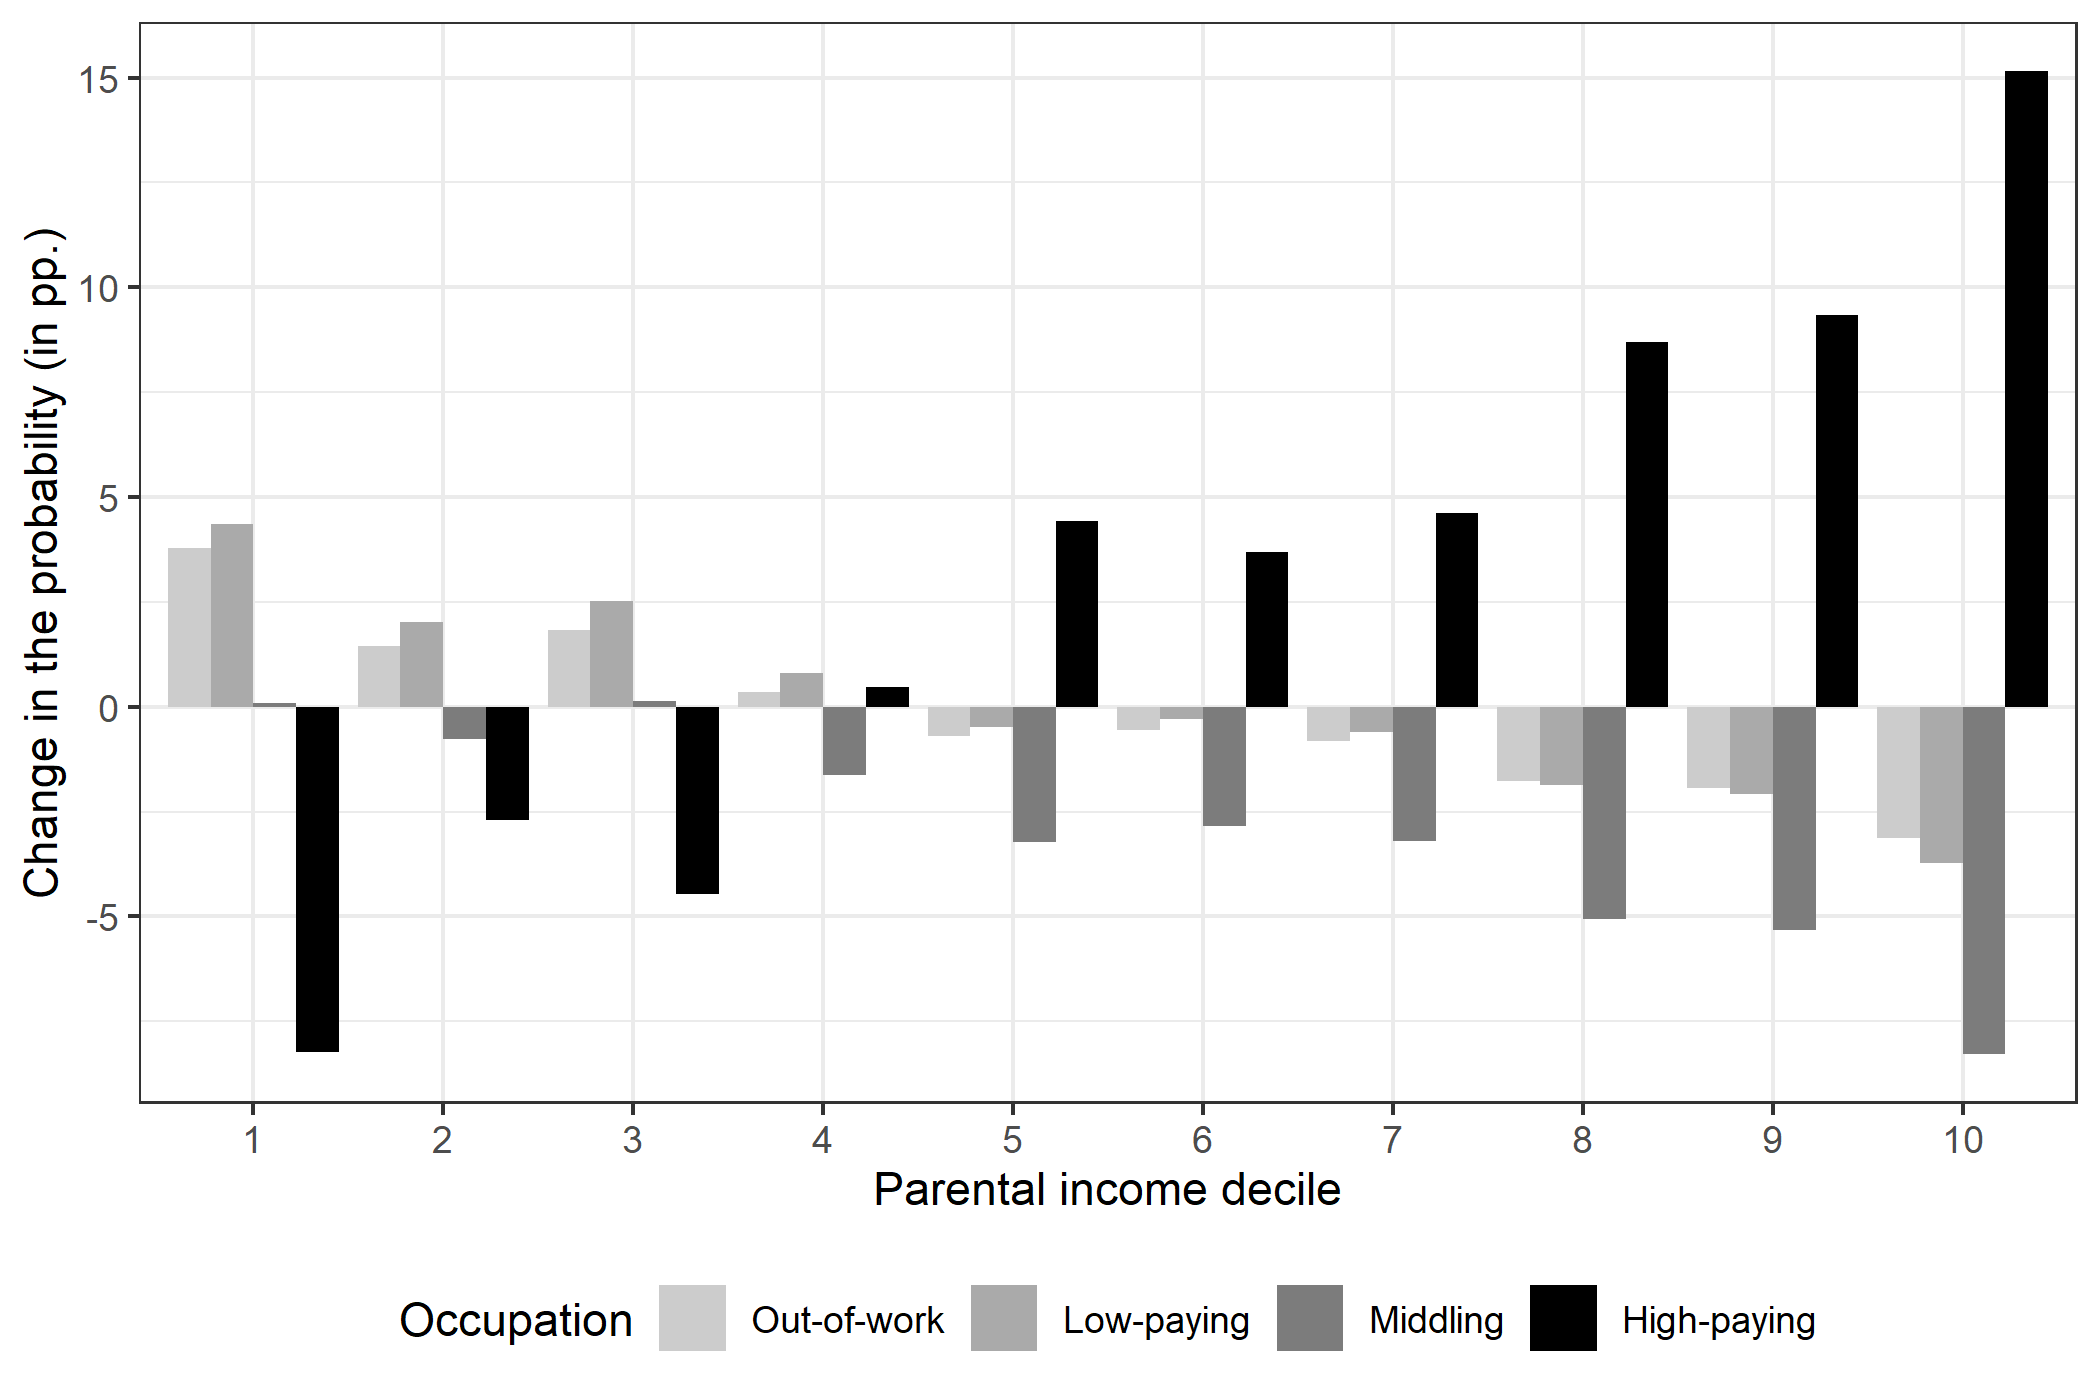
\includegraphics[width=\linewidth]{chap2/graphic/occ-multi2-quant-male.png}
 	\vspace{-3em}
 	\justify\singlespacing\footnotesize{\textit{Notes:} This figure shows the difference, expressed in percentage points, between the BCS70 and NCDS58 cohorts in terms of probability of being in each type of occupation (out-of-work, low-paying, middling, high-paying) at age 42 according to the decile of the parental income distribution. 
 	Probabilities are computed for males in both cohorts at each parental income decile, according to the multinomial logistic regression reported in columns (1) of Table \ref{chap2-tab:occ-multi23-base}.}
 \end{figure}
 
Not surprisingly, for almost all parental-income categories the likelihood of being in a middling job has declined for the younger cohort. The exception are those in the first and third deciles, for whom there has been a small increase. Yet, whether this decline is offset by an increase in the probability of working in a low- or a high-paying occupation is strongly dependent on parental income. It is only for those in the fourth decile that we see the pattern observed in the aggregate data: a reduction in the share of middling jobs accompanied by an increase in that of both low- and high-paying ones. Everywhere else in the distribution the changes in the share of high- and low-paying occupations are of opposite sign. For those in the top half of the parental-income distribution, the decline in the share of middling occupations has been accompanied by lower shares of individuals in both low-paying jobs and out of work and a higher share in high-paying occupations. The magnitude of these changes increases with parental income. For those in the top decile, the proportion of individuals in high-paying jobs rose by 15.1 pp., while that of those in middling fell by 8.3 pp. The bottom three deciles display an increase for out-of-work and low-paying and a decline for high-paying, irrespective of whether there was a positive or negative change in the share of middling jobs, though the magnitudes for the latter are small an all three cases.

Figure \ref{chap2-fig:occ-multi3-pinc-female} provides the change in the probability of being in each occupation in the second period conditional on first-period occupation at several points of the parental income distribution for females. 

\begin{figure}[!htb]
    \centering
    \caption{Change in probability to be in each occupation in the second period according to the first-period occupation and parental income (female only)}
    \label{chap2-fig:occ-multi3-pinc-female}
    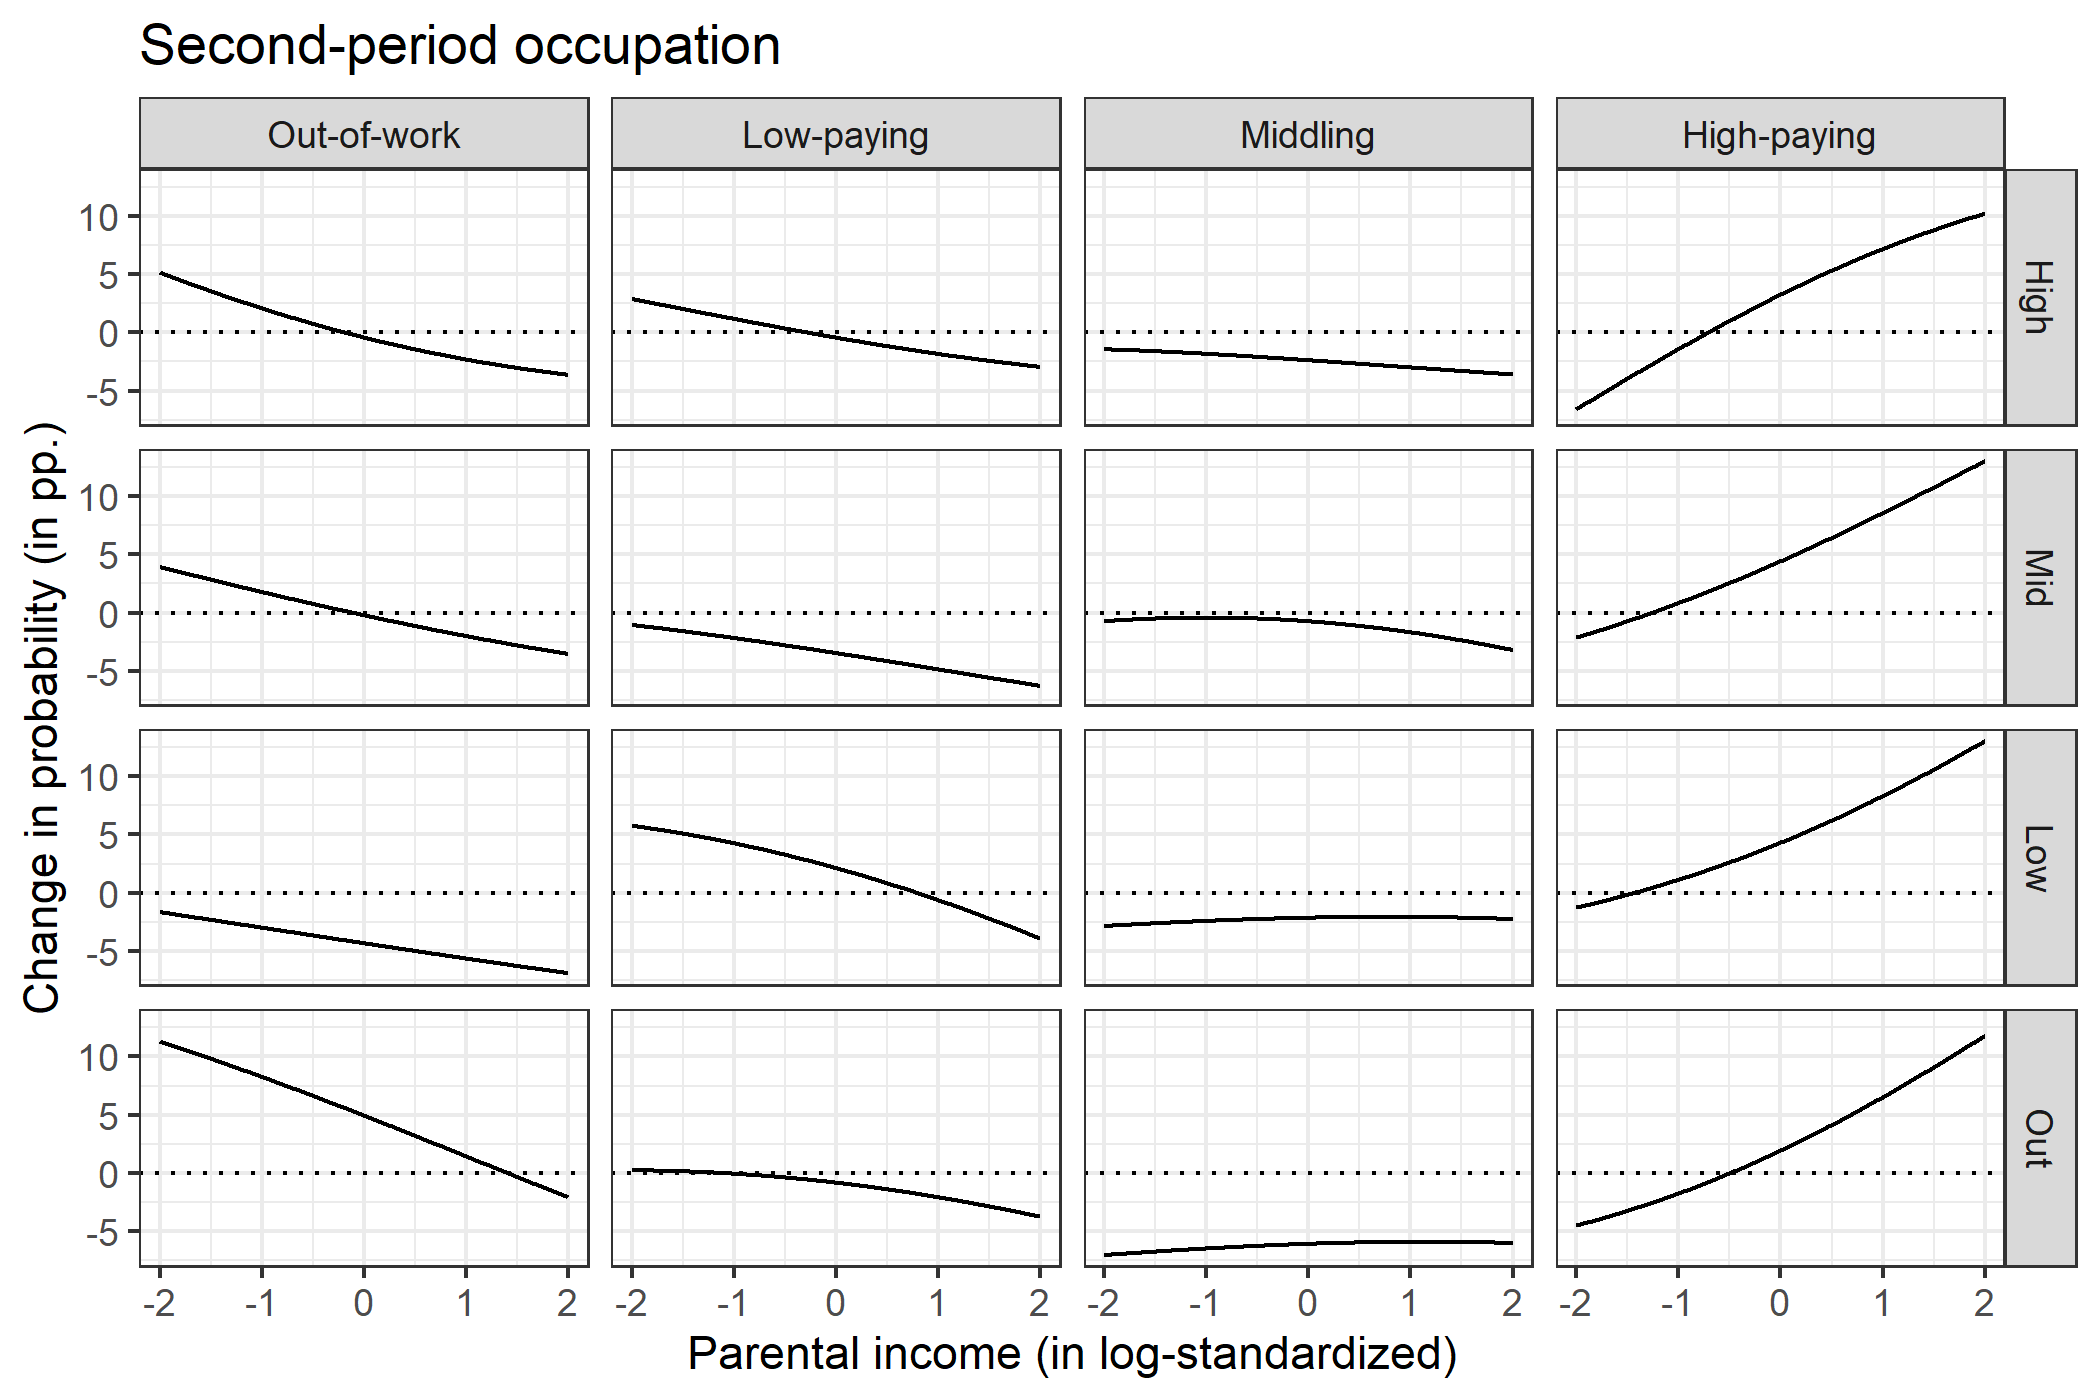
\includegraphics[width=\linewidth]{chap2/graphic/occ-multi3-pinc-female.png}
    \vspace{-3em}
    \justify\singlespacing\footnotesize{\textit{Notes:} This figure presents the difference, expressed in percentage points, between the BCS70 and the NCDS58 cohorts in terms of probability of being in each type of second-period occupation (out-of-work, low-paying, middling, high-paying), conditional on the first-period occupation, according to parental income, in log-standardized.
    Probabilities are computed for females in both cohorts according to the multinomial logistic regression reported in columns (2) of Table \ref{chap2-tab:occ-multi23-base}.}
\end{figure}

We summarize the results on transition probabilities in Table \ref{chap2-tab:mob-pinc-both}. The table reports changes in the probability of each type of mobility depending on the individual’s initial occupation, assessed at several points of the parental income distribution as in the graphs above. The left panel of the table provides the results for men, the right panel for women.
\begin{table}[!tb]
    \centering
    \caption{Change in intra-generational mobility across cohorts}
    \label{chap2-tab:mob-pinc-both}
    \begin{threeparttable}
        \setlength{\tabcolsep}{9pt}
        
\begin{tabular}{lrrrrrr}
\toprule
\multicolumn{1}{c}{} & \multicolumn{3}{c}{Male} & \multicolumn{3}{c}{Female} \\
\cmidrule(l{3pt}r{3pt}){2-4} \cmidrule(l{3pt}r{3pt}){5-7}
First-period occupation & Down & Persist & Up & Down & Persist & Up\\
\midrule
& \multicolumn{3}{c}{\textit{at +2 STD}} & \multicolumn{3}{c}{\textit{at +2 STD}}\\ 
\midrule
Out-of-work &  & -0.57 & 0.57 &  & -2.05 & 2.05\\
Low-paying & -4.41 & -0.88 & 5.29 & -6.88 & -3.90 & 10.78\\
Middling & -3.84 & -0.52 & 4.36 & -9.82 & -3.20 & 13.02\\
High-paying & -2.95 & 2.95 &  & -10.19 & 10.19 & \\
\midrule 
 & \multicolumn{3}{c}{\textit{at the Mean}} & \multicolumn{3}{c}{\textit{at the Mean}}\\ 
\midrule
Out-of-work &  & 4.92 & -4.92 &  & 4.96 & -4.96\\
Low-paying & -2.70 & 4.83 & -2.13 & -4.32 & 2.14 & 2.18\\
Middling & -0.70 & 3.65 & -2.95 & -3.68 & -0.74 & 4.42\\
High-paying & 2.54 & -2.54 &  & -3.25 & 3.25 & \\
\midrule 
 & \multicolumn{3}{c}{\textit{at -2 STD}} & \multicolumn{3}{c}{\textit{at -2 STD}}\\ 
\midrule
Out-of-work &  & 11.27 & -11.27 &  & 11.30 & -11.30\\
Low-paying & -0.53 & 9.57 & -9.04 & -1.65 & 5.76 & -4.11\\
Middling & 3.29 & 5.41 & -8.70 & 2.87 & -0.74 & -2.14\\
High-paying & 10.92 & -10.92 &  & 6.58 & -6.58 & \\
\bottomrule
\end{tabular}

            \begin{tablenotes}[flushleft]
                \footnotesize{\item \textit{Notes}: This Table summarizes the difference, expressed in percentage points, between the BCS70 and the NCDS58 cohorts in terms of type of mobility (down, persist, up) conditional on first period occupation (out-of-work, low-paying, middling, high-paying) at several points of the parental income distribution (at +2 std., at the mean, at -2 std.). These values are computed from the results obtained in Figure \ref{chap2-fig:occ-multi3-pinc-male} for males and in Figure \ref{chap2-fig:occ-multi3-pinc-female} for females.}
            \end{tablenotes}
    \end{threeparttable}
\end{table}

\subsubsection{Results at the regional level}\label{chap2-app-additional-regional}

Figures \ref{chap2-fig:reg-multi2-pinc-male} and \ref{chap2-fig:reg-multi2-pinc-female} depict the probabilities of being in each second period occupation according to parental income at the regional level, for men and women respectively. Figure  \ref{chap2-fig:regocc-absolute-all} depicts the correlation between the change in the parental income coefficient for second-period occupations and the change in job polarization at the regional level.

\begin{figure}[!htb]
    \centering
    \caption{Second-period occupation probability according to parental income at the regional level (male only)}
    \label{chap2-fig:reg-multi2-pinc-male}
    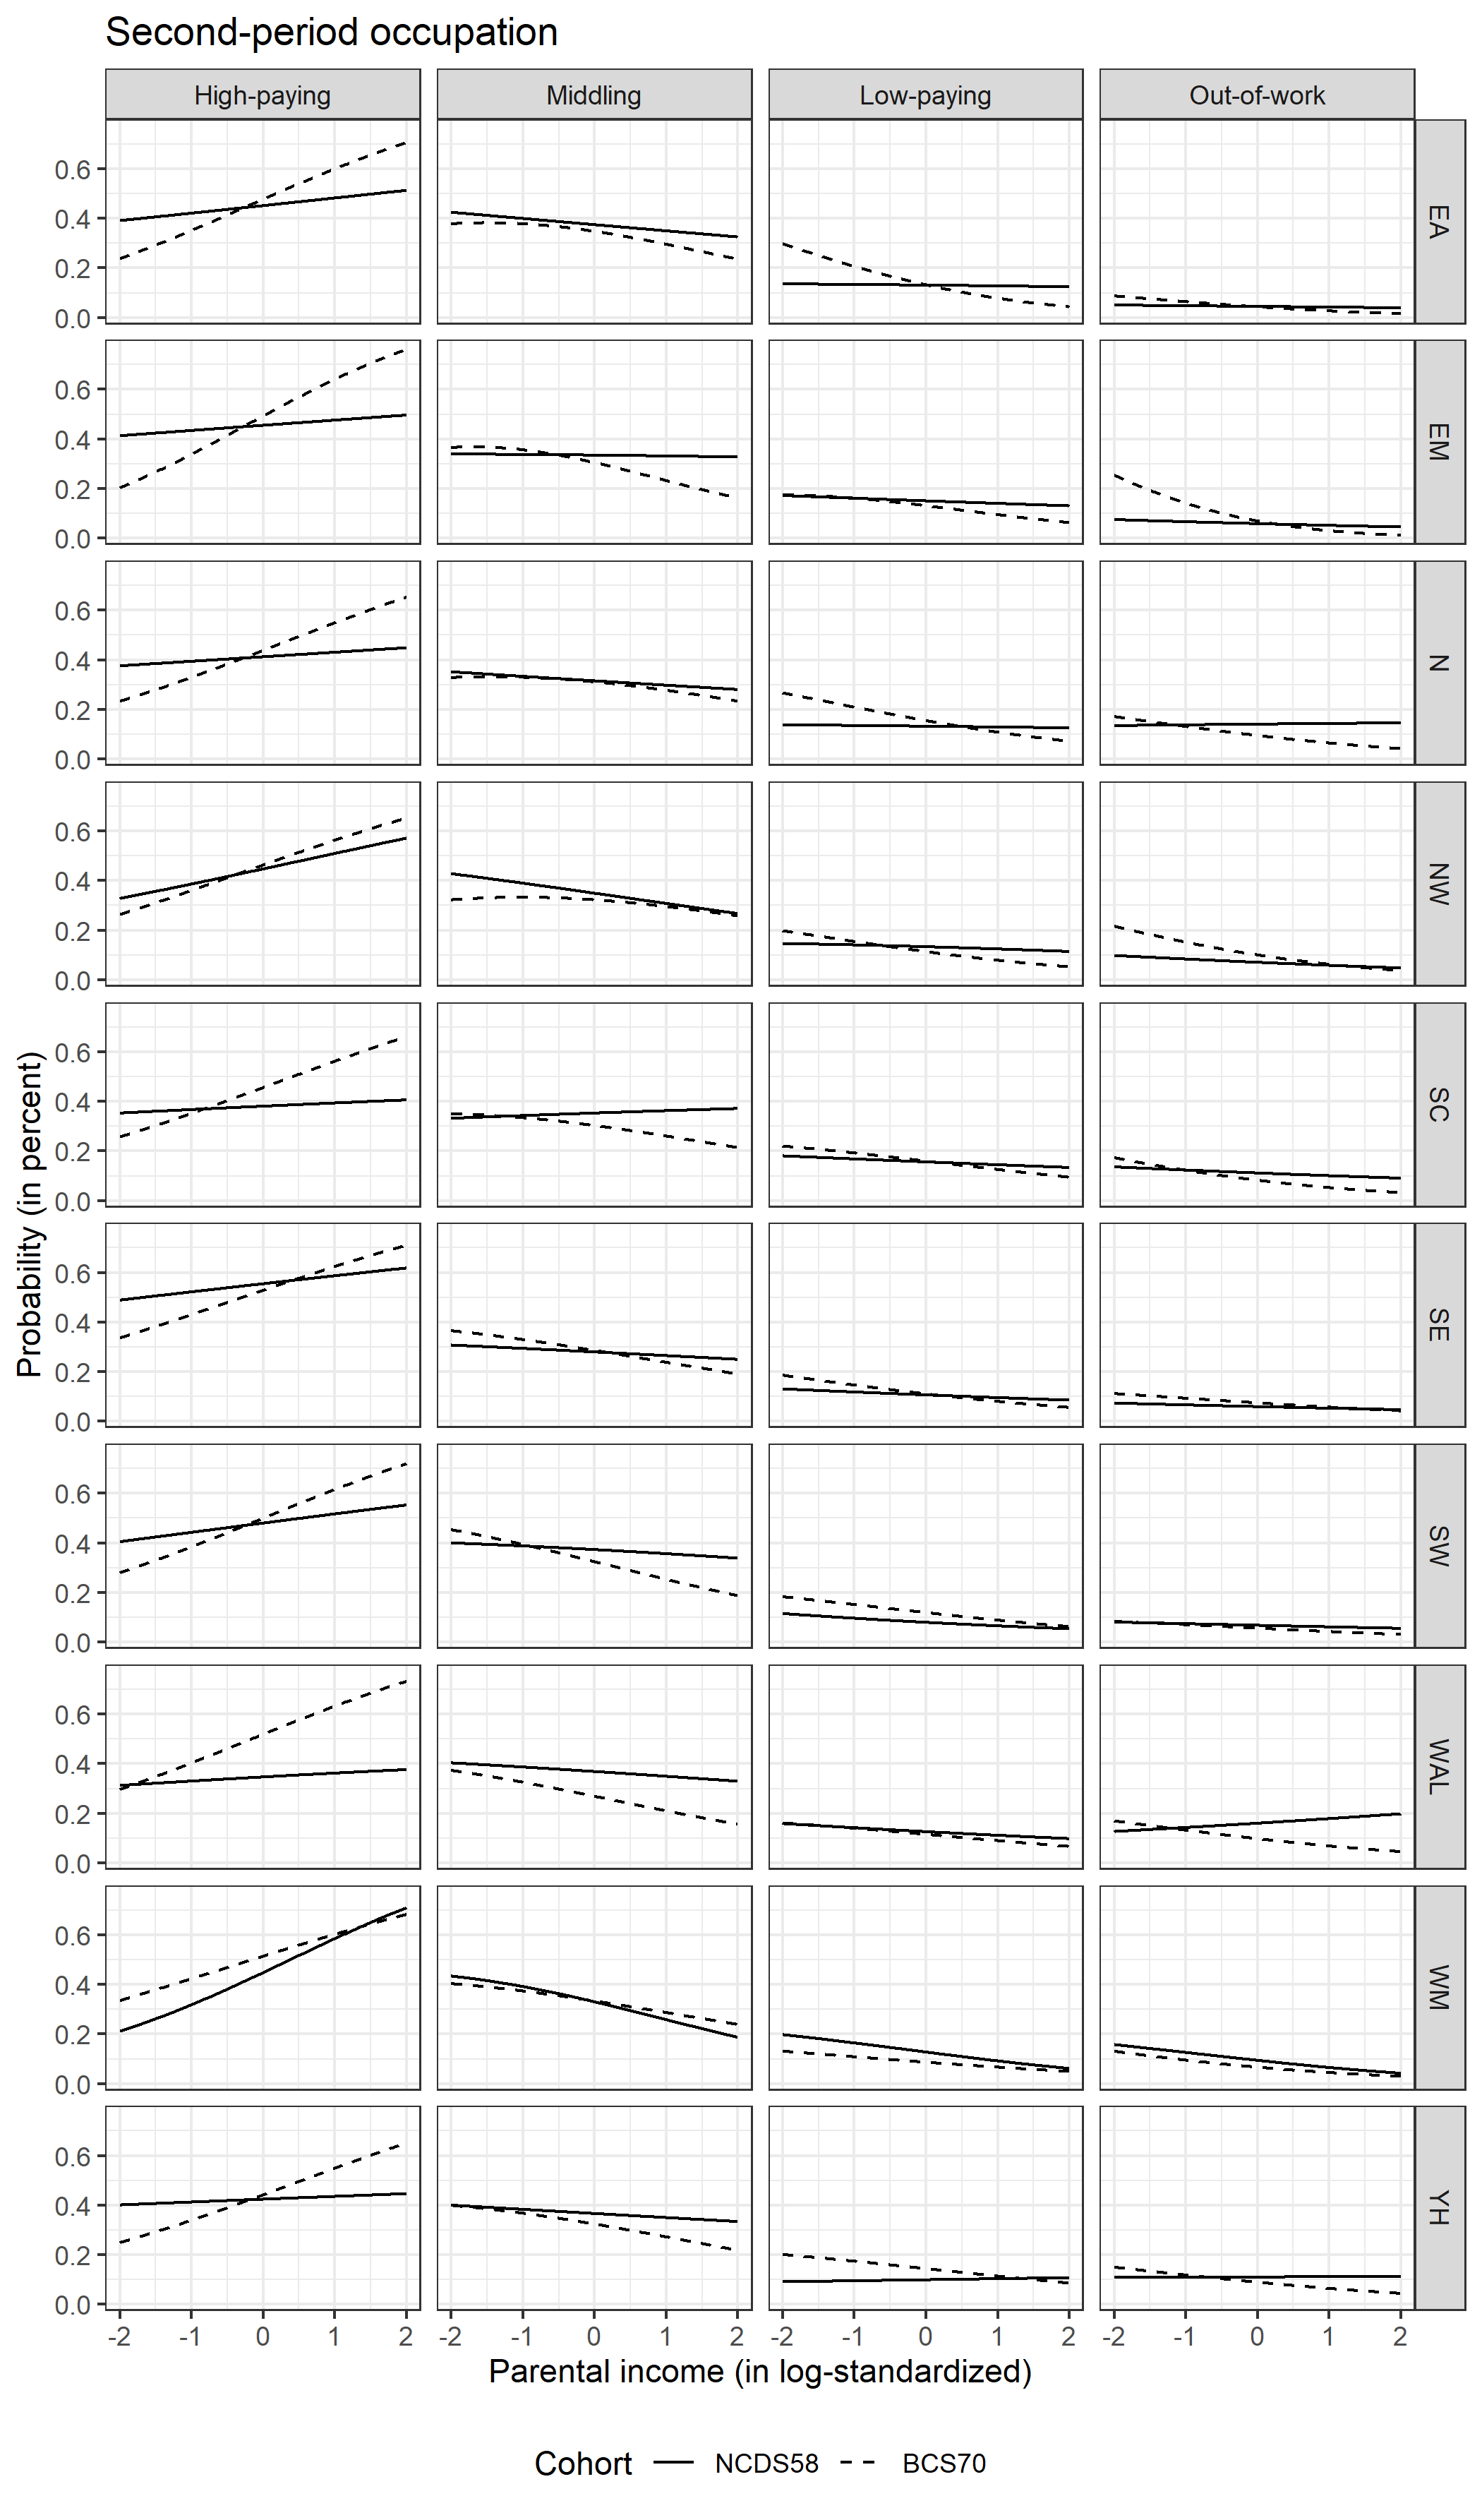
\includegraphics[width=.7\linewidth]{chap2/graphic/reg-multi2-pinc-male.png}
    \vspace{-3em}
	\justify\singlespacing\footnotesize{\textit{Notes:} This figure presents the probability, expressed in percent, of being in each type of occupation (out-of-work, low-paying, middling, high-paying) in second period according to parental income, in log-standardized, for each region.
	Probabilities are computed for males in both cohorts according to the multinomial logistic regressions reported in Table \ref{chap2-tab:reg-multi2-short}.}
\end{figure}

\begin{figure}[!htb]
    \centering
    \caption{Second-period occupation probability according to parental income at the regional level (female only)}
    \label{chap2-fig:reg-multi2-pinc-female}
    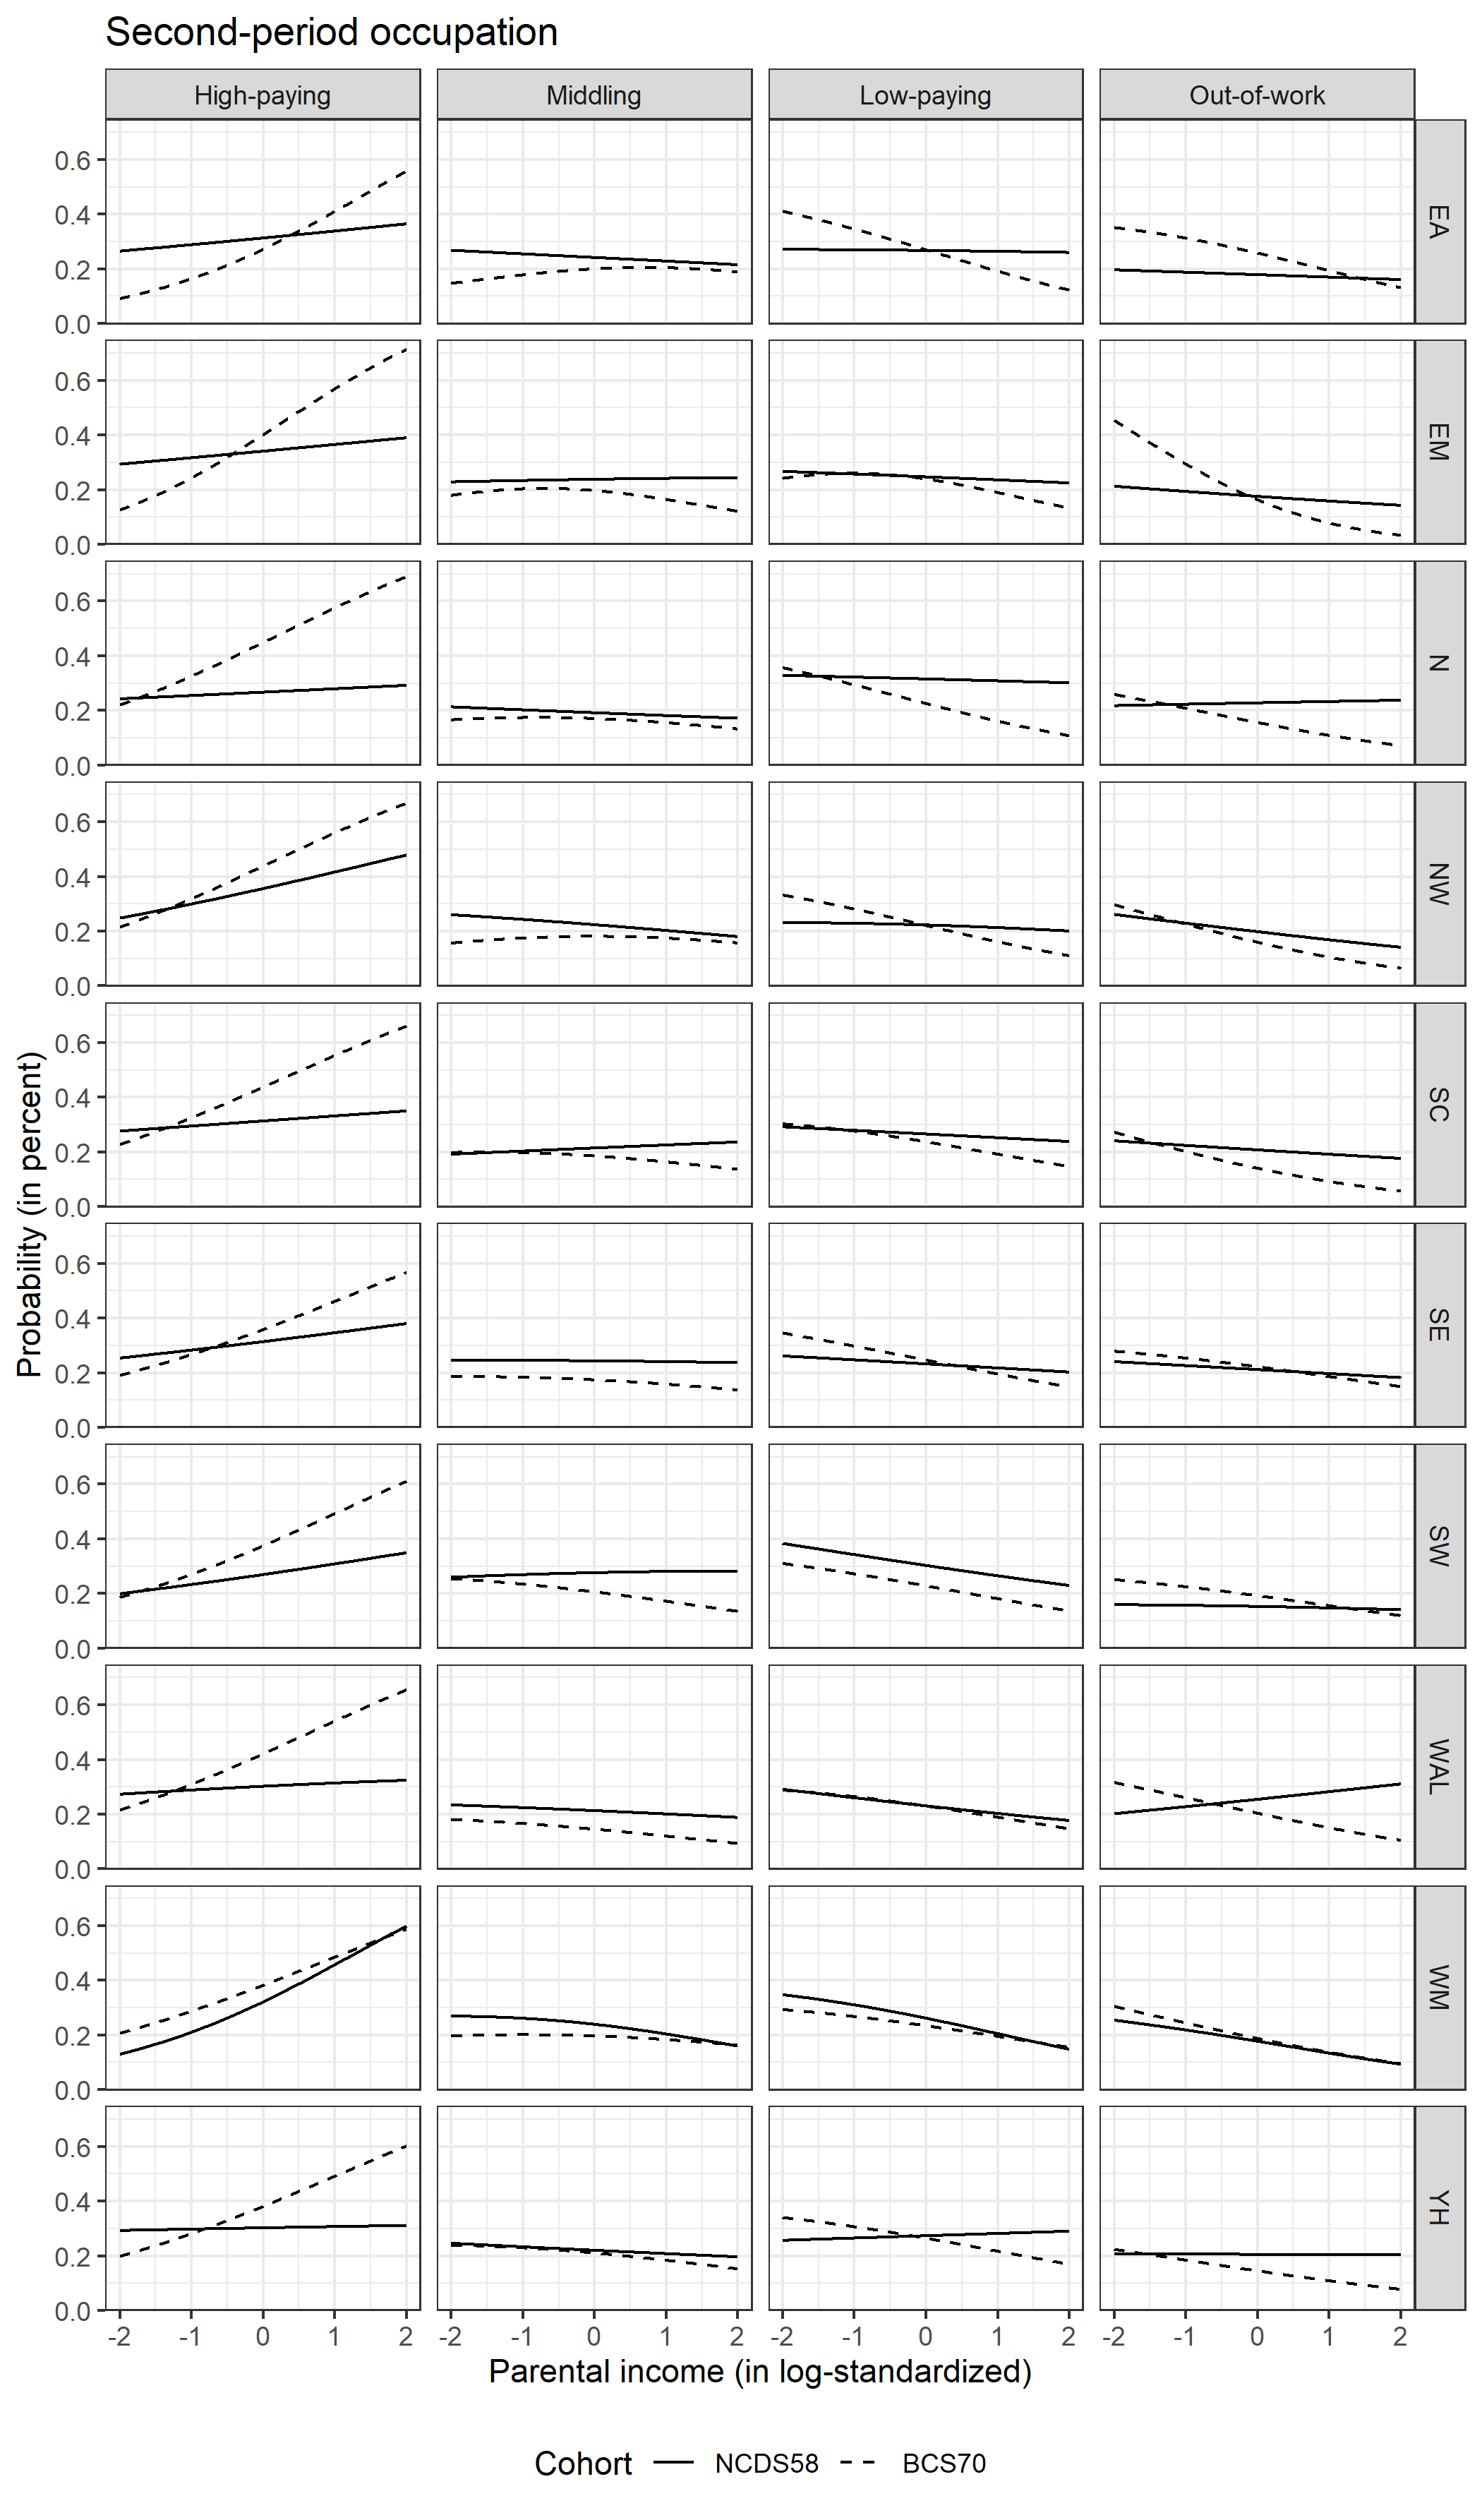
\includegraphics[width=.7\linewidth]{chap2/graphic/reg-multi2-pinc-female.png}
    \vspace{-3em}
	\justify\singlespacing\footnotesize{\textit{Notes:} This figure presents the probability, expressed in percent, of being in each type of occupation (out-of-work, low-paying, middling, high-paying) in second period according to parental income, in log-standardized, for each region.
	Probabilities are computed for females in both cohorts according to the multinomial logistic regressions reported in Table \ref{chap2-tab:reg-multi2-short}.}
\end{figure}

\begin{landscape}
\begin{table}[!tb]
    \centering
    \caption{Probability of being in each occupation in the second period according to the shares of middling and high-paying occupations in the region at the age 16 (multinomial)}
    \label{chap2-tab:regocc-multi2B-short}
    % \resizebox*{!}{\dimexpr\textheight-2\baselineskip\relax}{
    % \resizebox*{\textwidth}{!}{
    \begin{threeparttable}
        \setlength{\tabcolsep}{-1pt}
        \begin{tabular}{l D{.}{.}{5.3} D{.}{.}{5.5} D{.}{.}{5.5} D{.}{.}{5.3} D{.}{.}{5.5} D{.}{.}{5.5} D{.}{.}{5.3} D{.}{.}{5.5} D{.}{.}{5.5}}
\toprule
 & \multicolumn{9}{c}{Multinomial logit - Dep. var.: Second-period occupation} \\
\cmidrule(lr){2-10}
 & \multicolumn{3}{c}{(1)} & \multicolumn{3}{c}{(2)} & \multicolumn{3}{c}{(3)} \\
\cmidrule(lr){2-4}\cmidrule(lr){5-7}\cmidrule(lr){8-10}
 & \multicolumn{1}{c}{Low} & \multicolumn{1}{c}{Mid} & \multicolumn{1}{c}{High} & \multicolumn{1}{c}{Low} & \multicolumn{1}{c}{Mid} & \multicolumn{1}{c}{High} & \multicolumn{1}{c}{Low} & \multicolumn{1}{c}{Mid} & \multicolumn{1}{c}{High} \\
\midrule
Middling share                 & -0.07  & -0.02      & -0.17^{***} &        &            &            & 0.22   & -0.22      & -0.21       \\
                               & (0.06) & (0.05)     & (0.05)      &        &            &            & (0.34) & (0.32)     & (0.30)      \\
High-paying share              &        &            &             & 0.10   & -0.01      & 0.28^{***} & 0.37   & -0.41      & -0.25       \\
                               &        &            &             & (0.07) & (0.06)     & (0.06)     & (0.51) & (0.48)     & (0.46)      \\
Parental income                & 0.04   & 0.11^{***} & 0.35^{***}  & 0.04   & 0.11^{***} & 0.36^{***} & 0.05   & 0.12^{***} & 0.38^{***}  \\
                               & (0.03) & (0.03)     & (0.03)      & (0.03) & (0.03)     & (0.03)     & (0.03) & (0.03)     & (0.03)      \\
Par. inc. $\times$ Mid. share  & 0.00   & -0.04^{*}  & -0.11^{***} &        &            &            & -0.06  & -0.13^{**} & -0.29^{***} \\
                               & (0.03) & (0.02)     & (0.02)      &        &            &            & (0.06) & (0.05)     & (0.05)      \\
Par. inc. $\times$ High. share &        &            &             & -0.01  & 0.02       & 0.05^{**}  & -0.06  & -0.09^{*}  & -0.17^{***} \\
                               &        &            &             & (0.02) & (0.02)     & (0.02)     & (0.05) & (0.05)     & (0.05)      \\
\midrule
Num. obs. & \multicolumn{1}{c}{14763} & \multicolumn{1}{c}{14763} & \multicolumn{1}{c}{14763} & \multicolumn{1}{c}{14763} & \multicolumn{1}{c}{14763} & \multicolumn{1}{c}{14763} & \multicolumn{1}{c}{14763} & \multicolumn{1}{c}{14763} & \multicolumn{1}{c}{14763}\\
\bottomrule
\end{tabular}

        \begin{tablenotes}[flushleft]
            \footnotesize{\item\textit{Notes}: 
            % Stars and SE
            $^{***}p<0.01$; $^{**}p<0.05$; $^{*}p<0.1$. Standard errors between parentheses. 
            % Baseline outcome
            Out-of-work occupation in second period is the base outcome of the multinomial logistic regression.
            % Referent group
            Male is the referent group in all regressions.
            % Variables details
            Parental income in logarithm and then standardized at the cohort level. Middling and High-paying shares correspond to, respectively, the shares of middling and high-paying in total employment in the region at age 16. Both shares have been standardized for the interpretability of coefficients when interacted with parental income.
            % Control variables
            Control variables in (1) include Intercept, Female and Female $\times$ BCS, while control variables in (2) include Intercept, Female and Female $\times$ Non-Mid. share. %; see Table \ref{chap2-tab:tobefilled} in the appendix for these coefficients.
            }
        \end{tablenotes}
    \end{threeparttable}
    % }}
\end{table}
\end{landscape}

\begin{figure}[!tb]
    \centering
    \caption{Change in parental income coefficient for second-period occupation according to job polarization at the regional level}
    \label{chap2-fig:regocc-absolute-all}
    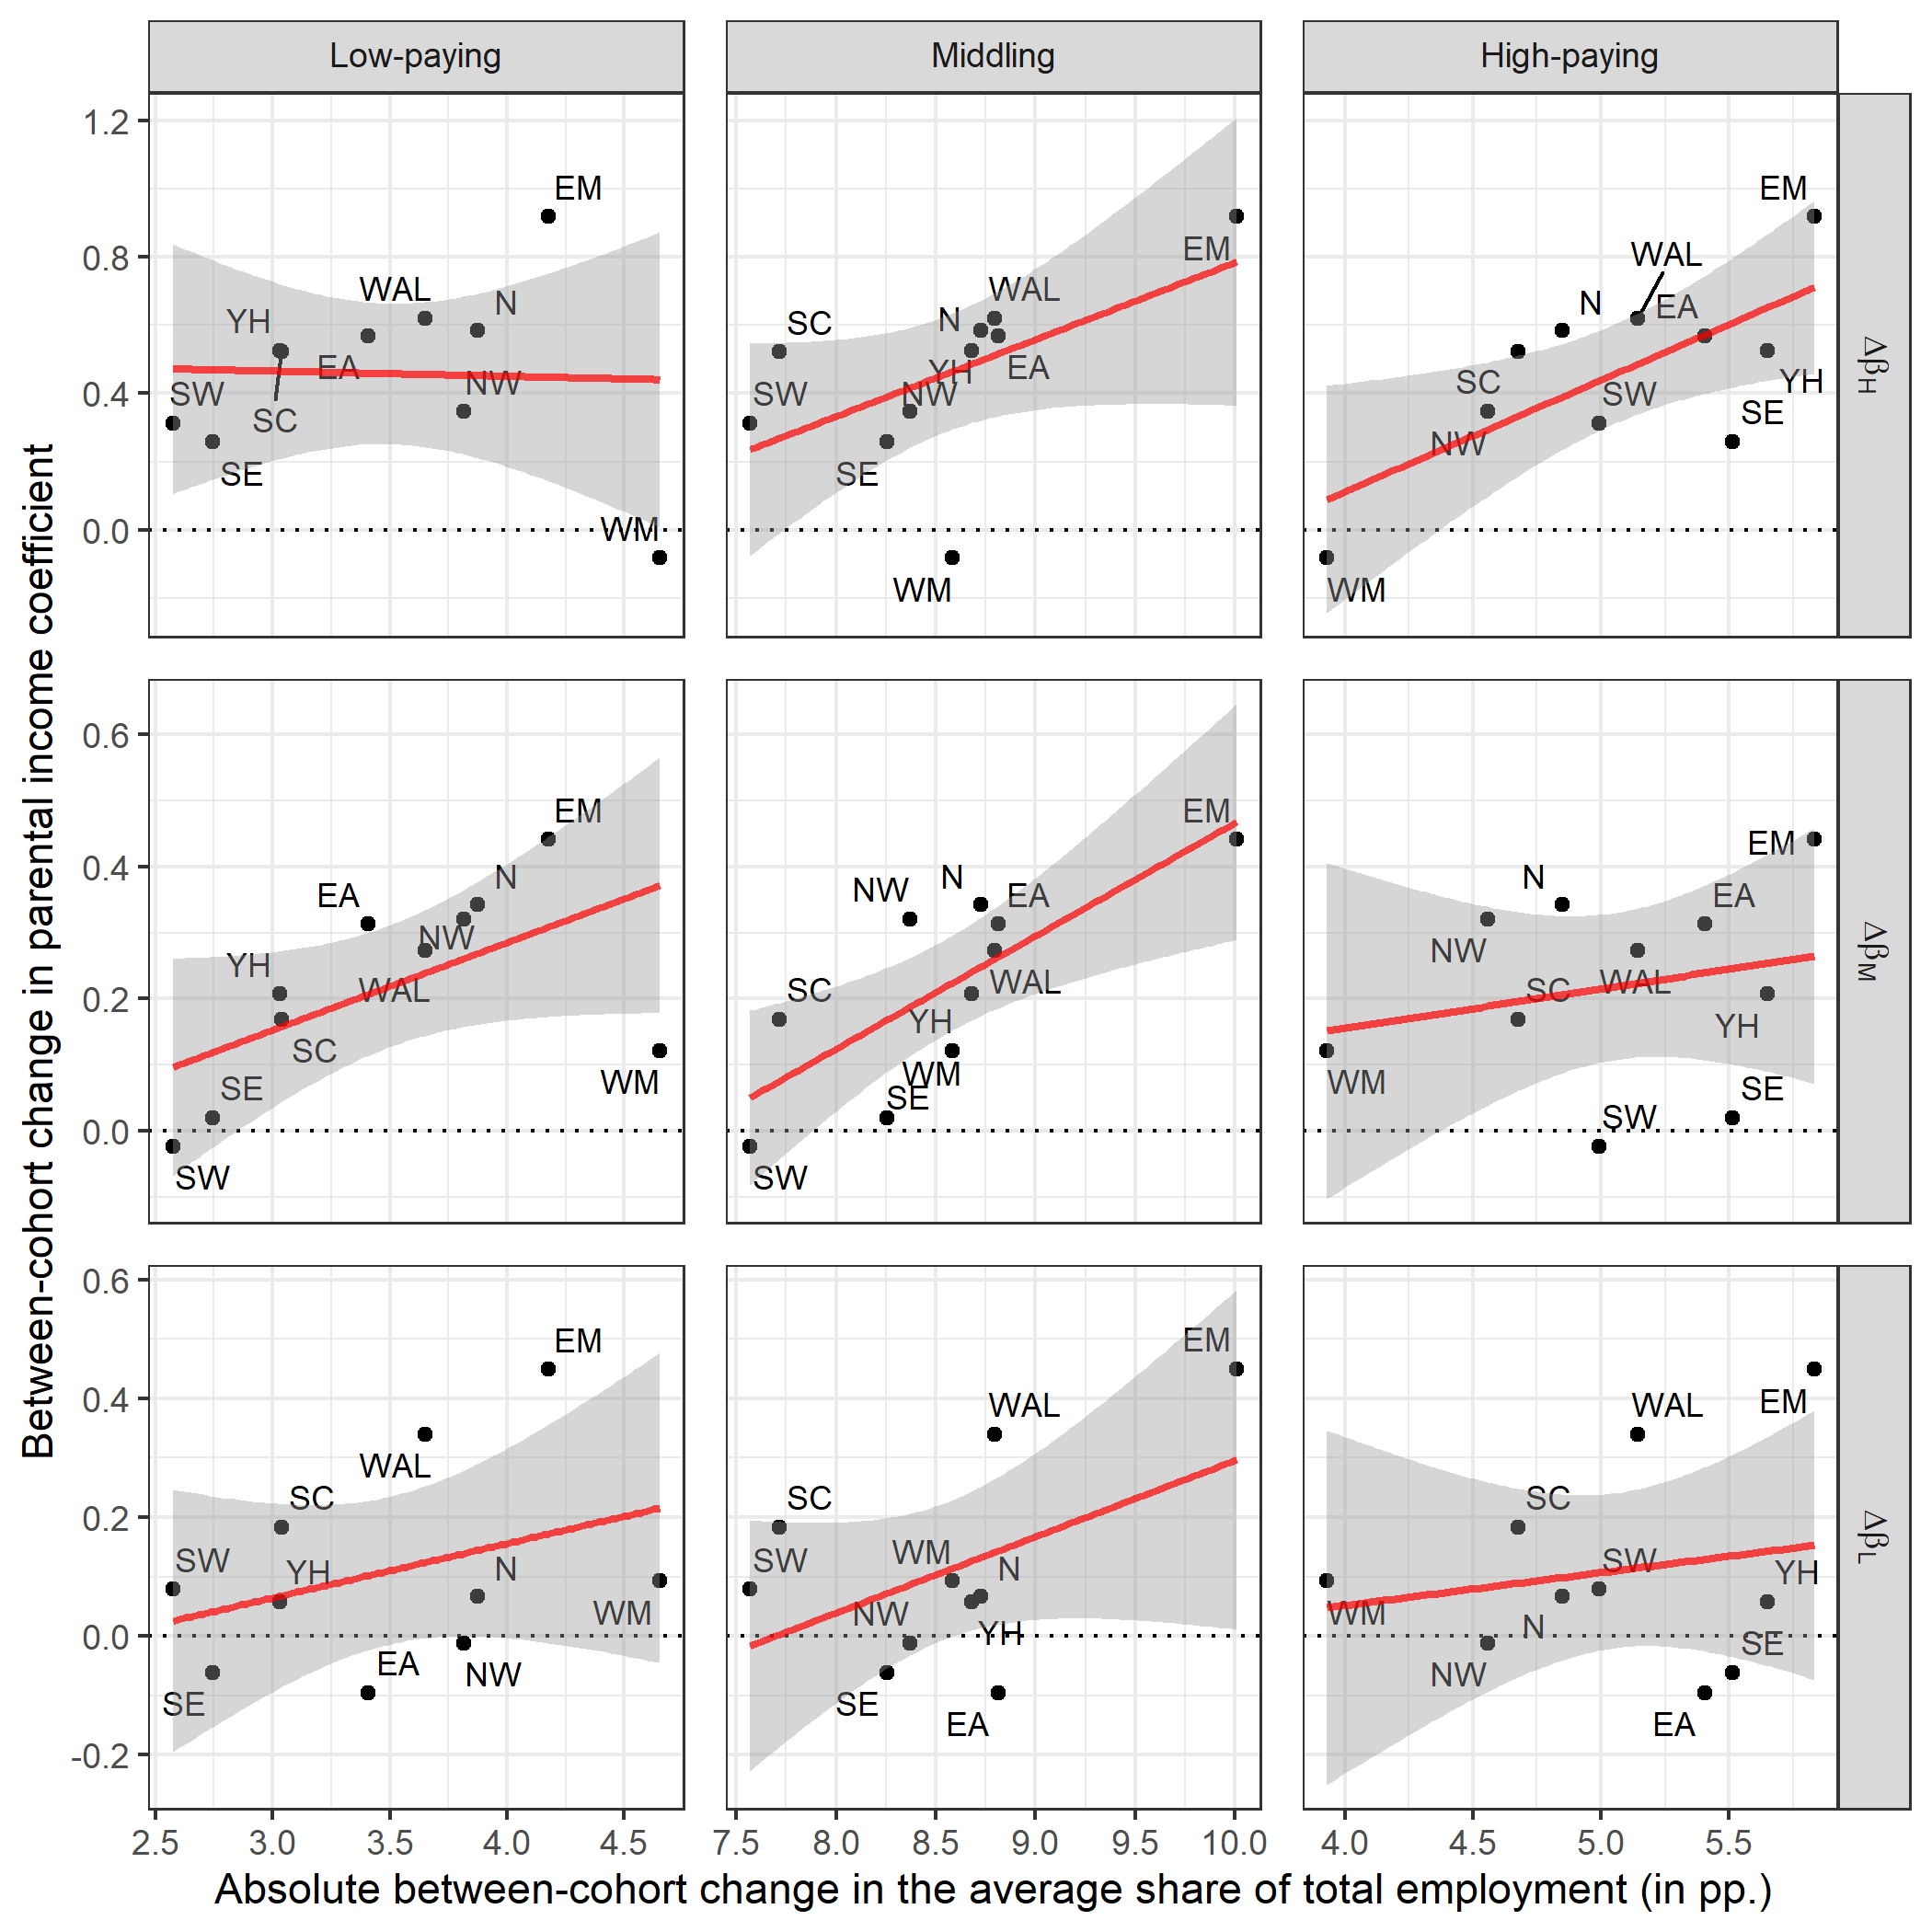
\includegraphics[width=\linewidth]{chap2/graphic/regocc-absolute-all.png}
    \vspace{-3em}
	\justify\singlespacing\footnotesize{\textit{Notes:} This figure presents the correlation across regions between the change in the parental income coefficient for each occupation (low-paying, middling, and high-paying) in second period $\Delta\beta_k$ and the between-cohort change in absolute value in the average share of total employment of low-paying, middling, and high-paying occupations, in percentage points. Note that, by taking the absolute value of the change, we reversed the x-axis for the middling panels (middle column). Thus, regions on the left-hand (resp. right-hand) side of each panel are those where the polarization of employment has been lower (resp. larger).}
\end{figure}
    \clearpage
    \subsection{Decomposing the effect of parental income}\label{chap2-app-decomposing}
    %\subsubsection{Decomposing the effect of parental income} \label{chap2-trade-off}

This appendix examines how the effect of parental income on the occupations of mature workers operates through its impact on both first and second period occupations. Our results indicate that, conditional on first period occupation, the role of parental income in determining occupational outcomes has increased. At the same time, as is clear from the regressions, initial occupations are also important to determine outcomes at age 42. In particular, those who started their careers in middling have a probability to move to high-paying occupations that is about 7 pp. higher than those who started in a low-paying occupation (see Table \ref{chap2-tab:proba-group5-cdt-short}). Similarly, entering the labour market in a middling occupation implies a likelihood to be in such an occupation at age 42 at least 20 pp. higher than entering in a low-paying job. We would hence like to assess to what extent parental income compensates for past occupations. 

We compare the probability to be in a middling occupation at age 42 for two individuals who started in different initial occupations, middling and low-paying, and compute the additional parental income that the latter would need to have in order to compensate the advantage given by starting work in a middling occupation. To do so, we define the ratio between the two probabilities
\begin{equation}\label{chap2-eq:relative-proba}
    \frac{p_{M}^{M}}{p_{M}^{L}} = \frac{p_O^M}{p_O^L}\exp\Big(\eta_{MM} -\eta_{ML} + \beta_{3M} (Y^M-Y^L)\Big),
\end{equation}
where $p^j_k$ is the probability of being in occupation $k$ in second period conditional on having started in occupation $j$, and $Y^L$ and $Y^M$ are, respectively, the parental income of the individual starting in a low-paying occupation and of that starting in a middling occupation. 

For both cohorts, we derive the parental income $Y^c=Y^L-Y^M$ such that the two individuals are as likely to be in a middling occupation at age 42, i.e. $p_{M}^{M}=p_{M}^{L}$. Thus,
\begin{equation}\label{chap2-eq:counter-Y}
    Y^c \equiv \frac{\eta^c}{\beta^c} = \frac{\eta^c_{MM} -\eta^c_{ML} - \log(p_O^M/p_O^L)}{\beta^c_{3M}},
\end{equation}
where $p_O^M$ and $p_O^L$ are evaluated at the mean of the parental income distribution. We interpret $Y^c$ as the additional parental income that an individual in cohort $c$ starting in occupation $L$ needs in order to be as likely as one starting in occupation $M$ to be in a middling occupation when mature.
Thus, $\eta^c$ captures the degree of persistence in $M$, whereas $\beta^c$ reflects the effectiveness of parental income in moving into a middling occupation in second period. The greater the degree of persistence in $M$, the greater the parental income required to compensate the advantage given by the first-period occupation, i.e. $\partial Y^c/\partial\eta^c > 0$. The greater the effectiveness of parental income, the smaller the parental income required to compensate, i.e. $\partial Y^c/\partial\beta^c < 0~\forall\Delta\beta > 0$.

This difference in parental income reflects the value conferred by being in a certain first-period occupation---compared to parental income---for mobility across occupations. Taking the ratio between $Y^{70}$ and $Y^{58}$, we obtain the \emph{change across cohorts in the relative advantage} such that
\begin{equation}\label{chap2-eq:delta-Y}
    \Delta Y \equiv \frac{Y^{70}}{Y^{58}}= \frac{\Delta\eta}{\Delta\beta}
\end{equation}
where $\Delta\eta = \eta^{70}/\eta^{58}$ captures the effect of the change in the degree of persistence and $\Delta\beta = \beta^{70}/\beta^{58}$ reflects the effect of the change in the role of parental income. 
Both affect the worth of the first-period occupation in opposite ways.
%\footnote{ 
The greater the change in the degree of persistence, the greater the change in parental income needed to compensate, hence, the greater the relative worth of first-period occupation, i.e. $\partial\Delta Y/\partial\Delta\eta > 0$.
The greater the change in the effectiveness of parental income, the smaller the change in the parental income to compensate, hence, the smaller the relative worth of first-period occupation, i.e. $\partial\Delta Y/\partial\Delta\beta < 0~\forall\Delta\beta > 0$.
%}

Table \ref{chap2-tab:decomp-all} presents the decomposition of the relative advantage of first-period occupation---compared to parental income---for upward mobility.
\begin{table}[!tb]
    \centering
    \caption{Relative advantage of the first-period occupation with respect to parental income}
    \label{chap2-tab:decomp-all}
    \begin{threeparttable}
        \setlength{\tabcolsep}{9pt}
        
\begin{tabular}{lrrrrrrrrr}
\toprule
\multicolumn{1}{c}{} & \multicolumn{3}{c}{$p_{M}^{M}=p_{M}^{L}$} & \multicolumn{3}{c}{$p_{H}^{H}=p_{H}^{M}$} & \multicolumn{3}{c}{$p_{H}^{H}=p_{H}^{L}$} \\
\cmidrule(l{3pt}r{3pt}){2-4} \cmidrule(l{3pt}r{3pt}){5-7} \cmidrule(l{3pt}r{3pt}){8-10}
  & \multicolumn{1}{c}{$Y$} & \multicolumn{1}{c}{$\eta$} & \multicolumn{1}{c}{$\beta$} & \multicolumn{1}{c}{$Y$} & \multicolumn{1}{c}{$\eta$} & \multicolumn{1}{c}{$\beta$} & \multicolumn{1}{c}{$Y$} & \multicolumn{1}{c}{$\eta$} & \multicolumn{1}{c}{$\beta$}\\
\midrule
BCS70 & 4.63 & 0.73 & 0.16 & 2.13 & 0.84 & 0.39 & 2.25 & 0.89 & 0.39\\
NCDS58 & 13.11 & 0.60 & 0.05 & 5.47 & 0.79 & 0.14 & 6.24 & 0.90 & 0.14\\
\midrule
$\Delta$ & 0.35 & 1.22 & 3.45 & 0.39 & 1.07 & 2.74 & 0.36 & 0.99 & 2.74\\
\midrule
$\Delta$ ($\eta$ constant) & 0.29 & 1.00 & 3.45 & 0.37 & 1.00 & 2.74 & 0.37 & 1.00 & 2.74\\
$\Delta$ ($\beta$ constant) & 1.22 & 1.22 & 1.00 & 1.07 & 1.07 & 1.00 & 0.99 & 0.99 & 1.00\\
\bottomrule
\end{tabular}

        \begin{tablenotes}[flushleft]
            \footnotesize{\item\textit{Notes}: This table presents the relative advantage of the first-period occupation with respect to parental income for upward mobility. 
            $Y$ corresponds to the parental income that an individual in cohort $c$ needs in order to compensate for having started one occupational category below, $\eta$ captures the degree of persistence, whereas $\beta$ captures the effectiveness of parental income. 
            Coefficients for the NCDS58 and BCS70 cohorts are computed for males using Table \ref{chap2-tab:occ-multi23-base} in the appendix.
            $\Delta$ rows refer to the ratio between the BCS70 and NCDS58 under three specifications: the actual ratio, the ratio keeping $\eta$ constant, and the ratio keeping $\beta$ constant.}
        \end{tablenotes}
    \end{threeparttable}
\end{table}
We consider three cases: the difference in reaching a middling occupation for those starting in low-paying or in middling occupations (left panel), the difference in reaching a high-paying occupation for those starting in high-paying or in middling occupations (middle panel), and the difference in reaching a high-paying occupation for those starting in low-paying or in high-paying occupations (right panel). 

% BUT recall that parental income was ABSOLUTELY less important to determine first-period occ. in the NCDS58. Also eta has increased so the ABSOLUTE value of initial occupation has increased 

Consider first the relative effect of initial occupations versus parental income for the NCDS58. Because parental income is standardized, the figures reported for $Y^{70}$ represent the standard deviations needed to compensate the difference when starting in the various initial occupations (computed at the mean of parental income.). For the three cases we report, the additional income required is between 5.47 and 13.11 standard deviations. Such large magnitudes imply that it was hard for parental income to compensate the advantage conferred by a more favourable initial occupation, and, in the case of the probabilities of being in a middling occupation at age 42 ($p_M^M$  and $p_M^L$, left panel) only a massive difference in parental income could compensate the advantage that being in a middling occupation at 23 conferred. When we compare these figures with those for the BCS70, we can see that the additional income required to compensate the most favourable occupation is between 2.13 and 4.63 standard deviations, magnitudes that amount to about a third of those needed for the older cohort. 

The bottom two lines allow us to understand what is driving this change. We compute the ratio $Y^{70}/Y^{58}$ by keeping constant, i.e. at the value it had for the NCDS58, either $\eta$ or $\beta$. Recall from equation (5) that $\eta$ captures the degree of persistence in an occupation, whereas $\beta$ reflects the advantage to move upwards conferred by parental income. The three cases we examine display the same pattern. When we keep $\eta$ constant we obtain a change in the relative importance of parental income that is very close to the actual one, indicating that changes in persistence have played a minor role. In contrast, keeping $\beta$ constant results in values of $\Delta Y$ that are around or above 1. That is, what is driving the differences across cohorts in the advantage that parental income affords relative to initial occupations is the direct effect of the former rather than any changes in persistence associated with the latter.

These results indicate that there has been a major change in the relative roles that entry jobs and parental background play in determining the occupational outcomes of mature individuals. For the older cohort, the advantage conferred by entry occupations could only be offset by vast amounts of parental income; for the younger one, the latter has become much more able to offset the career advantages conferred by early career experiences.

    \clearpage
    \subsection{Robustness checks}\label{chap2-app-robustness}
    \subsubsection{Squared parental income}

This appendix provides a robustness check on the role of squared parental income. We consider the non-logarithmic parental income although standardized.
Table \ref{chap2-tab:rob1-multi1-base} shows the coefficients of the multinomial logistic regression for the probability of being in each first-period occupation.
Table \ref{chap2-tab:rob1-multi2-base} shows the coefficients of the multinomial logistic regression for the probability of being in each second-period occupation.
Table \ref{chap2-tab:rob1-multi3-base} shows the coefficients of the multinomial logistic regression for the probability of being in each second-period occupation according to first-period occupation.

\begin{table}[!htb]
    \centering
    \caption{Probability of being in each occupation in first period (Squared-parental-income robustness check)}
    \label{chap2-tab:rob1-multi1-base}
    \resizebox{\textwidth}{!}{
    \begin{threeparttable}
        \setlength{\tabcolsep}{0pt}
        \begin{tabular}{l D{.}{.}{5.5} D{.}{.}{5.5} D{.}{.}{5.5} D{.}{.}{5.5} D{.}{.}{5.5} D{.}{.}{5.5}}
\toprule
 & \multicolumn{6}{c}{Multinomial logit - Dep. var.: First-period occupation} \\
\cmidrule(lr){2-7}
 & \multicolumn{3}{c}{(1)} & \multicolumn{3}{c}{(2)} \\
\cmidrule(lr){2-4}\cmidrule(lr){5-7}
 & \multicolumn{1}{c}{Low} & \multicolumn{1}{c}{Mid} & \multicolumn{1}{c}{High} & \multicolumn{1}{c}{Low} & \multicolumn{1}{c}{Mid} & \multicolumn{1}{c}{High} \\
\midrule
Intercept                  & 0.08        & 1.39^{***}  & 0.69^{***}  & 0.06        & 1.38^{***}  & 0.66^{***}  \\
                           & (0.07)      & (0.06)      & (0.06)      & (0.07)      & (0.06)      & (0.06)      \\
BCS cohort                 & 0.23^{**}   & 0.12        & 0.76^{***}  & 0.29^{***}  & 0.25^{***}  & 0.90^{***}  \\
                           & (0.10)      & (0.08)      & (0.09)      & (0.11)      & (0.09)      & (0.09)      \\
Female                     & -0.79^{***} & -1.27^{***} & -1.00^{***} & -0.79^{***} & -1.27^{***} & -1.00^{***} \\
                           & (0.09)      & (0.07)      & (0.08)      & (0.09)      & (0.07)      & (0.08)      \\
Female $\times$ BCS        & 0.25^{**}   & -0.01       & -0.07       & 0.25^{**}   & -0.02       & -0.07       \\
                           & (0.12)      & (0.10)      & (0.11)      & (0.12)      & (0.10)      & (0.11)      \\
Par. inc.                  & -0.03       & 0.02        & 0.28^{***}  & -0.04       & 0.02        & 0.26^{***}  \\
                           & (0.04)      & (0.03)      & (0.04)      & (0.04)      & (0.03)      & (0.04)      \\
Par. inc. $\times$ BCS     & 0.09        & 0.20^{***}  & 0.35^{***}  & 0.11        & 0.28^{***}  & 0.46^{***}  \\
                           & (0.06)      & (0.05)      & (0.05)      & (0.07)      & (0.06)      & (0.06)      \\
Par. inc.$^2$              &             &             &             & 0.02        & 0.01        & 0.03        \\
                           &             &             &             & (0.03)      & (0.02)      & (0.02)      \\
Par. inc.$^2$ $\times$ BCS &             &             &             & -0.06       & -0.14^{***} & -0.15^{***} \\
                           &             &             &             & (0.04)      & (0.03)      & (0.03)      \\
\midrule
Num. obs. & \multicolumn{1}{c}{14763} & \multicolumn{1}{c}{14763} & \multicolumn{1}{c}{14763} & \multicolumn{1}{c}{14763} & \multicolumn{1}{c}{14763} & \multicolumn{1}{c}{14763}\\
\bottomrule
\end{tabular}

        \begin{tablenotes}[flushleft]
            \footnotesize{\item\textit{Notes}:
            % Stars and SE
            $^{***}p<0.01$; $^{**}p<0.05$; $^{*}p<0.1$. Standard errors between parentheses. 
            % Referent group
            Male in the NCDS58 cohort is the referent group. 
            % Variables details
            Parental income is standardized at the cohort level and squared parental-income is the square of the standardized parental income.}
        \end{tablenotes}
    \end{threeparttable}
    }
\end{table}

\begin{table}[!htb]
    \centering
    \caption{Probability of being in each occupation in second period (Squared-parental-income robustness check)}
    \label{chap2-tab:rob1-multi2-base}
    \resizebox{\textwidth}{!}{
    \begin{threeparttable}
        \setlength{\tabcolsep}{0pt}
        \begin{tabular}{l D{.}{.}{5.5} D{.}{.}{5.5} D{.}{.}{5.5} D{.}{.}{5.5} D{.}{.}{5.5} D{.}{.}{5.5}}
\toprule
 & \multicolumn{6}{c}{Multinomial logit - Dep. var.: Second-period occupation} \\
\cmidrule(lr){2-7}
 & \multicolumn{3}{c}{(1)} & \multicolumn{3}{c}{(2)} \\
\cmidrule(lr){2-4}\cmidrule(lr){5-7}
 & \multicolumn{1}{c}{Low} & \multicolumn{1}{c}{Mid} & \multicolumn{1}{c}{High} & \multicolumn{1}{c}{Low} & \multicolumn{1}{c}{Mid} & \multicolumn{1}{c}{High} \\
\midrule
Intercept                  & 0.37^{***} & 1.37^{***}  & 1.69^{***}  & 0.45^{***}  & 1.46^{***}  & 1.72^{***}  \\
                           & (0.08)     & (0.07)      & (0.07)      & (0.08)      & (0.07)      & (0.07)      \\
BCS cohort                 & 0.03       & -0.05       & 0.11        & 0.06        & 0.03        & 0.22^{**}   \\
                           & (0.11)     & (0.09)      & (0.09)      & (0.12)      & (0.10)      & (0.10)      \\
Female                     & -0.13      & -1.22^{***} & -1.24^{***} & -0.12       & -1.22^{***} & -1.24^{***} \\
                           & (0.09)     & (0.08)      & (0.08)      & (0.09)      & (0.08)      & (0.08)      \\
Female $\times$ BCS        & -0.04      & -0.12       & 0.17        & -0.05       & -0.13       & 0.17        \\
                           & (0.13)     & (0.12)      & (0.11)      & (0.13)      & (0.12)      & (0.11)      \\
Par. inc.                  & -0.02      & 0.02        & 0.25^{***}  & -0.01       & 0.03        & 0.25^{***}  \\
                           & (0.04)     & (0.04)      & (0.04)      & (0.04)      & (0.04)      & (0.04)      \\
Par. inc. $\times$ BCS     & 0.03       & 0.12^{**}   & 0.28^{***}  & 0.09        & 0.22^{***}  & 0.39^{***}  \\
                           & (0.06)     & (0.06)      & (0.06)      & (0.07)      & (0.06)      & (0.06)      \\
Par. inc.$^2$              &            &             &             & -0.08^{***} & -0.09^{***} & -0.02       \\
                           &            &             &             & (0.03)      & (0.03)      & (0.02)      \\
Par. inc.$^2$ $\times$ BCS &            &             &             & -0.02       & -0.07^{*}   & -0.11^{***} \\
                           &            &             &             & (0.04)      & (0.04)      & (0.03)      \\
\midrule
Num. obs. & \multicolumn{1}{c}{14763} & \multicolumn{1}{c}{14763} & \multicolumn{1}{c}{14763} & \multicolumn{1}{c}{14763} & \multicolumn{1}{c}{14763} & \multicolumn{1}{c}{14763}\\
\bottomrule
\end{tabular}

        \begin{tablenotes}[flushleft]
            \footnotesize{\item\textit{Notes}: 
            % Stars and SE
            $^{***}p<0.01$; $^{**}p<0.05$; $^{*}p<0.1$. Standard errors between parentheses. 
            % Referent group
            Male in the NCDS58 cohort in out-of-work occupation in first period is the referent group. 
            % Variables details
            Parental income is standardized at the cohort level and squared parental-income is the square of the standardized parental income.
            % Explaining bottom panels
            Coefficients in the first bottom panel captures the change in the marginal effect of the first-period occupation with respect to the referent one, i.e. out-of-work. 
            Coefficients in the second bottom panel indicates the change across cohorts in the marginal effect of the first-period occupation.}
        \end{tablenotes}
    \end{threeparttable}
    }
\end{table}

\begin{table}[!htb]
    \centering
    \caption{Probability of being in each occupation in second period (Squared-parental-income robustness check)}
    \label{chap2-tab:rob1-multi3-base}
    \resizebox{\textwidth}{!}{
    \begin{threeparttable}
        \setlength{\tabcolsep}{0pt}
        \begin{tabular}{l D{.}{.}{5.5} D{.}{.}{5.5} D{.}{.}{5.5} D{.}{.}{5.5} D{.}{.}{5.5} D{.}{.}{5.5}}
\toprule
 & \multicolumn{6}{c}{Multinomial logit - Dep. var.: Second-period occupation} \\
\cmidrule(lr){2-7}
 & \multicolumn{3}{c}{(1)} & \multicolumn{3}{c}{(2)} \\
\cmidrule(lr){2-4}\cmidrule(lr){5-7}
 & \multicolumn{1}{c}{Low} & \multicolumn{1}{c}{Mid} & \multicolumn{1}{c}{High} & \multicolumn{1}{c}{Low} & \multicolumn{1}{c}{Mid} & \multicolumn{1}{c}{High} \\
\midrule
Intercept                                                                          & -0.10      & 0.44^{***}  & 0.82^{***}  & -0.03       & 0.52^{***}  & 0.85^{***}  \\
                                                                                   & (0.11)     & (0.10)      & (0.10)      & (0.11)      & (0.11)      & (0.10)      \\
BCS cohort                                                                         & -0.09      & -0.49^{***} & -0.34^{**}  & -0.05       & -0.42^{***} & -0.25^{*}   \\
                                                                                   & (0.15)     & (0.15)      & (0.14)      & (0.16)      & (0.15)      & (0.14)      \\
Female                                                                             & -0.01      & -0.98^{***} & -1.14^{***} & -0.00       & -0.98^{***} & -1.14^{***} \\
                                                                                   & (0.10)     & (0.09)      & (0.09)      & (0.10)      & (0.09)      & (0.09)      \\
Female $\times$ BCS                                                                & -0.10      & -0.09       & 0.27^{**}   & -0.11       & -0.10       & 0.26^{**}   \\
                                                                                   & (0.13)     & (0.12)      & (0.12)      & (0.13)      & (0.12)      & (0.12)      \\
Par. inc.                                                                          & -0.01      & 0.02        & 0.19^{***}  & 0.01        & 0.04        & 0.19^{***}  \\
                                                                                   & (0.04)     & (0.04)      & (0.04)      & (0.04)      & (0.04)      & (0.04)      \\
Par. inc. $\times$ BCS                                                             & 0.03       & 0.09        & 0.18^{***}  & 0.09        & 0.17^{***}  & 0.27^{***}  \\
                                                                                   & (0.07)     & (0.06)      & (0.06)      & (0.07)      & (0.07)      & (0.06)      \\
Par. inc.$^2$                                                                      &            &             &             & -0.08^{***} & -0.09^{***} & -0.03       \\
                                                                                   &            &             &             & (0.03)      & (0.03)      & (0.02)      \\
Par. inc.$^2$ $\times$ BCS                                                         &            &             &             & -0.02       & -0.04       & -0.08^{**}  \\
                                                                                   &            &             &             & (0.04)      & (0.04)      & (0.03)      \\
\midrule\multicolumn{7}{l}{Change with respect to the referent group as first period occupation (Out-of-work)} \\ \midrule
\quad Low-paying                                                                   & 1.00^{***} & 0.31^{**}   & 0.14        & 1.00^{***}  & 0.31^{**}   & 0.14        \\
                                                                                   & (0.12)     & (0.13)      & (0.13)      & (0.12)      & (0.13)      & (0.13)      \\
\quad Middling                                                                     & 0.50^{***} & 1.47^{***}  & 0.81^{***}  & 0.51^{***}  & 1.48^{***}  & 0.82^{***}  \\
                                                                                   & (0.11)     & (0.10)      & (0.10)      & (0.11)      & (0.10)      & (0.10)      \\
\quad High-paying                                                                  & 0.06       & 0.52^{***}  & 1.94^{***}  & 0.07        & 0.53^{***}  & 1.95^{***}  \\
                                                                                   & (0.14)     & (0.14)      & (0.12)      & (0.14)      & (0.14)      & (0.12)      \\
\midrule\multicolumn{7}{l}{Change between cohorts} \\ \midrule
\quad Low. $\times$ BCS                                                            & 0.47^{***} & 0.66^{***}  & 0.56^{***}  & 0.46^{***}  & 0.65^{***}  & 0.55^{***}  \\
                                                                                   & (0.17)     & (0.19)      & (0.18)      & (0.17)      & (0.19)      & (0.18)      \\
\quad Mid. $\times$ BCS                                                            & 0.03       & 0.57^{***}  & 0.27^{*}    & 0.01        & 0.54^{***}  & 0.25^{*}    \\
                                                                                   & (0.15)     & (0.15)      & (0.15)      & (0.15)      & (0.15)      & (0.15)      \\
\quad High. $\times$ BCS                                                           & 0.19       & 0.39^{**}   & 0.18        & 0.17        & 0.37^{**}   & 0.16        \\
                                                                                   & (0.19)     & (0.19)      & (0.16)      & (0.19)      & (0.19)      & (0.16)      \\
\midrule
Num. obs. & \multicolumn{1}{c}{14763} & \multicolumn{1}{c}{14763} & \multicolumn{1}{c}{14763} & \multicolumn{1}{c}{14763} & \multicolumn{1}{c}{14763} & \multicolumn{1}{c}{14763}\\
\bottomrule
\end{tabular}

        \begin{tablenotes}[flushleft]
            \footnotesize{\item\textit{Notes}: 
            % Stars and SE
            $^{***}p<0.01$; $^{**}p<0.05$; $^{*}p<0.1$. Standard errors between parentheses. 
            % Referent group
            Male in the NCDS58 cohort in out-of-work occupation in first period is the referent group. 
            % Variables details
            Parental income is standardized at the cohort level and squared parental-income is the square of the standardized parental income.
            % Explaining bottom panels
            Coefficients in the first bottom panel captures the change in the marginal effect of the first-period occupation with respect to the referent one, i.e. out-of-work. 
            Coefficients in the second bottom panel indicates the change across cohorts in the marginal effect of the first-period occupation.}
        \end{tablenotes}
    \end{threeparttable}
    }
\end{table}

\clearpage
\subsubsection{First-period age}

This appendix provides a robustness check about the difference in terms of age in the first period between both cohorts.
Tables \ref{chap2-tab:rob2-multi1-base} and \ref{chap2-tab:rob2-multi3-base} show the coefficients of the multinomial logistic regressions for the probability of being in each occupation in first and second periods, when both cohorts are either 23 or 26 years old and compare them to their respective baseline estimates from Tables \ref{chap2-tab:occ-multi1-base} and \ref{chap2-tab:occ-multi23-base}.

% \clearpage

\begin{landscape}
\begin{table}[!htb]
    \centering
    \caption{Probability of being in each occupation in first period (First-period age robustness check)}
    \label{chap2-tab:rob2-multi1-base}
    % \resizebox*{!}{\dimexpr\textheight-2\baselineskip\relax}{
    % \resizebox{\textwidth}{!}{
    \begin{threeparttable}
        \setlength{\tabcolsep}{-2pt}
        \begin{tabular}{l D{.}{.}{5.5} D{.}{.}{5.5} D{.}{.}{5.5} D{.}{.}{5.5} D{.}{.}{5.5} D{.}{.}{5.5} D{.}{.}{5.5} D{.}{.}{5.5} D{.}{.}{5.5}}
\toprule
 & \multicolumn{9}{c}{Multinomial logit - Dep. var.: First-period occupation} \\
\cmidrule(lr){2-10}
 & \multicolumn{3}{c}{(Base)} & \multicolumn{3}{c}{(Age 23)} & \multicolumn{3}{c}{(Age 26)} \\
\cmidrule(lr){2-4}\cmidrule(lr){5-7}\cmidrule(lr){8-10}
 & \multicolumn{1}{c}{Low} & \multicolumn{1}{c}{Mid} & \multicolumn{1}{c}{High} & \multicolumn{1}{c}{Low} & \multicolumn{1}{c}{Mid} & \multicolumn{1}{c}{High} & \multicolumn{1}{c}{Low} & \multicolumn{1}{c}{Mid} & \multicolumn{1}{c}{High} \\
\midrule
Intercept              & 0.08        & 1.39^{***}  & 0.69^{***}  & 0.08        & 1.39^{***}  & 0.69^{***}  & 0.31^{***}  & 1.62^{***}  & 1.13^{***}  \\
                       & (0.07)      & (0.06)      & (0.06)      & (0.07)      & (0.06)      & (0.06)      & (0.08)      & (0.06)      & (0.07)      \\
BCS cohort             & 0.24^{**}   & 0.12        & 0.75^{***}  & -0.27^{***} & -0.37^{***} & -0.11       & 0.01        & -0.11       & 0.31^{***}  \\
                       & (0.10)      & (0.08)      & (0.09)      & (0.09)      & (0.07)      & (0.08)      & (0.10)      & (0.09)      & (0.09)      \\
Female                 & -0.79^{***} & -1.27^{***} & -0.99^{***} & -0.79^{***} & -1.27^{***} & -0.99^{***} & -1.17^{***} & -1.88^{***} & -1.59^{***} \\
                       & (0.09)      & (0.07)      & (0.08)      & (0.09)      & (0.07)      & (0.08)      & (0.09)      & (0.08)      & (0.08)      \\
Female $\times$ BCS    & 0.25^{**}   & -0.02       & -0.08       & 0.65^{***}  & 0.49^{***}  & 0.48^{***}  & 0.63^{***}  & 0.60^{***}  & 0.52^{***}  \\
                       & (0.12)      & (0.10)      & (0.11)      & (0.12)      & (0.10)      & (0.10)      & (0.13)      & (0.11)      & (0.11)      \\
Par. inc.              & -0.03       & -0.00       & 0.21^{***}  & -0.03       & -0.00       & 0.21^{***}  & -0.02       & 0.03        & 0.25^{***}  \\
                       & (0.04)      & (0.03)      & (0.04)      & (0.04)      & (0.03)      & (0.04)      & (0.04)      & (0.03)      & (0.04)      \\
Par. inc. $\times$ BCS & 0.10^{*}    & 0.22^{***}  & 0.41^{***}  & -0.07       & 0.04        & 0.16^{***}  & 0.09        & 0.19^{***}  & 0.37^{***}  \\
                       & (0.06)      & (0.05)      & (0.05)      & (0.05)      & (0.05)      & (0.05)      & (0.06)      & (0.05)      & (0.05)      \\
\midrule
Num. obs. & \multicolumn{1}{c}{14763} & \multicolumn{1}{c}{14763} & \multicolumn{1}{c}{14763} & \multicolumn{1}{c}{14522} & \multicolumn{1}{c}{14522} & \multicolumn{1}{c}{14522} & \multicolumn{1}{c}{14710} & \multicolumn{1}{c}{14710} & \multicolumn{1}{c}{14710}\\
\bottomrule
\end{tabular}

        \begin{tablenotes}[flushleft]
            \footnotesize{\item\textit{Notes}: 
            % Stars and SE
            $^{***}p<0.01$; $^{**}p<0.05$; $^{*}p<0.1$. Standard errors between parentheses. 
            % Baseline outcome
            Out-of-work occupation in second period is the base outcome of the multinomial logistic regression.
            % Referent group
            Male in the NCDS58 cohort in out-of-work occupation in first period is the referent group. 
            % Variables details
            Parental income in logarithm and then standardized at the cohort level. 
            % Explaining bottom panels
            Coefficients in the first bottom panel captures the change in the marginal effect of the first-period occupation with respect to the referent one, i.e. out-of-work. Coefficients in the second bottom panel indicates the change across cohorts in the marginal effect of the first-period occupation.
            % Columns
            Columns (Base) correspond to the baseline estimate from table \ref{chap2-tab:occ-multi1-base}. Columns (Age 23) estimate the same regression with first-period occupation at the age of 23 for both cohorts. Columns (Age 26) estimate the same regression with first-period occupation at the age of 26 for both cohorts.}
        \end{tablenotes}
    \end{threeparttable}
    % }
\end{table}
\end{landscape}

% \clearpage

% \begin{landscape}
\begin{table}[!htb]
    \centering
    \caption{Probability of being in each occupation in second period (First-period age robustness check)}
    \label{chap2-tab:rob2-multi3-base}
    % \resizebox*{!}{\dimexpr\textheight-2\baselineskip\relax}{
    \resizebox{\textwidth}{!}{
    \begin{threeparttable}
        \setlength{\tabcolsep}{-4pt}
        \begin{tabular}{l D{.}{.}{5.5} D{.}{.}{5.5} D{.}{.}{5.5} D{.}{.}{5.5} D{.}{.}{5.5} D{.}{.}{5.5} D{.}{.}{5.5} D{.}{.}{5.5} D{.}{.}{5.5}}
\toprule
 & \multicolumn{9}{c}{Multinomial logit - Dep. var.: Second-period occupation} \\
\cmidrule(lr){2-10}
 & \multicolumn{3}{c}{(Base)} & \multicolumn{3}{c}{(Age 23)} & \multicolumn{3}{c}{(Age 26)} \\
\cmidrule(lr){2-4}\cmidrule(lr){5-7}\cmidrule(lr){8-10}
 & \multicolumn{1}{c}{Low} & \multicolumn{1}{c}{Mid} & \multicolumn{1}{c}{High} & \multicolumn{1}{c}{Low} & \multicolumn{1}{c}{Mid} & \multicolumn{1}{c}{High} & \multicolumn{1}{c}{Low} & \multicolumn{1}{c}{Mid} & \multicolumn{1}{c}{High} \\
\midrule
Intercept                                                                          & -0.10      & 0.44^{***}  & 0.81^{***}  & -0.10      & 0.44^{***}  & 0.81^{***}  & -0.02      & 0.50^{***}  & 0.52^{***}  \\
                                                                                   & (0.11)     & (0.10)      & (0.10)      & (0.11)     & (0.10)      & (0.10)      & (0.11)     & (0.10)      & (0.10)      \\
BCS cohort                                                                         & -0.07      & -0.46^{***} & -0.32^{**}  & -0.10      & -0.30^{**}  & 0.36^{***}  & -0.15      & -0.52^{***} & -0.03       \\
                                                                                   & (0.15)     & (0.15)      & (0.14)      & (0.15)     & (0.15)      & (0.13)      & (0.15)     & (0.15)      & (0.14)      \\
Female                                                                             & -0.01      & -0.98^{***} & -1.13^{***} & -0.01      & -0.98^{***} & -1.13^{***} & -0.01      & -0.88^{***} & -0.94^{***} \\
                                                                                   & (0.10)     & (0.09)      & (0.09)      & (0.10)     & (0.09)      & (0.09)      & (0.10)     & (0.09)      & (0.09)      \\
Female $\times$ BCS                                                                & -0.11      & -0.09       & 0.25^{**}   & -0.14      & -0.20       & 0.10        & -0.11      & -0.19       & 0.07        \\
                                                                                   & (0.13)     & (0.12)      & (0.12)      & (0.13)     & (0.12)      & (0.12)      & (0.13)     & (0.12)      & (0.12)      \\
Par. inc.                                                                          & 0.02       & 0.05        & 0.14^{***}  & 0.02       & 0.05        & 0.14^{***}  & 0.03       & 0.05        & 0.13^{***}  \\
                                                                                   & (0.04)     & (0.04)      & (0.04)      & (0.04)     & (0.04)      & (0.04)      & (0.04)     & (0.04)      & (0.04)      \\
Par. inc. $\times$ BCS                                                             & 0.05       & 0.11^{**}   & 0.25^{***}  & 0.06       & 0.13^{**}   & 0.34^{***}  & 0.04       & 0.11^{*}    & 0.26^{***}  \\
                                                                                   & (0.06)     & (0.06)      & (0.05)      & (0.06)     & (0.06)      & (0.05)      & (0.06)     & (0.06)      & (0.05)      \\
\midrule\multicolumn{10}{l}{Change with respect to the referent group as first period occupation (Out-of-work)} \\ \midrule
\quad Low-paying                                                                   & 1.00^{***} & 0.31^{**}   & 0.14        & 1.00^{***} & 0.31^{**}   & 0.14        & 1.03^{***} & 0.30^{**}   & 0.40^{***}  \\
                                                                                   & (0.12)     & (0.13)      & (0.13)      & (0.12)     & (0.13)      & (0.13)      & (0.12)     & (0.13)      & (0.13)      \\
\quad Middling                                                                     & 0.50^{***} & 1.47^{***}  & 0.82^{***}  & 0.50^{***} & 1.47^{***}  & 0.82^{***}  & 0.36^{***} & 1.44^{***}  & 1.00^{***}  \\
                                                                                   & (0.11)     & (0.10)      & (0.10)      & (0.11)     & (0.10)      & (0.10)      & (0.11)     & (0.11)      & (0.11)      \\
\quad High-paying                                                                  & 0.06       & 0.52^{***}  & 1.96^{***}  & 0.06       & 0.52^{***}  & 1.96^{***}  & -0.06      & 0.23^{*}    & 2.17^{***}  \\
                                                                                   & (0.14)     & (0.14)      & (0.12)      & (0.14)     & (0.14)      & (0.12)      & (0.14)     & (0.14)      & (0.12)      \\
\midrule\multicolumn{10}{l}{Change between cohorts} \\ \midrule
\quad Low. $\times$ BCS                                                            & 0.47^{***} & 0.66^{***}  & 0.55^{***}  & 0.39^{**}  & 0.55^{***}  & 0.11        & 0.44^{***} & 0.67^{***}  & 0.29        \\
                                                                                   & (0.17)     & (0.19)      & (0.18)      & (0.17)     & (0.19)      & (0.17)      & (0.17)     & (0.19)      & (0.18)      \\
\quad Mid. $\times$ BCS                                                            & 0.02       & 0.55^{***}  & 0.25^{*}    & 0.13       & 0.39^{***}  & -0.31^{**}  & 0.16       & 0.59^{***}  & 0.06        \\
                                                                                   & (0.15)     & (0.15)      & (0.15)      & (0.15)     & (0.15)      & (0.14)      & (0.16)     & (0.15)      & (0.15)      \\
\quad High. $\times$ BCS                                                           & 0.17       & 0.37^{**}   & 0.15        & 0.48^{**}  & 0.43^{**}   & -0.38^{**}  & 0.29       & 0.66^{***}  & -0.06       \\
                                                                                   & (0.19)     & (0.19)      & (0.16)      & (0.19)     & (0.19)      & (0.16)      & (0.18)     & (0.19)      & (0.16)      \\
\midrule
Num. obs. & \multicolumn{1}{c}{14763} & \multicolumn{1}{c}{14763} & \multicolumn{1}{c}{14763} & \multicolumn{1}{c}{14522} & \multicolumn{1}{c}{14522} & \multicolumn{1}{c}{14522} & \multicolumn{1}{c}{14710} & \multicolumn{1}{c}{14710} & \multicolumn{1}{c}{14710}\\
\bottomrule
\end{tabular}

        \begin{tablenotes}[flushleft]
            \footnotesize{\item\textit{Notes}: 
            % Stars and SE
            $^{***}p<0.01$; $^{**}p<0.05$; $^{*}p<0.1$. Standard errors between parentheses. 
            % Baseline outcome
            Out-of-work occupation in second period is the base outcome of the multinomial logistic regression.
            % Referent group
            Male in the NCDS58 cohort in out-of-work occupation in first period is the referent group. 
            % Variables details
            Parental income in logarithm and then standardized at the cohort level. 
            % Columns
            Columns (Base) correspond to the baseline estimate from columns (2) in table \ref{chap2-tab:occ-multi23-base}. Columns (Age 23) estimate the same regression with first-period occupation at the age of 23 for both cohorts. Columns (Age 26) estimate the same regression with first-period occupation at the age of 26 for both cohorts.}
        \end{tablenotes}
    \end{threeparttable}
    }
\end{table}
% \end{landscape}

\clearpage
\subsubsection{Business cycles}

This appendix provides a robustness check about business cycles. One might be concern by the fact that we measure the individual's employment situation in given years, namely, 1981 and 2000 for the NCDS58 and 1996 and 2012 for the BCS70. Since business cycles can affect employment status, especially in recessions, our comparisons may be biased if we are considering occupational outcomes at different points in the business cycle. 

Figure \ref{chap2-fig:gdp-growth} displays the quarterly UK GDP growth rate between 1975 and 2015. We identify three periods of recessions which can be threats to our analysis: the Early 1980s recession (from 1979Q1 to 1981Q1), the Early 1990s recession (from 1990Q3 to 1992Q2), and the Great Recession (from 2008Q2 to 2009Q2). 
\begin{figure}[!htb]
    \centering
    \caption{UK GDP growth rate (1975-2015)}
    \label{chap2-fig:gdp-growth}
    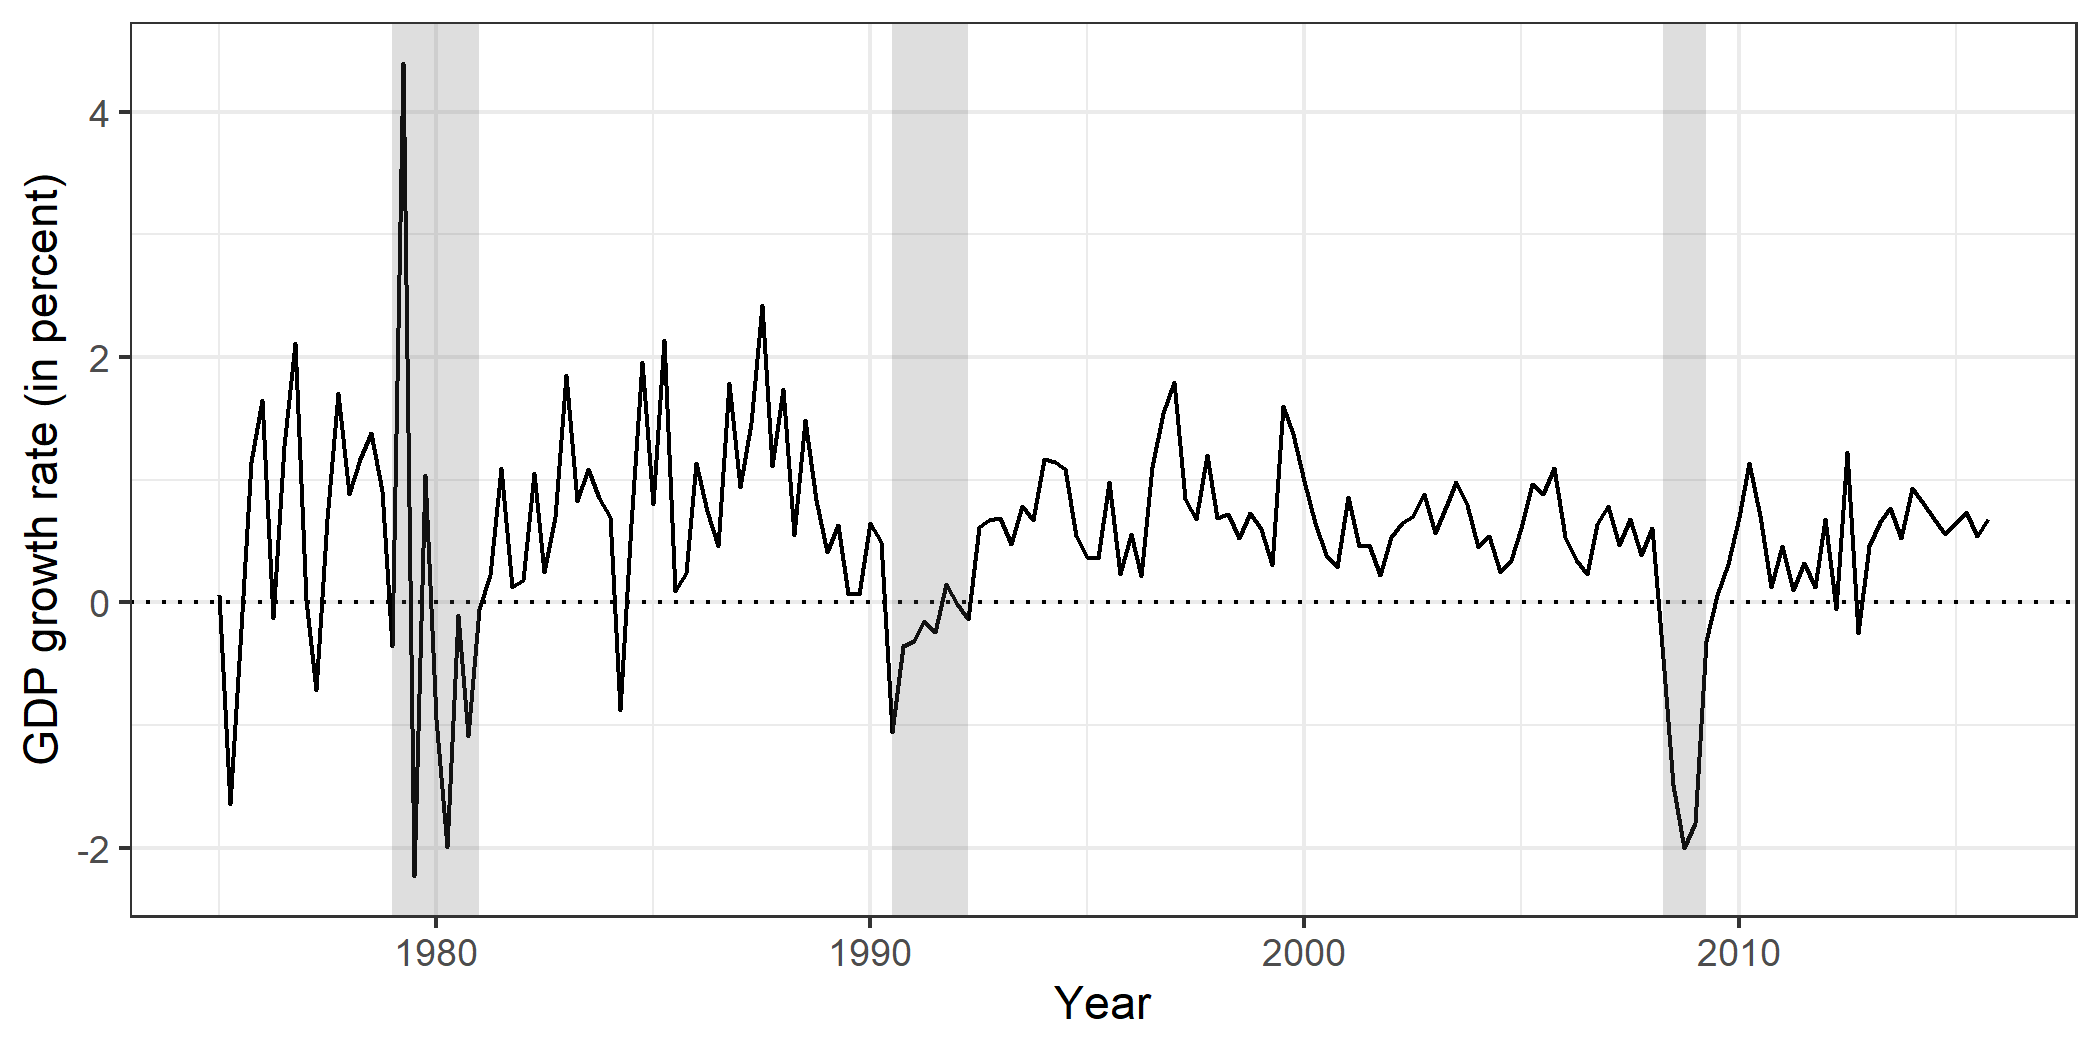
\includegraphics[width=\linewidth]{chap2/graphic/gdp-growth.png}
    \vspace{-3em}
	\justify\singlespacing\footnotesize{\textit{Notes:} This figure presents the quarterly GDP growth rate in the UK from 1975 to 2015. GDP is measured in chained volume and seasonally adjusted. Data are from the Office for National Statistics \href{https://www.ons.gov.uk/economy/grossdomesticproductgdp/timeseries/abmi/pn2}{Office for National Statistics}. Highlighted periods refer to recession periods in the UK.}
\end{figure}

Figure \ref{chap2-fig:lfs-national-cycle} presents the occupational dynamics for individuals born in the same years as our two cohorts using data from the LFS. Our estimates of probabilities for first-period and second-period occupations are performed at the start and the end of those curves. For the NCDS58, we consider their first period at age 23, hence in year 1981, which lies in a the Early 1980s recession. For other periods, they do not seem to be affected by business cycle dynamics as they follow the expected steady trends.
\begin{figure}[!htb]
    \centering
    \caption{LFS occupational dynamics over both cohort lifecycle}
    \label{chap2-fig:lfs-national-cycle}
    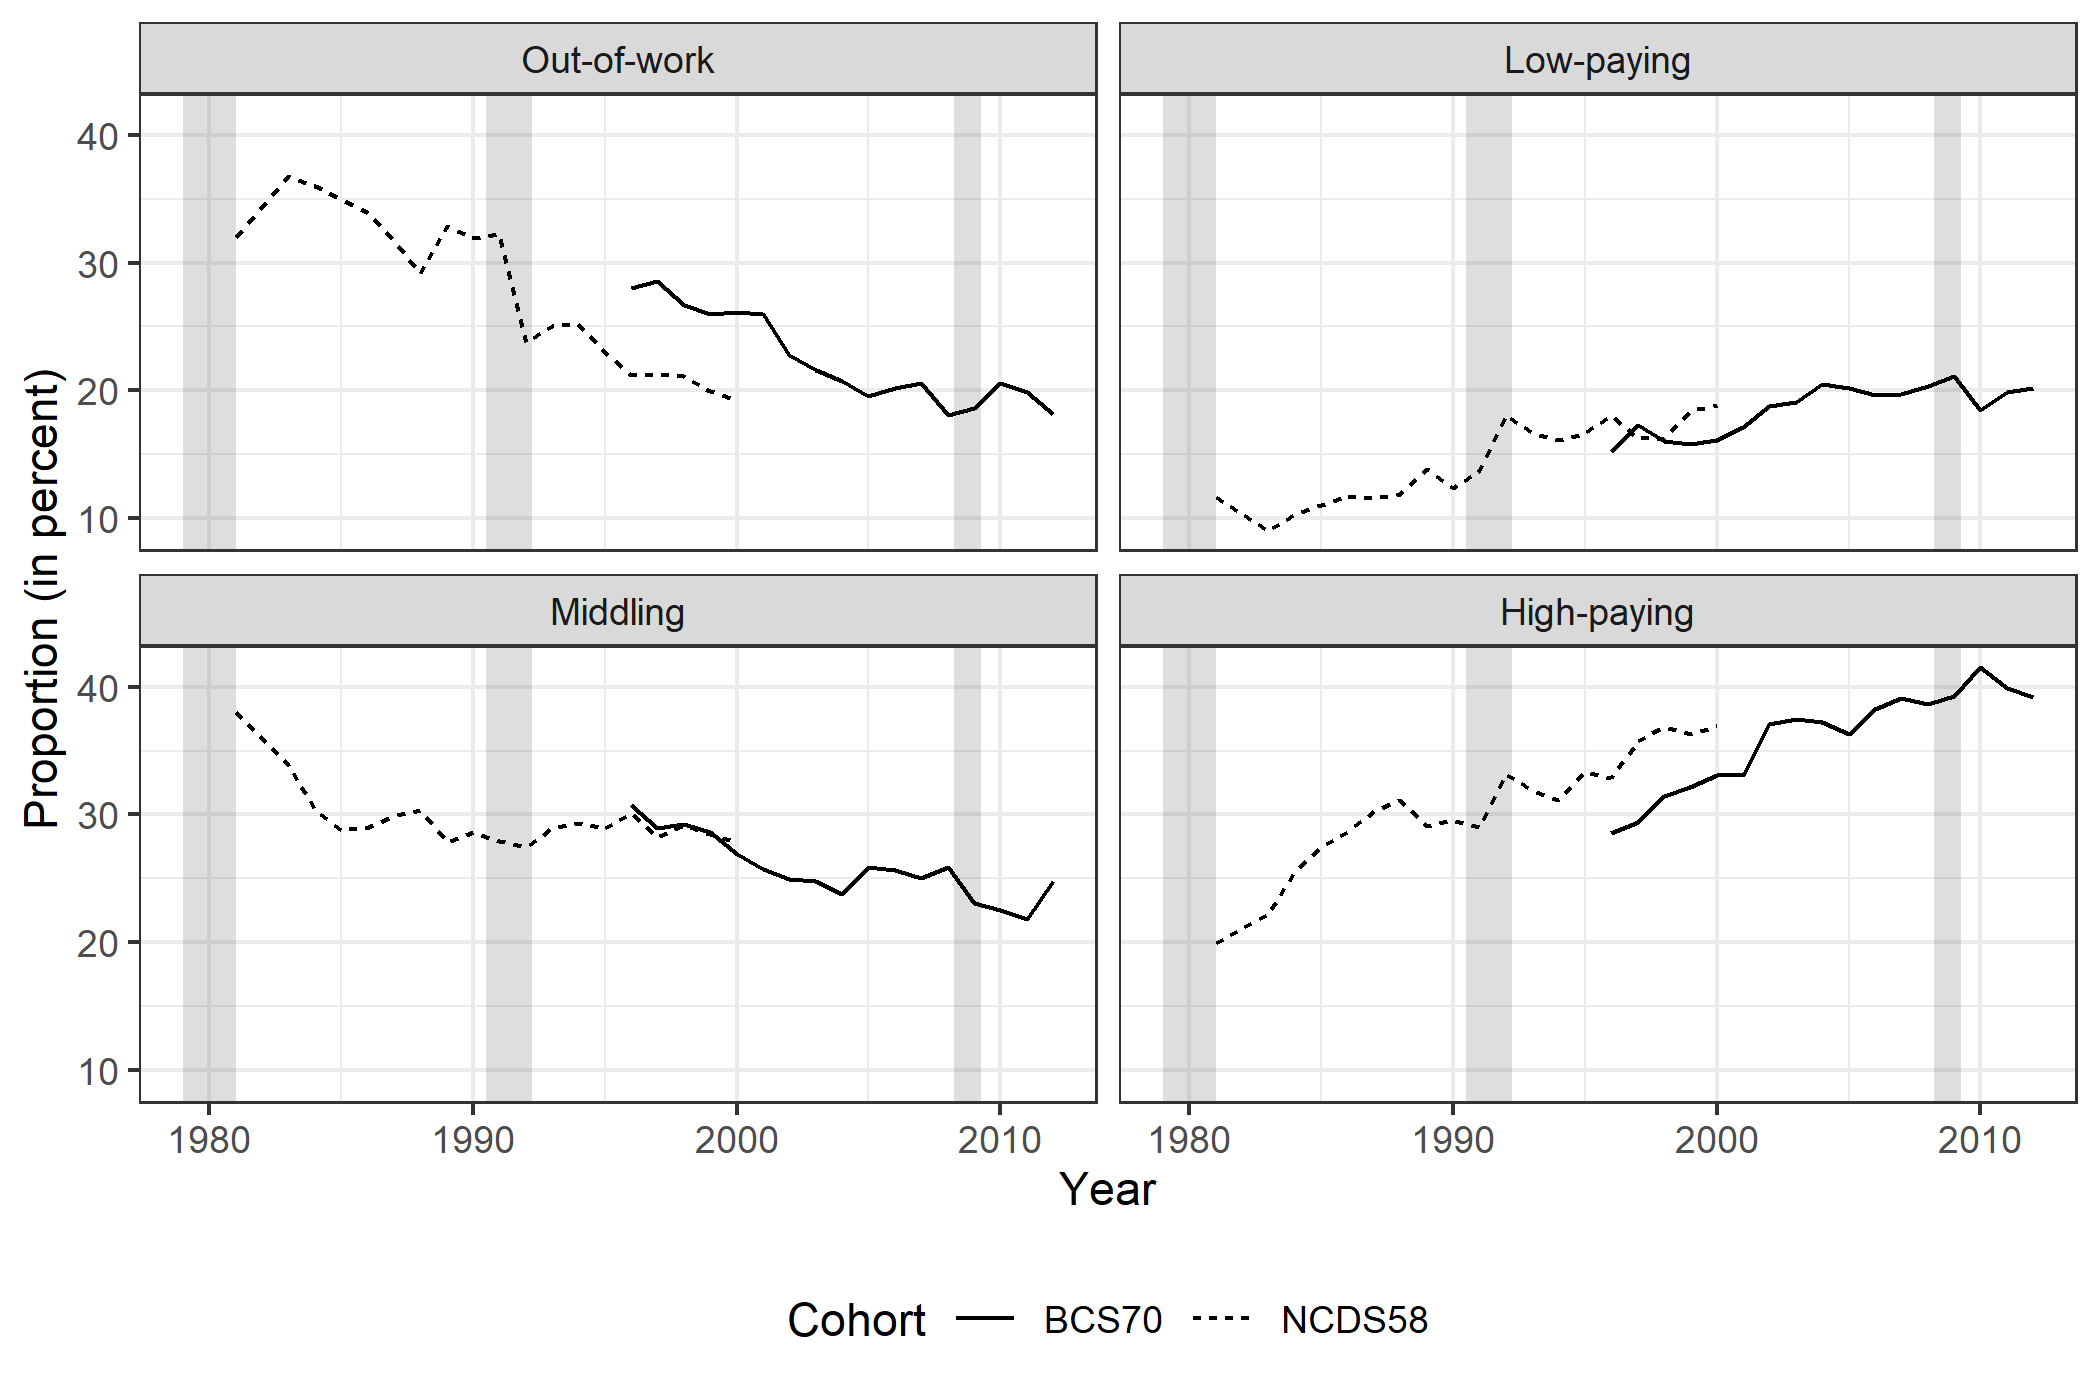
\includegraphics[width=\linewidth]{chap2/graphic/lfs-national-cycle.png}
    \vspace{-3em}
	\justify\singlespacing\footnotesize{\textit{Notes:} This figure presents the job polarization at the national level using the Labour Force Survey (LFS) data from 1981 to 2012. Curves represent the share of individuals in out-of-work, low-paying, middling, and high-paying occupations from the LFS for individuals born in the same year as the BCS70 and NCDS58 cohorts. Highlighted periods refer to recession periods in the UK.}
\end{figure}
The concern about the age of 23 as first period for the NCDS58 cohort can be addressed by looking at tables \ref{chap2-tab:rob2-multi1-base} and \ref{chap2-tab:rob2-multi3-base}. In those tables, we provide estimates of our main regressions when both cohorts are either 23 or 26 years old and show that our results are not driven by first-period age difference. The older cohort is age 26 in 1984 which does not lie in the Early 1980s recession.

\end{refsection}